% Options for packages loaded elsewhere
\PassOptionsToPackage{unicode}{hyperref}
\PassOptionsToPackage{hyphens}{url}
\PassOptionsToPackage{dvipsnames,svgnames,x11names}{xcolor}
%
\documentclass[
]{article}
\usepackage{amsmath,amssymb}
\usepackage{iftex}
\ifPDFTeX
  \usepackage[T1]{fontenc}
  \usepackage[utf8]{inputenc}
  \usepackage{textcomp} % provide euro and other symbols
\else % if luatex or xetex
  \usepackage{unicode-math} % this also loads fontspec
  \defaultfontfeatures{Scale=MatchLowercase}
  \defaultfontfeatures[\rmfamily]{Ligatures=TeX,Scale=1}
\fi
\usepackage{lmodern}
\ifPDFTeX\else
  % xetex/luatex font selection
\fi
% Use upquote if available, for straight quotes in verbatim environments
\IfFileExists{upquote.sty}{\usepackage{upquote}}{}
\IfFileExists{microtype.sty}{% use microtype if available
  \usepackage[]{microtype}
  \UseMicrotypeSet[protrusion]{basicmath} % disable protrusion for tt fonts
}{}
\makeatletter
\@ifundefined{KOMAClassName}{% if non-KOMA class
  \IfFileExists{parskip.sty}{%
    \usepackage{parskip}
  }{% else
    \setlength{\parindent}{0pt}
    \setlength{\parskip}{6pt plus 2pt minus 1pt}}
}{% if KOMA class
  \KOMAoptions{parskip=half}}
\makeatother
\usepackage{xcolor}
\usepackage[margin=1in]{geometry}
\usepackage{longtable,booktabs,array}
\usepackage{calc} % for calculating minipage widths
% Correct order of tables after \paragraph or \subparagraph
\usepackage{etoolbox}
\makeatletter
\patchcmd\longtable{\par}{\if@noskipsec\mbox{}\fi\par}{}{}
\makeatother
% Allow footnotes in longtable head/foot
\IfFileExists{footnotehyper.sty}{\usepackage{footnotehyper}}{\usepackage{footnote}}
\makesavenoteenv{longtable}
\usepackage{graphicx}
\makeatletter
\def\maxwidth{\ifdim\Gin@nat@width>\linewidth\linewidth\else\Gin@nat@width\fi}
\def\maxheight{\ifdim\Gin@nat@height>\textheight\textheight\else\Gin@nat@height\fi}
\makeatother
% Scale images if necessary, so that they will not overflow the page
% margins by default, and it is still possible to overwrite the defaults
% using explicit options in \includegraphics[width, height, ...]{}
\setkeys{Gin}{width=\maxwidth,height=\maxheight,keepaspectratio}
% Set default figure placement to htbp
\makeatletter
\def\fps@figure{htbp}
\makeatother
\setlength{\emergencystretch}{3em} % prevent overfull lines
\providecommand{\tightlist}{%
  \setlength{\itemsep}{0pt}\setlength{\parskip}{0pt}}
\setcounter{secnumdepth}{5}
\newlength{\cslhangindent}
\setlength{\cslhangindent}{1.5em}
\newlength{\csllabelwidth}
\setlength{\csllabelwidth}{3em}
\newlength{\cslentryspacingunit} % times entry-spacing
\setlength{\cslentryspacingunit}{\parskip}
\newenvironment{CSLReferences}[2] % #1 hanging-ident, #2 entry spacing
 {% don't indent paragraphs
  \setlength{\parindent}{0pt}
  % turn on hanging indent if param 1 is 1
  \ifodd #1
  \let\oldpar\par
  \def\par{\hangindent=\cslhangindent\oldpar}
  \fi
  % set entry spacing
  \setlength{\parskip}{#2\cslentryspacingunit}
 }%
 {}
\usepackage{calc}
\newcommand{\CSLBlock}[1]{#1\hfill\break}
\newcommand{\CSLLeftMargin}[1]{\parbox[t]{\csllabelwidth}{#1}}
\newcommand{\CSLRightInline}[1]{\parbox[t]{\linewidth - \csllabelwidth}{#1}\break}
\newcommand{\CSLIndent}[1]{\hspace{\cslhangindent}#1}
\usepackage{ragged2e}
\usepackage{setspace}
\usepackage{tocloft}
\usepackage{float}
\floatplacement{figure}{H}
\usepackage{wrapfig}
\usepackage{pdfpages}
\usepackage{caption}
\usepackage{booktabs}
\usepackage{longtable}
\usepackage{array}
\usepackage{multirow}
\usepackage{wrapfig}
\usepackage{float}
\usepackage{colortbl}
\usepackage{pdflscape}
\usepackage{tabu}
\usepackage{threeparttable}
\usepackage{threeparttablex}
\usepackage[normalem]{ulem}
\usepackage{makecell}
\usepackage{xcolor}
\ifLuaTeX
  \usepackage{selnolig}  % disable illegal ligatures
\fi
\IfFileExists{bookmark.sty}{\usepackage{bookmark}}{\usepackage{hyperref}}
\IfFileExists{xurl.sty}{\usepackage{xurl}}{} % add URL line breaks if available
\urlstyle{same}
\hypersetup{
  colorlinks=true,
  linkcolor={black},
  filecolor={Maroon},
  citecolor={Blue},
  urlcolor={Blue},
  pdfcreator={LaTeX via pandoc}}

\author{}
\date{\vspace{-2.5em}}

\begin{document}

\thispagestyle{empty}
\begin{singlespace} 
\begin{center}

\Huge

\textbf{HERE GOES YOUR TITLE}

\Large

\vspace{8mm}

by

\vspace{8mm}

\huge

Here Goes Your Name

\Large

\vspace{8mm}

Undergraduate degree

Master degree

\vspace{10mm}

A DISSERTATION SUBMITTED IN PARTIAL FULFILLMENT OF THE REQUIREMENTS FOR THE DEGREE OF

\vspace{5mm}

HERE GOES YOUR DEGREEE

\vspace{5mm}
in

\vspace{5mm}

THE FACULTY OF GRADUATE AND POSTDOCTORAL STUDIES

\vspace{5mm}

(Program)

\vspace{5mm}

THE UNIVERSITY OF BRITISH COLUMBIA

\vspace{5mm}

(Vancouver)

\vspace{6mm}

Month YYYY

© Here Goes Your Name, YYYY

\end{center}
\end{singlespace}
\normalsize
\clearpage

\pagenumbering{roman}
\setcounter{page}{2}

\doublespacing

The following individuals certify that they have read, and recommend to the Faculty of Graduate
and Postdoctoral Studies for acceptance, the dissertation entitled:

\vspace{5mm}

\noindent\underline{\makebox[6in][l]{Insert your dissertation title here}}\\
\vspace{2mm}

submitted by \underline{Insert Your Name Here} in partial fulfillment of the requirements for

the degree of \noindent\underline{\makebox[5in][l]{Name of your Degree}}

in \noindent\underline{\makebox[5.8in][l]{Insert Program}}

\vspace{5mm}

\textbf{Examining Committee:}

\noindent\underline{\makebox[6in][l]{Name of your Supervisor}}\\
Supervisor

\noindent\underline{\makebox[6in][l]{Name of your Committee Member}}\\
Supervisory Committee Member

\noindent\underline{\makebox[6in][l]{Name of University Examiner}}\\
University Examiner

\noindent\underline{\makebox[6in][l]{Name of University Examiner}}\\
University Examiner

\noindent\underline{\makebox[6in][l]{Name of External Examiner}}\\
External Examiner

\textbf{Additional Supervisory Committee Members:}

\noindent\underline{\makebox[6in][l]{Name of your Committee Member}}\\
Supervisory Committee Member

\clearpage

\setlength{\parindent}{4em} 
\linespread{1}
\doublespacing

\section*{Abstract}
\addcontentsline{toc}{section}{Abstract}

Lorem ipsum dolor sit amet, consectetur adipiscing elit. Nulla eleifend odio odio, et consectetur nunc commodo vitae. Donec eu finibus lacus. Integer at porta nulla. Fusce dignissim gravida lacinia. Nulla ut odio in ante imperdiet placerat. Maecenas vel imperdiet lorem. Proin ultricies, ex at bibendum fringilla, neque libero malesuada sem, in tincidunt leo mi vel mi. Phasellus scelerisque sagittis urna sed sodales. Curabitur iaculis justo velit, ultricies euismod justo convallis non. Nunc id purus et ante iaculis dignissim vel non erat. Donec dignissim urna ut lobortis congue. Nulla tempus ut ipsum non ornare. Donec ac purus nec sem cursus eleifend. Suspendisse potenti. Vestibulum ac vehicula ante.

Donec pulvinar a est ut vulputate. In id euismod nisi. Curabitur pulvinar bibendum convallis. Phasellus luctus posuere quam, a dapibus massa tristique in. Sed fermentum fermentum velit non sodales. Donec eget efficitur turpis. Sed ligula diam, ultrices porta vestibulum sed, varius maximus erat. Sed sagittis ut nisi ac tincidunt. Aliquam augue elit, egestas eu commodo ut, eleifend et nulla. Phasellus mollis lacus ac tortor fringilla, eget viverra enim sagittis. Morbi facilisis porttitor dui, eget elementum tellus malesuada ac. Integer sed accumsan lorem. Cras placerat ultrices libero at efficitur. Orci varius natoque penatibus et magnis dis parturient montes, nascetur ridiculus mus.

Nullam magna elit, sodales eu massa a, rutrum gravida orci. Mauris cursus odio turpis, et dignissim neque rutrum sit amet. Mauris vel nibh enim. Vestibulum tempus et lectus quis tempor. Proin dictum dui luctus felis sodales porttitor. Maecenas viverra vestibulum tristique. Nulla facilisi. Quisque efficitur lacus diam. Phasellus eget ligula quis mauris fermentum feugiat. Duis vitae lectus porttitor, vestibulum velit a, tincidunt nulla. Donec pharetra erat et urna sollicitudin, ac iaculis quam pulvinar. Donec pulvinar justo maximus lacinia sodales. Etiam sit amet diam vel ligula tempor congue nec in libero. Donec arcu risus, posuere.

\clearpage

\section*{Lay Summary}
\addcontentsline{toc}{section}{Lay Summary}

Lorem ipsum dolor sit amet, consectetur adipiscing elit. Sed lorem massa, suscipit vel dapibus a, iaculis ut sapien. Duis eu tellus vitae ligula semper commodo. Morbi felis tortor, ullamcorper vitae venenatis sit amet, commodo eu tortor. Proin ultrices ipsum ipsum, sed viverra arcu maximus eget. Aliquam nec nisl rutrum quam tempus iaculis nec sed dui. Nulla vitae imperdiet neque. Morbi eget eleifend lectus. Etiam semper id purus et scelerisque. Suspendisse lectus libero, iaculis et arcu vel, mattis mollis odio.

Phasellus quis metus erat. Nunc erat mi, posuere eleifend tortor quis, consequat dignissim metus. Pellentesque eget ante massa. Integer ultrices pulvinar varius. Sed dapibus sed arcu sit amet cursus. In hac habitasse platea dictumst. Aliquam vehicula est sed velit dapibus commodo. Donec placerat eu metus vel efficitur. Pellentesque commodo, nisi at elementum sagittis, erat magna feugiat elit, sit amet facilisis est diam eget tellus. Ut tellus velit, fringilla non consequat ut.

\clearpage

\section*{Preface}
\addcontentsline{toc}{section}{Preface}

Lorem ipsum dolor sit amet, consectetur adipiscing elit. Cras id nulla malesuada, auctor arcu at, tempor nibh. Etiam ultricies dictum nisi eu vulputate. Suspendisse tempor aliquam efficitur. Curabitur eget orci ac purus hendrerit laoreet. Proin porta arcu nisl, a fermentum tellus suscipit et. Nulla mattis orci ac tortor facilisis venenatis. Phasellus a velit tristique, tincidunt purus id, aliquet tellus. Orci varius natoque penatibus et magnis dis parturient montes, nascetur ridiculus mus. Sed et turpis sed odio faucibus aliquam nec eget est.

Phasellus ligula lacus, euismod posuere pretium sit amet, ornare condimentum nisl. Integer eu aliquet lectus, sit amet sagittis turpis. Etiam tempus bibendum nibh, eu accumsan sapien. Suspendisse tincidunt sit amet nisi vel consectetur. Donec vitae odio elit. Quisque dignissim risus feugiat nunc tempor hendrerit. Fusce consequat lectus eget felis tempus, et lobortis ante ornare. Etiam euismod quam eu scelerisque mattis. Praesent nisi lectus, tincidunt nec sapien ac, fermentum pellentesque orci.

Praesent semper faucibus mauris, in suscipit quam mattis et. Curabitur malesuada placerat magna. Morbi eget bibendum purus, sollicitudin faucibus enim. Donec condimentum arcu quis eros placerat sodales. Nunc non elit sodales, blandit risus vel, mattis odio. Nullam in aliquet ligula, ut viverra enim. Aliquam viverra justo non neque consequat dictum. Nunc tempor arcu sem, non blandit nisl dapibus eu. Donec vitae pretium magna. Nam risus augue, ultricies ac sollicitudin ut, rutrum eleifend purus. Donec lorem turpis, lacinia quis pretium non, sollicitudin eu enim. Curabitur eu eros congue, vehicula ante vitae, semper elit.

Fusce feugiat consectetur erat, nec venenatis massa malesuada nec. Curabitur varius convallis sem eget efficitur. Morbi congue odio non turpis cursus efficitur. In hac habitasse platea dictumst. Cras porttitor porttitor nibh id tempor. Sed bibendum quam nisl, sed congue lectus condimentum et. Curabitur nec mauris sapien. Morbi dictum ex sodales turpis ornare mattis. Suspendisse potenti. Pellentesque commodo lorem purus, id mattis nibh efficitur et. Cras tempus rutrum interdum. Vestibulum ante ipsum primis in faucibus orci luctus et ultrices posuere cubilia curae; Mauris placerat ligula eu nisl sagittis consequat. Curabitur placerat, elit quis cursus tempor, mauris augue posuere metus, ut elementum orci diam maximus lectus. Proin sed sodales nulla. Maecenas non sapien nec mauris facilisis fringilla.

\clearpage

\phantomsection 

\addcontentsline{toc}{section}{Table of Contents}
\renewcommand*\contentsname{Table of Contents}

\thispagestyle{empty}
\begin{singlespace}
\renewcommand{\cftsecleader}{\cftdotfill{\cftdotsep}}
\setcounter{tocdepth}{3}
\tableofcontents
\clearpage
\phantomsection
\addcontentsline{toc}{section}{List of Tables}
\listoftables
\clearpage
\phantomsection
\addcontentsline{toc}{section}{List of Figures}
\listoffigures
\clearpage
\end{singlespace}

\section*{Glossary}
\addcontentsline{toc}{section}{Glossary}

\begin{longtable}{>{}ll}

\textbf{AT1} & type I alveolar epithelial cell\\
\textbf{AT2} & type II alveolar epithelial cell\\
\textbf{AUC} & area under receiver operating curve\\
\textbf{BER} & balanced error rate\\
\textbf{COP} & cryptogenic organizing pneumonia\\
\addlinespace
\textbf{COPD} & chronic obstructive pulmonary disease\\
\textbf{CPFE} & combined pulmonary fibrosis and emphysema\\
\textbf{CTD-ILD} & connective tissue disease-associated interstitial lung disease\\
\textbf{DEG} & differentially expressed gene\\
\textbf{DESMOND} & Differentially ExpresSsed gene Modules iN Diseases\\
\addlinespace
\textbf{DIP} & desquamative interstitial pneumonia\\
\textbf{DLCO} & diffusing capacity for carbon monoxide\\
\textbf{ECM} & extracellular matrix\\
\textbf{EMT} & epithelial-mesenchymal transition\\
\textbf{FVC} & forced vital capacity\\
\addlinespace
\textbf{GEO} & Gene Expression Omnibus\\
\textbf{GO} & Gene Ontology\\
\textbf{HP} & hypersensitivity pneumonitis\\
\textbf{HRCT} & high-resolution computed tomography\\
\textbf{ILD} & interstitial lung disease\\
\addlinespace
\textbf{IPAF} & interstitial pneumonia with autoimmune features\\
\textbf{IPD} & individual participant data\\
\textbf{IPF} & idiopathic pulmonary fibrosis\\
\textbf{LTRC} & Lung Tissue Research Consortium\\
\textbf{MDD} & multidisciplinary discussion\\
\addlinespace
\textbf{MINT} & Multivariate INTegrative\\
\textbf{NSIP} & non-specific interstitial pneumonia\\
\textbf{PBMC} & peripheral blood mononuclear cells\\
\textbf{PPF} & progressive pulmonary fibrosis\\
\textbf{PRISMA} & Preferred Reporting Items for Systematic Reviews and Meta-Analyses\\
\addlinespace
\textbf{RA-ILD} & rheumatoid arthritis-associated interstitial lung disease\\
\textbf{RB-ILD} & respiratory bronchiolitis-interstitial lung disease\\
\textbf{RNA-seq} & RNA sequencing\\
\textbf{RRA} & robust rank aggregation\\
\textbf{SRA} & Sequence Read Archive\\
\addlinespace
\textbf{SSc-ILD} & systemic sclerosis-associated interstitial lung disease\\
\textbf{TMM} & trimmed mean of M values\\
\textbf{UIP} & usual interstitial pneumonia\\
\textbf{UnPaSt} & unsupervised patient stratification\\
\textbf{scRNA-seq} & single cell RNA-sequencing\\

\end{longtable}

\clearpage

\section*{Acknowledgements}
\addcontentsline{toc}{section}{Acknowledgements}

Lorem ipsum dolor sit amet, consectetur adipiscing elit. Cras id nulla malesuada, auctor arcu at, tempor nibh. Etiam ultricies dictum nisi eu vulputate. Suspendisse tempor aliquam efficitur. Curabitur eget orci ac purus hendrerit laoreet. Proin porta arcu nisl, a fermentum tellus suscipit et. Nulla mattis orci ac tortor facilisis venenatis. Phasellus a velit tristique, tincidunt purus id, aliquet tellus. Orci varius natoque penatibus et magnis dis parturient montes, nascetur ridiculus mus. Sed et turpis sed odio faucibus aliquam nec eget est.

Phasellus ligula lacus, euismod posuere pretium sit amet, ornare condimentum nisl. Integer eu aliquet lectus, sit amet sagittis turpis. Etiam tempus bibendum nibh, eu accumsan sapien. Suspendisse tincidunt sit amet nisi vel consectetur. Donec vitae odio elit. Quisque dignissim risus feugiat nunc tempor hendrerit. Fusce consequat lectus eget felis tempus, et lobortis ante ornare. Etiam euismod quam eu scelerisque mattis. Praesent nisi lectus, tincidunt nec sapien ac, fermentum pellentesque orci.

Praesent semper faucibus mauris, in suscipit quam mattis et. Curabitur malesuada placerat magna. Morbi eget bibendum purus, sollicitudin faucibus enim. Donec condimentum arcu quis eros placerat sodales. Nunc non elit sodales, blandit risus vel, mattis odio. Nullam in aliquet ligula, ut viverra enim. Aliquam viverra justo non neque consequat dictum. Nunc tempor arcu sem, non blandit nisl dapibus eu. Donec vitae pretium magna. Nam risus augue, ultricies ac sollicitudin ut, rutrum eleifend purus. Donec lorem turpis, lacinia quis pretium non, sollicitudin eu enim. Curabitur eu eros congue, vehicula ante vitae, semper elit.

Fusce feugiat consectetur erat, nec venenatis massa malesuada nec. Curabitur varius convallis sem eget efficitur. Morbi congue odio non turpis cursus efficitur. In hac habitasse platea dictumst. Cras porttitor porttitor nibh id tempor. Sed bibendum quam nisl, sed congue lectus condimentum et. Curabitur nec mauris sapien. Morbi dictum ex sodales turpis ornare mattis. Suspendisse potenti. Pellentesque commodo lorem purus, id mattis nibh efficitur et. Cras tempus rutrum interdum. Vestibulum ante ipsum primis in faucibus orci luctus et ultrices posuere cubilia curae; Mauris placerat ligula eu nisl sagittis consequat. Curabitur placerat, elit quis cursus tempor, mauris augue posuere metus, ut elementum orci diam maximus lectus. Proin sed sodales nulla. Maecenas non sapien nec mauris facilisis fringilla.

\clearpage

\section*{Dedication}
\addcontentsline{toc}{section}{Dedication}

\begin{center}
    \vspace*{\fill}
    Insert here your dedication
    \vspace*{\fill}
\end{center}

\clearpage

\hypertarget{introduction}{%
\section{Introduction}\label{introduction}}

\pagenumbering{arabic}

\renewcommand{\thefigure}{1.\arabic{figure}}
\setcounter{figure}{0}
\renewcommand{\thetable}{1.\arabic{table}}
\setcounter{table}{0}
\renewcommand{\theequation}{1.\arabic{equation}}
\setcounter{equation}{0}

In the 2018 diagnostic guidelines for idiopathic pulmonary fibrosis (IPF) released by a joint consortium of international respiratory societies (American Thoracic Society {[}ATS{]}, European Respiratory Society {[}ERS{]}, Japanese Respiraotry Society {[}JRS{]}, Asociación Latinoamericana del Tórax {[}ALAT{]}), a recommendation was made to investigate novel molecular biomarkers that could be integrated into clinical diagnosis {[}\protect\hyperlink{ref-raghu_diagnosis_2018}{1}{]}; in the 2022 update, a recommendation was not made for or against a genomic classifier identifying a usual interstitial pneumonia pattern diagnostic of IPF in transbronchial biopsies, thus highlighting the continued need for research into molecular biomarkers {[}\protect\hyperlink{ref-raghu_idiopathic_2022}{2}{]}. In this thesis, molecular biomarkers of interstitial lung diseases (ILDs) are investigated through a systematic review and meta-analysis of the literature, followed by gene expression profiling of blood samples taken from patients with ILD.

\hypertarget{interstitial-lung-disease}{%
\subsection{Interstitial Lung Disease}\label{interstitial-lung-disease}}

Fibrotic ILDs are debilitating restrictive lung diseases that result from excess deposition of extracellular matrix (ECM) within the lung interstitium, resulting in decreased oxygen uptake and subsequent functional limitation. Although ILDs can arise from a variety of causes (autoimmunity, environmental exposure), the most common subtype, IPF, is of unknown etiology. The incidence of IPF is 18.7 per 100,000 people in Canada, but increases to 39.5-156.4 per 100,000 people over the age of 60 -- a rate comparable to that of lung, breast, and prostate cancer (60.1, 129.9 and 120.8 per 100,000, respectively) {[}\protect\hyperlink{ref-canadian_cancer_statistics_advisory_committee_in_collaboration_with_the_canadian_cancer_society_statistics_canada_and_the_public_health_agency_of_canada_canadian_2023}{4}{]}. Patients with IPF have high morbidity, with quality of life scores in their first year of diagnosis comparable to those of patients with severe chronic obstructive pulmonary disease (COPD) {[}\protect\hyperlink{ref-hopkins_epidemiology_2016}{3}{]}. IPF patients are also at greater risk of comorbidities such as lung cancer, pulmonary hypertension, pulmonary embolisms {[}\protect\hyperlink{ref-raghu_comorbidities_2015}{5}{]}; acute exacerbations, which contribute significantly to the economic burden of the disease, can lead to respiratory failure and death {[}\protect\hyperlink{ref-hilberg_economic_2018}{7}{]}. Median survival for IPF is less than 5 years following diagnosis {[}\protect\hyperlink{ref-ley_clinical_2011}{8}{]}.

\hypertarget{mechanisms-of-ild}{%
\subsection{Mechanisms of ILD}\label{mechanisms-of-ild}}

A recurring hypothesis within the literature suggests that lung fibrosis is a result of repetitive injury to the alveoli, particularly type I alveolar epithelial cells (AT1s) which line the alveolar surface and are responsible for gas exchange. In the normal alveolus, type II alveolar epithelial cells (AT2s) secrete pulmonary surfactant to reduce surface tension within the alveoli, but AT2s undergo hyperplastic proliferation during stressful conditions such as injury. In addition to hyperplastic AT2s differentiating into AT1s via the TGF-β1 pathway, AT2s contribute to fibrosis via: 1) epithelial-mesenchymal transition (EMT) of AT2s to myofibroblasts; 2) apoptotic AT2s losing regulatory capacity over mesenchymal cells (fibroblasts), causing them to proliferate and produce more collagen; and 3) apoptotic AT2s releasing chemotactic factors such as CXCL12 to attract circulating fibrocytes, which invade the lung and expand the fibroblast pool {[}\protect\hyperlink{ref-bagnato_cellular_2015}{9}{]}.

Myofibroblasts and activated fibroblasts are the effector cells of fibrosis in ILD, producing and depositing ECM within the lung parenchyma in an uncontrolled manner. Both cell types are found in fibroblastic foci, which are key components of a usual interstitial pneumonia (UIP) histological pattern and are not found in healthy lung. Myofibroblasts, which differ from fibroblasts due to their expression of a-smooth muscle actin, may arise from the differentiation of resident fibroblasts, circulating fibrocytes, or mesenchymal transition from various other cell subsets {[}\protect\hyperlink{ref-marconi_epithelial-mesenchymal_2021}{10}{]}.

The most abundant immune cells in the lung (\textgreater70\%) are pulmonary macrophages. Alveolar macrophages (AM) reside within the alveoli and are the chief effector cells of immune responses, while interstitial macrophages (IM) reside within the lung parenchyma and maintain immune homeostasis {[}\protect\hyperlink{ref-byrne_pulmonary_2015}{11}{]}. In IPF, monocytes are `alternatively activated' towards the M2 phenotype through TH2-mediated immune responses, and produce profibrotic mediators such as TGF-b and PDGF {[}\protect\hyperlink{ref-zhu_m2_2017}{12}{]}.

\hypertarget{diagnosis-of-ild}{%
\subsection{Diagnosis of ILD}\label{diagnosis-of-ild}}

Current diagnostic guidelines for ILDs recommend a multidisciplinary discussion (MDD) between respirologists, radiologists, and pathologists. Patients with suspected ILDs frequently present with nonspecific symptoms, with a high-resolution computed tomography (HRCT) scan required to assess specific radiological patterns. A detailed history is taken with respect to exposure to mold, birds, and other exposures to identify potential causes of hypersensitivity pneumonitis (HP), and autoantibody panels are used to screen for autoimmune/connective tissue diseases. Identification of a UIP pattern on HRCT, which is characterized by bilateral reticulation and honeycombing in the periphery and lower lobes, is sufficient to confirm a diagnosis of IPF in patients with a compatible clinical presentation; however, there is substantial variability in HRCT interpretation among non-experts {[}\protect\hyperlink{ref-raghu_diagnosis_2018}{1}{]}.

A major diagnostic challenge within the ILD field is the identification of IPF. HRCT patterns are often nonspecific and fail to distinguish between IPF and non-IPF ILDs. Non-IPF ILDs, which include HP, connective tissue disease-related ILDs (systemic sclerosis-associated ILD (SSc- ILD), rheumatoid arthritis, Sjögren's syndrome, interstitial pneumonia with autoimmune features (IPAF)), drug-induced ILDs, and pneumoconiosis (occupational ILDs), are frequently treated with immunosuppressive medications {[}\protect\hyperlink{ref-lederer_idiopathic_2018}{13}{]}. In contrast, IPF patients require anti-fibrotic drug treatment (nintedanib, pirfenidone) and perform worse on immunosuppressives (e.g.~mycophenolate, azathioprine), thus highlighting the necessity to distinguish IPF from non-IPF ILDs. Specifically, IPF patients on glucocorticoid therapy showed no slowing of disease progression compared to placebo and, in contrast, had increased hospitalization and mortality {[}\protect\hyperlink{ref-idiopathic_pulmonary_fibrosis_clinical_research_network_prednisone_2012}{14}{]}. HRCT patterns indeterminate for radiological UIP can be followed up with a surgical lung biopsy (SLB) to identify a histopathological UIP pattern (honeycombing, fibroblastic foci, patchy fibrosis, paraseptal distribution) {[}\protect\hyperlink{ref-lynch_diagnostic_2018}{15}{]}. However, SLBs are associated with significant risks of mortality that increase with age, severely reduced lung function, and the presence of comorbidities. For these reasons, many patients with ILD are unable to undergo the most definitive diagnostic test.

The most challenging differential diagnosis involves distinguishing between IPF, HP, and IPAF. HP is the result of an immune response within the lung due to extended exposure to bacterial, fungal, animal, or insect proteins, which can eventually lead to fibrosis. A recent multi-centre study showed that inter-multidisciplinary teams disagreed the most when it came to diagnosing HP compared to other types of ILD, highlighting the difficulties associated with its nonspecific clinical presentation and resultant lack of established diagnostic criteria {[}\protect\hyperlink{ref-walsh_multicentre_2016}{16}{]}. IPAF is a newly proposed clinical designation that presents with features suggestive of an autoimmune condition, yet do not fulfill diagnostic criteria for any particular connective tissue disease {[}\protect\hyperlink{ref-graney_interstitial_2019}{17}{]}. When all diagnostic tools have been exhausted with no definitive diagnosis, patients are considered to have unclassifiable ILD, which occurs in approximately 15\% of ILD patients {[}\protect\hyperlink{ref-skolnik_unclassifiable_2016}{18}{]}. Treatment of unclassifiable ILD patients is particularly challenging with no clearly preferred option in the majority of these patients.

\hypertarget{progressive-pulmonary-fibrosis}{%
\subsection{Progressive pulmonary fibrosis}\label{progressive-pulmonary-fibrosis}}

Progressive pulmonary fibrosis (PPF) refers to a subset of non-IPF ILDs that display a similar disease progression to IPF, which is defined over time by a decline in lung function, worsening respiratory symptoms, and increased fibrosis as seen on HRCT. Numerous criteria have been proposed to define PPF:

\begin{enumerate}
\def\labelenumi{\arabic{enumi}.}
\tightlist
\item
  The 2022 ATS/ERS/JRS/ALAT IPF diagnostic guidelines {[}\protect\hyperlink{ref-raghu_idiopathic_2022}{2}{]} proposed a combination of two or more of the following over 1 year:
\end{enumerate}

\begin{itemize}
\tightlist
\item
  worsening respiratory symptoms;
\item
  physiological progression (defined by absolute decline in predicted forced vital capacity {[}FVC\%{]} \underline{>}5\% and/or predicted diffusing capacity for carbon monoxide {[}D\textsubscript{LCO}\%{]} \underline{>}10\%);
\item
  radiological progression (increased fibrosis on HRCT).
\end{itemize}

\begin{enumerate}
\def\labelenumi{\arabic{enumi}.}
\setcounter{enumi}{1}
\tightlist
\item
  The criteria for inclusion into the INBUILD trial {[}\protect\hyperlink{ref-flaherty_nintedanib_2019}{19}{]} was defined by meeting one of the following criteria for progressive disease within the past 24 months:
\end{enumerate}

\begin{itemize}
\tightlist
\item
  relative decline in FVC\% predicted of \underline{>}10\%;
\item
  relative decline in FVC\% predicted of 5-10\% and either worsening of respiratory symptoms or increased fibrosis on HRCT;
\item
  worsening of respiratory symptoms and radiological progression.
\end{itemize}

\begin{enumerate}
\def\labelenumi{\arabic{enumi}.}
\setcounter{enumi}{2}
\item
  The unclassifiable ILD (uILD) trial {[}\protect\hyperlink{ref-maher_pirfenidone_2020}{20}{]} included patients on the basis of an absolute decline in FVC\% of \underline{>}5\% or worsening respiratory symptoms within 6 months.
\item
  The RELIEF trial {[}\protect\hyperlink{ref-behr_pirfenidone_2021}{21}{]} included patients if they had an absolute annual decline in FVC\% of \underline{>}5\% with at least three measurements within 6-24 months.
\end{enumerate}

Retrospective analysis of various cohorts evaluating the above criteria have revealed that few patients meet all of the above definitions but each of them are associated with a poor prognosis {[}\protect\hyperlink{ref-khor_patient_2023}{22}{]}. Depending on the definition used for PPF, \textasciitilde18-32\% of non-IPF ILDs display this phenotype compared to \textasciitilde60\% of IPF patients {[}\protect\hyperlink{ref-rajan_progressive_2023}{27}{]}; nevertheless, identification is important as patients with PPF were shown to have a reduced annual rate of decline in FVC\% predicted after receiving nintedanib compared to placebo {[}\protect\hyperlink{ref-flaherty_nintedanib_2019}{19}{]}.

\hypertarget{objective}{%
\subsection{Objective}\label{objective}}

Better tools are needed for clinical management of ILDs. Currently, up to 55\% of ILD patients experience at least one misdiagnosis prior to MDD, and 43\% report a delay in diagnosis of at least one year {[}\protect\hyperlink{ref-grewal_role_2019}{29}{]}. These delays are problematic for clinical management, particularly with respect to administering correct pharmacotherapy, and it is unsurprising that delays in diagnosing IPF are associated with an increased risk of mortality {[}\protect\hyperlink{ref-lamas_delayed_2011}{30}{]}. Previous attempts to identify biomarkers of IPF have failed in part due to difficulties in reproducing reliable concentration cut-off thresholds to diagnose disease {[}\protect\hyperlink{ref-drakopanagiotakis_biomarkers_2018}{31}{]}. Promising IPF diagnostic biomarkers such as matrix metalloprotease-7 (MMP-7) are also elevated in the serum of patients with HP and other ILDs {[}\protect\hyperlink{ref-morais_serum_2015}{32}{]}, suggesting that candidate biomarkers are limited in their ability to discern disease subtype from the fibrotic process of ILD. Furthermore, patients with PPF have a poor prognosis and early adoption of anti-fibrotic therapy is shown to be beneficial, but criteria for identifying PPF has not yet been agreed upon and candidate guidelines are based on data obtained over the course of 1-2 years.

Given the inherent risks of lung biopsies in aging populations, the objective of this thesis is to investigate ILD blood for novel diagnostic and prognostic molecular biomarkers of ILD. This will be carried out by first performing a systematic review and meta-analysis of ILD transcriptomics (gene expression studies) to define currently understood molecular markers of ILD. Then, we will examine feasibility of using whole blood samples from ILD patients in a pilot study using a targeted gene assay, followed by a larger study examining whole blood ILD samples using bulk RNA-sequencing (RNA-seq). Finally, we will investigate single cell-level blood gene expression profiles.

\clearpage

\hypertarget{a-systematic-review-and-meta-analysis-of-ild-transcriptomics}{%
\section{A systematic review and meta-analysis of ILD transcriptomics}\label{a-systematic-review-and-meta-analysis-of-ild-transcriptomics}}

\renewcommand{\thefigure}{2.\arabic{figure}}
\setcounter{figure}{0}
\renewcommand{\thetable}{2.\arabic{table}}
\setcounter{table}{0}
\renewcommand{\theequation}{2.\arabic{equation}}
\setcounter{equation}{0}

High-performance gene expression analysis (transcriptomics) has been crucial in finding key biological processes involved in the pathogenesis of ILD, including matrix metalloproteinases, Wnt signaling, and cellular senescence {[}\protect\hyperlink{ref-vukmirovic_impact_2018}{33}{]}. Although molecules such as MMP-7 have been proposed as a diagnostic and prognostic biomarker of idiopathic pulmonary fibrosis (IPF) {[}\protect\hyperlink{ref-khan_systematic_2022}{34}{]}, molecular biomarkers are not yet widely used in clinical management of ILDs {[}\protect\hyperlink{ref-raghu_diagnosis_2018}{1},\protect\hyperlink{ref-morais_serum_2015}{32},\protect\hyperlink{ref-white_plasma_2016}{35}--\protect\hyperlink{ref-johannson_treatment_2021}{37}{]}. A genomic classifier based on transbronchial biopsies (Envisia) has been developed to identify the histological pattern of UIP, which allows for a diagnosis of IPF in matching clinical characteristics {[}\protect\hyperlink{ref-pankratz_usual_2017}{38},\protect\hyperlink{ref-choi_analytical_2017}{39}{]}. The clinical application of this genomic classifier is limited by its availability and its use has not been recommended in recent clinical practice guidelines {[}\protect\hyperlink{ref-raghu_idiopathic_2022}{2}{]}.

A majority of transcriptomics research has been performed in IPF, and many differentially expressed genes have been identified and reproduced across different studies. There are fewer investigations into other ILD subtypes, such as HP and connective tissue disease-associated ILD (CTD-ILD), and a consensus of molecular perturbations has yet to be determined for other ILDs. Furthermore, studies with adequate sample sizes are rare, also due to the cost of microarray and RNA-seq technologies. As sequencing throughput has improved and new approaches including single-cell RNA sequencing (scRNA-seq) are emerging, summarizing the findings of bulk tissue sequencing is likely valuable for comparison with future scRNA-seq findings. Hence, the objective of this systematic review and individual participant data (IPD) meta-analysis was to determine consensus gene expression signatures of patients with fibrotic ILD compared to control, and to identify and validate biomarkers for the classification of major fibrotic ILD subtypes.

\hypertarget{methods}{%
\subsection{Methods}\label{methods}}

\hypertarget{search-strategy}{%
\subsubsection{Search strategy}\label{search-strategy}}

In accordance with Preferred Reporting Items for Systematic Reviews and Meta-Analyses (PRISMA) guidelines, we performed a systematic review to identify transcriptomics studies focusing on fibrotic ILD samples and we registered the study with PROSPERO (CRD42018085682). Literature searches were performed in Medline and Embase on December 18th 2018, and updated on November 23rd 2023. Our search terms included variations of ``interstitial lung disease'', common ILD subtypes, as well as transcriptomics-related key words (\protect\hyperlink{search-terms}{Appendix A - Search terms}). Given the relative recency of transcriptomics technology, we limited our search to only include results published from the year 2000 and onwards. A similar strategy was adopted for searching the Gene Expression Omnibus (GEO). Screening of titles, abstracts, and full-text studies was performed by two independent reviewers (Daniel He and Sabina A Guler) using the online Covidence tool. We focused our search on common fibrotic ILDs in adults (IPF, HP, idiopathic nonspecific interstitial pneumonia (NSIP), and connective tissue disease-associated ILDs), as it was more likely that they would be investigated for gene expression. We included studies investigating transcriptomics of fibrotic ILDs via lung or blood sampling, and excluded those focused on isolated cell populations (i.e.~fibroblasts). To assess the risk of bias in the included studies, we used a modified checklist based on the criteria outlined by Dupuy and Simon {[}\protect\hyperlink{ref-dupuy_critical_2007}{40}{]} (see: \protect\hyperlink{qc}{Appendix A - Search terms}).

\hypertarget{data-extraction-integration-and-analysis}{%
\subsubsection{Data extraction, integration, and analysis}\label{data-extraction-integration-and-analysis}}

We extracted participant-level data from included studies using the data repository sites GEO, ArrayExpress and the Sequence Read Archive (SRA). Raw data were processed using recommended protocols from the `limma' package (v3.55.3) for microarrays (manufacturer-based) and RNA-seq (trimmed mean of M values, TMM) if author-provided normalized matrices were unavailable. Dataset quality was determined by examining distribution plots and comparing DEGs obtained from limma with reported values (data not shown), and outliers were removed if they were located more than 3 standard deviations away from the mean on the first and second principal components (Figure \ref{fig:outlierPCA}). In order to explore sex-specific ILD signatures, we examined expression of 1 female-specific gene (\textit{XIST}) located on the X chromosome and 4 male-specific genes (\textit{RPS4Y1}, \textit{EIF1AY}, \textit{DDX3Y}, \textit{KDM5D}) located on the Y chromosome to obtain the predicted sex for each sample. The sex provided in the metadata from the original publication did not match predicted sex in 31 of 1,441 samples (2.15\%); these samples were omitted from sex-specific analyses.

To synthesize transcriptomics data, we used an IPD approach to our meta-analysis using the Multivariate INTegrative (MINT) method (`mixOmics' v6.22.0), which is an integrative classification method based on partial least squares regression (PLS). A more detailed explanation of the methodology can be found in Rohart et al. {[}\protect\hyperlink{ref-rohart_mint_2017}{41},\protect\hyperlink{ref-rohart_mixomics_2017}{42}{]}. We benchmarked the MINT data integration by comparing it with differentially expressed gene (DEG) list integration through robust rank aggregation (RRA) {[}\protect\hyperlink{ref-kolde_robust_2012}{43}{]}, which also allowed for the inclusion of studies where raw data was unavailable (i.e.~older studies that may have used first-generation microarrays with limited gene coverage).

We used 24 of 32 datasets (from 31 studies) as a training set, and integrated them to develop classification models that were tuned via leave-one-group-out cross validation to have the lowest balanced error rate (BER; average error rate in each class) (Figure \ref{fig:tuningMINT}), and validated on the remaining eight held-out test datasets by examining area under receiver operating curve (AUC) and BER (Table \ref{tab:modelPerf}). Eight test sets were selected to cover 15-20\% of the total number of samples to create an 80/20 training/test split, in addition to balancing the number of microarray and RNA-seq studies, and to covering all ILD subtypes of interest (IPF, HP, NSIP, SSc-ILD), Lung Tissue Research Consortium (LTRC) and non-LTRC studies, American and non-American cohorts, and recently published datasets {[}\protect\hyperlink{ref-bauer_novel_2015}{44}--\protect\hyperlink{ref-jaffar_matrix_2022}{51}{]}. All data processing and analysis was performed in R (v4.2.3). Additional details on our methodology are provided in \protect\hyperlink{data}{Appendix A - Data integration and analysis}.

\hypertarget{biclustering}{%
\subsubsection{Biclustering}\label{biclustering}}

Transcriptomics datasets were concatenated and genes containing NA values were removed. ComBat (`sva' v3.46.0) was used to correct for study-specific batch effects, and biclusters of the batch-corrected matrix were identified using algorithms implemented in the `MoSBi' package (v1.4.0) {[}\protect\hyperlink{ref-rose_mosbi_2022}{52}{]}, as well as the unsupervised patient stratification (UnPaSt) algorithm, which is an unconstrained version of the Differentially ExpreSsed gene Modules iN Diseases (DESMOND) algorithm {[}\protect\hyperlink{ref-zolotareva_identification_2021}{53}{]}. Association between biclusters and clinical variables was assessed using a Chi-squared test (categorical; diagnostic class) or linear regression (continuous; predicted FVC\%, DLCO\%).

\hypertarget{results}{%
\subsection{Results}\label{results}}

\hypertarget{search-results}{%
\subsubsection{Search results}\label{search-results}}

From our initial search of medical literature databases (3,844 from MEDLINE and 6,624 from EMBASE) and a genomic database (215 from GEO), we assessed 196 records for eligibility and identified 43 studies that used transcriptomics to profile ILD samples (Figure \ref{fig:prisma}). Four studies investigated blood transcriptional profiles (IPF, HP, SSc-ILD) {[}\protect\hyperlink{ref-yang_peripheral_2012}{54}--\protect\hyperlink{ref-jia_interleukin_2023}{57}{]}, and four looked at gene expression profiles of peripheral blood mononuclear cells (PBMCs) from IPF and systemic sclerosis-associated ILD (SSc-ILD) {[}\protect\hyperlink{ref-huang_sphingosine-1-phosphate_2015}{58}--\protect\hyperlink{ref-assassi_peripheral_2022}{61}{]}. Of the remaining 35 studies that used transcriptomics to investigate fibrotic ILD lung samples, 24 studies reported DEGs between ILD and control, 29 studies uploaded publicly available data for analysis, and 20 studies had both (Table \ref{tab:datasets}). Eight datasets were associated with the LTRC, and duplicate LTRC samples across studies were removed where LTRC identifiers were available {[}\protect\hyperlink{ref-bauer_novel_2015}{44},\protect\hyperlink{ref-schafer_cellular_2017}{46},\protect\hyperlink{ref-cho_systems_2011}{62}--\protect\hyperlink{ref-borie_colocalization_2022}{69}{]}. The most commonly profiled fibrotic ILD subtype was IPF, appearing in all identified datasets except one, followed by idiopathic NSIP, fibrotic HP, and SSc-ILD. Classifiers for subtypes such as desquamative interstitial pneumonia (DIP), respiratory bronchiolitis-ILD (RB-ILD), and cryptogenic organizing pneumonia (COP) were not generated as these samples were few in number; classifiers for HP and SSc-ILD blood/PBMC samples were also not created due to insufficient numbers of datasets.

\captionsetup{width=6.5in}



\begin{figure}

{\centering 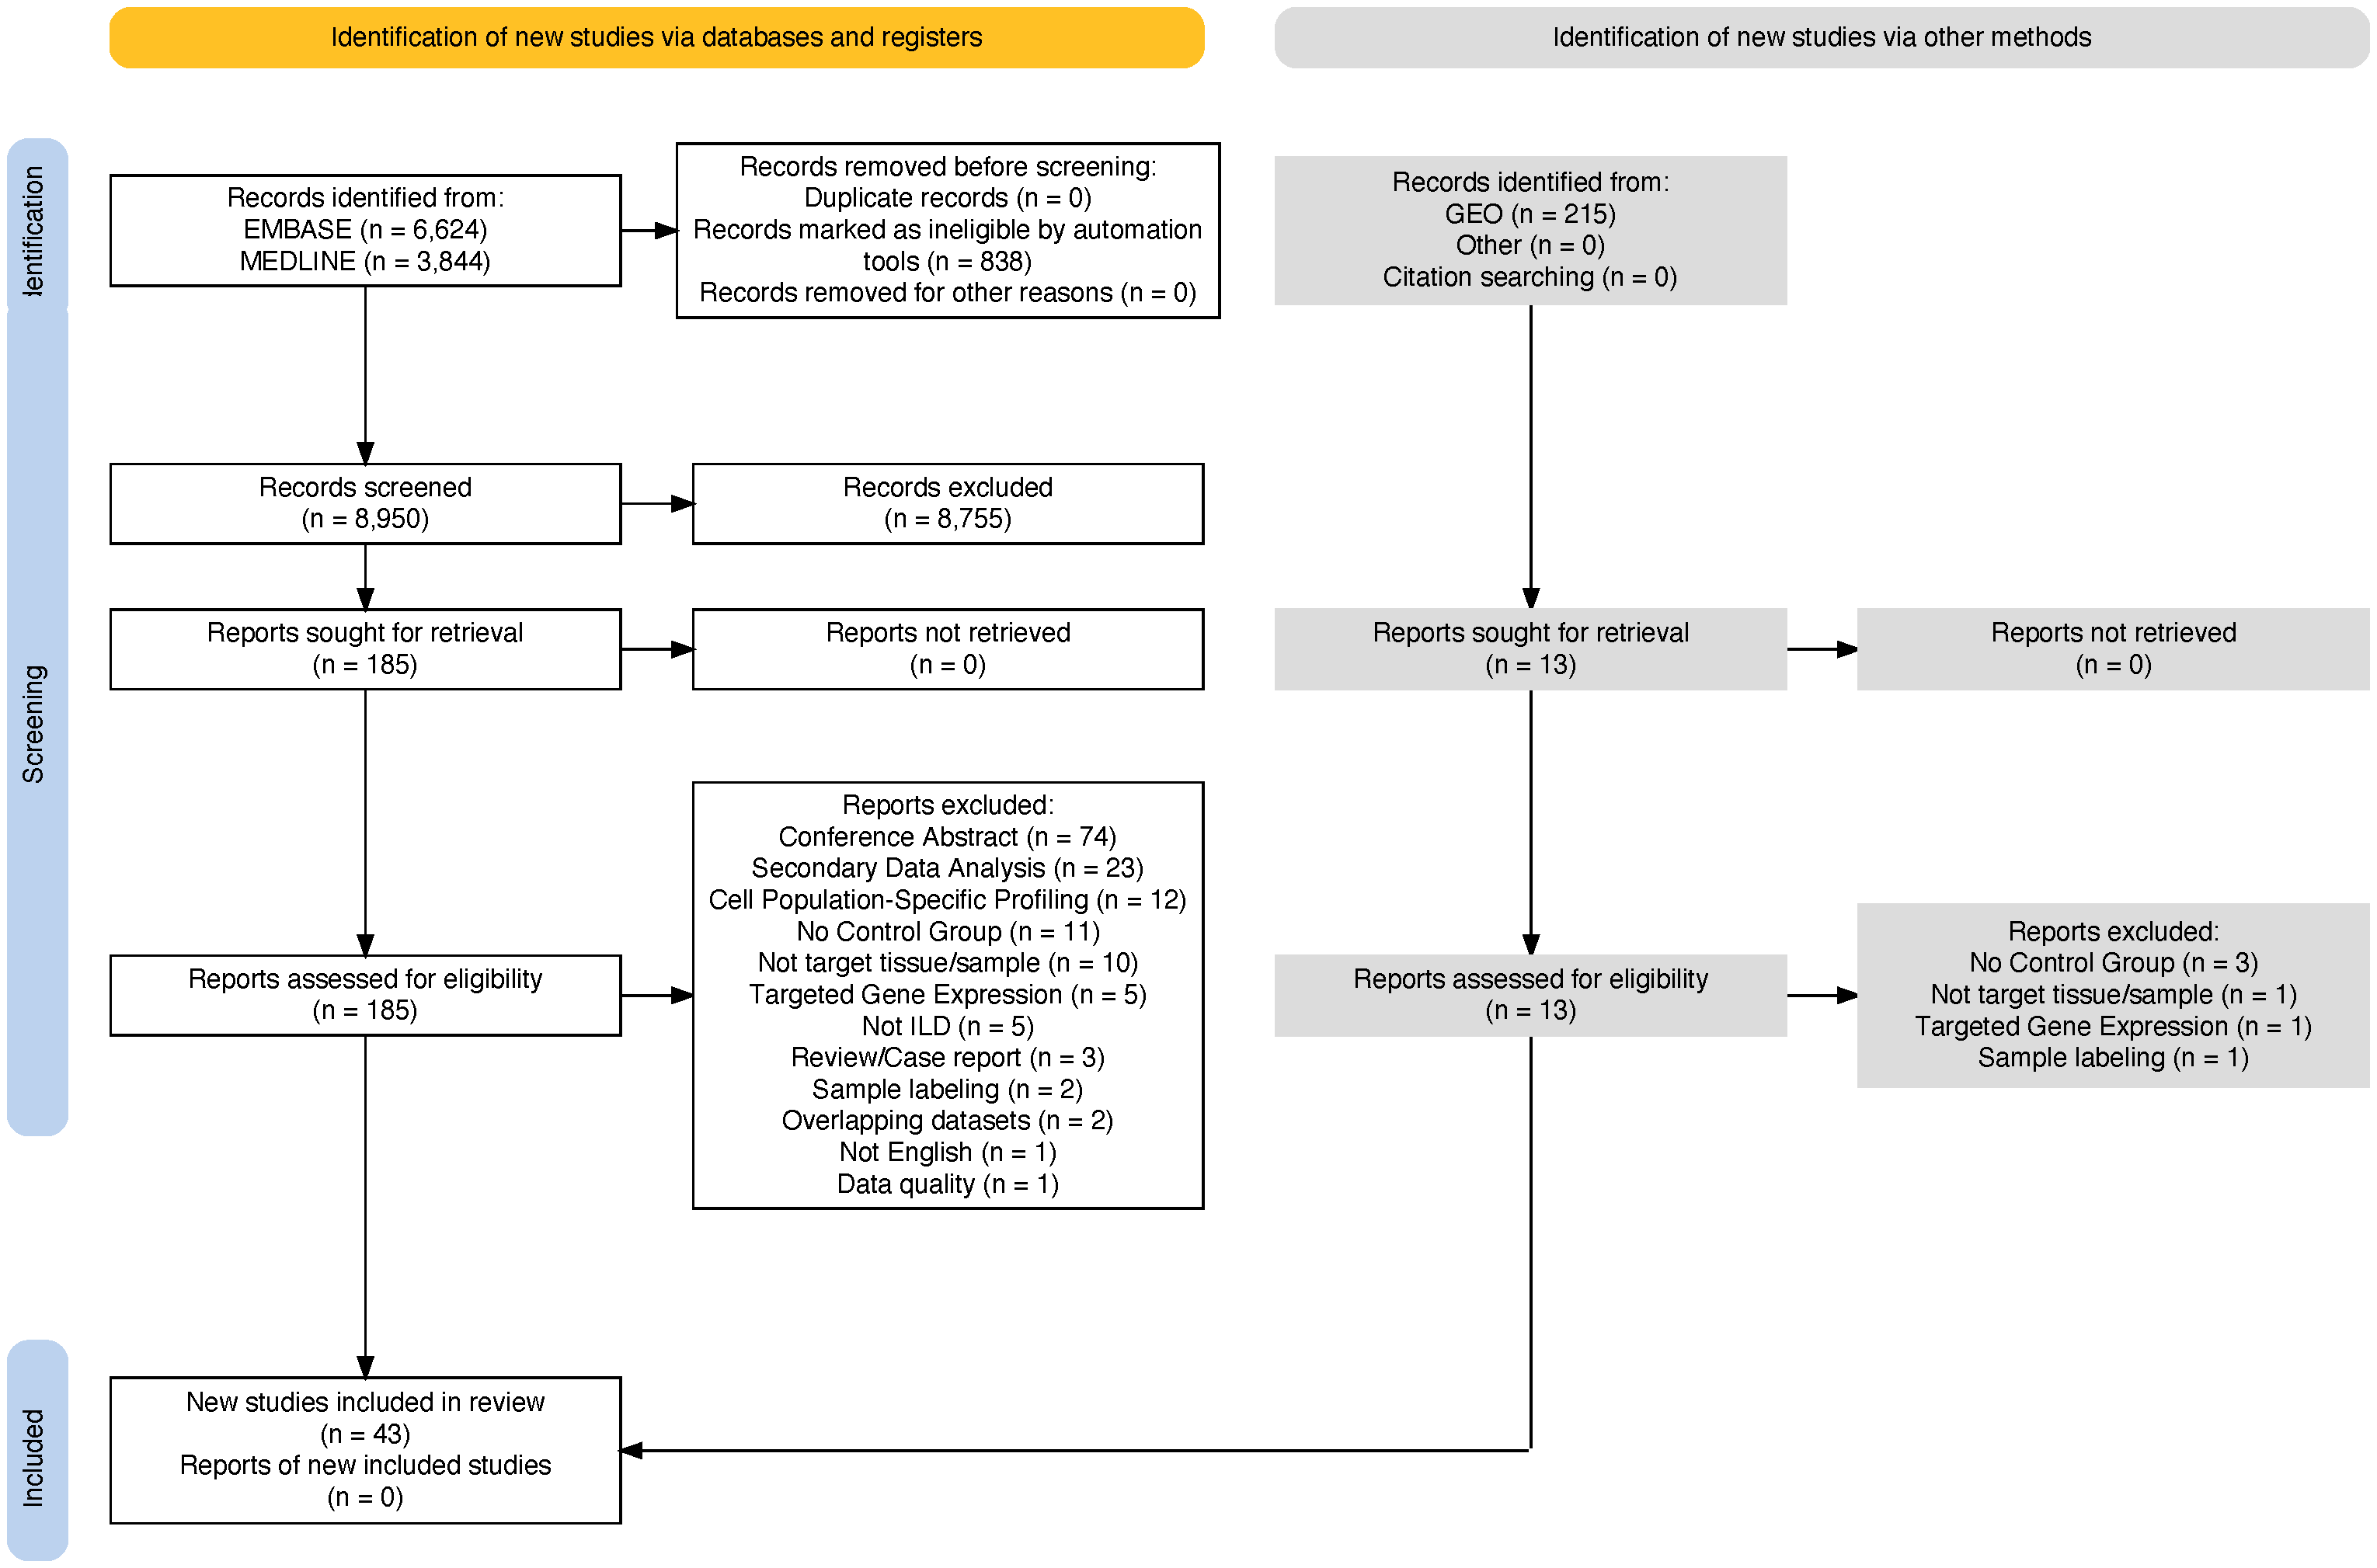
\includegraphics[width=0.9\linewidth,]{./Figures/SysReview/Figure1_Prisma} 

}

\caption[PRISMA screening]{\textbf{Preferred Reporting Items for Systematic Reviews and Meta-Analyses (PRISMA) flowchart of study identification and screening.} MEDLINE, EMBASE, and the Gene Expression Omnibus (GEO) were examined for studies using transcriptomics to investigate samples from patients with interstitial lung disease (ILD).}\label{fig:prisma}
\end{figure}

\hypertarget{lung-gene-expression-signatures-of-fibrotic-ild-subtypes}{%
\subsubsection{Lung gene expression signatures of fibrotic ILD subtypes}\label{lung-gene-expression-signatures-of-fibrotic-ild-subtypes}}

We created lung gene signatures for each fibrotic ILD subtype via classification models generated from our integrated datasets (Figure \ref{fig:integration}). In IPF, we identified a 55-gene signature using 23 training datasets (n=576 control, n=721 IPF), which was then validated on eight test datasets (n=107 control, n=193 IPF) with AUC=0.99 {[}0.99-1.00{]} (Figure \ref{fig:mintmodel}A, Table \ref{tab:ipfgenes}). To confirm the validity of MINT in identifying relevant DEGs, we compared our IPF vs Control signature against an IPF vs Control aggregate DEG list generated by RRA and found that 39 of the 55 genes were shared, including \textit{COMP}, \textit{DIO2}, \textit{MMP7} (IPF upregulated), \textit{CA4}, \textit{FAM167A}, and \textit{MYRF} (IPF downregulated) (Figure \ref{fig:modelUpset}A). For the peripheral transcriptome, we generated a classification model of IPF vs Control for whole blood datasets, which was validated on two PBMC datasets (AUC=0.74 {[}0.67-0.81{]}); likewise, a classification model of IPF vs Control for PBMCs was validated on two whole blood datasets (AUC=0.73 {[}0.65-0.81{]}) (Figure \ref{fig:bloodmodel}, Table \ref{tab:ipfgenesblood}, Table \ref{tab:ipfgenespbmc}). We also performed sex-specific analyses for IPF, HP, and NSIP by inferring sex from sex-specific genes, showing good performance for between-sex comparisons with the exception of the male NSIP classification model (male test set: AUC=0.98 {[}0.93-1.00{]}; female test set: AUC=0.79 {[}0.68-0.90) (Table \ref{tab:sexModel}).

\newpage





































\captionsetup{width=6.5in}



\begin{table}[!h]
\centering\centering
\caption{\label{tab:datasets}\textbf{Identified lung transcriptomics studies.} Up-(\uparrow) and/or down-(\downarrow) regulated DEG lists (compared to control samples) and their location within the citation in parentheses, type of sequencing platform, GEO or SRA accession number, set assignment, and number of samples per subtype. Bolded rows indicate total sample numbers for training and test sets.}
\centering
\begin{tabu} to \linewidth {>{\raggedright\arraybackslash}p{1.35in}>{\centering\arraybackslash}p{0.9in}>{\centering\arraybackslash}p{1.15in}>{\centering\arraybackslash}p{0.5in}>{\centering\arraybackslash}p{0.3in}>{\centering\arraybackslash}p{0.3in}>{\centering\arraybackslash}p{0.3in}>{\centering\arraybackslash}p{0.6in}}
\toprule
\multicolumn{3}{c}{ } & \multicolumn{5}{c}{Number of Samples} \\
\cmidrule(l{3pt}r{3pt}){4-8}
Study & Accession & Set & Control & IPF & HP & NSIP & SSc-ILD\\
\midrule
Zuo \textit{et al.} {[}\protect\hyperlink{ref-zuo_gene_2002}{70}{]} & - & - & 4 & 3† & - & - & -\\
Pardo \textit{et al.} {[}\protect\hyperlink{ref-pardo_up-regulation_2005}{71}{]} & GSE2052 & Training & 11 & 12* & - & - & -\\
Selman \textit{et al.} {[}\protect\hyperlink{ref-selman_gene_2006}{72}{]} & - & - & 4 & 15 & 12 & 8 & -\\
Yang \textit{et al.} {[}\protect\hyperlink{ref-yang_gene_2007}{73}{]} & GSE5774 & Training & 8 & 14 & - & 2 & -\\
Bridges \textit{et al.} {[}\protect\hyperlink{ref-bridges_gene_2009}{74}{]} & - & - & 7 & 10 & - & - & -\\
Konishi \textit{et al.} {[}\protect\hyperlink{ref-konishi_gene_2009}{75}{]} & GSE10667 & Training & 15 & 23 & - & - & -\\
Rajkumar \textit{et al.} {[}\protect\hyperlink{ref-rajkumar_genomewide_2010}{76}{]} & GSE15197 & Training & 13 & 8 & - & - & -\\
Cho \textit{et al.} {[}\protect\hyperlink{ref-cho_systems_2011}{62}{]} & GSE21369 & Training & 5* & 10* & 2 & 4* & -\\
Hsu \textit{et al.} {[}\protect\hyperlink{ref-hsu_lung_2011}{77}{]} & GSE48149 & Training & 9 & 13 & - & - & 13\\
Meltzer \textit{et al.} {[}\protect\hyperlink{ref-meltzer_bayesian_2011}{78}{]} & GSE24206 & Training & 6 & 11 & - & - & -\\
Sanders \textit{et al.} {[}\protect\hyperlink{ref-sanders_altered_2012}{63}{]} & GSE35145 & Training & 4 & 4 & - & - & -\\
Deng \textit{et al.} {[}\protect\hyperlink{ref-deng_detecting_2013}{64}{]} & SRA048904 & Training & 3 & 3 & - & - & -\\
Yang \textit{et al.} {[}\protect\hyperlink{ref-yang_expression_2013}{65}{]} & GSE32537 & Training & 50 & 34 & - & 4 & -\\
Nance \textit{et al.} {[}\protect\hyperlink{ref-nance_transcriptome_2014}{79}{]} & GSE52463 & Training & 7 & 8 & - & - & -\\
Bauer \textit{et al.} {[}\protect\hyperlink{ref-bauer_novel_2015}{44}{]} & GSE47460-GPL14550 & Training & 91 & 122 & 21 & 14 & -\\
 & GSE47460-GPL6480 & Test & 17 & 38 & 9 & 3 & -\\
DePianto \textit{et al.} {[}\protect\hyperlink{ref-depianto_heterogeneous_2015}{45}{]} & GSE53845 & Test & 8 & 39 & - & - & -\\
Geng \textit{et al.} {[}\protect\hyperlink{ref-geng_down-regulation_2015}{80}{]} & GSE72073 & Training & 3 & 5 & - & - & -\\
Christmann \textit{et al.} {[}\protect\hyperlink{ref-christmann_mir-155_2016}{81}{]} & GSE81292 & Training & 5 & - & - & - & 11\\
Horimasu \textit{et al.} {[}\protect\hyperlink{ref-horimasu_clinical_2017}{82}{]} & - & - & 3 & - & 9 & - & -\\
Horimasu \textit{et al.} {[}\protect\hyperlink{ref-horimasu_gene_2017}{83}{]} & GSE101286 & Training & 3 & 7 & - & 5 & -\\
Schafer \textit{et al.} {[}\protect\hyperlink{ref-schafer_cellular_2017}{46}{]} & GSE92592 & Test & 19 & 20 & - & - & -\\
Vukmirovic \textit{et al.} {[}\protect\hyperlink{ref-vukmirovic_identification_2017}{66}{]} & GSE83717 & Training & 5 & 6 & - & - & -\\
Yu \textit{et al.} {[}\protect\hyperlink{ref-yu_reduced_2017}{47}{]} & GSE73189 & Test & 5 & 4 & - & 3 & -\\
Cecchini \textit{et al.} {[}\protect\hyperlink{ref-cecchini_comprehensive_2018}{48}{]} & GSE110147 & Test & 11 & 22 & - & 10 & -\\
Luzina \textit{et al.} {[}\protect\hyperlink{ref-luzina_transcriptomic_2018}{84}{]} & GSE99621 & Training & 3 & 3 & - & - & -\\
Sivakumar \textit{et al.} {[}\protect\hyperlink{ref-sivakumar_rna_2019}{85}{]} & GSE134692 & Training & 17 & 36 & - & - & -\\
McDonough \textit{et al.} {[}\protect\hyperlink{ref-mcdonough_transcriptional_2019}{86}{]} & GSE124685 & Training & 6 & 10 & - & - & -\\
Furusawa \textit{et al.} {[}\protect\hyperlink{ref-furusawa_chronic_2020}{67}{]} & GSE150910 & Training & 103 & 102* & 81* & - & -\\
Konigsberg \textit{et al.} {[}\protect\hyperlink{ref-konigsberg_molecular_2021}{68}{]} & GSE173355 & Training & 14 & 23 & - & - & -\\
DePianto \textit{et al.} {[}\protect\hyperlink{ref-depianto_molecular_2021}{49}{]} & GSE166036 & Test & 9 & 20 & - & - & 6\\
Borie \textit{et al.} {[}\protect\hyperlink{ref-borie_colocalization_2022}{69}{]} & GSE175457 & Training & 188 & 234 & - & - & -\\
Wang \textit{et al.} {[}\protect\hyperlink{ref-wang_canonical_2022}{87}{]} & GSE199152 & Training & 4 & 20 & - & - & -\\
Huang \textit{et al.} {[}\protect\hyperlink{ref-huang_central_2023}{88}{]} & GSE199949 & Training & 8 & 13 & - & - & -\\
De Sadeleer \textit{et al.} {[}\protect\hyperlink{ref-de_sadeleer_lung_2022}{50}{]} & GSE184316 & Test & 6 & 10 & 9 & - & -\\
Jaffar \textit{et al.} {[}\protect\hyperlink{ref-jaffar_matrix_2022}{51}{]} & GSE213001 & Test & 12 & 19 & 4 & 4 & -\\
\textbf{} & \textbf{} & \textbf{Training} & \textbf{581} & \textbf{721} & \textbf{104} & \textbf{29} & \textbf{24}\\
\textbf{} & \textbf{} & \textbf{Test} & \textbf{87} & \textbf{173} & \textbf{22} & \textbf{20} & \textbf{6}\\
\bottomrule
\multicolumn{8}{l}{\rule{0pt}{1em}\textsuperscript{*} One sample removed as an outlier}\\
\multicolumn{8}{l}{\rule{0pt}{1em}\textsuperscript{\dag} Reported as UIP}\\
\end{tabu}
\end{table}

\newpage

We applied similar strategies for the discrimination between controls, HP, SSc-ILD, and NSIP. The optimal HP vs.~Control model trained on three datasets (n=199 control, n=104 HP) had a 235-gene signature, which had an AUC of 0.91 {[}0.84-0.99{]} on the test datasets (n=35 control, n=22 HP) (Figure \ref{fig:mintmodel}B, Table \ref{tab:hpgenes}). For SSc-ILD, the model trained on two datasets (n=14 control, n=24 SSc-ILD) contained 52 genes, which was validated on the test dataset (n=9 control, n=6 SSc-ILD) with an AUC of 0.98 (0.93-1.00) in distinguishing SSc-ILD from control samples (Figure \ref{fig:mintmodel}C, Table \ref{tab:sscgenes}). The best-performing NSIP vs.~Control model trained on five datasets (n=157 control, n=29 NSIP) had a 378-gene signature, which was validated on four test datasets (n=45 control, n=20 NSIP) with an AUC of 0.94 {[}0.88-0.99{]} (Figure \ref{fig:mintmodel}D, Table \ref{tab:nsipgenes}). Model performance on individual datasets and cumulative performance can be found in Table \ref{tab:modelPerf}.



\begin{figure}

{\centering 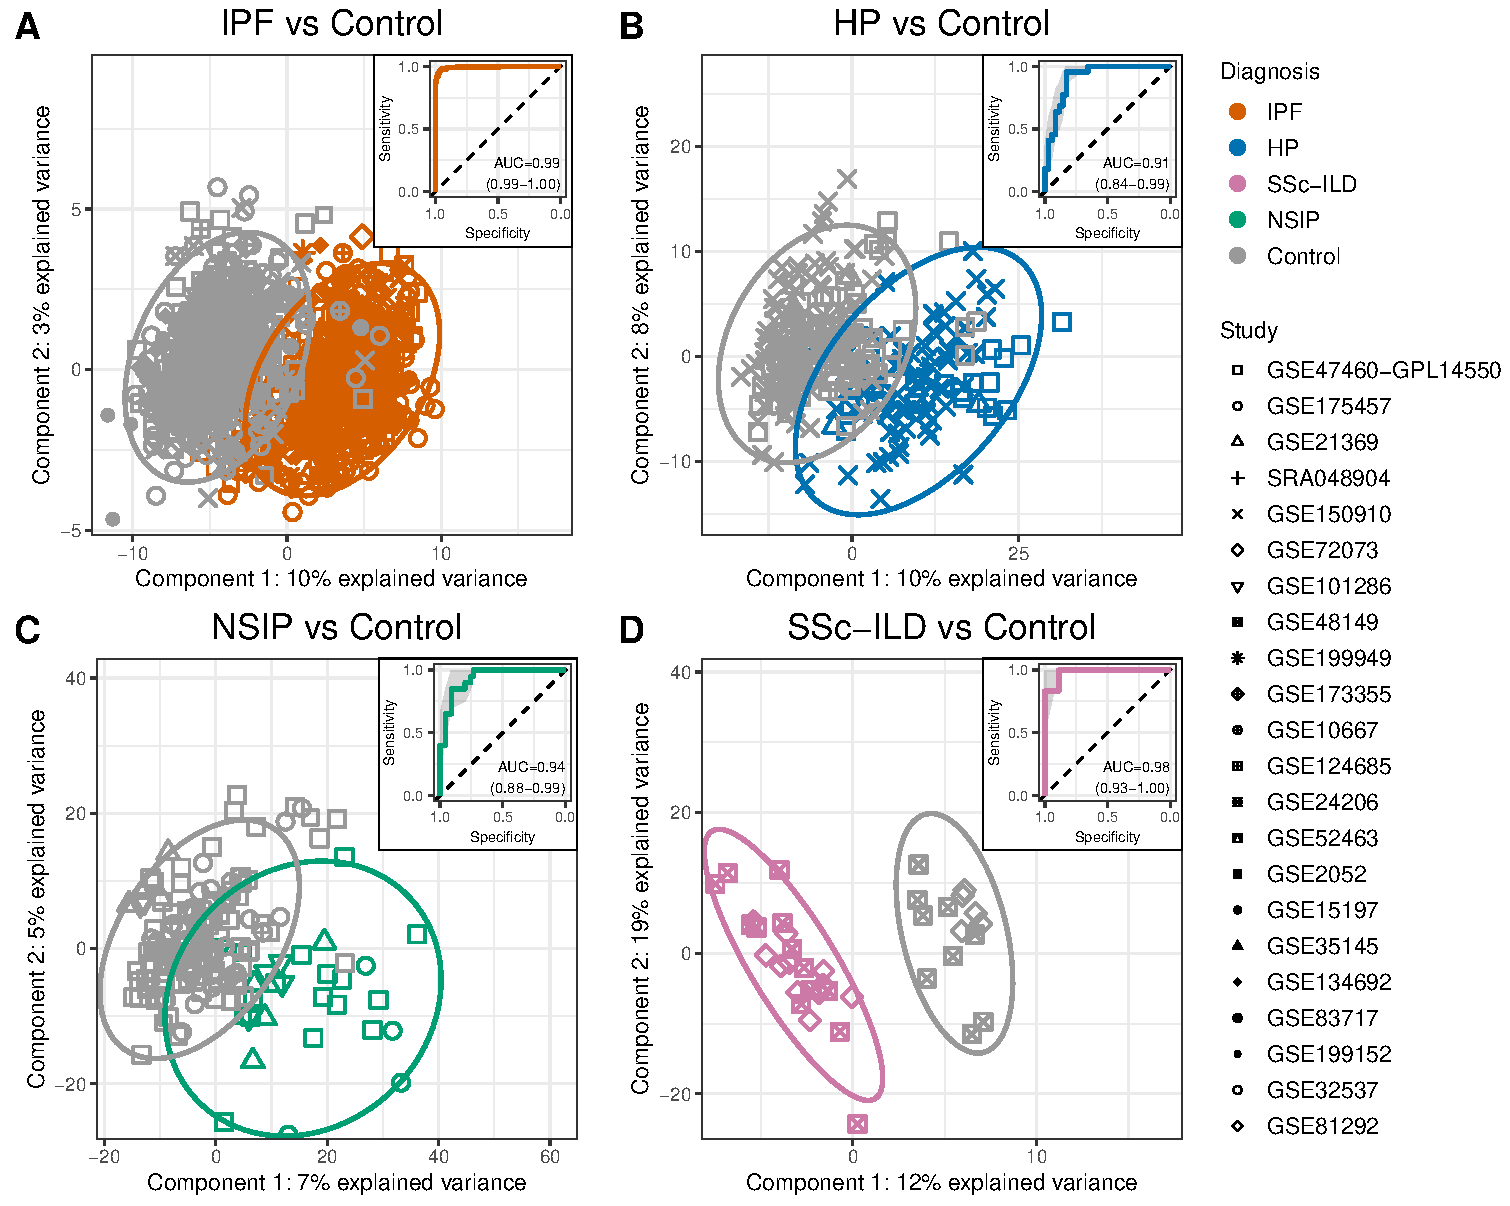
\includegraphics[width=1\linewidth,]{./Figures/SysReview/Figure3_MINT} 

}

\caption[MINT models]{\textbf{Classification models for ILD subtypes against controls.} Training set datasets were integrated and tuned to develop classification models, which were then validated on test set datasets. Projection of MINT-integrated training set samples into the space of the first two PLS components for IPF (A), HP (B), SSc-ILD (C), and NSIP (D) classification models. Inset: AUC performance of each ILD classification model on held-out test datasets. Detailed performance metrics for each dataset can be found in Table \ref{tab:modelPerf}.}\label{fig:mintmodel}
\end{figure}

\hypertarget{fibrotic-ild-subtypes-are-differentiated-at-the-transcriptional-level}{%
\subsubsection{Fibrotic ILD subtypes are differentiated at the transcriptional level}\label{fibrotic-ild-subtypes-are-differentiated-at-the-transcriptional-level}}

To examine unique features of fibrotic ILD subtypes at the transcriptional level, we generated classification models for IPF, HP, and NSIP against all other ILD subtypes. Our training set consisted of 721 IPF, 104 HP, 29 NSIP, 24 SSc-ILD, 14 RB-ILD, 14 unknown fibrosis, six COP, four DIP, three rheumatoid arthritis-ILD (RA-ILD), and one CTD-ILD samples, while our test set consisted of 193 IPF, 22 HP, 20 NSIP, six SSc-ILD, five mixed IPF-NSIP, three unknown fibrosis, two RB-ILD, two DIP, two CTD-ILD, one COP, and one combined pulmonary fibrosis and emphysema (CPFE) samples. The 57-gene IPF vs ILD model trained on seven datasets had good performance on six test datasets (AUC=0.71 {[}0.63-0.79{]}), as did the 132-gene HP vs ILD model trained on three datasets on two test datasets (AUC=0.76 {[}0.63-0.89{]}) (Figure \ref{fig:ILDvILD}, Table \ref{tab:ipfnongenes}, Table \ref{tab:hpnongenes}). The NSIP vs ILD model trained on five datasets did not have a good performance on four test datasets (AUC=0.60 {[}0.49-0.72{]}) (Figure \ref{fig:nsipmodel}). For between-subtype comparisons, we identified a 95-gene signature differentiating IPF from HP samples (AUC=0.76 {[}0.64-0.87{]} on three test datasets), as well as a 67-gene signature differentiating IPF from NSIP samples (AUC=0.76 {[}0.64-0.88{]} on four test datasets) (Figure \ref{fig:ildvsildspecific}A-D, Table \ref{tab:ipfhpgenes}, Table \ref{tab:ipfnsipgenes}). A classifier differentiating HP from NSIP had variable performance on 2 test datasets (AUC=0.74 {[}0.51-0.96{]}) (Figure \ref{fig:ildvsildspecific}E-F, Table \ref{tab:hpnsipgenes}).



\begin{figure}

{\centering 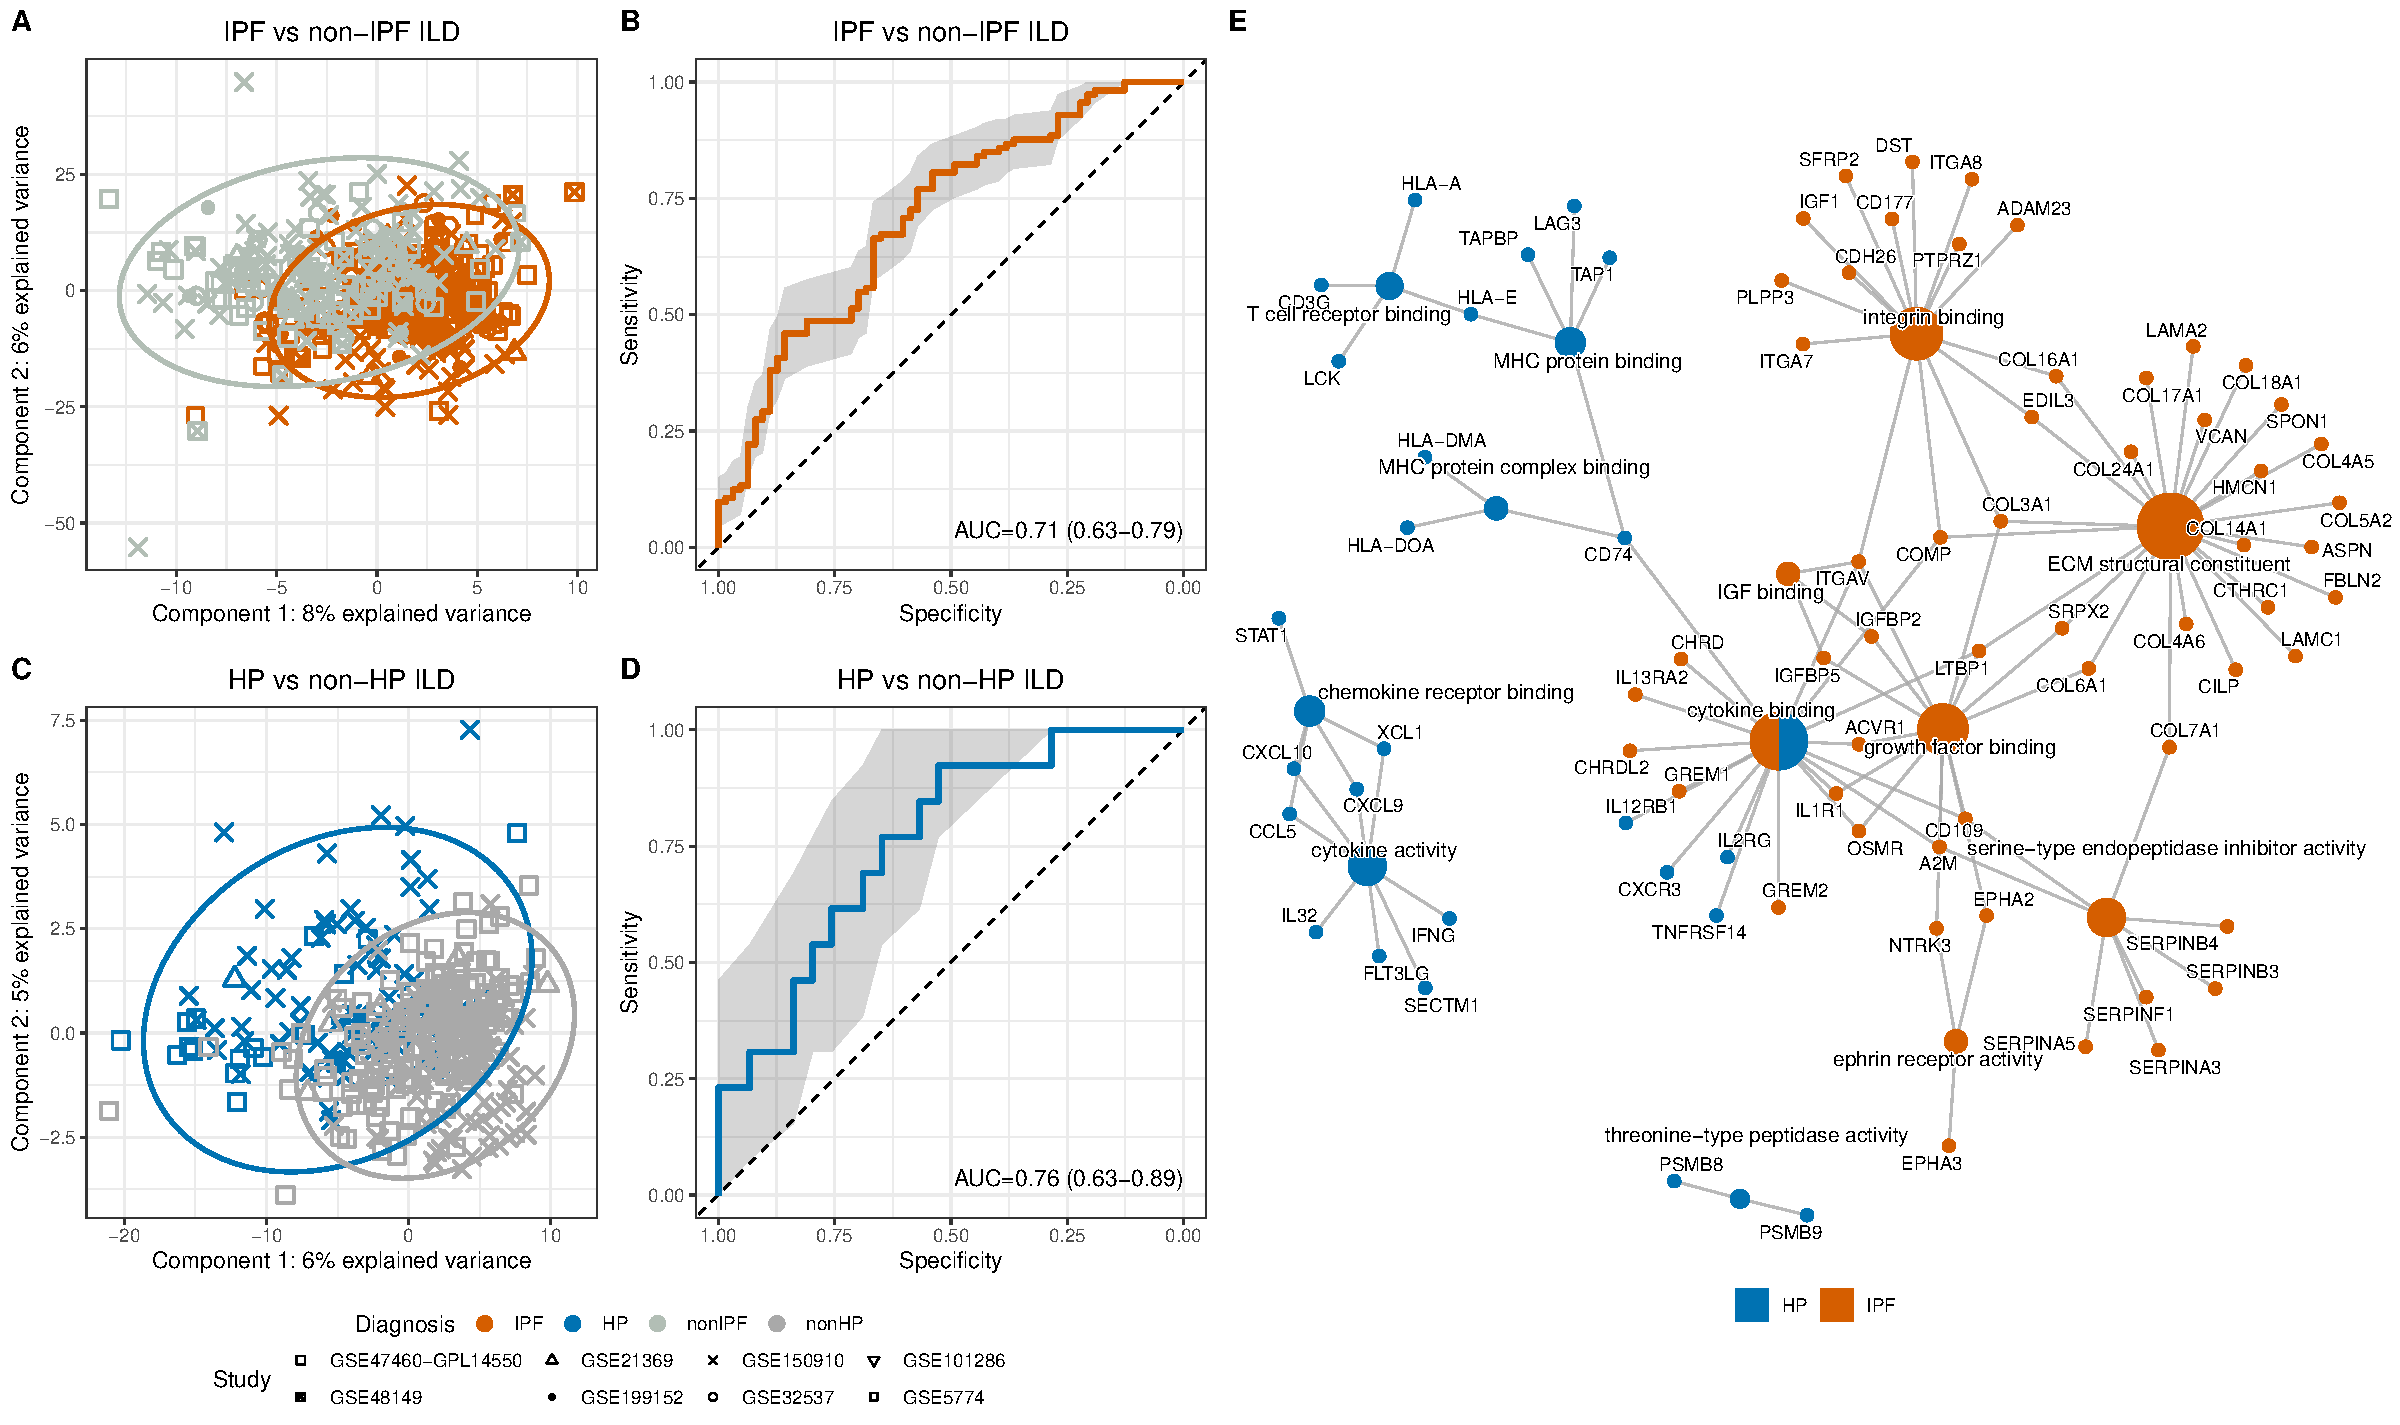
\includegraphics[width=0.95\linewidth,]{./Figures/SysReview/Figure4_ILDvsILD} 

}

\caption[ILD vs ILD]{\textbf{ILD subtype-specific classification models.} IPF-specific and HP-specific classification models were developed through MINT integration of lung transcriptomics datasets. MINT-PLS projection of samples for classification models of IPF vs non-IPF ILD (A) and HP vs non-HP ILD (C), with corresponding performance on held-out test datasets (B, D). Upregulated pathways using gene signatures identified in classification models for IPF against non-IPF ILD and HP against non-HP ILD are shown in (E).}\label{fig:ILDvILD}
\end{figure}

\hypertarget{ild-subtypes-have-both-common-and-unique-disease-pathways}{%
\subsubsection{ILD subtypes have both common and unique disease pathways}\label{ild-subtypes-have-both-common-and-unique-disease-pathways}}

As the ILD classification models had few genes for pathway analysis, we generated ``expanded'' classification models with an increased number of genes using Bayesian changepoint analysis and verified their discrimination ability using the same test sets (Figure \ref{fig:bayes}, Tables \ref{tab:uppathways}-\ref{tab:downpathways}). Using the expanded gene signatures of ILD subtypes against controls, we identified \textit{MMP7}, \textit{COMP}, \textit{DIO2}, \textit{THBS4}, \textit{IL13RA2}, \textit{MEOX1}, \textit{COL17A1}, and \textit{SCG5} as shared upregulated genes across all subtypes when compared against controls (Figure \ref{fig:ILDpathways}A, Figure \ref{fig:modelUpset}C). With reference to the MSigDB C8 collection, these genes are primarily expressed by aberrant basaloid and basal cells (Figure \ref{fig:ILDpathways}C, Table \ref{tab:upcell}). Shared downregulated genes suggested a decrease in AT1 (\textit{MYRF}, \textit{AGER}) and endothelial (\textit{CA4}, \textit{PRX}, \textit{VIPR1}) cells (Figure \ref{fig:ILDpathways}B, Figure \ref{fig:modelUpset}D, Table \ref{tab:downcell}). No `IPF vs Control' lung gene signatures were shared with peripheral signatures; however, blood and PBMC gene signatures shared 21 genes (Figure \ref{fig:modelUpset}B).



\begin{figure}

{\centering 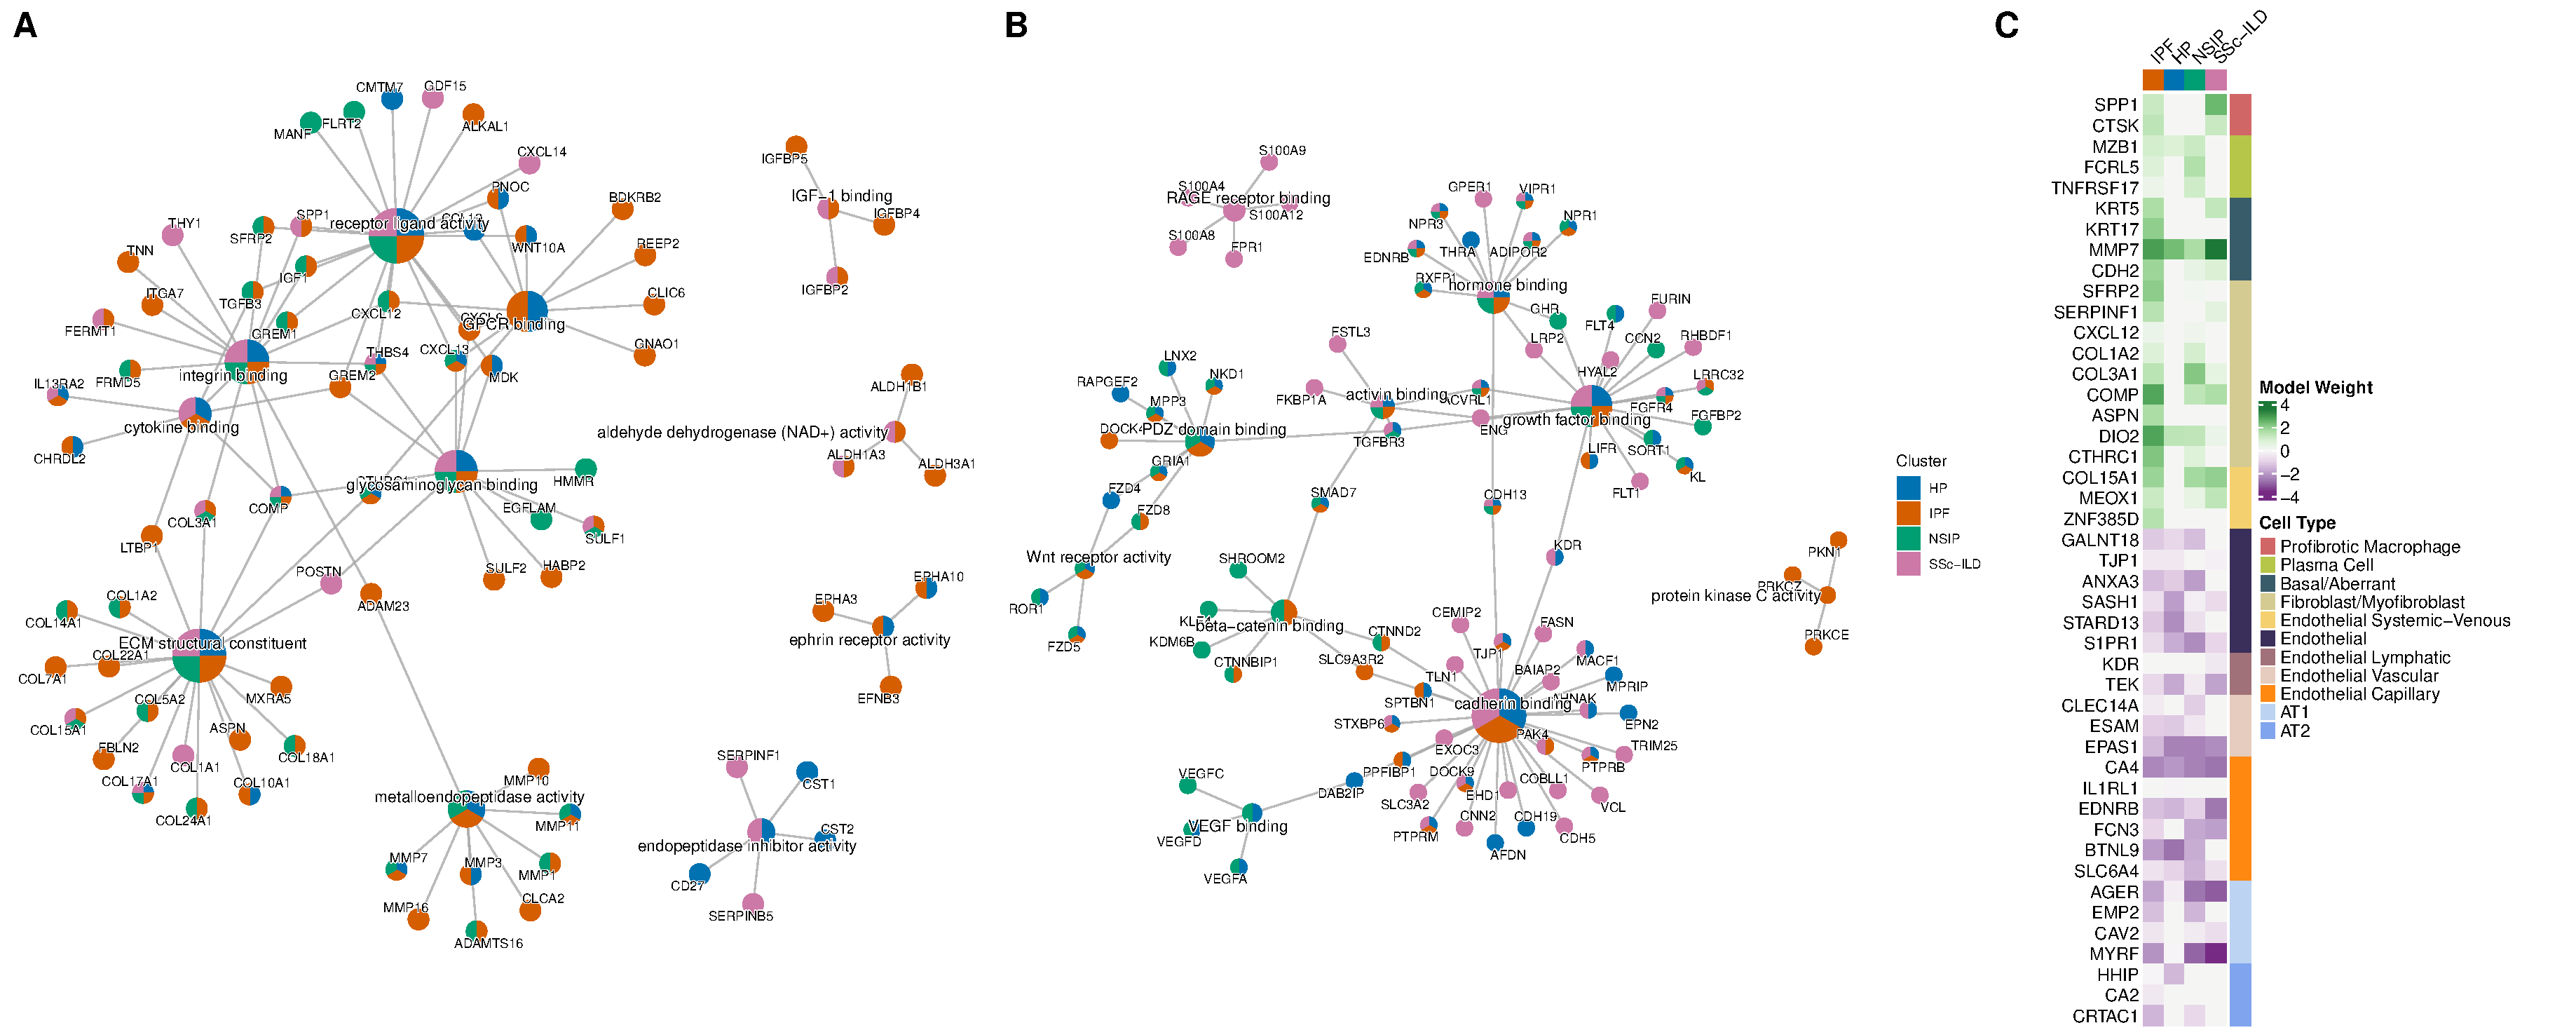
\includegraphics[width=1\linewidth,]{./Figures/SysReview/Figure5_pathways} 

}

\caption[ILD pathways]{\textbf{Pathway analysis of gene signatures from classification models of ILD subtypes against control.} Using up- (A) and down-regulated (B) gene signatures from each ILD classification model, overrepresentation analysis of gene ontology (GO) terms was performed and visualized as a gene-concept network plot. (C) A heatmap of model weights for selected gene markers associated with single-cell marker annotations identified in ILD scRNA-seq analysis (see Data Supplement).}\label{fig:ILDpathways}
\end{figure}

We identified \textit{GPSM2}, \textit{HSPA4L} (previously shown to be involved in the differentiation of AT2 cells {[}\protect\hyperlink{ref-mohamed_respiratory_2014}{89}{]}), and ECM-related genes such as \textit{COL16A1}, \textit{ITGA7}, and \textit{VCAN} as uniquely upregulated in IPF compared to other ILD subtypes (Table \ref{tab:ipfvsildpathways}). In HP, we identified antigen presentation and major histocompatibility complex (MHC) binding as enriched pathways via \textit{PSMB8}, \textit{PSMB9}, and \textit{TAPBP} expression (Figure \ref{fig:ILDvILD}E, Table \ref{tab:hpvsildpathways}), and these genes were also included in the models differentiating HP from IPF and NSIP samples. SSc-ILD samples were uniquely characterized by expression of \textit{CDH3}, which encodes E-cadherin and was not found to be upregulated in signatures of other fibrotic ILD subtypes.

\hypertarget{unsupervised-analysis-identifies-putative-molecular-endotypes-of-ild}{%
\subsubsection{Unsupervised analysis identifies putative molecular endotypes of ILD}\label{unsupervised-analysis-identifies-putative-molecular-endotypes-of-ild}}

We next used biclustering, an unsupervised learning method, to examine transcriptomic lung samples for specific molecular endotypes. Biclustering algorithms perform simultaneous clustering of rows (genes) and columns (samples) of a data matrix to identify subsets known as biclusters {[}\protect\hyperlink{ref-rose_mosbi_2022}{52}{]}. We used a series of biclustering algorithms on our batch-corrected concatenated lung gene expression data to identify 16 biclusters showing enrichment in specific lung disease groups (Figure \ref{fig:biclusterall}, Figure \ref{fig:biclusterjaccard}, Table \ref{tab:biclusterGenes}). Pathway analysis of bicluster genes revealed associations with lung cell types and fibrosis, and top results were used to annotate each bicluster (Table \ref{tab:biclusterPathways}, Figure \ref{fig:biclust}A,B). Of the samples with available predicted FVC\% and DLCO\% data, we identified IPF samples in the `M13-Proliferation' bicluster (n=53) as having lower FVC\% compared to non-cluster (n=155) IPF samples (-6.29\%, FDR=0.09) (Figure \ref{fig:biclust}C, Table \ref{tab:biclusterIPF}), which was not due to age (-1.18 years, \textit{p}=0.15). ILD samples in the `U4-AT1 cells', `U0-Endothelium', `M2-Cytoskeleton', `U1-EMT', `M9-Fibrosis', and `M13-Proliferation' biclusters had significantly lower DLCO\% (-7.95 to -13.9\%, all FDR\textless0.05) compared to non-cluster samples, though these samples were all significantly older with the exception of the `M13-Proliferation' samples which were younger (-2.18 years, FDR=9.17×10\textsuperscript{-3}) (Table \ref{tab:biclusterILD}).



\begin{figure}

{\centering 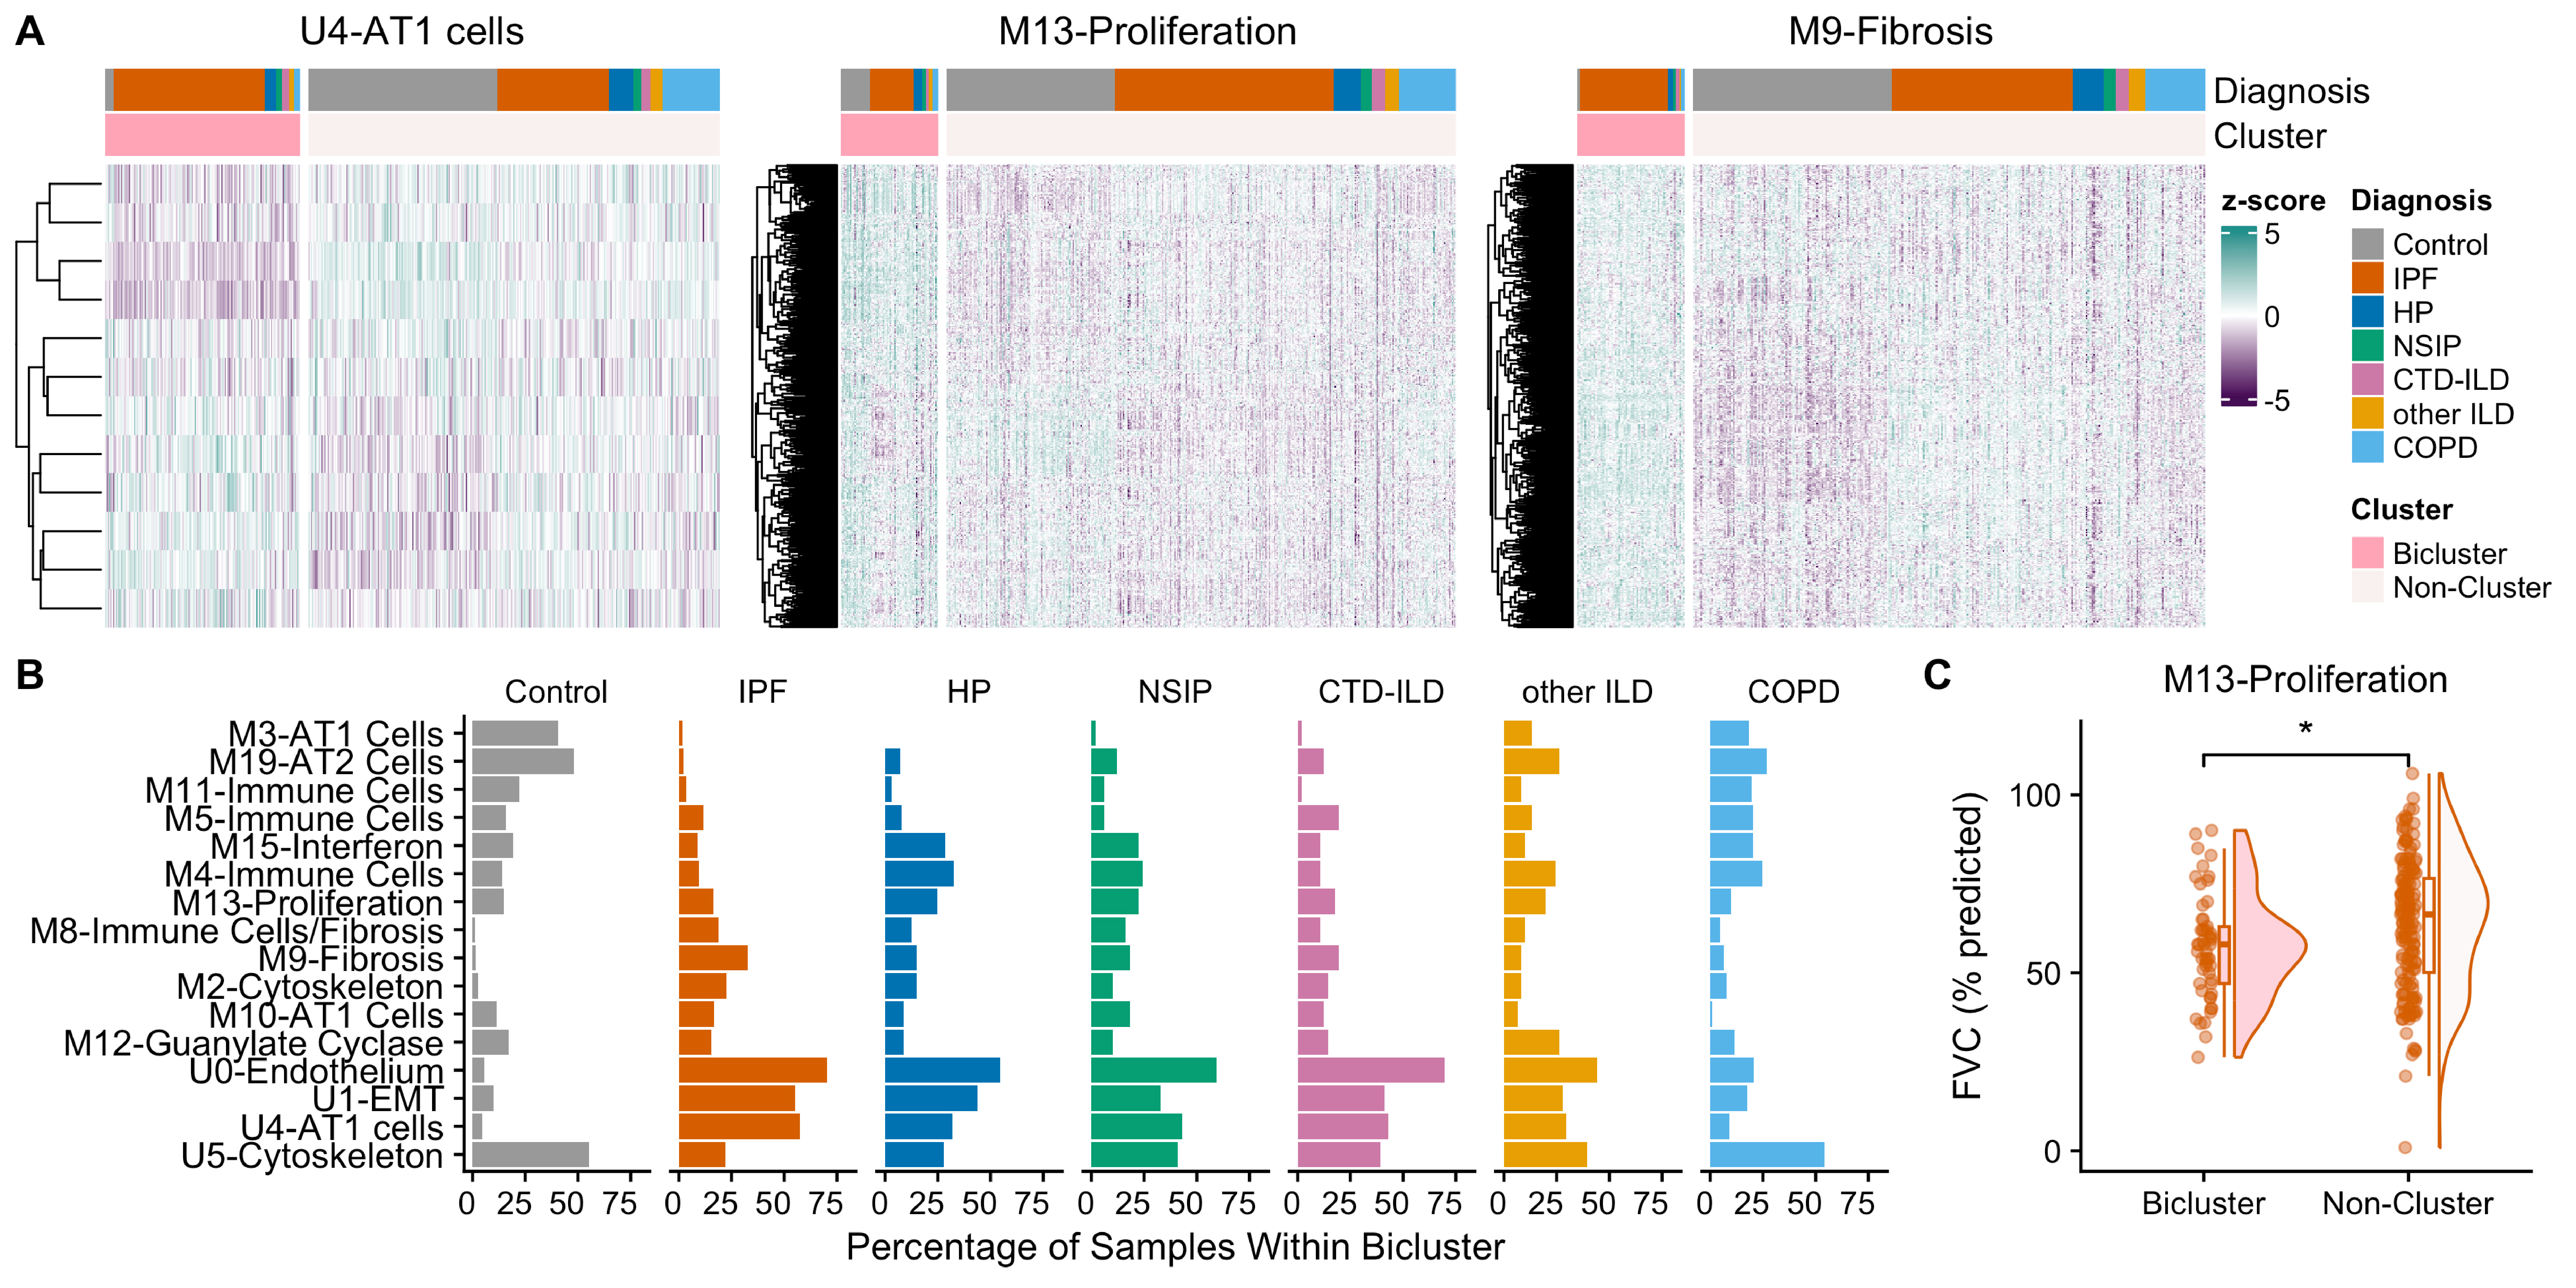
\includegraphics[width=1\linewidth,]{./Figures/SysReview/Figure6_biclusters} 

}

\caption[ILD pathways]{\textbf{Biclusters identified by unsupervised learning.} ComBat-corrected lung transcriptomics datasets containing Control, ILD, and COPD samples were analyzed using biclustering algorithms. (A) Heatmaps of genes found in select biclusters showing differences in gene expression between bicluster and non-bicluster samples. (B) Proportion of samples within each subtype identified in each bicluster (i.e.~32.6\% of IPF samples are in the M9-Fibrosis bicluster). (C) Comparison of reported predicted forced vital capacity (FVC\%) in IPF samples within and outside of the `M13-Proliferation' bicluster. Significance was determined through linear regression analysis of bicluster membership against FVC\% (*, FDR\textless0.10).}\label{fig:biclust}
\end{figure}

\hypertarget{discussion}{%
\subsection{Discussion}\label{discussion}}

ILDs arise as a result of complex interactions between aging, genetics, and environmental factors, with these complex drivers of ILD reflected in their lung transcriptomics. We identified fibrotic ILD subtype-specific gene signatures in the largest meta-analysis of fibrotic ILD transcriptomics to date comprising 1,767 samples, and performed the first comprehensive transcriptomics analysis of fibrotic ILD subtypes against other ILD subtypes to identify candidate subtype-specific biomarkers and molecular endotypes of ILD. Our selected method of integration does not require batch correction of training sets with test sets or a particular normalization method prior to sample classification, thereby resulting in an inductive (not transductive) approach that is less prone to overfitting. The identified fibrotic ILD gene signatures (against all ILD subtypes and controls) were validated on three recently published datasets, suggesting that they may be applied to future ILD transcriptomics datasets.

Our sex-stratified analysis suggests there are similarities between females and males in the pathogenesis of ILD, as the majority of our sex-specific models had comparable performance on sex-stratified test sets. Pathway overrepresentation analysis of genes uniquely found in our sex-specific models revealed immune-associated pathways in female classification models. In particular, both female-specific IPF and NSIP vs Control models contained \textit{CD79A}, a B cell marker, which is consistent with females generally having higher B cell numbers and associated gene expression when compared to males {[}\protect\hyperlink{ref-klein_sex_2016}{90}{]}. Previous studies have identified increases in B cells in patients with ILD {[}\protect\hyperlink{ref-herrera_uipipf_2022}{91}--\protect\hyperlink{ref-schiller_deep_2017}{93}{]}, thus warranting further investigations into the role of B cells in ILDs particularly with a focus on potential sex-specific differences.

Genes used in our classification models are representative of ILD pathogenesis. Well-studied genes (e.g.~\textit{MMP7}) and disease processes were up-regulated across all ILD subtypes, which is consistent with the overlapping radiological and pathological morphology, disease progression, and treatment response {[}\protect\hyperlink{ref-flaherty_nintedanib_2019}{19}{]}. Unique genes expressed in IPF were associated with the ECM; in particular, \textit{VCAN}, \textit{SPON1}, and \textit{FBLN2} have been found to be increased in fibroblastic foci of UIP/IPF lungs {[}\protect\hyperlink{ref-herrera_uipipf_2022}{91}{]}. The presence of MHC and antigen presentation-associated genes (\textit{TAPBP}, \textit{PSMB8}, and \textit{PSMB9}) in both HP vs Control and HP vs non-HP models suggests that they may have diagnostic utility as biomarkers as they are overexpressed in HP and have HP-associated haplotypes {[}\protect\hyperlink{ref-camarena_psmb8_2010}{94}{]}. E-cadherin (\textit{CDH3}), which was uniquely identified in the SSc-ILD vs Control model but not in other ILDs, forms a key component of the adherens junction that stabilizes the airway epithelial barrier and its loss of expression has been reported as a hallmark of EMT {[}\protect\hyperlink{ref-bartis_epithelialmesenchymal_2014}{95}{]}. However, we were unable to identify a model for NSIP vs other ILD with good performance on test datasets, which was corroborated by three studies included in our systematic review {[}\protect\hyperlink{ref-cho_systems_2011}{62},\protect\hyperlink{ref-yang_gene_2007}{73},\protect\hyperlink{ref-horimasu_gene_2017}{83}{]}. Given that NSIP is observed in both idiopathic NSIP and many types of CTD-ILD, it is unsurprising that a consensus gene signature is difficult to identify in a heterogenous population.

Through the use of two unsupervised biclustering algorithms, we identified 16 biclusters spanning various mechanisms of ILD including immune infiltration and fibrosis. The `M2-Cytoskeleton' bicluster contained microtubule and dynein (e.g.~\textit{DYNAH7}, \textit{DYNAH9}) genes associated with ciliated cells, which may be associated with microscopic honeycombing seen in IPF/UIP {[}\protect\hyperlink{ref-yang_expression_2013}{65}{]}. Two biclusters, `U4-AT1 cells' and `U0-Endothelium', were annotated due to downregulation of genes associated with AT1 cells (\textit{AGER}, \textit{CAV2}, \textit{EMP2}) and endothelial cells (\textit{EPAS1}, \textit{TEK}, \textit{STARD13}), and destruction of these tissues during the pathogenesis of ILD may explain the association with reduced DLCO\% in ILD samples. The 'M13-Proliferation' bicluster was associated with decreased FVC\% and DLCO\% in all ILD samples, and in IPF patients it was associated with a \textasciitilde6\% decline in FVC\%. Genes contained in this bicluster are involved in the cell cycle, and pathway analysis revealed associations with proliferating macrophages, basal cells, and NK/T cells {[}\protect\hyperlink{ref-travaglini_molecular_2020}{96}{]}; one of the genes, \textit{CCNA2}, has previously been reported as upregulated in acute exacerbations of IPF {[}\protect\hyperlink{ref-konishi_gene_2009}{75}{]}.

Taken together, our supervised and unsupervised analyses suggest that current diagnostic classifications do not fully capture molecular heterogeneity within subtypes. When comparing genes from our expanded IPF vs non-IPF ILD model to the UIP Envisia classifier, only 10/190 genes (\textit{PDLIM5}, \textit{GREM1}, \textit{TUBB2B}, \textit{CHRDL2}, \textit{KIF12}, \textit{SLC4A3}, \textit{PPIC}, \textit{ZNF454}, \textit{SELE}, \textit{MYO3B}) were shared (Figure \ref{fig:envisia}), which might be explained by UIP patterns being observed in other fibrotic ILDs such as RA-ILD as well as IPF diagnoses not being limited to UIP patterns. While our classification models perform well in separating IPF or HP from other ILDs, it is evident from the unsupervised analysis that there exists molecular heterogeneity within these subtypes, and these putative endotypes are associated with lung function. Considering the complex drivers and heterogenous presentations of ILD subtypes, future classification based on data-driven molecular endotypes may be clinically beneficial with respect to disease management as well as research and development into novel therapeutics.

Our analysis is limited by the lack of detailed patient-level secondary data. Although patients in the LTRC are well-phenotyped, variables such as radiological pattern, age, treatment status, pulmonary function tests, disease staging, and mortality were often reported as summary tables, thereby prohibiting detailed subgroup analyses. However, using available metadata, we were able to examine age (n=852), predicted FVC\% (n=309), and predicted DLCO\% (n=259) from ILD samples in our unsupervised analysis. Future work in fibrotic ILD transcriptomics should consider the investigation of less profiled subtypes to enrich our understanding of non-IPF pulmonary fibrosis, as the overrepresentation of IPF in our analysis limits the generalizability of our findings. Finally, prediction thresholds in MINT are based upon minimum sample distance to class centroids within the PLS projection space, thus making direct comparison to existing classifiers difficult. Nevertheless, our models had good AUCs and BERs on held-out datasets, providing more confidence in their discriminatory ability and biological relevance to ILD pathobiology.

In summary, by using both supervised and unsupervised approaches, our meta-analysis has identified reproducible fibrotic ILD subtype-specific gene signatures and molecular endotypes of ILD that reflect the pathogenesis of fibrotic lung disease. Using gene expression profiling, we have developed preliminary classifiers that distinguish individual fibrotic ILD subtypes from each other. Further studies are required to investigate the utility of the herein identified gene signatures and molecular endotypes in a clinical setting.

\clearpage

\hypertarget{diagnostic-potential-of-genomic-blood-biomarkers-of-pulmonary-fibrosis-a-pilot-study}{%
\section{Diagnostic potential of genomic blood biomarkers of pulmonary fibrosis: a pilot study}\label{diagnostic-potential-of-genomic-blood-biomarkers-of-pulmonary-fibrosis-a-pilot-study}}

\renewcommand{\thefigure}{3.\arabic{figure}}
\setcounter{figure}{0}
\renewcommand{\thetable}{3.\arabic{table}}
\setcounter{table}{0}
\renewcommand{\theequation}{3.\arabic{equation}}
\setcounter{equation}{0}

Given the scarcity of disease biomarkers in ILD, investigations into molecular biomarkers of ILD (particularly circulating biomarkers) are an ongoing area of interest {[}\protect\hyperlink{ref-clynick_biomarker_2022}{97}--\protect\hyperlink{ref-bowman_proteomic_2022}{99}{]}. A 52-gene signature derived from PBMC transcriptomic profiling has been shown to be predictive of transplant-free survival in patients with IPF {[}\protect\hyperlink{ref-herazo-maya_peripheral_2013}{59},\protect\hyperlink{ref-herazo-maya_validating_2017}{100}{]}, and transcriptomic profiling has also identified genes associated with decline in lung function in the ILD subtypes IPF and HP {[}\protect\hyperlink{ref-yang_peripheral_2012}{54},\protect\hyperlink{ref-huang_blood_2021}{101},\protect\hyperlink{ref-fernandez_perez_prognostic_2022}{102}{]}.

While it is evident that the peripheral transcriptome is associated with prognosis in ILD, no investigations have been performed regarding its diagnostic potential. The objective of this study was to evaluate the ability of the whole blood transcriptome in discriminating between ILD subtypes. In this pilot study, we profiled whole blood RNA obtained from patients with ILD (n=59) using a previously published NanoString assay designed to discriminate between the early- and late-phase asthmatic response {[}\protect\hyperlink{ref-singh_novel_2018}{103}{]}. Given that fibrosis is a TH2-driven process like asthma {[}\protect\hyperlink{ref-spagnolo_role_2022}{104}{]}, we reasoned that the transcripts profiled in the assay might also differentiate between other TH2-like disease subtypes.

\hypertarget{methods-1}{%
\subsection{Methods}\label{methods-1}}

\hypertarget{study-population-and-sample-processing}{%
\subsubsection{Study population and sample processing}\label{study-population-and-sample-processing}}

Patients were diagnosed with fibrotic ILD (IPF, n=22; HP, n=14; SSc-ILD, n=20; IPAF, n=3) in accordance with diagnostic guidelines and prospectively recruited with written informed consent (ethics protocol H09-00748) between 2012 and 2018 at St.~Paul's Hospital (Vancouver, BC, Canada). At time of sampling, patients were either undergoing anti-fibrotic (pirfenidone, nintedanib), anti-inflammatory (prednisone, mycophenolate, N-acetylcysteine), or no pharmacotherapy. Whole blood samples were collected in PAXgene Blood RNA Tubes (BD Biosciences, Mississauga, ON, Canada) and extracted for RNA using the PAXgene Blood miRNA Kit (PreAnalytiX, Hombrechtikon, Switzerland). RNA quality was confirmed by the RNA 6000 Nano Kit (Agilent, Santa Clara, California, USA) via RNA integrity numbers obtained from Bioanalyzer analysis. Blood transcript expression was profiled using 100 ng of purified RNA with a custom NanoString nCounter Elements assay (NanoString Technologies, Seattle, WA, USA) that measured 166 transcripts {[}\protect\hyperlink{ref-singh_novel_2018}{103}{]}. Samples were randomized across six NanoString cartridges (12 samples per cartridge), with remaining assay slots used for sample replicates to assess data reproducibility.

\hypertarget{in-situ-hybridization}{%
\subsubsection{In situ hybridization}\label{in-situ-hybridization}}

Custom RNAscope™ probes for KLRF1 (276-375 of NM\_016523.1), LTK (2419-2518 of NM\_001135685.1), and VCAN (transcript variant 3; 1356-1455 of uc003kij.3) were developed by Advanced Cell Diagnostics (ACD, Newark, California). Tissue microarray (TMA) sections (4\(\mu\)m-thick) were obtained from a formalin-fixed and paraffin-embedded TMA block containing cores from donor lungs of patients with IPF, HP, and SSc-ILD collected at McMaster University. In situ hybridization (ISH) was performed using a Leica BOND RX autostainer with associated Leica reagent kits (Concord, Ontario, Canada) on TMA sections. Slides were scanned at 40X magnification with an Olympus VS120-L100 Virtual Slide System for image capture and a Leica Aperio ScanScope AT2 for quantification. Image analysis was performed using QuPath (v0.4.3), and probe quantification was determined using H-scores as indicated by manufacturer protocols.

\hypertarget{data-analysis}{%
\subsubsection{Data analysis}\label{data-analysis}}

NanoString data underwent quality assessment by examining field of view (FOV) ratio (number of FOV images successfully captured), binding density (image saturation), linearity of positive controls, and limit of detection via negative controls. Data were filtered for lowly abundant features, then normalized using normalization factors derived from the geometric mean of 10 housekeeping transcripts. Differential expression analysis of transcripts was performed using the linear models for microarray (limma) R package (v3.54.2), while biomarker panels were developed using sparse partial least squares discriminant analysis (sPLSDA), elastic net, and random forest algorithms from the `mixOmics' (v6.22.0) and `tidymodels' (v1.0.0) R packages. Image analysis was performed using QuPath (v0.4.3) by automatically identifying individual cells and setting probe-specific thresholds based on signal strength. Cells without a visible nucleus were excluded from analysis. H-scores were determined by grouping cells into 5 bins based on the numbers of dots per cell (0, 1-3, 4-9, 10-15, \textgreater15) and multiplying the total percentage of cells in each bin by 0 to 4. To test for statistical significance of H-scores, a linear mixed-effects model (`lme4' v1.1-32) was fitted with the formula H-Score \textasciitilde{} Diagnosis + (1\textbar Patient) and pairwise comparisons between diagnoses to determine statistical significance with Tukey's post-hoc adjustment were performed using the `emmeans' (v1.8.5) R package. Fisher's exact test was used to test for differences in demographic count variables between diagnoses, while the F-test was used to test for differences in demographic continuous variables between diagnoses. All analysis was performed in the R (version 4.2.3) statistical computing environment.

\hypertarget{results-1}{%
\subsection{Results}\label{results-1}}

We profiled the expression of 166 RNA transcripts in a cohort of patients with IPF, systemic sclerosis-associated ILD (SSc-ILD), HP, or interstitial pneumonia with autoimmune features (IPAF) (Table \ref{tab:bloodpx}). No significant differences were identified between subtypes for race, percent predicted forced vital capacity (FVC\%) or diffusing capacity of the lung for carbon monoxide (DLCO\%), smoking status, or treatment status, but patients with SSc-ILD and IPAF were younger at time of sampling and patients with IPF were predominantly male which is in line with previously reported cohorts {[}\protect\hyperlink{ref-zaman_differences_2020}{105}{]}.

\captionsetup{width=6.5in}





\begin{table}[!h]
\centering\centering
\caption{\label{tab:bloodpx}\textbf{Summary table of clinical demographics of patients probed for whole blood RNA expression.}}
\centering
\begin{tabu} to \linewidth {>{\raggedright\arraybackslash}p{1.3in}>{\centering\arraybackslash}p{0.9in}>{\centering\arraybackslash}p{1.0in}>{\centering\arraybackslash}p{0.9in}>{\centering\arraybackslash}p{0.9in}>{\centering\arraybackslash}p{0.75in}}
\toprule
 & IPF (n=22) & SSc-ILD (n=20) & HP (n=14) & IPAF (n=3) & \textit{p}-value\\
\midrule
Male sex, n (\%) & 17 (77) & 2 (10) & 5 (36) & 1 (33) & \textit{p} < 0.0001\\
Age, mean ± SD & 69.91 ± 7.31 & 60.85 ± 9.12 & 66.21 ± 7.26 & 56.00 ± 7.81 & \textit{p} = 0.0014\\
FVC\% mean ± SD & 74.18 ± 15.29 & 83.10 ± 18.07 & 70.21 ± 16.30 & 72.67 ± 20.50 & \textit{p} = 0.1435\\
DLCO\%, mean ± SD & 42.41 ± 11.79 & 54.70 ± 19.46 & 45.00 ± 13.21 & 52.00 ± 5.20 & \textit{p} = 0.0624\\
Ever smoked, n (\%) & 16 (80) & 12 (60) & 7 (50) & 2 (67) & \textit{p} = 0.2780\\
\midrule
Race, n (\%) &  &  &  &  & \textit{p} = 0.6358\\
Asian & 2 (9) & 4 (20) & 1 (7) & 1 (33) & \\
American Indian & 1 (5) & 0 (0) & 0 (0) & 0 (0) & \\
Pacific Islander & 1 (5) & 0 (0) & 1 (7) & 0 (0) & \\
White & 18 (82) & 16 (80) & 12 (86) & 2 (67) & \\
\midrule
Treatment, n (\%) &  &  &  &  & \textit{p} = 0.6981\\
Anti-Fibrotic & 9 (41) & 0 (0) & 0 (0) & 0 (0) & \\
Anti-Inflammatory & 0 (0) & 11 (55) & 9 (64) & 2 (67) & \\
Anti-Fibrotic and Anti-Inflammatory & 1 (5) & 0 (0) & 0 (0) & 0 (0) & \\
None & 12 (55) & 9 (45) & 5 (36) & 1 (33) & \\
\bottomrule
\end{tabu}
\end{table}

To identify variables that might affect RNA expression, we performed a principal component (PC) analysis and correlated the PCs with demographic variables (\ref{fig:pilotPCA}). After adjusting for race and treatment status, we identified 1 differentially expressed transcript at an FDR of 0.05 when comparing IPF to SSc-ILD (\textit{KLRF1}, FDR = 0.03) (Table \ref{tab:pilotdiffexp}, Figure \ref{fig:pilotexpr}D). While no transcripts were significantly associated with FVC\%, we identified 13 transcripts that were significantly associated with DLCO\% (Table \ref{tab:pilotpftdeg}). Next, we examined the utility of RNA profiling in developing biomarker panels to differentiate between ILD subtypes through the use of three learning algorithms (sparse partial least squares discriminant analysis (sPLSDA), elastic net, and random forest). The best-performing models using 5-fold cross-validation repeated ten times were IPF vs SSc-ILD (sPLSDA) and IPF vs SSc-ILD (elastic net), which yielded respective accuracies of 0.74 ± 0.01 and 0.80 ± 0.02 (Table \ref{tab:biomarkermodel}).

\newpage

\captionsetup{width=6.5in}

\begin{singlespace}








\begin{table}[!h]
\centering\centering
\caption{\label{tab:pilotdiffexp}\textbf{List of transcripts analyzed for differential expression between ILD subtypes.} Results shown are adjusted for using treatment status and race. }
\centering
\begin{tabu} to \linewidth {>{\raggedright\arraybackslash}p{1.3in}>{\centering\arraybackslash}p{0.7in}>{\centering\arraybackslash}p{0.7in}>{\centering\arraybackslash}p{0.7in}}
\toprule
Transcript & log\textsubscript{2}FC & \textit{p}-value & FDR\\
\midrule
\textbf{IPF vs non-IPF} &  &  & \\
VCAN\_isoform & 0.38 & 0.01 & 0.93\\
KLRF1 & 0.27 & 0.02 & 0.93\\
LTK & -0.22 & 0.02 & 0.93\\
CFD & 0.52 & 0.02 & 0.93\\
C3AR1 & 0.20 & 0.07 & 1.00\\
\textbf{IPF vs SSc-ILD} &  &  & \\
KLRF1 & 0.46 & 0.00 & 0.03\\
GNLY & 0.76 & 0.01 & 0.56\\
CMC1 & 0.28 & 0.02 & 0.85\\
LMBRD1 & -0.19 & 0.04 & 0.99\\
LTK & -0.22 & 0.04 & 0.99\\
\textbf{IPF vs HP} &  &  & \\
CFD & 0.73 & 0.01 & 0.99\\
LTK & -0.25 & 0.04 & 0.99\\
STAT6 & 0.18 & 0.06 & 0.99\\
VCAN\_isoform & 0.36 & 0.06 & 0.99\\
PLXNC1\_isoform & 0.29 & 0.07 & 0.99\\
\textbf{HP vs SSc-ILD} &  &  & \\
KLRF1 & 0.45 & 0.00 & 0.16\\
RORC & -0.50 & 0.00 & 0.16\\
GNLY & 0.79 & 0.01 & 0.48\\
FCGR3A & -0.52 & 0.01 & 0.48\\
CMC1 & 0.29 & 0.03 & 0.81\\
\bottomrule
\end{tabu}
\end{table}

\end{singlespace}

To investigate the lung expression of the three most highly weighted genes (\textit{KLRF1}, \textit{LTK}, \textit{VCAN}) identified by our blood biomarker panels when comparing IPF vs non-IPF ILD (Table \ref{tab:biomarkerweight}), we used ISH on TMA sections consisting of twelve cores from five patients with IPF, ten cores from three patients with HP, and four cores from two patients with SSc-ILD (Figure \ref{fig:pilotexpr}A-C), all of which showed no between-group differences in demographic or clinical variables (Table \ref{tab:lungpx}). Transcript abundance was determined semi-quantitatively for each marker per core by calculating H-scores, which is a weighted total of cells expressing the probe. Using a linear mixed-effects analysis, the H-score of \textit{KLRF1} was higher in SSc-ILD compared to IPF (\textit{p}=0.02) and HP (\textit{p}=0.01), while \textit{LTK} was lower in IPF compared to SSc-ILD (\textit{p}=0.03) (Figure \ref{fig:pilotexpr}).

\captionsetup{width=6.5in}



\begin{table}[!h]
\centering\centering
\caption{\label{tab:lungpx}\textbf{Summary table of clinical demographics of patients probed for \textit{LTK}, \textit{KLRF1}, and \textit{VCAN} expression using in situ hybrdization in lung tissue microarray sections.}}
\centering
\begin{tabu} to \linewidth {>{\raggedright\arraybackslash}p{1.3in}>{\centering\arraybackslash}p{1.0in}>{\centering\arraybackslash}p{1.0in}>{\centering\arraybackslash}p{1.0in}>{\raggedright\arraybackslash}p{1.0in}}
\toprule
 & IPF (n=5) & HP (n=3) & SSc-ILD (n=2) & \textit{p}-value\\
\midrule
Female sex, n (\%) & 4 (80) & 3 (100) & 1 (50) & \textit{p} = 0.2222\\
Age, mean ± SD & 59.40 ± 9.32 & 59.67 ± 10.79 & 62.00 ± 9.90 & \textit{p} = 0.9182\\
FVC\%, mean ± SD & 52.00 ± 12.81 & 72.67 ± 5.13 & 1; 80.00 ± NA & \textit{p} = 0.3523\\
Ever smoked, n (\%) & 2 (40) & 2 (67) & 1 (50) & \textit{p} = 0.7143\\
\bottomrule
\end{tabu}
\end{table}



\begin{figure}

{\centering \includegraphics[width=0.9\linewidth,]{./Figures/BloodPilot/ILD_biomarkers_combined_thesis_v1} 

}

\caption[Blood and Lung expression of LTK, KLRF1, VCAN]{\textbf{Expression of \textit{KLRF1}, \textit{LTK}, \textit{VCAN} in whole blood (log2 RNA expression) or lung tissue microarray sections (H-Score) containing samples from patients with ILD subtypes.} Tissue microarray sections of lung samples from patients with (A) idiopathic pulmonary fibrosis (IPF), (B) hypersensitivity pneumonitis (HP), and (C) systemic sclerosis-associated interstitial lung disease (SSc-ILD). (D) Whole blood (log2 RNA expression) and lung (H-Score) expression of \textit{KLRF1}, \textit{LTK}, and \textit{VCAN}. Statistical significance of blood RNA expression was corrected using false discovery rate (FDR), with significance indicated by FDR\textless0.05 (***). Tukey's post-hoc adjustment was used to determine statistical significance of H-scores (* denotes \textit{p}\textless0.05).}\label{fig:pilotexpr}
\end{figure}

\hypertarget{discussion-1}{%
\subsection{Discussion}\label{discussion-1}}

Although previous studies have investigated the peripheral transcriptome in relation to prognosis {[}\protect\hyperlink{ref-yang_peripheral_2012}{54},\protect\hyperlink{ref-herazo-maya_peripheral_2013}{59},\protect\hyperlink{ref-fernandez_perez_prognostic_2022}{102}{]}, no study has looked at its diagnostic potential. In this pilot study, we demonstrate that the peripheral blood RNA can differentiate between ILD subtypes, in particular IPF and SSc-ILD, through differential expression and learning algorithms utilizing gene expression data obtained from a custom NanoString assay. The blood gene expression data show association with DLCO\% predicted but not FVC\% predicted, which was previously noted when examining differential expression of the peripheral transcriptome in mild and severe IPF {[}\protect\hyperlink{ref-yang_peripheral_2012}{54}{]}. Furthermore, we identify \textit{KLRF1} expression as a significant in the differentiation of IPF and SSc-ILD in both whole blood and lung, and down-regulation of \textit{LTK} as being associated with IPF.

Killer cell lectin like receptor F1 (KLRF1, also known as NKp80) is expressed in T cells, monocytes, and CD56bright natural killer (NK cells), and is a marker of NK cell maturity {[}\protect\hyperlink{ref-roda-navarro_human_2000}{106}--\protect\hyperlink{ref-mukherjee_klrf1_2023}{108}{]}, inducing cytotoxic activity and calcium mobilization {[}\protect\hyperlink{ref-vitale_identification_2001}{109}{]}. The dysfunction of NK cells in systemic sclerosis and autoimmunity has been well-documented {[}\protect\hyperlink{ref-horikawa_abnormal_2005}{110}--\protect\hyperlink{ref-liu_nk_2021}{112}{]}, and differences in their abundance have been observed between ILD subtypes {[}\protect\hyperlink{ref-esposito_natural_2005}{113},\protect\hyperlink{ref-bergantini_prognostic_2021}{114}{]}. We found that \textit{KLRF1} expression was associated with lower DLCO\%, and its expression was lower in the peripheral blood of patients with SSc-ILD compared to IPF and HP yet the opposite effect was observed when probing lung expression. Previous reports have identified a reduction in abundance and function of NK cells in IPF lungs concurrent with an increase in abundance in blood compared to healthy controls {[}\protect\hyperlink{ref-cruz_reduced_2021}{115}{]}. Single-cell RNA-sequencing data available via the IPF Cell Atlas {[}\protect\hyperlink{ref-neumark_idiopathic_2020}{116}{]} suggests higher \textit{KLRF1} expression in SSc-ILD T/NK subsets compared to other ILDs. Given the disparity between single-cell and bulk RNA data, further investigations are required to delineate the mechanisms surrounding NK cell recruitment to the ILD lung and its role in ILD pathogenesis.

\textit{LTK} and \textit{VCAN} were differentially expressed at a nominal p-value of 0.05 between IPF and non-IPF ILDs (but not at FDR\textless0.05), and were two highly weighted coefficients in our elastic net and sPLSDA biomarker panels. \textit{LTK} is highly expressed in plasmacytoid dendritic cells (pDCs) (Human Protein Atlas, IPF Cell Atlas), and decreased circulating pDCs have been reported in IPF patients {[}\protect\hyperlink{ref-galati_circulating_2020}{117}{]}, which is consistent with the decreased \textit{LTK} expression observed in this study in blood and lung. \textit{VCAN} encodes for versican, an ECM proteoglycan that is localized to fibroblastic foci in the lung, myofibroblasts, and monocytes {[}\protect\hyperlink{ref-neumark_idiopathic_2020}{116},\protect\hyperlink{ref-bensadoun_proteoglycan_1996}{118}{]}. We were unable to identify a statistically significant increase in \textit{VCAN} expression in IPF compared to HP or SSc-ILD lung and blood samples; however, given its detectable expression in both lung and peripheral blood, and prior studies showing circulating levels of versican degradation products are associated with increased mortality in idiopathic ILDs {[}\protect\hyperlink{ref-sand_serological_2018}{119}{]}, further studies into its gene expression as a prognostic biomarker may be warranted.

In this pilot study, we report the first between-subtype comparison of the peripheral ILD transcriptome using a discrete set of genes, which validates performing more extensive genome-wide analysis of peripheral ILD subtype-specific profiles and correlations of identified biomarkers in lung tissue. In particular, molecules detected in the blood that are associated with immunity and fibrosis are detectable in the lung, thereby suggesting a test based on peripheral transcriptomics is feasible for diagnostic biomarkers with biological relevance, similar to prognostic markers in Herazo-Maya et al. {[}\protect\hyperlink{ref-herazo-maya_validating_2017}{100}{]}. Using the data from this preliminary pilot study, we were able to secure funding for two grants (BC Lung, Genome BC) that created the basis for the following two chapters.

\clearpage

\hypertarget{genomic-blood-biomarkers-in-ild}{%
\section{Genomic blood biomarkers in ILD}\label{genomic-blood-biomarkers-in-ild}}

\renewcommand{\thefigure}{4.\arabic{figure}}
\setcounter{figure}{0}
\renewcommand{\thetable}{4.\arabic{table}}
\setcounter{table}{0}
\renewcommand{\theequation}{4.\arabic{equation}}
\setcounter{equation}{0}

\clearpage

\hypertarget{insert-title-of-chapter-5-here}{%
\section{Insert Title of Chapter 5 Here}\label{insert-title-of-chapter-5-here}}

\renewcommand{\thefigure}{5.\arabic{figure}}
\setcounter{figure}{0}
\renewcommand{\thetable}{5.\arabic{table}}
\setcounter{table}{0}
\renewcommand{\theequation}{5.\arabic{equation}}
\setcounter{equation}{0}

\clearpage

\hypertarget{conclusion}{%
\section{Conclusion}\label{conclusion}}

Lorem ipsum dolor sit amet, consectetur adipiscing elit. Cras id nulla malesuada, auctor arcu at, tempor nibh. Etiam ultricies dictum nisi eu vulputate. Suspendisse tempor aliquam efficitur. Curabitur eget orci ac purus hendrerit laoreet. Proin porta arcu nisl, a fermentum tellus suscipit et. Nulla mattis orci ac tortor facilisis venenatis. Phasellus a velit tristique, tincidunt purus id, aliquet tellus. Orci varius natoque penatibus et magnis dis parturient montes, nascetur ridiculus mus. Sed et turpis sed odio faucibus aliquam nec eget est.

Phasellus ligula lacus, euismod posuere pretium sit amet, ornare condimentum nisl. Integer eu aliquet lectus, sit amet sagittis turpis. Etiam tempus bibendum nibh, eu accumsan sapien. Suspendisse tincidunt sit amet nisi vel consectetur. Donec vitae odio elit. Quisque dignissim risus feugiat nunc tempor hendrerit. Fusce consequat lectus eget felis tempus, et lobortis ante ornare. Etiam euismod quam eu scelerisque mattis. Praesent nisi lectus, tincidunt nec sapien ac, fermentum pellentesque orci.

Praesent semper faucibus mauris, in suscipit quam mattis et. Curabitur malesuada placerat magna. Morbi eget bibendum purus, sollicitudin faucibus enim. Donec condimentum arcu quis eros placerat sodales. Nunc non elit sodales, blandit risus vel, mattis odio. Nullam in aliquet ligula, ut viverra enim. Aliquam viverra justo non neque consequat dictum. Nunc tempor arcu sem, non blandit nisl dapibus eu. Donec vitae pretium magna. Nam risus augue, ultricies ac sollicitudin ut, rutrum eleifend purus. Donec lorem turpis, lacinia quis pretium non, sollicitudin eu enim. Curabitur eu eros congue, vehicula ante vitae, semper elit.

Fusce feugiat consectetur erat, nec venenatis massa malesuada nec. Curabitur varius convallis sem eget efficitur. Morbi congue odio non turpis cursus efficitur. In hac habitasse platea dictumst. Cras porttitor porttitor nibh id tempor. Sed bibendum quam nisl, sed congue lectus condimentum et. Curabitur nec mauris sapien. Morbi dictum ex sodales turpis ornare mattis. Suspendisse potenti. Pellentesque commodo lorem purus, id mattis nibh efficitur et. Cras tempus rutrum interdum. Vestibulum ante ipsum primis in faucibus orci luctus et ultrices posuere cubilia curae; Mauris placerat ligula eu nisl sagittis consequat. Curabitur placerat, elit quis cursus tempor, mauris augue posuere metus, ut elementum orci diam maximus lectus. Proin sed sodales nulla. Maecenas non sapien nec mauris facilisis fringilla.

\clearpage

\section*{Bibliography}
\addcontentsline{toc}{section}{Bibliography}

\noindent
\leftskip=2em
\parindent=-2em

\hypertarget{refs}{}
\begin{CSLReferences}{0}{0}
\leavevmode\vadjust pre{\hypertarget{ref-raghu_diagnosis_2018}{}}%
\CSLLeftMargin{1. }%
\CSLRightInline{Raghu G, Remy-Jardin M, Myers JL, Richeldi L, Ryerson CJ, Lederer DJ, et al. \href{https://doi.org/10.1164/rccm.201807-1255ST}{Diagnosis of {Idiopathic} {Pulmonary} {Fibrosis}. {An} {Official} {ATS}/{ERS}/{JRS}/{ALAT} {Clinical} {Practice} {Guideline}}. American Journal of Respiratory and Critical Care Medicine. 2018 Sep;198(5):e44--68. }

\leavevmode\vadjust pre{\hypertarget{ref-raghu_idiopathic_2022}{}}%
\CSLLeftMargin{2. }%
\CSLRightInline{Raghu G, Remy-Jardin M, Richeldi L, Thomson CC, Inoue Y, Johkoh T, et al. Idiopathic {Pulmonary} {Fibrosis} (an {Update}) and {Progressive} {Pulmonary} {Fibrosis} in {Adults}: {An} {Official} {ATS}/{ERS}/{JRS}/{ALAT} {Clinical} {Practice} {Guideline}. American Journal of Respiratory and Critical Care Medicine {[}Internet{]}. 2022 May {[}cited 2023 Jan 5{]};205(9):e18--47. Available from: \url{https://www.atsjournals.org/doi/full/10.1164/rccm.202202-0399ST}}

\leavevmode\vadjust pre{\hypertarget{ref-hopkins_epidemiology_2016}{}}%
\CSLLeftMargin{3. }%
\CSLRightInline{Hopkins RB, Burke N, Fell C, Dion G, Kolb M. \href{https://doi.org/10.1183/13993003.01504-2015}{Epidemiology and survival of idiopathic pulmonary fibrosis from national data in {Canada}}. The European Respiratory Journal. 2016 Jul;48(1):187--95. }

\leavevmode\vadjust pre{\hypertarget{ref-canadian_cancer_statistics_advisory_committee_in_collaboration_with_the_canadian_cancer_society_statistics_canada_and_the_public_health_agency_of_canada_canadian_2023}{}}%
\CSLLeftMargin{4. }%
\CSLRightInline{Canadian Cancer Statistics Advisory Committee in collaboration with the Canadian Cancer Society, Statistics Canada and the Public Health Agency of Canada. Canadian {Cancer} {Statistics} 2023 {[}Internet{]}. Toronto, ON: Canadian Cancer Society; 2023 {[}cited 2024 May 18{]}. Available from: \url{https://cancer.ca/en/research/cancer-statistics/canadian-cancer-statistics}}

\leavevmode\vadjust pre{\hypertarget{ref-raghu_comorbidities_2015}{}}%
\CSLLeftMargin{5. }%
\CSLRightInline{Raghu G, Amatto VC, Behr J, Stowasser S. \href{https://doi.org/10.1183/13993003.02316-2014}{Comorbidities in idiopathic pulmonary fibrosis patients: A systematic literature review}. The European Respiratory Journal. 2015 Oct;46(4):1113--30. }

\leavevmode\vadjust pre{\hypertarget{ref-morell_treatment_2016}{}}%
\CSLLeftMargin{6. }%
\CSLRightInline{Morell F, Esser D, Lim J, Stowasser S, Villacampa A, Nieves D, et al. \href{https://doi.org/10.1186/s12890-016-0168-6}{Treatment patterns, resource use and costs of idiopathic pulmonary fibrosis in {Spain}--results of a {Delphi} {Panel}}. BMC pulmonary medicine. 2016 Jan;16:7. }

\leavevmode\vadjust pre{\hypertarget{ref-hilberg_economic_2018}{}}%
\CSLLeftMargin{7. }%
\CSLRightInline{Hilberg O, Bendstrup E, Ibsen R, Løkke A, Hyldgaard C. \href{https://doi.org/10.1183/23120541.00045-2017}{Economic consequences of idiopathic pulmonary fibrosis in {Denmark}}. ERJ open research. 2018 Apr;4(2):00045--2017. }

\leavevmode\vadjust pre{\hypertarget{ref-ley_clinical_2011}{}}%
\CSLLeftMargin{8. }%
\CSLRightInline{Ley B, Collard HR, King TE. Clinical {Course} and {Prediction} of {Survival} in {Idiopathic} {Pulmonary} {Fibrosis}. American Journal of Respiratory and Critical Care Medicine {[}Internet{]}. 2011 Feb {[}cited 2023 May 2{]};183(4):431--40. Available from: \url{https://www.atsjournals.org/doi/10.1164/rccm.201006-0894CI}}

\leavevmode\vadjust pre{\hypertarget{ref-bagnato_cellular_2015}{}}%
\CSLLeftMargin{9. }%
\CSLRightInline{Bagnato G, Harari S. \href{https://doi.org/10.1183/09059180.00003214}{Cellular interactions in the pathogenesis of interstitial lung diseases}. European Respiratory Review: An Official Journal of the European Respiratory Society. 2015 Mar;24(135):102--14. }

\leavevmode\vadjust pre{\hypertarget{ref-marconi_epithelial-mesenchymal_2021}{}}%
\CSLLeftMargin{10. }%
\CSLRightInline{Marconi GD, Fonticoli L, Rajan TS, Pierdomenico SD, Trubiani O, Pizzicannella J, et al. Epithelial-{Mesenchymal} {Transition} ({EMT}): {The} {Type}-2 {EMT} in {Wound} {Healing}, {Tissue} {Regeneration} and {Organ} {Fibrosis}. Cells {[}Internet{]}. 2021 Jun {[}cited 2024 May 19{]};10(7):1587. Available from: \url{https://www.ncbi.nlm.nih.gov/pmc/articles/PMC8307661/}}

\leavevmode\vadjust pre{\hypertarget{ref-byrne_pulmonary_2015}{}}%
\CSLLeftMargin{11. }%
\CSLRightInline{Byrne AJ, Mathie SA, Gregory LG, Lloyd CM. \href{https://doi.org/10.1136/thoraxjnl-2015-207020}{Pulmonary macrophages: Key players in the innate defence of the airways}. Thorax. 2015 Dec;70(12):1189--96. }

\leavevmode\vadjust pre{\hypertarget{ref-zhu_m2_2017}{}}%
\CSLLeftMargin{12. }%
\CSLRightInline{Zhu L, Fu X, Chen X, Han X, Dong P. \href{https://doi.org/10.1002/cbin.10788}{M2 macrophages induce {EMT} through the {TGF}-β/{Smad2} signaling pathway}. Cell Biology International. 2017 Sep;41(9):960--8. }

\leavevmode\vadjust pre{\hypertarget{ref-lederer_idiopathic_2018}{}}%
\CSLLeftMargin{13. }%
\CSLRightInline{Lederer DJ, Martinez FJ. Idiopathic {Pulmonary} {Fibrosis}. New England Journal of Medicine {[}Internet{]}. 2018 May {[}cited 2022 Apr 21{]};378(19):1811--23. Available from: \url{https://doi.org/10.1056/NEJMra1705751}}

\leavevmode\vadjust pre{\hypertarget{ref-idiopathic_pulmonary_fibrosis_clinical_research_network_prednisone_2012}{}}%
\CSLLeftMargin{14. }%
\CSLRightInline{Idiopathic Pulmonary Fibrosis Clinical Research Network, Raghu G, Anstrom KJ, King TE, Lasky JA, Martinez FJ. \href{https://doi.org/10.1056/NEJMoa1113354}{Prednisone, azathioprine, and {N}-acetylcysteine for pulmonary fibrosis}. The New England Journal of Medicine. 2012 May;366(21):1968--77. }

\leavevmode\vadjust pre{\hypertarget{ref-lynch_diagnostic_2018}{}}%
\CSLLeftMargin{15. }%
\CSLRightInline{Lynch DA, Sverzellati N, Travis WD, Brown KK, Colby TV, Galvin JR, et al. \href{https://doi.org/10.1016/S2213-2600(17)30433-2}{Diagnostic criteria for idiopathic pulmonary fibrosis: A {Fleischner} {Society} {White} {Paper}}. The Lancet Respiratory Medicine. 2018 Feb;6(2):138--53. }

\leavevmode\vadjust pre{\hypertarget{ref-walsh_multicentre_2016}{}}%
\CSLLeftMargin{16. }%
\CSLRightInline{Walsh SLF, Wells AU, Desai SR, Poletti V, Piciucchi S, Dubini A, et al. \href{https://doi.org/10.1016/S2213-2600(16)30033-9}{Multicentre evaluation of multidisciplinary team meeting agreement on diagnosis in diffuse parenchymal lung disease: A case-cohort study}. The Lancet Respiratory Medicine. 2016 Jul;4(7):557--65. }

\leavevmode\vadjust pre{\hypertarget{ref-graney_interstitial_2019}{}}%
\CSLLeftMargin{17. }%
\CSLRightInline{Graney BA, Fischer A. \href{https://doi.org/10.1513/AnnalsATS.201808-565CME}{Interstitial {Pneumonia} with {Autoimmune} {Features}}. Annals of the American Thoracic Society. 2019 May;16(5):525--33. }

\leavevmode\vadjust pre{\hypertarget{ref-skolnik_unclassifiable_2016}{}}%
\CSLLeftMargin{18. }%
\CSLRightInline{Skolnik K, Ryerson CJ. \href{https://doi.org/10.1111/resp.12568}{Unclassifiable interstitial lung disease: {A} review}. Respirology (Carlton, Vic). 2016 Jan;21(1):51--6. }

\leavevmode\vadjust pre{\hypertarget{ref-flaherty_nintedanib_2019}{}}%
\CSLLeftMargin{19. }%
\CSLRightInline{Flaherty KR, Wells AU, Cottin V, Devaraj A, Walsh SLF, Inoue Y, et al. Nintedanib in {Progressive} {Fibrosing} {Interstitial} {Lung} {Diseases}. New England Journal of Medicine {[}Internet{]}. 2019 Oct {[}cited 2023 Aug 5{]};381(18):1718--27. Available from: \url{https://doi.org/10.1056/NEJMoa1908681}}

\leavevmode\vadjust pre{\hypertarget{ref-maher_pirfenidone_2020}{}}%
\CSLLeftMargin{20. }%
\CSLRightInline{Maher TM, Corte TJ, Fischer A, Kreuter M, Lederer DJ, Molina-Molina M, et al. \href{https://doi.org/10.1016/S2213-2600(19)30341-8}{Pirfenidone in patients with unclassifiable progressive fibrosing interstitial lung disease: A double-blind, randomised, placebo-controlled, phase 2 trial}. The Lancet Respiratory Medicine. 2020 Feb;8(2):147--57. }

\leavevmode\vadjust pre{\hypertarget{ref-behr_pirfenidone_2021}{}}%
\CSLLeftMargin{21. }%
\CSLRightInline{Behr J, Prasse A, Kreuter M, Johow J, Rabe KF, Bonella F, et al. Pirfenidone in patients with progressive fibrotic interstitial lung diseases other than idiopathic pulmonary fibrosis ({RELIEF}): A double-blind, randomised, placebo-controlled, phase 2b trial. The Lancet Respiratory Medicine {[}Internet{]}. 2021 May {[}cited 2024 May 20{]};9(5):476--86. Available from: \url{https://www.sciencedirect.com/science/article/pii/S2213260020305543}}

\leavevmode\vadjust pre{\hypertarget{ref-khor_patient_2023}{}}%
\CSLLeftMargin{22. }%
\CSLRightInline{Khor YH, Farooqi M, Hambly N, Kolb M, Ryerson CJ, Assayag D, et al. Patient {Characteristics} and {Survival} for {Progressive} {Pulmonary} {Fibrosis} {Using} {Different} {Definitions}. American Journal of Respiratory and Critical Care Medicine {[}Internet{]}. 2023 Jan {[}cited 2024 May 20{]};207(1):102--5. Available from: \url{https://www.atsjournals.org/doi/10.1164/rccm.202205-0910LE}}

\leavevmode\vadjust pre{\hypertarget{ref-nasser_progressive_2021}{}}%
\CSLLeftMargin{23. }%
\CSLRightInline{Nasser M, Larrieu S, Si-Mohamed S, Ahmad K, Boussel L, Brevet M, et al. \href{https://doi.org/10.1183/13993003.02718-2020}{Progressive fibrosing interstitial lung disease: A clinical cohort (the {PROGRESS} study)}. The European Respiratory Journal. 2021 Feb;57(2):2002718. }

\leavevmode\vadjust pre{\hypertarget{ref-takei_prevalence_2022}{}}%
\CSLLeftMargin{24. }%
\CSLRightInline{Takei R, Brown KK, Yamano Y, Kataoka K, Yokoyama T, Matsuda T, et al. \href{https://doi.org/10.1111/resp.14245}{Prevalence and prognosis of chronic fibrosing interstitial lung diseases with a progressive phenotype}. Respirology (Carlton, Vic). 2022 May;27(5):333--40. }

\leavevmode\vadjust pre{\hypertarget{ref-hambly_prevalence_2022}{}}%
\CSLLeftMargin{25. }%
\CSLRightInline{Hambly N, Farooqi MM, Dvorkin-Gheva A, Donohoe K, Garlick K, Scallan C, et al. \href{https://doi.org/10.1183/13993003.02571-2021}{Prevalence and characteristics of progressive fibrosing interstitial lung disease in a prospective registry}. The European Respiratory Journal. 2022 Oct;60(4):2102571. }

\leavevmode\vadjust pre{\hypertarget{ref-oldham_lung_2022-1}{}}%
\CSLLeftMargin{26. }%
\CSLRightInline{Oldham JM, Lee CT, Wu Z, Bowman WS, Pugashetti JV, Dao N, et al. \href{https://doi.org/10.1183/13993003.01396-2021}{Lung function trajectory in progressive fibrosing interstitial lung disease}. The European Respiratory Journal. 2022 Jun;59(6):2101396. }

\leavevmode\vadjust pre{\hypertarget{ref-rajan_progressive_2023}{}}%
\CSLLeftMargin{27. }%
\CSLRightInline{Rajan SK, Cottin V, Dhar R, Danoff S, Flaherty KR, Brown KK, et al. Progressive pulmonary fibrosis: An expert group consensus statement. European Respiratory Journal {[}Internet{]}. 2023 Mar {[}cited 2024 May 20{]};61(3). Available from: \url{https://erj.ersjournals.com/content/61/3/2103187}}

\leavevmode\vadjust pre{\hypertarget{ref-cosgrove_barriers_2018}{}}%
\CSLLeftMargin{28. }%
\CSLRightInline{Cosgrove GP, Bianchi P, Danese S, Lederer DJ. Barriers to timely diagnosis of interstitial lung disease in the real world: The {INTENSITY} survey. BMC Pulmonary Medicine {[}Internet{]}. 2018 Jan {[}cited 2022 Apr 22{]};18:9. Available from: \url{https://www.ncbi.nlm.nih.gov/pmc/articles/PMC5773175/}}

\leavevmode\vadjust pre{\hypertarget{ref-grewal_role_2019}{}}%
\CSLLeftMargin{29. }%
\CSLRightInline{Grewal JS, Morisset J, Fisher JH, Churg AM, Bilawich AM, Ellis J, et al. \href{https://doi.org/10.1513/AnnalsATS.201811-794OC}{Role of a {Regional} {Multidisciplinary} {Conference} in the {Diagnosis} of {Interstitial} {Lung} {Disease}}. Annals of the American Thoracic Society. 2019 Apr;16(4):455--62. }

\leavevmode\vadjust pre{\hypertarget{ref-lamas_delayed_2011}{}}%
\CSLLeftMargin{30. }%
\CSLRightInline{Lamas DJ, Kawut SM, Bagiella E, Philip N, Arcasoy SM, Lederer DJ. \href{https://doi.org/10.1164/rccm.201104-0668OC}{Delayed access and survival in idiopathic pulmonary fibrosis: A cohort study}. American Journal of Respiratory and Critical Care Medicine. 2011 Oct;184(7):842--7. }

\leavevmode\vadjust pre{\hypertarget{ref-drakopanagiotakis_biomarkers_2018}{}}%
\CSLLeftMargin{31. }%
\CSLRightInline{Drakopanagiotakis F, Wujak L, Wygrecka M, Markart P. \href{https://doi.org/10.1016/j.matbio.2018.01.023}{Biomarkers in idiopathic pulmonary fibrosis}. Matrix Biology: Journal of the International Society for Matrix Biology. 2018 Aug;68-69:404--21. }

\leavevmode\vadjust pre{\hypertarget{ref-morais_serum_2015}{}}%
\CSLLeftMargin{32. }%
\CSLRightInline{Morais A, Beltrão M, Sokhatska O, Costa D, Melo N, Mota P, et al. \href{https://doi.org/10.1016/j.rmed.2015.06.003}{Serum metalloproteinases 1 and 7 in the diagnosis of idiopathic pulmonary fibrosis and other interstitial pneumonias}. Respiratory Medicine. 2015 Aug;109(8):1063--8. }

\leavevmode\vadjust pre{\hypertarget{ref-vukmirovic_impact_2018}{}}%
\CSLLeftMargin{33. }%
\CSLRightInline{Vukmirovic M, Kaminski N. Impact of {Transcriptomics} on {Our} {Understanding} of {Pulmonary} {Fibrosis}. Frontiers in Medicine {[}Internet{]}. 2018 Apr {[}cited 2023 May 2{]};5:87. Available from: \url{https://www.ncbi.nlm.nih.gov/pmc/articles/PMC5894436/}}

\leavevmode\vadjust pre{\hypertarget{ref-khan_systematic_2022}{}}%
\CSLLeftMargin{34. }%
\CSLRightInline{Khan FA, Stewart I, Saini G, Robinson KA, Jenkins RG. \href{https://doi.org/10.1183/13993003.01612-2021}{A systematic review of blood biomarkers with individual participant data meta-analysis of matrix metalloproteinase-7 in idiopathic pulmonary fibrosis}. The European Respiratory Journal. 2022 Apr;59(4):2101612. }

\leavevmode\vadjust pre{\hypertarget{ref-white_plasma_2016}{}}%
\CSLLeftMargin{35. }%
\CSLRightInline{White ES, Xia M, Murray S, Dyal R, Flaherty CM, Flaherty KR, et al. \href{https://doi.org/10.1164/rccm.201505-0862OC}{Plasma {Surfactant} {Protein}-{D}, {Matrix} {Metalloproteinase}-7, and {Osteopontin} {Index} {Distinguishes} {Idiopathic} {Pulmonary} {Fibrosis} from {Other} {Idiopathic} {Interstitial} {Pneumonias}}. American Journal of Respiratory and Critical Care Medicine. 2016 Nov;194(10):1242--51. }

\leavevmode\vadjust pre{\hypertarget{ref-spagnolo_early_2021}{}}%
\CSLLeftMargin{36. }%
\CSLRightInline{Spagnolo P, Ryerson CJ, Putman R, Oldham J, Salisbury M, Sverzellati N, et al. Early diagnosis of fibrotic interstitial lung disease: Challenges and opportunities. The Lancet Respiratory Medicine {[}Internet{]}. 2021 Sep {[}cited 2023 May 2{]};9(9):1065--76. Available from: \url{https://www.thelancet.com/journals/lanres/article/PIIS2213-2600(21)00017-5/fulltext}}

\leavevmode\vadjust pre{\hypertarget{ref-johannson_treatment_2021}{}}%
\CSLLeftMargin{37. }%
\CSLRightInline{Johannson KA, Chaudhuri N, Adegunsoye A, Wolters PJ. Treatment of fibrotic interstitial lung disease: Current approaches and future directions. The Lancet {[}Internet{]}. 2021 Oct {[}cited 2023 May 2{]};398(10309):1450--60. Available from: \url{https://www.thelancet.com/journals/lancet/article/PIIS0140-6736(21)01826-2/fulltext}}

\leavevmode\vadjust pre{\hypertarget{ref-pankratz_usual_2017}{}}%
\CSLLeftMargin{38. }%
\CSLRightInline{Pankratz DG, Choi Y, Imtiaz U, Fedorowicz GM, Anderson JD, Colby TV, et al. \href{https://doi.org/10.1513/AnnalsATS.201612-947OC}{Usual {Interstitial} {Pneumonia} {Can} {Be} {Detected} in {Transbronchial} {Biopsies} {Using} {Machine} {Learning}}. Annals of the American Thoracic Society. 2017 Nov;14(11):1646--54. }

\leavevmode\vadjust pre{\hypertarget{ref-choi_analytical_2017}{}}%
\CSLLeftMargin{39. }%
\CSLRightInline{Choi Y, Lu J, Hu Z, Pankratz DG, Jiang H, Cao M, et al. Analytical performance of {Envisia}: A genomic classifier for usual interstitial pneumonia. BMC Pulmonary Medicine {[}Internet{]}. 2017 Nov {[}cited 2023 May 2{]};17:141. Available from: \url{https://www.ncbi.nlm.nih.gov/pmc/articles/PMC5693488/}}

\leavevmode\vadjust pre{\hypertarget{ref-dupuy_critical_2007}{}}%
\CSLLeftMargin{40. }%
\CSLRightInline{Dupuy A, Simon RM. \href{https://doi.org/10.1093/jnci/djk018}{Critical review of published microarray studies for cancer outcome and guidelines on statistical analysis and reporting}. Journal of the National Cancer Institute. 2007 Jan;99(2):147--57. }

\leavevmode\vadjust pre{\hypertarget{ref-rohart_mint_2017}{}}%
\CSLLeftMargin{41. }%
\CSLRightInline{Rohart F, Eslami A, Matigian N, Bougeard S, Lê Cao KA. {MINT}: A multivariate integrative method to identify reproducible molecular signatures across independent experiments and platforms. BMC Bioinformatics {[}Internet{]}. 2017 Feb {[}cited 2023 Jan 12{]};18(1):128. Available from: \url{https://doi.org/10.1186/s12859-017-1553-8}}

\leavevmode\vadjust pre{\hypertarget{ref-rohart_mixomics_2017}{}}%
\CSLLeftMargin{42. }%
\CSLRightInline{Rohart F, Gautier B, Singh A, Cao KAL. {mixOmics}: {An} {R} package for `omics feature selection and multiple data integration. PLOS Computational Biology {[}Internet{]}. 2017 Nov {[}cited 2023 Dec 18{]};13(11):e1005752. Available from: \url{https://journals.plos.org/ploscompbiol/article?id=10.1371/journal.pcbi.1005752}}

\leavevmode\vadjust pre{\hypertarget{ref-kolde_robust_2012}{}}%
\CSLLeftMargin{43. }%
\CSLRightInline{Kolde R, Laur S, Adler P, Vilo J. Robust rank aggregation for gene list integration and meta-analysis. Bioinformatics {[}Internet{]}. 2012 Feb {[}cited 2023 May 3{]};28(4):573--80. Available from: \url{https://www.ncbi.nlm.nih.gov/pmc/articles/PMC3278763/}}

\leavevmode\vadjust pre{\hypertarget{ref-bauer_novel_2015}{}}%
\CSLLeftMargin{44. }%
\CSLRightInline{Bauer Y, Tedrow J, Bernard S de, Birker-Robaczewska M, Gibson KF, Guardela BJ, et al. \href{https://doi.org/10.1165/rcmb.2013-0310OC}{A novel genomic signature with translational significance for human idiopathic pulmonary fibrosis}. American Journal of Respiratory Cell and Molecular Biology. 2015 Feb;52(2):217--31. }

\leavevmode\vadjust pre{\hypertarget{ref-depianto_heterogeneous_2015}{}}%
\CSLLeftMargin{45. }%
\CSLRightInline{DePianto DJ, Chandriani S, Abbas AR, Jia G, N'Diaye EN, Caplazi P, et al. \href{https://doi.org/10.1136/thoraxjnl-2013-204596}{Heterogeneous gene expression signatures correspond to distinct lung pathologies and biomarkers of disease severity in idiopathic pulmonary fibrosis}. Thorax. 2015 Jan;70(1):48--56. }

\leavevmode\vadjust pre{\hypertarget{ref-schafer_cellular_2017}{}}%
\CSLLeftMargin{46. }%
\CSLRightInline{Schafer MJ, White TA, Iijima K, Haak AJ, Ligresti G, Atkinson EJ, et al. Cellular senescence mediates fibrotic pulmonary disease. Nature Communications {[}Internet{]}. 2017 Feb {[}cited 2023 May 2{]};8(1):14532. Available from: \url{https://www.nature.com/articles/ncomms14532}}

\leavevmode\vadjust pre{\hypertarget{ref-yu_reduced_2017}{}}%
\CSLLeftMargin{47. }%
\CSLRightInline{Yu X, Gu P, Huang Z, Fang X, Jiang Y, Luo Q, et al. \href{https://doi.org/10.18632/oncotarget.20083}{Reduced expression of {BMP3} contributes to the development of pulmonary fibrosis and predicts the unfavorable prognosis in {IIP} patients}. Oncotarget. 2017 Oct;8(46):80531--44. }

\leavevmode\vadjust pre{\hypertarget{ref-cecchini_comprehensive_2018}{}}%
\CSLLeftMargin{48. }%
\CSLRightInline{Cecchini MJ, Hosein K, Howlett CJ, Joseph M, Mura M. Comprehensive gene expression profiling identifies distinct and overlapping transcriptional profiles in non-specific interstitial pneumonia and idiopathic pulmonary fibrosis. Respiratory Research {[}Internet{]}. 2018 {[}cited 2023 Apr 10{]};19:153. Available from: \url{https://www.ncbi.nlm.nih.gov/pmc/articles/PMC6094889/}}

\leavevmode\vadjust pre{\hypertarget{ref-depianto_molecular_2021}{}}%
\CSLLeftMargin{49. }%
\CSLRightInline{DePianto DJ, Heiden JAV, Morshead KB, Sun KH, Modrusan Z, Teng G, et al. \href{https://doi.org/10.1172/jci.insight.143626}{Molecular mapping of interstitial lung disease reveals a phenotypically distinct senescent basal epithelial cell population}. JCI insight. 2021 Apr;6(8):e143626, 143626. }

\leavevmode\vadjust pre{\hypertarget{ref-de_sadeleer_lung_2022}{}}%
\CSLLeftMargin{50. }%
\CSLRightInline{De Sadeleer LJ, McDonough JE, Schupp JC, Yan X, Vanstapel A, Van Herck A, et al. Lung {Microenvironments} and {Disease} {Progression} in {Fibrotic} {Hypersensitivity} {Pneumonitis}. American Journal of Respiratory and Critical Care Medicine {[}Internet{]}. 2022 Jan {[}cited 2023 Aug 24{]};205(1):60--74. Available from: \url{https://www.atsjournals.org/doi/full/10.1164/rccm.202103-0569OC}}

\leavevmode\vadjust pre{\hypertarget{ref-jaffar_matrix_2022}{}}%
\CSLLeftMargin{51. }%
\CSLRightInline{Jaffar J, Wong M, Fishbein GA, Alhamdoosh M, McMillan L, Gamell-Fulla C, et al. \href{https://doi.org/10.1183/23120541.00191-2022}{Matrix metalloproteinase-7 is increased in lung bases but not apices in idiopathic pulmonary fibrosis}. ERJ open research. 2022 Oct;8(4):00191--2022. }

\leavevmode\vadjust pre{\hypertarget{ref-rose_mosbi_2022}{}}%
\CSLLeftMargin{52. }%
\CSLRightInline{Rose TD, Bechtler T, Ciora OA, Anh Lilian Le K, Molnar F, Köhler N, et al. {MoSBi}: {Automated} signature mining for molecular stratification and subtyping. Proceedings of the National Academy of Sciences {[}Internet{]}. 2022 Apr {[}cited 2024 Mar 7{]};119(16):e2118210119. Available from: \url{https://www.pnas.org/doi/10.1073/pnas.2118210119}}

\leavevmode\vadjust pre{\hypertarget{ref-zolotareva_identification_2021}{}}%
\CSLLeftMargin{53. }%
\CSLRightInline{Zolotareva O, Khakabimamaghani S, Isaeva OI, Chervontseva Z, Savchik A, Ester M. Identification of differentially expressed gene modules in heterogeneous diseases. Bioinformatics {[}Internet{]}. 2021 Jul {[}cited 2024 Mar 9{]};37(12):1691--8. Available from: \url{https://doi.org/10.1093/bioinformatics/btaa1038}}

\leavevmode\vadjust pre{\hypertarget{ref-yang_peripheral_2012}{}}%
\CSLLeftMargin{54. }%
\CSLRightInline{Yang IV, Luna LG, Cotter J, Talbert J, Leach SM, Kidd R, et al. \href{https://doi.org/10.1371/journal.pone.0037708}{The peripheral blood transcriptome identifies the presence and extent of disease in idiopathic pulmonary fibrosis}. PloS One. 2012;7(6):e37708. }

\leavevmode\vadjust pre{\hypertarget{ref-molyneaux_host-microbial_2017}{}}%
\CSLLeftMargin{55. }%
\CSLRightInline{Molyneaux PL, Willis-Owen SAG, Cox MJ, James P, Cowman S, Loebinger M, et al. \href{https://doi.org/10.1164/rccm.201607-1408OC}{Host-{Microbial} {Interactions} in {Idiopathic} {Pulmonary} {Fibrosis}}. American Journal of Respiratory and Critical Care Medicine. 2017 Jun;195(12):1640--50. }

\leavevmode\vadjust pre{\hypertarget{ref-koth_sarcoidosis_2011}{}}%
\CSLLeftMargin{56. }%
\CSLRightInline{Koth LL, Solberg OD, Peng JC, Bhakta NR, Nguyen CP, Woodruff PG. \href{https://doi.org/10.1164/rccm.201106-1143OC}{Sarcoidosis blood transcriptome reflects lung inflammation and overlaps with tuberculosis}. American Journal of Respiratory and Critical Care Medicine. 2011 Nov;184(10):1153--63. }

\leavevmode\vadjust pre{\hypertarget{ref-jia_interleukin_2023}{}}%
\CSLLeftMargin{57. }%
\CSLRightInline{Jia G, Ramalingam TR, Heiden JV, Gao X, DePianto D, Morshead KB, et al. \href{https://doi.org/10.1016/j.isci.2023.108133}{An interleukin 6 responsive plasma cell signature is associated with disease progression in systemic sclerosis interstitial lung disease}. iScience. 2023 Nov;26(11):108133. }

\leavevmode\vadjust pre{\hypertarget{ref-huang_sphingosine-1-phosphate_2015}{}}%
\CSLLeftMargin{58. }%
\CSLRightInline{Huang LS, Berdyshev EV, Tran JT, Xie L, Chen J, Ebenezer DL, et al. Sphingosine-1-phosphate lyase is an endogenous suppressor of pulmonary fibrosis: Role of {S1P} signalling and autophagy. Thorax {[}Internet{]}. 2015 Dec {[}cited 2023 May 4{]};70(12):1138--48. Available from: \url{https://thorax.bmj.com/content/70/12/1138}}

\leavevmode\vadjust pre{\hypertarget{ref-herazo-maya_peripheral_2013}{}}%
\CSLLeftMargin{59. }%
\CSLRightInline{Herazo-Maya JD, Noth I, Duncan SR, Kim S, Ma SF, Tseng GC, et al. Peripheral {Blood} {Mononuclear} {Cell} {Gene} {Expression} {Profiles} {Predict} {Poor} {Outcome} in {Idiopathic} {Pulmonary} {Fibrosis}. Science translational medicine {[}Internet{]}. 2013 Oct {[}cited 2023 Dec 8{]};5(205):205ra136. Available from: \url{https://www.ncbi.nlm.nih.gov/pmc/articles/PMC4175518/}}

\leavevmode\vadjust pre{\hypertarget{ref-cheadle_erythroid-specific_2012}{}}%
\CSLLeftMargin{60. }%
\CSLRightInline{Cheadle C, Berger AE, Mathai SC, Grigoryev DN, Watkins TN, Sugawara Y, et al. \href{https://doi.org/10.1371/journal.pone.0034951}{Erythroid-specific transcriptional changes in {PBMCs} from pulmonary hypertension patients}. PloS One. 2012;7(4):e34951. }

\leavevmode\vadjust pre{\hypertarget{ref-assassi_peripheral_2022}{}}%
\CSLLeftMargin{61. }%
\CSLRightInline{Assassi S, Volkmann ER, Zheng WJ, Wang X, Wilhalme H, Lyons MA, et al. \href{https://doi.org/10.1136/annrheumdis-2021-221313}{Peripheral blood gene expression profiling shows predictive significance for response to mycophenolate in systemic sclerosis-related interstitial lung disease}. Annals of the Rheumatic Diseases. 2022 Jun;81(6):854--60. }

\leavevmode\vadjust pre{\hypertarget{ref-cho_systems_2011}{}}%
\CSLLeftMargin{62. }%
\CSLRightInline{Cho JH, Gelinas R, Wang K, Etheridge A, Piper MG, Batte K, et al. Systems biology of interstitial lung diseases: Integration of {mRNA} and {microRNA} expression changes. BMC Medical Genomics {[}Internet{]}. 2011 Jan {[}cited 2023 Apr 10{]};4:8. Available from: \url{https://www.ncbi.nlm.nih.gov/pmc/articles/PMC3035594/}}

\leavevmode\vadjust pre{\hypertarget{ref-sanders_altered_2012}{}}%
\CSLLeftMargin{63. }%
\CSLRightInline{Sanders YY, Ambalavanan N, Halloran B, Zhang X, Liu H, Crossman DK, et al. \href{https://doi.org/10.1164/rccm.201201-0077OC}{Altered {DNA} methylation profile in idiopathic pulmonary fibrosis}. American Journal of Respiratory and Critical Care Medicine. 2012 Sep;186(6):525--35. }

\leavevmode\vadjust pre{\hypertarget{ref-deng_detecting_2013}{}}%
\CSLLeftMargin{64. }%
\CSLRightInline{Deng N, Sanchez CG, Lasky JA, Zhu D. Detecting {Splicing} {Variants} in {Idiopathic} {Pulmonary} {Fibrosis} from {Non}-{Differentially} {Expressed} {Genes}. PLOS ONE {[}Internet{]}. 2013 Jul {[}cited 2023 May 2{]};8(7):e68352. Available from: \url{https://journals.plos.org/plosone/article?id=10.1371/journal.pone.0068352}}

\leavevmode\vadjust pre{\hypertarget{ref-yang_expression_2013}{}}%
\CSLLeftMargin{65. }%
\CSLRightInline{Yang IV, Coldren CD, Leach SM, Seibold MA, Murphy E, Lin J, et al. \href{https://doi.org/10.1136/thoraxjnl-2012-202943}{Expression of cilium-associated genes defines novel molecular subtypes of idiopathic pulmonary fibrosis}. Thorax. 2013 Dec;68(12):1114--21. }

\leavevmode\vadjust pre{\hypertarget{ref-vukmirovic_identification_2017}{}}%
\CSLLeftMargin{66. }%
\CSLRightInline{Vukmirovic M, Herazo-Maya JD, Blackmon J, Skodric-Trifunovic V, Jovanovic D, Pavlovic S, et al. Identification and validation of differentially expressed transcripts by {RNA}-sequencing of formalin-fixed, paraffin-embedded ({FFPE}) lung tissue from patients with {Idiopathic} {Pulmonary} {Fibrosis}. BMC Pulmonary Medicine {[}Internet{]}. 2017 Jan {[}cited 2023 May 2{]};17:15. Available from: \url{https://www.ncbi.nlm.nih.gov/pmc/articles/PMC5228096/}}

\leavevmode\vadjust pre{\hypertarget{ref-furusawa_chronic_2020}{}}%
\CSLLeftMargin{67. }%
\CSLRightInline{Furusawa H, Cardwell JH, Okamoto T, Walts AD, Konigsberg IR, Kurche JS, et al. Chronic {Hypersensitivity} {Pneumonitis}, an {Interstitial} {Lung} {Disease} with {Distinct} {Molecular} {Signatures}. American Journal of Respiratory and Critical Care Medicine {[}Internet{]}. 2020 Nov {[}cited 2023 May 2{]};202(10):1430--44. Available from: \url{https://www.atsjournals.org/doi/10.1164/rccm.202001-0134OC}}

\leavevmode\vadjust pre{\hypertarget{ref-konigsberg_molecular_2021}{}}%
\CSLLeftMargin{68. }%
\CSLRightInline{Konigsberg IR, Borie R, Walts AD, Cardwell J, Rojas M, Metzger F, et al. \href{https://doi.org/10.1165/rcmb.2020-0546OC}{Molecular {Signatures} of {Idiopathic} {Pulmonary} {Fibrosis}}. American Journal of Respiratory Cell and Molecular Biology. 2021 Oct;65(4):430--41. }

\leavevmode\vadjust pre{\hypertarget{ref-borie_colocalization_2022}{}}%
\CSLLeftMargin{69. }%
\CSLRightInline{Borie R, Cardwell J, Konigsberg IR, Moore CM, Zhang W, Sasse SK, et al. \href{https://doi.org/10.1164/rccm.202110-2308OC}{Colocalization of {Gene} {Expression} and {DNA} {Methylation} with {Genetic} {Risk} {Variants} {Supports} {Functional} {Roles} of {MUC5B} and {DSP} in {Idiopathic} {Pulmonary} {Fibrosis}}. American Journal of Respiratory and Critical Care Medicine. 2022 Nov;206(10):1259--70. }

\leavevmode\vadjust pre{\hypertarget{ref-zuo_gene_2002}{}}%
\CSLLeftMargin{70. }%
\CSLRightInline{Zuo F, Kaminski N, Eugui E, Allard J, Yakhini Z, Ben-Dor A, et al. \href{https://doi.org/10.1073/pnas.092134099}{Gene expression analysis reveals matrilysin as a key regulator of pulmonary fibrosis in mice and humans}. Proceedings of the National Academy of Sciences of the United States of America. 2002 Apr;99(9):6292--7. }

\leavevmode\vadjust pre{\hypertarget{ref-pardo_up-regulation_2005}{}}%
\CSLLeftMargin{71. }%
\CSLRightInline{Pardo A, Gibson K, Cisneros J, Richards TJ, Yang Y, Becerril C, et al. \href{https://doi.org/10.1371/journal.pmed.0020251}{Up-regulation and profibrotic role of osteopontin in human idiopathic pulmonary fibrosis}. PLoS medicine. 2005 Sep;2(9):e251. }

\leavevmode\vadjust pre{\hypertarget{ref-selman_gene_2006}{}}%
\CSLLeftMargin{72. }%
\CSLRightInline{Selman M, Pardo A, Barrera L, Estrada A, Watson SR, Wilson K, et al. \href{https://doi.org/10.1164/rccm.200504-644OC}{Gene expression profiles distinguish idiopathic pulmonary fibrosis from hypersensitivity pneumonitis}. American Journal of Respiratory and Critical Care Medicine. 2006 Jan;173(2):188--98. }

\leavevmode\vadjust pre{\hypertarget{ref-yang_gene_2007}{}}%
\CSLLeftMargin{73. }%
\CSLRightInline{Yang IV, Burch LH, Steele MP, Savov JD, Hollingsworth JW, McElvania-Tekippe E, et al. Gene {Expression} {Profiling} of {Familial} and {Sporadic} {Interstitial} {Pneumonia}. American Journal of Respiratory and Critical Care Medicine {[}Internet{]}. 2007 Jan {[}cited 2023 Apr 10{]};175(1):45--54. Available from: \url{https://www.ncbi.nlm.nih.gov/pmc/articles/PMC1899261/}}

\leavevmode\vadjust pre{\hypertarget{ref-bridges_gene_2009}{}}%
\CSLLeftMargin{74. }%
\CSLRightInline{Bridges RS, Kass D, Loh K, Glackin C, Borczuk AC, Greenberg S. Gene {Expression} {Profiling} of {Pulmonary} {Fibrosis} {Identifies} {Twist1} as an {Antiapoptotic} {Molecular} {``{Rectifier}''} of {Growth} {Factor} {Signaling}. The American Journal of Pathology {[}Internet{]}. 2009 Dec {[}cited 2023 Oct 12{]};175(6):2351--61. Available from: \url{https://www.ncbi.nlm.nih.gov/pmc/articles/PMC2789617/}}

\leavevmode\vadjust pre{\hypertarget{ref-konishi_gene_2009}{}}%
\CSLLeftMargin{75. }%
\CSLRightInline{Konishi K, Gibson KF, Lindell KO, Richards TJ, Zhang Y, Dhir R, et al. \href{https://doi.org/10.1164/rccm.200810-1596OC}{Gene expression profiles of acute exacerbations of idiopathic pulmonary fibrosis}. American Journal of Respiratory and Critical Care Medicine. 2009 Jul;180(2):167--75. }

\leavevmode\vadjust pre{\hypertarget{ref-rajkumar_genomewide_2010}{}}%
\CSLLeftMargin{76. }%
\CSLRightInline{Rajkumar R, Konishi K, Richards TJ, Ishizawar DC, Wiechert AC, Kaminski N, et al. \href{https://doi.org/10.1152/ajpheart.00254.2009}{Genomewide {RNA} expression profiling in lung identifies distinct signatures in idiopathic pulmonary arterial hypertension and secondary pulmonary hypertension}. American Journal of Physiology Heart and Circulatory Physiology. 2010 Apr;298(4):H1235--1248. }

\leavevmode\vadjust pre{\hypertarget{ref-hsu_lung_2011}{}}%
\CSLLeftMargin{77. }%
\CSLRightInline{Hsu E, Shi H, Jordan RM, Lyons-Weiler J, Pilewski JM, Feghali-Bostwick CA. \href{https://doi.org/10.1002/art.30159}{Lung tissues in patients with systemic sclerosis have gene expression patterns unique to pulmonary fibrosis and pulmonary hypertension}. Arthritis and Rheumatism. 2011 Mar;63(3):783--94. }

\leavevmode\vadjust pre{\hypertarget{ref-meltzer_bayesian_2011}{}}%
\CSLLeftMargin{78. }%
\CSLRightInline{Meltzer EB, Barry WT, D'Amico TA, Davis RD, Lin SS, Onaitis MW, et al. \href{https://doi.org/10.1186/1755-8794-4-70}{Bayesian probit regression model for the diagnosis of pulmonary fibrosis: Proof-of-principle}. BMC medical genomics. 2011 Oct;4:70. }

\leavevmode\vadjust pre{\hypertarget{ref-nance_transcriptome_2014}{}}%
\CSLLeftMargin{79. }%
\CSLRightInline{Nance T, Smith KS, Anaya V, Richardson R, Ho L, Pala M, et al. \href{https://doi.org/10.1371/journal.pone.0092111}{Transcriptome analysis reveals differential splicing events in {IPF} lung tissue}. PloS One. 2014;9(3):e92111. }

\leavevmode\vadjust pre{\hypertarget{ref-geng_down-regulation_2015}{}}%
\CSLLeftMargin{80. }%
\CSLRightInline{Geng J, Huang X, Li Y, Xu X, Li S, Jiang D, et al. Down-regulation of {USP13} mediates phenotype transformation of fibroblasts in idiopathic pulmonary fibrosis. Respiratory Research {[}Internet{]}. 2015 Oct {[}cited 2023 Apr 10{]};16(1):124. Available from: \url{https://doi.org/10.1186/s12931-015-0286-3}}

\leavevmode\vadjust pre{\hypertarget{ref-christmann_mir-155_2016}{}}%
\CSLLeftMargin{81. }%
\CSLRightInline{Christmann RB, Wooten A, Sampaio-Barros P, Borges CL, Carvalho CRR, Kairalla RA, et al. \href{https://doi.org/10.1186/s13075-016-1054-6}{{miR}-155 in the progression of lung fibrosis in systemic sclerosis}. Arthritis Research \& Therapy. 2016 Jul;18(1):155. }

\leavevmode\vadjust pre{\hypertarget{ref-horimasu_clinical_2017}{}}%
\CSLLeftMargin{82. }%
\CSLRightInline{Horimasu Y, Ishikawa N, Iwamoto H, Ohshimo S, Hamada H, Hattori N, et al. Clinical and molecular features of rapidly progressive chronic hypersensitivity pneumonitis. Sarcoidosis, Vasculitis, and Diffuse Lung Diseases {[}Internet{]}. 2017 {[}cited 2023 Oct 13{]};34(1):48--57. Available from: \url{https://www.ncbi.nlm.nih.gov/pmc/articles/PMC7170111/}}

\leavevmode\vadjust pre{\hypertarget{ref-horimasu_gene_2017}{}}%
\CSLLeftMargin{83. }%
\CSLRightInline{Horimasu Y, Ishikawa N, Taniwaki M, Yamaguchi K, Hamai K, Iwamoto H, et al. Gene expression profiling of idiopathic interstitial pneumonias ({IIPs}): Identification of potential diagnostic markers and therapeutic targets. BMC Medical Genetics {[}Internet{]}. 2017 Aug {[}cited 2023 May 2{]};18:88. Available from: \url{https://www.ncbi.nlm.nih.gov/pmc/articles/PMC5562997/}}

\leavevmode\vadjust pre{\hypertarget{ref-luzina_transcriptomic_2018}{}}%
\CSLLeftMargin{84. }%
\CSLRightInline{Luzina IG, Salcedo MV, Rojas-Peña ML, Wyman AE, Galvin JR, Sachdeva A, et al. \href{https://doi.org/10.1016/j.cellimm.2018.01.002}{Transcriptomic evidence of immune activation in macroscopically normal-appearing and scarred lung tissues in idiopathic pulmonary fibrosis}. Cellular Immunology. 2018 Mar;325:1--13. }

\leavevmode\vadjust pre{\hypertarget{ref-sivakumar_rna_2019}{}}%
\CSLLeftMargin{85. }%
\CSLRightInline{Sivakumar P, Thompson JR, Ammar R, Porteous M, McCoubrey C, Cantu E, et al. {RNA} sequencing of transplant-stage idiopathic pulmonary fibrosis lung reveals unique pathway regulation. ERJ Open Research {[}Internet{]}. 2019 Aug {[}cited 2022 Oct 17{]};5(3):00117--2019. Available from: \url{https://www.ncbi.nlm.nih.gov/pmc/articles/PMC6689672/}}

\leavevmode\vadjust pre{\hypertarget{ref-mcdonough_transcriptional_2019}{}}%
\CSLLeftMargin{86. }%
\CSLRightInline{McDonough JE, Ahangari F, Li Q, Jain S, Verleden SE, Herazo-Maya J, et al. \href{https://doi.org/10.1172/jci.insight.131597}{Transcriptional regulatory model of fibrosis progression in the human lung}. JCI insight. 2019 Nov;4(22):e131597, 131597. }

\leavevmode\vadjust pre{\hypertarget{ref-wang_canonical_2022}{}}%
\CSLLeftMargin{87. }%
\CSLRightInline{Wang S, Liu M, Li X, Zhang J, Wang F, Zhang C, et al. \href{https://doi.org/10.1096/fj.202101436R}{Canonical and noncanonical regulatory roles for {JAK2} in the pathogenesis of rheumatoid arthritis-associated interstitial lung disease and idiopathic pulmonary fibrosis}. FASEB journal: official publication of the Federation of American Societies for Experimental Biology. 2022 Jun;36(6):e22336. }

\leavevmode\vadjust pre{\hypertarget{ref-huang_central_2023}{}}%
\CSLLeftMargin{88. }%
\CSLRightInline{Huang Y, Guzy R, Ma SF, Bonham CA, Jou J, Schulte JJ, et al. Central lung gene expression associates with myofibroblast features in idiopathic pulmonary fibrosis. BMJ Open Respiratory Research {[}Internet{]}. 2023 Feb {[}cited 2023 Apr 4{]};10(1):e001391. Available from: \url{https://bmjopenrespres.bmj.com/content/10/1/e001391}}

\leavevmode\vadjust pre{\hypertarget{ref-mohamed_respiratory_2014}{}}%
\CSLLeftMargin{89. }%
\CSLRightInline{Mohamed BA, Barakat AZ, Held T, Elkenani M, Mühlfeld C, Männer J, et al. Respiratory {Distress} and {Early} {Neonatal} {Lethality} in {Hspa4l}/{Hspa4} {Double}-{Mutant} {Mice}. American Journal of Respiratory Cell and Molecular Biology {[}Internet{]}. 2014 Apr {[}cited 2023 May 13{]};50(4):817--24. Available from: \url{https://www.atsjournals.org/doi/10.1165/rcmb.2013-0132OC}}

\leavevmode\vadjust pre{\hypertarget{ref-klein_sex_2016}{}}%
\CSLLeftMargin{90. }%
\CSLRightInline{Klein SL, Flanagan KL. Sex differences in immune responses. Nature Reviews Immunology {[}Internet{]}. 2016 Oct {[}cited 2024 Feb 29{]};16(10):626--38. Available from: \url{https://www.nature.com/articles/nri.2016.90}}

\leavevmode\vadjust pre{\hypertarget{ref-herrera_uipipf_2022}{}}%
\CSLLeftMargin{91. }%
\CSLRightInline{Herrera JA, Dingle L, Montero MA, Venkateswaran RV, Blaikley JF, Lawless C, et al. \href{https://doi.org/10.1172/jci.insight.156115}{The {UIP}/{IPF} fibroblastic focus is a collagen biosynthesis factory embedded in a distinct extracellular matrix}. JCI insight. 2022 Aug;7(16):e156115. }

\leavevmode\vadjust pre{\hypertarget{ref-ali_antifibrotics_2021}{}}%
\CSLLeftMargin{92. }%
\CSLRightInline{Ali MF, Egan AM, Shaughnessy GF, Anderson DK, Kottom TJ, Dasari H, et al. Antifibrotics {Modify} {B}-{Cell}--induced {Fibroblast} {Migration} and {Activation} in {Patients} with {Idiopathic} {Pulmonary} {Fibrosis}. American Journal of Respiratory Cell and Molecular Biology {[}Internet{]}. 2021 Jun {[}cited 2024 Feb 29{]};64(6):722--33. Available from: \url{https://www.atsjournals.org/doi/10.1165/rcmb.2020-0387OC}}

\leavevmode\vadjust pre{\hypertarget{ref-schiller_deep_2017}{}}%
\CSLLeftMargin{93. }%
\CSLRightInline{Schiller HB, Mayr CH, Leuschner G, Strunz M, Staab-Weijnitz C, Preisendörfer S, et al. Deep {Proteome} {Profiling} {Reveals} {Common} {Prevalence} of {MZB1}-{Positive} {Plasma} {B} {Cells} in {Human} {Lung} and {Skin} {Fibrosis}. American Journal of Respiratory and Critical Care Medicine {[}Internet{]}. 2017 Nov {[}cited 2023 Apr 4{]};196(10):1298--310. Available from: \url{https://www.ncbi.nlm.nih.gov/pmc/articles/PMC6913086/}}

\leavevmode\vadjust pre{\hypertarget{ref-camarena_psmb8_2010}{}}%
\CSLLeftMargin{94. }%
\CSLRightInline{Camarena A, Aquino-Galvez A, Falfán-Valencia R, Sánchez G, Montaño M, Ramos C, et al. \href{https://doi.org/10.1016/j.rmed.2010.01.014}{{PSMB8} ({LMP7}) but not {PSMB9} ({LMP2}) gene polymorphisms are associated to pigeon breeder's hypersensitivity pneumonitis}. Respiratory Medicine. 2010 Jun;104(6):889--94. }

\leavevmode\vadjust pre{\hypertarget{ref-bartis_epithelialmesenchymal_2014}{}}%
\CSLLeftMargin{95. }%
\CSLRightInline{Bartis D, Mise N, Mahida RY, Eickelberg O, Thickett DR. Epithelial--mesenchymal transition in lung development and disease: Does it exist and is it important? Thorax {[}Internet{]}. 2014 Aug {[}cited 2023 Apr 10{]};69(8):760--5. Available from: \url{https://thorax.bmj.com/content/69/8/760}}

\leavevmode\vadjust pre{\hypertarget{ref-travaglini_molecular_2020}{}}%
\CSLLeftMargin{96. }%
\CSLRightInline{Travaglini KJ, Nabhan AN, Penland L, Sinha R, Gillich A, Sit RV, et al. A molecular cell atlas of the human lung from single-cell {RNA} sequencing. Nature {[}Internet{]}. 2020 Nov {[}cited 2023 Mar 27{]};587(7835):619--25. Available from: \url{https://www.nature.com/articles/s41586-020-2922-4}}

\leavevmode\vadjust pre{\hypertarget{ref-clynick_biomarker_2022}{}}%
\CSLLeftMargin{97. }%
\CSLRightInline{Clynick B, Corte TJ, Jo HE, Stewart I, Glaspole IN, Grainge C, et al. \href{https://doi.org/10.1183/13993003.01181-2021}{Biomarker signatures for progressive idiopathic pulmonary fibrosis}. The European Respiratory Journal. 2022 Mar;59(3):2101181. }

\leavevmode\vadjust pre{\hypertarget{ref-axelsson_proteomic_2022}{}}%
\CSLLeftMargin{98. }%
\CSLRightInline{Axelsson GT, Gudmundsson G, Pratte KA, Aspelund T, Putman RK, Sanders JL, et al. \href{https://doi.org/10.1164/rccm.202110-2296OC}{The {Proteomic} {Profile} of {Interstitial} {Lung} {Abnormalities}}. American Journal of Respiratory and Critical Care Medicine. 2022 Aug;206(3):337--46. }

\leavevmode\vadjust pre{\hypertarget{ref-bowman_proteomic_2022}{}}%
\CSLLeftMargin{99. }%
\CSLRightInline{Bowman WS, Newton CA, Linderholm AL, Neely ML, Pugashetti JV, Kaul B, et al. \href{https://doi.org/10.1016/S2213-2600(21)00503-8}{Proteomic biomarkers of progressive fibrosing interstitial lung disease: A multicentre cohort analysis}. The Lancet Respiratory Medicine. 2022 Jun;10(6):593--602. }

\leavevmode\vadjust pre{\hypertarget{ref-herazo-maya_validating_2017}{}}%
\CSLLeftMargin{100. }%
\CSLRightInline{Herazo-Maya JD, Sun J, Molyneaux PL, Li Q, Villalba JA, Tzouvelekis A, et al. Validating a 52-gene risk profile for outcome prediction in {Idiopathic} {Pulmonary} {Fibrosis}: An international multicentre cohort study. The Lancet Respiratory medicine {[}Internet{]}. 2017 Nov {[}cited 2023 Dec 5{]};5(11):857--68. Available from: \url{https://www.ncbi.nlm.nih.gov/pmc/articles/PMC5677538/}}

\leavevmode\vadjust pre{\hypertarget{ref-huang_blood_2021}{}}%
\CSLLeftMargin{101. }%
\CSLRightInline{Huang Y, Oldham JM, Ma SF, Unterman A, Liao SY, Barros AJ, et al. \href{https://doi.org/10.1164/rccm.202008-3093OC}{Blood {Transcriptomics} {Predicts} {Progression} of {Pulmonary} {Fibrosis} and {Associated} {Natural} {Killer} {Cells}}. American Journal of Respiratory and Critical Care Medicine. 2021 Jul;204(2):197--208. }

\leavevmode\vadjust pre{\hypertarget{ref-fernandez_perez_prognostic_2022}{}}%
\CSLLeftMargin{102. }%
\CSLRightInline{Fernández Pérez ER, Harmacek LD, O'Connor BP, Danhorn T, Vestal B, Maier LA, et al. \href{https://doi.org/10.1136/thoraxjnl-2020-214790}{Prognostic accuracy of a peripheral blood transcriptome signature in chronic hypersensitivity pneumonitis}. Thorax. 2022 Jan;77(1):86--90. }

\leavevmode\vadjust pre{\hypertarget{ref-singh_novel_2018}{}}%
\CSLLeftMargin{103. }%
\CSLRightInline{Singh A, Shannon CP, Kim YW, Yang CX, Balshaw R, Cohen Freue GV, et al. Novel {Blood}-based {Transcriptional} {Biomarker} {Panels} {Predict} the {Late}-{Phase} {Asthmatic} {Response}. American Journal of Respiratory and Critical Care Medicine {[}Internet{]}. 2018 Feb {[}cited 2024 Jan 18{]};197(4):450--62. Available from: \url{https://www.atsjournals.org/doi/10.1164/rccm.201701-0110OC}}

\leavevmode\vadjust pre{\hypertarget{ref-spagnolo_role_2022}{}}%
\CSLLeftMargin{104. }%
\CSLRightInline{Spagnolo P, Tonelli R, Samarelli AV, Castelli G, Cocconcelli E, Petrarulo S, et al. \href{https://doi.org/10.1080/14728222.2022.2114897}{The role of immune response in the pathogenesis of idiopathic pulmonary fibrosis: Far beyond the {Th1}/{Th2} imbalance}. Expert Opinion on Therapeutic Targets. 2022 Jul;26(7):617--31. }

\leavevmode\vadjust pre{\hypertarget{ref-zaman_differences_2020}{}}%
\CSLLeftMargin{105. }%
\CSLRightInline{Zaman T, Moua T, Vittinghoff E, Ryu JH, Collard HR, Lee JS. \href{https://doi.org/10.1016/j.chest.2020.02.009}{Differences in {Clinical} {Characteristics} and {Outcomes} {Between} {Men} and {Women} {With} {Idiopathic} {Pulmonary} {Fibrosis}: {A} {Multicenter} {Retrospective} {Cohort} {Study}}. Chest. 2020 Jul;158(1):245--51. }

\leavevmode\vadjust pre{\hypertarget{ref-roda-navarro_human_2000}{}}%
\CSLLeftMargin{106. }%
\CSLRightInline{Roda-Navarro P, Arce I, Renedo M, Montgomery K, Kucherlapati R, Fernández-Ruiz E. \href{https://doi.org/10.1002/1521-4141(200002)30:2\%3C568::AID-IMMU568\%3E3.0.CO;2-Y}{Human {KLRF1}, a novel member of the killer cell lectin-like receptor gene family: Molecular characterization, genomic structure, physical mapping to the {NK} gene complex and expression analysis}. European Journal of Immunology. 2000 Feb;30(2):568--76. }

\leavevmode\vadjust pre{\hypertarget{ref-freud_nkp80_2016}{}}%
\CSLLeftMargin{107. }%
\CSLRightInline{Freud AG, Keller KA, Scoville SD, Mundy-Bosse BL, Cheng S, Youssef Y, et al. \href{https://doi.org/10.1016/j.celrep.2016.05.095}{{NKp80} {Defines} a {Critical} {Step} during {Human} {Natural} {Killer} {Cell} {Development}}. Cell Reports. 2016 Jul;16(2):379--91. }

\leavevmode\vadjust pre{\hypertarget{ref-mukherjee_klrf1_2023}{}}%
\CSLLeftMargin{108. }%
\CSLRightInline{Mukherjee N, Ji N, Tan X, Chen CL, Noel ODV, Rodriguez-Padron M, et al. {KLRF1}, a novel marker of {CD56bright} {NK} cells, predicts improved survival for patients with locally advanced bladder cancer. Cancer Medicine {[}Internet{]}. 2023 {[}cited 2024 Jan 18{]};12(7):8970--80. Available from: \url{https://onlinelibrary.wiley.com/doi/abs/10.1002/cam4.5579}}

\leavevmode\vadjust pre{\hypertarget{ref-vitale_identification_2001}{}}%
\CSLLeftMargin{109. }%
\CSLRightInline{Vitale M, Falco M, Castriconi R, Parolini S, Zambello R, Semenzato G, et al. \href{https://doi.org/10.1002/1521-4141(200101)31:1\%3C233::AID-IMMU233\%3E3.0.CO;2-4}{Identification of {NKp80}, a novel triggering molecule expressed by human {NK} cells}. European Journal of Immunology. 2001 Jan;31(1):233--42. }

\leavevmode\vadjust pre{\hypertarget{ref-horikawa_abnormal_2005}{}}%
\CSLLeftMargin{110. }%
\CSLRightInline{Horikawa M, Hasegawa M, Komura K, Hayakawa I, Yanaba K, Matsushita T, et al. \href{https://doi.org/10.1111/j.0022-202X.2005.23767.x}{Abnormal natural killer cell function in systemic sclerosis: Altered cytokine production and defective killing activity}. The Journal of Investigative Dermatology. 2005 Oct;125(4):731--7. }

\leavevmode\vadjust pre{\hypertarget{ref-benyamine_natural_2018}{}}%
\CSLLeftMargin{111. }%
\CSLRightInline{Benyamine A, Magalon J, Sabatier F, Lyonnet L, Robert S, Dumoulin C, et al. Natural {Killer} {Cells} {Exhibit} a {Peculiar} {Phenotypic} {Profile} in {Systemic} {Sclerosis} and {Are} {Potent} {Inducers} of {Endothelial} {Microparticles} {Release}. Frontiers in Immunology {[}Internet{]}. 2018 Jul {[}cited 2024 Jan 18{]};9:1665. Available from: \url{https://www.ncbi.nlm.nih.gov/pmc/articles/PMC6058015/}}

\leavevmode\vadjust pre{\hypertarget{ref-liu_nk_2021}{}}%
\CSLLeftMargin{112. }%
\CSLRightInline{Liu M, Liang S, Zhang C. {NK} {Cells} in {Autoimmune} {Diseases}: {Protective} or {Pathogenic}? Frontiers in Immunology {[}Internet{]}. 2021 {[}cited 2024 Jan 18{]};12. Available from: \url{https://www.frontiersin.org/articles/10.3389/fimmu.2021.624687}}

\leavevmode\vadjust pre{\hypertarget{ref-esposito_natural_2005}{}}%
\CSLLeftMargin{113. }%
\CSLRightInline{Esposito I, Perna F, Ponticiello A, Perrella M, Gilli M, Sanduzzi A. \href{https://doi.org/10.1177/039463200501800314}{Natural killer cells in {Bal} and peripheral blood of patients with idiopathic pulmonary fibrosis ({IPF})}. International Journal of Immunopathology and Pharmacology. 2005;18(3):541--5. }

\leavevmode\vadjust pre{\hypertarget{ref-bergantini_prognostic_2021}{}}%
\CSLLeftMargin{114. }%
\CSLRightInline{Bergantini L, d'Alessandro M, Cameli P, Otranto A, Finco T, Curatola G, et al. Prognostic role of {NK} cell percentages in bronchoalveolar lavage from patients with different fibrotic interstitial lung diseases. Clinical Immunology {[}Internet{]}. 2021 Sep {[}cited 2023 Jan 6{]};230:108827. Available from: \url{https://www.sciencedirect.com/science/article/pii/S1521661621001649}}

\leavevmode\vadjust pre{\hypertarget{ref-cruz_reduced_2021}{}}%
\CSLLeftMargin{115. }%
\CSLRightInline{Cruz T, Jia M, Sembrat J, Tabib T, Agostino N, Bruno TC, et al. Reduced {Proportion} and {Activity} of {Natural} {Killer} {Cells} in the {Lung} of {Patients} with {Idiopathic} {Pulmonary} {Fibrosis}. American Journal of Respiratory and Critical Care Medicine {[}Internet{]}. 2021 Sep {[}cited 2023 Jan 4{]};204(5):608--10. Available from: \url{https://www.atsjournals.org/doi/full/10.1164/rccm.202012-4418LE}}

\leavevmode\vadjust pre{\hypertarget{ref-neumark_idiopathic_2020}{}}%
\CSLLeftMargin{116. }%
\CSLRightInline{Neumark N, Cosme C, Rose KA, Kaminski N. The {Idiopathic} {Pulmonary} {Fibrosis} {Cell} {Atlas}. American Journal of Physiology - Lung Cellular and Molecular Physiology {[}Internet{]}. 2020 Dec {[}cited 2024 Apr 3{]};319(6):L887--92. Available from: \url{https://www.ncbi.nlm.nih.gov/pmc/articles/PMC7792683/}}

\leavevmode\vadjust pre{\hypertarget{ref-galati_circulating_2020}{}}%
\CSLLeftMargin{117. }%
\CSLRightInline{Galati D, Zanotta S, Polistina GE, Coppola A, Capitelli L, Bocchino M. \href{https://doi.org/10.1016/j.clim.2020.108454}{Circulating dendritic cells are severely decreased in idiopathic pulmonary fibrosis with a potential value for prognosis prediction}. Clinical Immunology (Orlando, Fla). 2020 Jun;215:108454. }

\leavevmode\vadjust pre{\hypertarget{ref-bensadoun_proteoglycan_1996}{}}%
\CSLLeftMargin{118. }%
\CSLRightInline{Bensadoun ES, Burke AK, Hogg JC, Roberts CR. \href{https://doi.org/10.1164/ajrccm.154.6.8970376}{Proteoglycan deposition in pulmonary fibrosis}. American Journal of Respiratory and Critical Care Medicine. 1996 Dec;154(6 Pt 1):1819--28. }

\leavevmode\vadjust pre{\hypertarget{ref-sand_serological_2018}{}}%
\CSLLeftMargin{119. }%
\CSLRightInline{Sand JMB, Tanino Y, Karsdal MA, Nikaido T, Misa K, Sato Y, et al. A {Serological} {Biomarker} of {Versican} {Degradation} is {Associated} with {Mortality} {Following} {Acute} {Exacerbations} of {Idiopathic} {Interstitial} {Pneumonia}. Respiratory Research {[}Internet{]}. 2018 May {[}cited 2024 Jan 18{]};19(1):82. Available from: \url{https://doi.org/10.1186/s12931-018-0779-y}}

\leavevmode\vadjust pre{\hypertarget{ref-zhao_metabolic_2017}{}}%
\CSLLeftMargin{120. }%
\CSLRightInline{Zhao YD, Yin L, Archer S, Lu C, Zhao G, Yao Y, et al. Metabolic heterogeneity of idiopathic pulmonary fibrosis: A metabolomic study. BMJ Open Respiratory Research {[}Internet{]}. 2017 Jun {[}cited 2024 May 22{]};4(1):e000183. Available from: \url{https://bmjopenrespres.bmj.com/content/4/1/e000183}}

\leavevmode\vadjust pre{\hypertarget{ref-zhu_integration_2018}{}}%
\CSLLeftMargin{121. }%
\CSLRightInline{Zhu H, Zhu C, Mi W, Chen T, Zhao H, Zuo X, et al. \href{https://doi.org/10.1155/2018/7342472}{Integration of {Genome}-{Wide} {DNA} {Methylation} and {Transcription} {Uncovered} {Aberrant} {Methylation}-{Regulated} {Genes} and {Pathways} in the {Peripheral} {Blood} {Mononuclear} {Cells} of {Systemic} {Sclerosis}}. International Journal of Rheumatology. 2018;2018:7342472. }

\leavevmode\vadjust pre{\hypertarget{ref-christmann_association_2014}{}}%
\CSLLeftMargin{122. }%
\CSLRightInline{Christmann RB, Sampaio-Barros P, Stifano G, Borges CL, Carvalho CR de, Kairalla R, et al. \href{https://doi.org/10.1002/art.38288}{Association of {Interferon}- and transforming growth factor β-regulated genes and macrophage activation with systemic sclerosis-related progressive lung fibrosis}. Arthritis \& Rheumatology (Hoboken, NJ). 2014 Mar;66(3):714--25. }

\leavevmode\vadjust pre{\hypertarget{ref-ghosh_lung_2022}{}}%
\CSLLeftMargin{123. }%
\CSLRightInline{Ghosh AJ, Hobbs BD, Yun JH, Saferali A, Moll M, Xu Z, et al. \href{https://doi.org/10.1186/s12931-022-02013-w}{Lung tissue shows divergent gene expression between chronic obstructive pulmonary disease and idiopathic pulmonary fibrosis}. Respiratory Research. 2022 Apr;23(1):97. }

\leavevmode\vadjust pre{\hypertarget{ref-el-chemaly_immunome_2018}{}}%
\CSLLeftMargin{124. }%
\CSLRightInline{El-Chemaly S, Cheung F, Kotliarov Y, O'Brien KJ, Gahl WA, Chen J, et al. \href{https://doi.org/10.3389/fimmu.2018.00076}{The {Immunome} in {Two} {Inherited} {Forms} of {Pulmonary} {Fibrosis}}. Frontiers in Immunology. 2018;9:76. }

\leavevmode\vadjust pre{\hypertarget{ref-zhou_integrated_2019}{}}%
\CSLLeftMargin{125. }%
\CSLRightInline{Zhou Y, He L, Liu XD, Guan H, Li Y, Huang RX, et al. Integrated {Analysis} of {lncRNA} and {mRNA} {Transcriptomes} {Reveals} {New} {Regulators} of {Ubiquitination} and the {Immune} {Response} in {Silica}-{Induced} {Pulmonary} {Fibrosis}. BioMed Research International {[}Internet{]}. 2019 Jan {[}cited 2024 May 22{]};2019:6305065. Available from: \url{https://www.ncbi.nlm.nih.gov/pmc/articles/PMC6348882/}}

\leavevmode\vadjust pre{\hypertarget{ref-vosa_comprehensive_2014}{}}%
\CSLLeftMargin{126. }%
\CSLRightInline{Võsa U, Kolde R, Vilo J, Metspalu A, Annilo T. Comprehensive {Meta}-analysis of {MicroRNA} {Expression} {Using} a {Robust} {Rank} {Aggregation} {Approach}. In: Alvarez ML, Nourbakhsh M, editors. {RNA} {Mapping}: {Methods} and {Protocols} {[}Internet{]}. New York, NY: Springer; 2014 {[}cited 2023 May 3{]}. p. 361--73. (Methods in {Molecular} {Biology}). Available from: \url{https://doi.org/10.1007/978-1-4939-1062-5_28}}

\leavevmode\vadjust pre{\hypertarget{ref-wold_nonlinear_1973}{}}%
\CSLLeftMargin{127. }%
\CSLRightInline{Wold H. Nonlinear {Iterative} {Partial} {Least} {Squares} ({NIPALS}) {Modelling}: {Some} {Current} {Developments}. In: Krishnaiah PR, editor. Multivariate {Analysis}--{III} {[}Internet{]}. Academic Press; 1973 {[}cited 2023 Dec 13{]}. p. 383--407. Available from: \url{https://www.sciencedirect.com/science/article/pii/B9780124266537500326}}

\end{CSLReferences}

\clearpage

\setlength{\parindent}{4em} 
\linespread{1}
\doublespacing

\section*{Appendices}
\addcontentsline{toc}{section}{Appendices}

\setcounter{secnumdepth}{0}

\hypertarget{appendix-a---supplementary-information-for-ild-systematic-review-and-meta-analysis}{%
\subsection{Appendix A - Supplementary information for ILD Systematic Review and Meta-Analysis}\label{appendix-a---supplementary-information-for-ild-systematic-review-and-meta-analysis}}

\renewcommand{\thefigure}{A2.\arabic{figure}}
\setcounter{figure}{0}
\renewcommand{\thetable}{A2.\arabic{table}}
\setcounter{table}{0}
\renewcommand{\theequation}{A2.\arabic{equation}}
\setcounter{equation}{0}

\hypertarget{search-terms}{%
\subsection{Search terms}\label{search-terms}}

Results from EMBASE and Medline were retrieved on January 18th, 2018 using keywords and MeSH terms for idiopathic interstitial pneumonias (1-9), connective tissue disease-associated ILDs (10-17), hypersensitivity pneumonitis (18), and gene expression (20-21). We limited our results to human and English language studies (24-25), and restricted results to those published after the year 2000 (26) given the recency of transcriptomics as a technology. On November 23rd 2023, the search was updated with the addition of terms to omit publications relating to COVID19. Below are the search terms used for EMBASE; a similar strategy was adopted for MEDLINE.

\begin{enumerate}
\def\labelenumi{\arabic{enumi}.}
\item
  interstitial lung disease/ or interstitial pneumonia/ or fibrosing alveolitis/ or lung fibrosis/
\item
  ((idiopathic or interstitial) adj3 pulmonary fibrosis).mp. {[}mp=title, abstract, heading word, drug trade name, original title, device manufacturer, drug manufacturer, device trade name, keyword, floating subheading word, candidate term word{]}
\item
  ((idiopathic or interstitial) adj3 lung fibrosis).mp. {[}mp=title, abstract, heading word, drug trade name, original title, device manufacturer, drug manufacturer, device trade name, keyword, floating subheading word, candidate term word{]}
\item
  ((idiopathic or interstitial) adj3 lung disease).mp. {[}mp=title, abstract, heading word, drug trade name, original title, device manufacturer, drug manufacturer, device trade name, keyword, floating subheading word, candidate term word{]}
\item
  interstitial pneumonia.mp. {[}mp=title, abstract, heading word, drug trade name, original title, device manufacturer, drug manufacturer, device trade name, keyword, floating subheading word, candidate term word{]}
\item
  fibrosing alveolitis.mp. {[}mp=title, abstract, heading word, drug trade name, original title, device manufacturer, drug manufacturer, device trade name, keyword, floating subheading word, candidate term word{]}
\item
  diffuse parenchymal lung disease.mp. {[}mp=title, abstract, heading word, drug trade name, original title, device manufacturer, drug manufacturer, device trade name, keyword, floating subheading word, candidate term word{]}
\item
  Interstitial pneumonia with autoimmune features.mp. {[}mp=title, abstract, heading word, drug trade name, original title, device manufacturer, drug manufacturer, device trade name, keyword, floating subheading word, candidate term word{]}
\item
  1 or 2 or 3 or 4 or 5 or 6 or 7 or 8
\item
  mixed connective tissue disease/ or connective tissue disease/ or systemic sclerosis/ or limited scleroderma/ or scleroderma/ or diffuse scleroderma/ or localized scleroderma/ or linear scleroderma/ or systemic lupus erythematosus/ or rheumatoid arthritis/ or Sjoegren syndrome/
\item
  sclero*.mp. {[}mp=title, abstract, heading word, drug trade name, original title, device manufacturer, drug manufacturer, device trade name, keyword, floating subheading word, candidate term word{]}
\item
  rheumatoid arthritis.mp. {[}mp=title, abstract, heading word, drug trade name, original title, device manufacturer, drug manufacturer, device trade name, keyword, floating subheading word, candidate term word{]}
\item
  lupus.mp. {[}mp=title, abstract, heading word, drug trade name, original title, device manufacturer, drug manufacturer, device trade name, keyword, floating subheading word, candidate term word{]}
\item
  (ankylosing spondylitis or dermatomyositis or polymyositis or antisynthetase syndrome or granulomatosis).mp. {[}mp=title, abstract, heading word, drug trade name, original title, device manufacturer, drug manufacturer, device trade name, keyword, floating subheading word, candidate term word{]}
\item
  10 or 11 or 12 or 13 or 14
\item
  lung.mp. {[}mp=title, abstract, heading word, drug trade name, original title, device manufacturer, drug manufacturer, device trade name, keyword, floating subheading word, candidate term word{]}
\item
  15 and 16
\item
  hypersensitivity pneumonitis.mp. or allergic pneumonitis/
\item
  9 or 17 or 18
\item
  functional genomics/ or genomics/ or gene expression assay/ or mrna expression assay/ or transcriptome/ or transcriptomics/
\item
  (microarray or array or RNAseq or RNA-seq or gen* expression).mp. {[}mp=title, abstract, heading word, drug trade name, original title, device manufacturer, drug manufacturer, device trade name, keyword, floating subheading word, candidate term word{]}
\item
  20 or 21
\item
  19 and 22
\item
  (exp animal/ or nonhuman/) not exp human/
\item
  23 not 24
\item
\begin{verbatim}
limit 25 to yr="2000-Current"
\end{verbatim}
\end{enumerate}

\hypertarget{eligibility-criteria}{%
\subsection{Eligibility criteria}\label{eligibility-criteria}}

We included studies that performed gene expression profiling of adult patients with fibrotic ILDs such as idiopathic pulmonary fibrosis, chronic hypersensitivity pneumonitis, interstitial pneumonia with autoimmune features, idiopathic nonspecific interstitial pneumonia, and connective tissue disease-associated ILDs. We excluded studies investigating non-fibrotic ILDs and inflammatory ILDs such as vasculitis or sarcoidosis, and restricted our investigations to English-language studies performed with samples from human patients. Studies containing transcriptomics data were included if they performed whole genome expression profiling of whole lung or blood samples, did not examine isolated cell populations (i.e.~fibroblasts), and contained profiling of healthy control samples. Targeted gene expression assays (e.g.~qPCR, NanoString) were excluded.

\hypertarget{study-screening-and-data-extraction}{%
\subsection{Study screening and data extraction}\label{study-screening-and-data-extraction}}

Two reviewers (Daniel He and Sabina A Guler) independently screened study titles and abstracts using Covidence, and determined eligibility for final inclusion after full-text review. Disagreements on eligibility were resolved by a third reviewer (Scott J Tebbutt or Christopher J Ryerson). Lists of differentially expressed genes between ILD subtype and control samples were extracted from each study, along with raw or processed transcriptomics data (if available) and relevant information regarding its generation (sample/RNA extraction method, gene expression profiling technology). For each transcriptomics sample, corresponding patient-level clinical data was extracted where available (age, sex, ethnicity, diagnosis, exposure history, serology, pulmonary function tests, radiological pattern, histological pattern, treatment status).

\hypertarget{qc}{%
\subsection{Quality control of identified datasets}\label{qc}}

To assess the risk of bias in the included studies, we used a modified checklist based on the criteria outlined by Dupuy and Simon {[}\protect\hyperlink{ref-dupuy_critical_2007}{40}{]}:

\underline{Objective}

\begin{enumerate}
\def\labelenumi{\arabic{enumi}.}
\tightlist
\item
  The objective of the study is stated and well-defined;
\item
  Patient selection criteria is reasonable and clear for each ILD;
\item
  Demographics of control group do not significantly differ compared to ILD group;
\item
  No risk of bias is evident in study objective, patient selection, or data acquisition and analysis;
\end{enumerate}

\underline{Data acquisition}

\begin{enumerate}
\def\labelenumi{\arabic{enumi}.}
\setcounter{enumi}{4}
\tightlist
\item
  RNA extraction and gene expression profiling methods (microarray, RNA-seq) are described;
\item
  Datasets are publicly available;
\end{enumerate}

\underline{Statistical analysis}

\begin{enumerate}
\def\labelenumi{\arabic{enumi}.}
\setcounter{enumi}{6}
\tightlist
\item
  All statistical methods are described;
\item
  Experimental design and selection criteria are clearly described;
\end{enumerate}

\underline{Outcome-related gene discovery}

\begin{enumerate}
\def\labelenumi{\arabic{enumi}.}
\setcounter{enumi}{8}
\tightlist
\item
  Differentially expressed genes (DEGs) are identified with consideration for false discovery correction; criteria for DEGs is not based on only fold-change and/or p \textless{} 0.05;
\end{enumerate}

\underline{Data analysis}

\begin{enumerate}
\def\labelenumi{\arabic{enumi}.}
\setcounter{enumi}{9}
\tightlist
\item
  Author-provided expression matrix is appropriately normalized, and DEGs can be replicated (if reported).
\end{enumerate}

Seven studies did not pass our quality control assessment. Two studies did not have adequate sample labels for diagnosis {[}\protect\hyperlink{ref-zhu_integration_2018}{121}{]}, one {[}\protect\hyperlink{ref-christmann_association_2014}{122}{]} was a duplicate of {[}\protect\hyperlink{ref-christmann_mir-155_2016}{81}{]}, one {[}\protect\hyperlink{ref-ghosh_lung_2022}{123}{]} was a suspected duplicate of another study {[}\protect\hyperlink{ref-borie_colocalization_2022}{69}{]} due to having similar sample numbers and both being from the LTRC, one focused only on familial pulmonary fibrosis {[}\protect\hyperlink{ref-el-chemaly_immunome_2018}{124}{]}, and two studies were omitted due to poor data quality {[}\protect\hyperlink{ref-jia_interleukin_2023}{57}{]}.

\hypertarget{robust-rank-aggregation}{%
\subsection{Robust rank aggregation}\label{robust-rank-aggregation}}

Lists of differentially expressed genes between ILD and healthy control samples were extracted from each study and ordered according to fold-change (decreasing for up-regulated, increasing for down-regulated). DEG lists for fibrotic ILD (IPF, HP, SSc-ILD) against controls were extracted from each study, along with fold change, p-value, and false discovery rate (FDR). Fold change-ordered lists were analyzed using the RRA package (v1.2.1) to generate a consensus list of DEGs, which was Bonferroni-corrected as described {[}\protect\hyperlink{ref-vosa_comprehensive_2014}{126}{]}.

\hypertarget{microarray-and-rna-seq-processing}{%
\subsection{Microarray and RNA-seq processing}\label{microarray-and-rna-seq-processing}}

Gene expression datasets were downloaded from the Gene Expression Omnibus (GEO) or Sequence Read Archive (SRA). When available, author-provided normalized gene expression matrices were used for data integration. If author-provided normalized were unavailable, microarrays were normalized using `limma' (v.3.55.3) under recommended manufacturer-specific protocol, and RNA-seq data were TMM (trimmed mean of M values)-normalized. For GSE52463, GSE99621, GSE199152, counts were TMM-normalized; fastq files from SRA048904 were mapped to a reference genome (GENCODE Human GRCh38.p13 Release 38) to obtain gene-level count information and then TMM-normalized. Ensembl gene IDs appearing in \textgreater80\% of the total extracted datasets were used to concatenate the extracted datasets (total: 15034 genes). For datasets containing replicates of samples, the mean log2-normalized expression across replicates was used. If noted, apical and non-fibrotic lung samples were omitted from the analysis as we expected the majority of lung biopsy or explant samples to be from fibrotic regions {[}\protect\hyperlink{ref-luzina_transcriptomic_2018}{84}{]}. Control samples consisted of histologically normal tissue from lung cancer samples {[}\protect\hyperlink{ref-furusawa_chronic_2020}{67}{]}, chronic obstructive pulmonary disease (COPD) {[}\protect\hyperlink{ref-deng_detecting_2013}{64}{]}, pneumothorax {[}\protect\hyperlink{ref-geng_down-regulation_2015}{80}{]}, or healthy lung specimens. After data processing, each dataset was examined for sample outliers (Figure \ref{fig:outlierPCA}).



\begin{figure}

{\centering 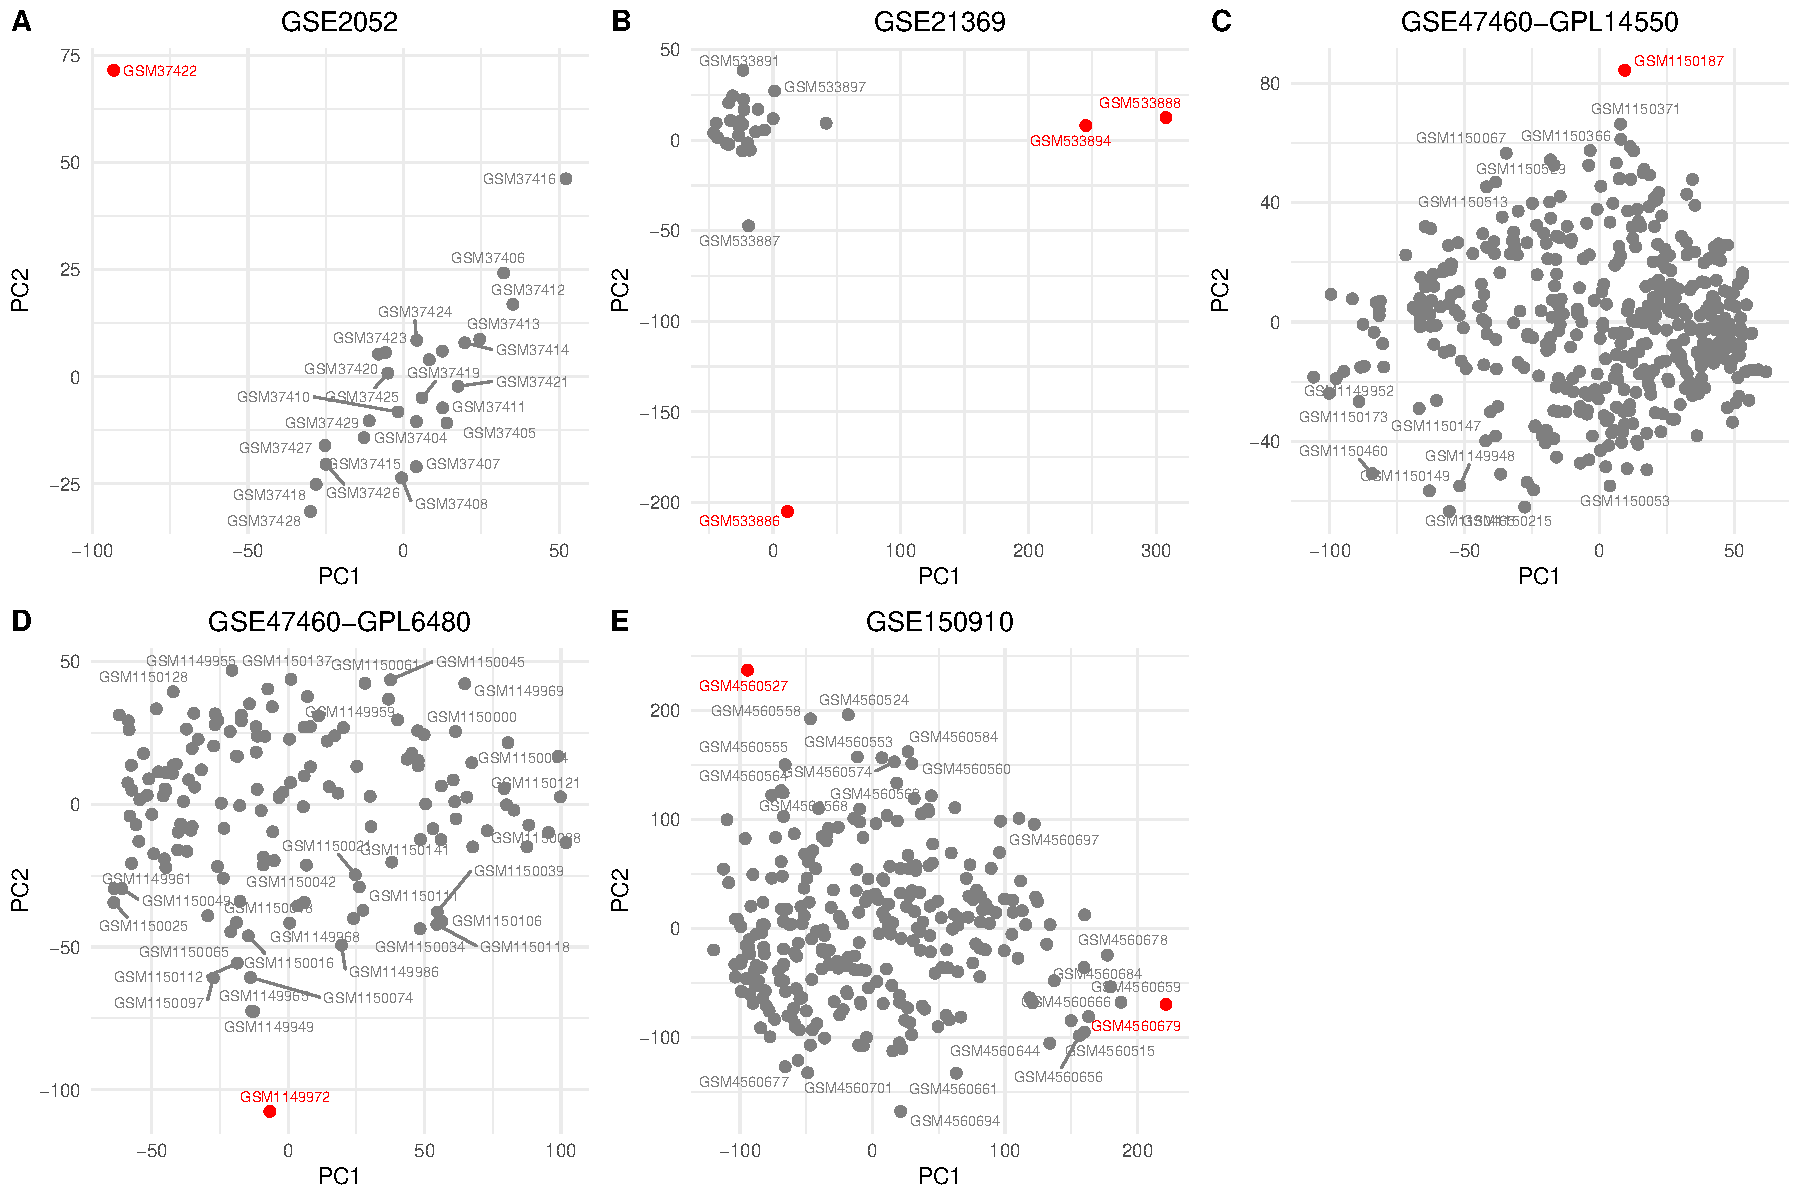
\includegraphics[width=0.9\linewidth,]{./Figures/SysReview/FigE1_outliers} 

}

\caption[Outlier detection]{\textbf{Sample outlier detection.} Principal component analysis (PCA) of author-normalized expression matrices to identify data outliers (defined as being 3 standard deviations away from the mean of principal component 1 or 2).}\label{fig:outlierPCA}
\end{figure}

\hypertarget{data}{%
\subsection{Data integration and analysis}\label{data}}

The Multivariate INTegrative (MINT) method (`mixOmics' v6.22.0) is based on partial least squares (PLS) regression. In PLS discriminant analysis (PLS-DA), latent components are constructed from linear combinations of the data matrix X variables and Y outcome to maximize covariance, and each variable is assigned a weight coefficient to indicate its importance in defining the component. PLS can also be extended to integrate data across studies (multi-group PLS), by defining global components to project samples from different studies into a common space. The MINT algorithm combines these two approaches and applies a least absolute shrinkage and selection operator (lasso) penalization for variable selection resulting in simultaneous batch correction and classification. MINT classification models are also able to handle missing data via nonlinear iterative partial least squares (NIPALS) modelling {[}\protect\hyperlink{ref-wold_nonlinear_1973}{127}{]}, so they may be applied despite missing probes or reads in the sequencing method of choice.

Datasets were integrated via shared genes and projected into a common latent space via lasso-penalized multi-group PLS (Figure \ref{fig:integration}), which identifies a small subset of variables that can discriminate classes across studies. Tuning of the lasso penalty parameter was performed via leave-one-group-out cross validation, where the optimal model was selected based on the lowest balanced error rate (BER; the average error rate in each class) with a minimum of 50 features to identify biologically important genes (Figure \ref{fig:tuningMINT}). Final model performance was then assessed using the mixOmics `perf' function against the 8 left-out test datasets, and 95\% confidence intervals obtained using the bootstrap method (Table \ref{tab:modelPerf}). Sex-specific models were also generated (Table \ref{tab:sexModel})

Pathway analyses were limited for some of our models given their relatively small number of features (e.g.~55 genes for IPF vs Control). To address this, we used the R package `bcp' (version 4.0.3) to determine models with an ``expanded'' number of features. Briefly, data from the tuning grids was analyzed to identify changepoints (i.e.~points at which the BER was likely to change). We selected the most amount of features at which the BER remained stable before increasing, as this would provide us with a high number of features without sacrificing model performance (Figure \ref{fig:bayes}). To ensure that the expanded models recapitulated the performance of the original model, we applied them to the test sets to confirm their ability to discriminate between classes (data not shown).
Gene lists from expanded models were then analyzed via overrepresentation analysis using the `cashoes/sear' package (\url{https://github.com/cashoes/sear}) (Table E8).
Custom cell pathway annotations were used for Table E9 based upon single-cell RNA-seq data from (16--19).



\begin{figure}

{\centering 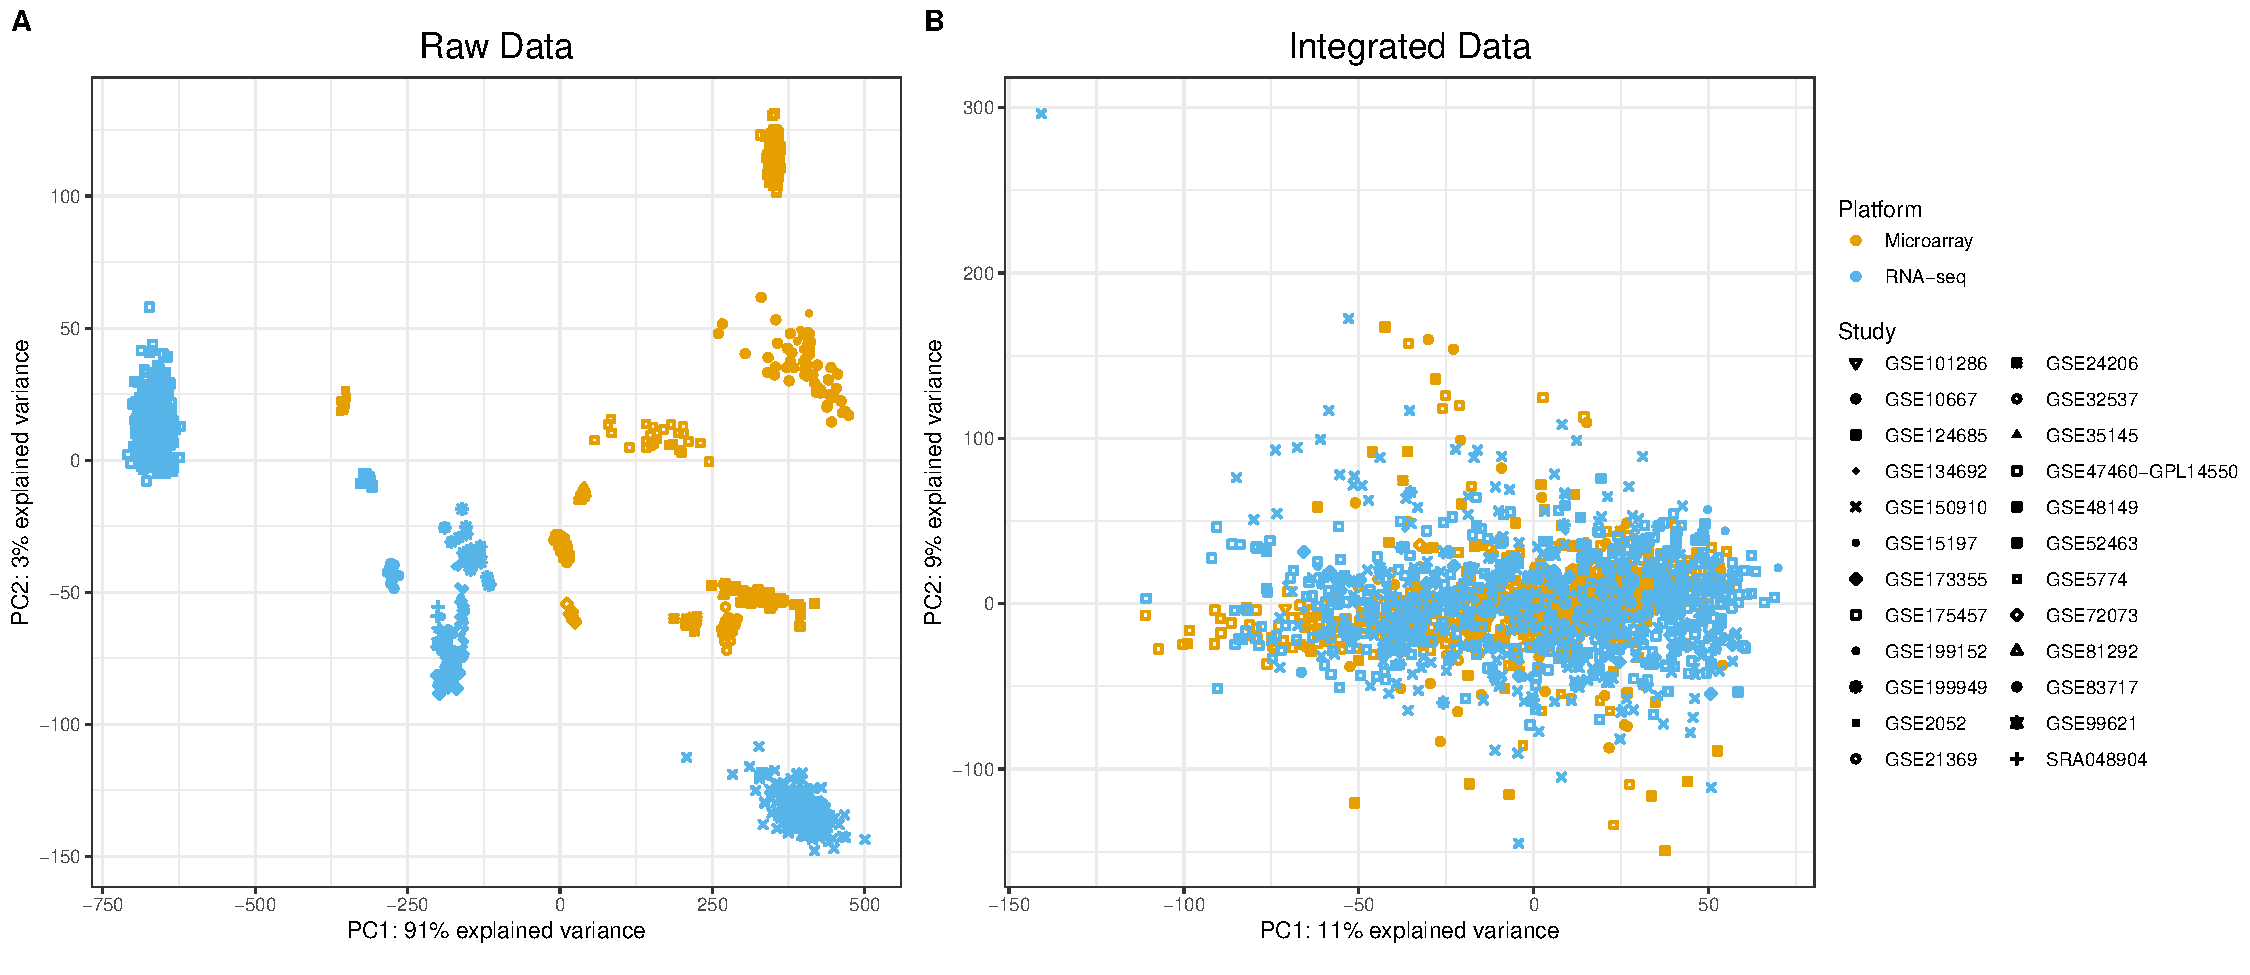
\includegraphics[width=1\linewidth,]{./Figures/SysReview/Figure2_PCA} 

}

\caption[MINT integration]{\textbf{Principal component analysis (PCA) of lung transcriptomics data prior to and after MINT integration.} Author-normalized datasets were subsetted with genes shared in \textgreater80\% of datasets (A) and integrated using MINT. MINT-integrated samples projected into a common latent space via multi-group PCA are shown in (B).}\label{fig:integration}
\end{figure}



\begin{figure}

{\centering 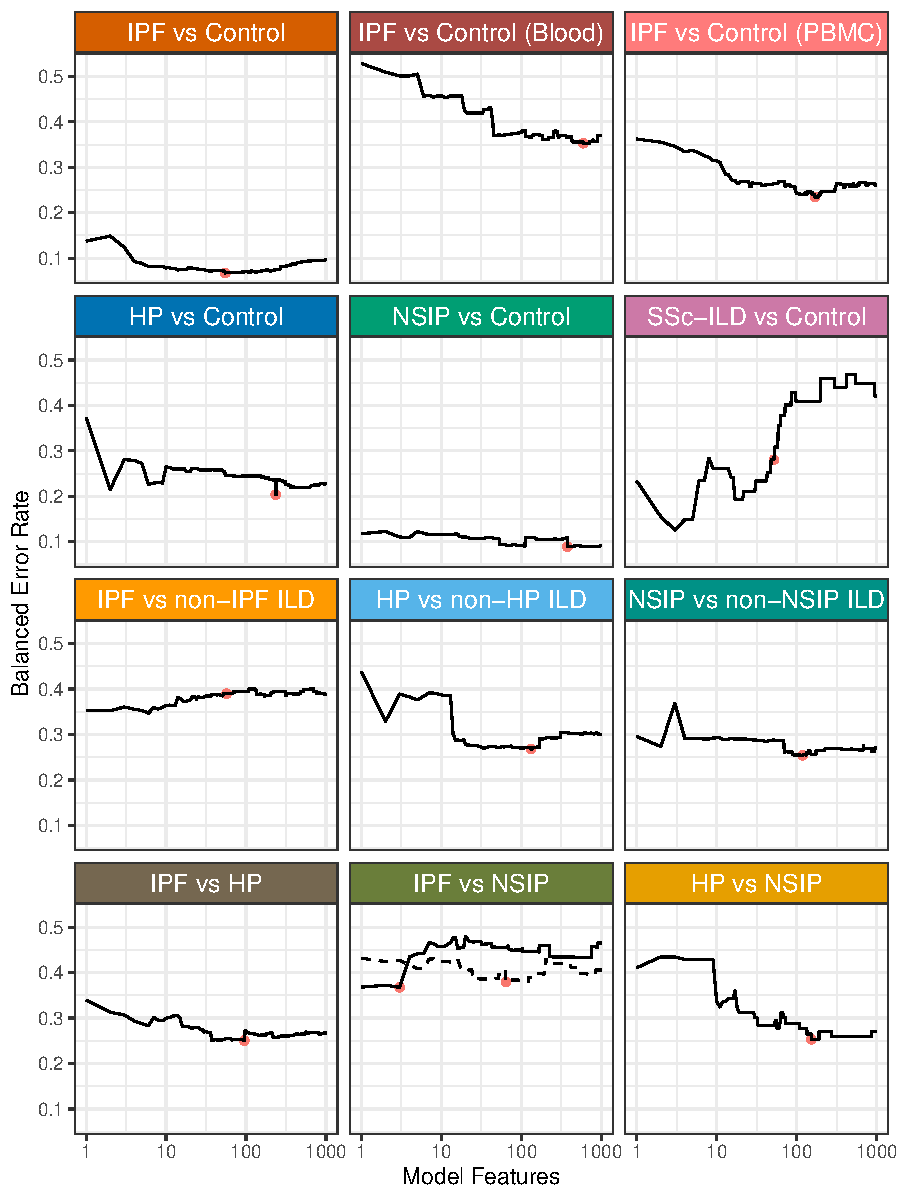
\includegraphics[width=1\linewidth,]{./Figures/SysReview/FigE2_tuning} 

}

\caption[Model tuning]{\textbf{Feature selection for MINT classification models.} Tuning grids to determine the optimal number of features (indicated by red point) for each model based on the lowest balanced error rate. All models were selected based on the lowest BER with a minimum of 50 features. For each model, one PLS component (solid line) was sufficient to separate classes with the exception of IPF vs NSIP, which required a second PLS component (dotted line).}\label{fig:tuningMINT}
\end{figure}



\begin{figure}

{\centering 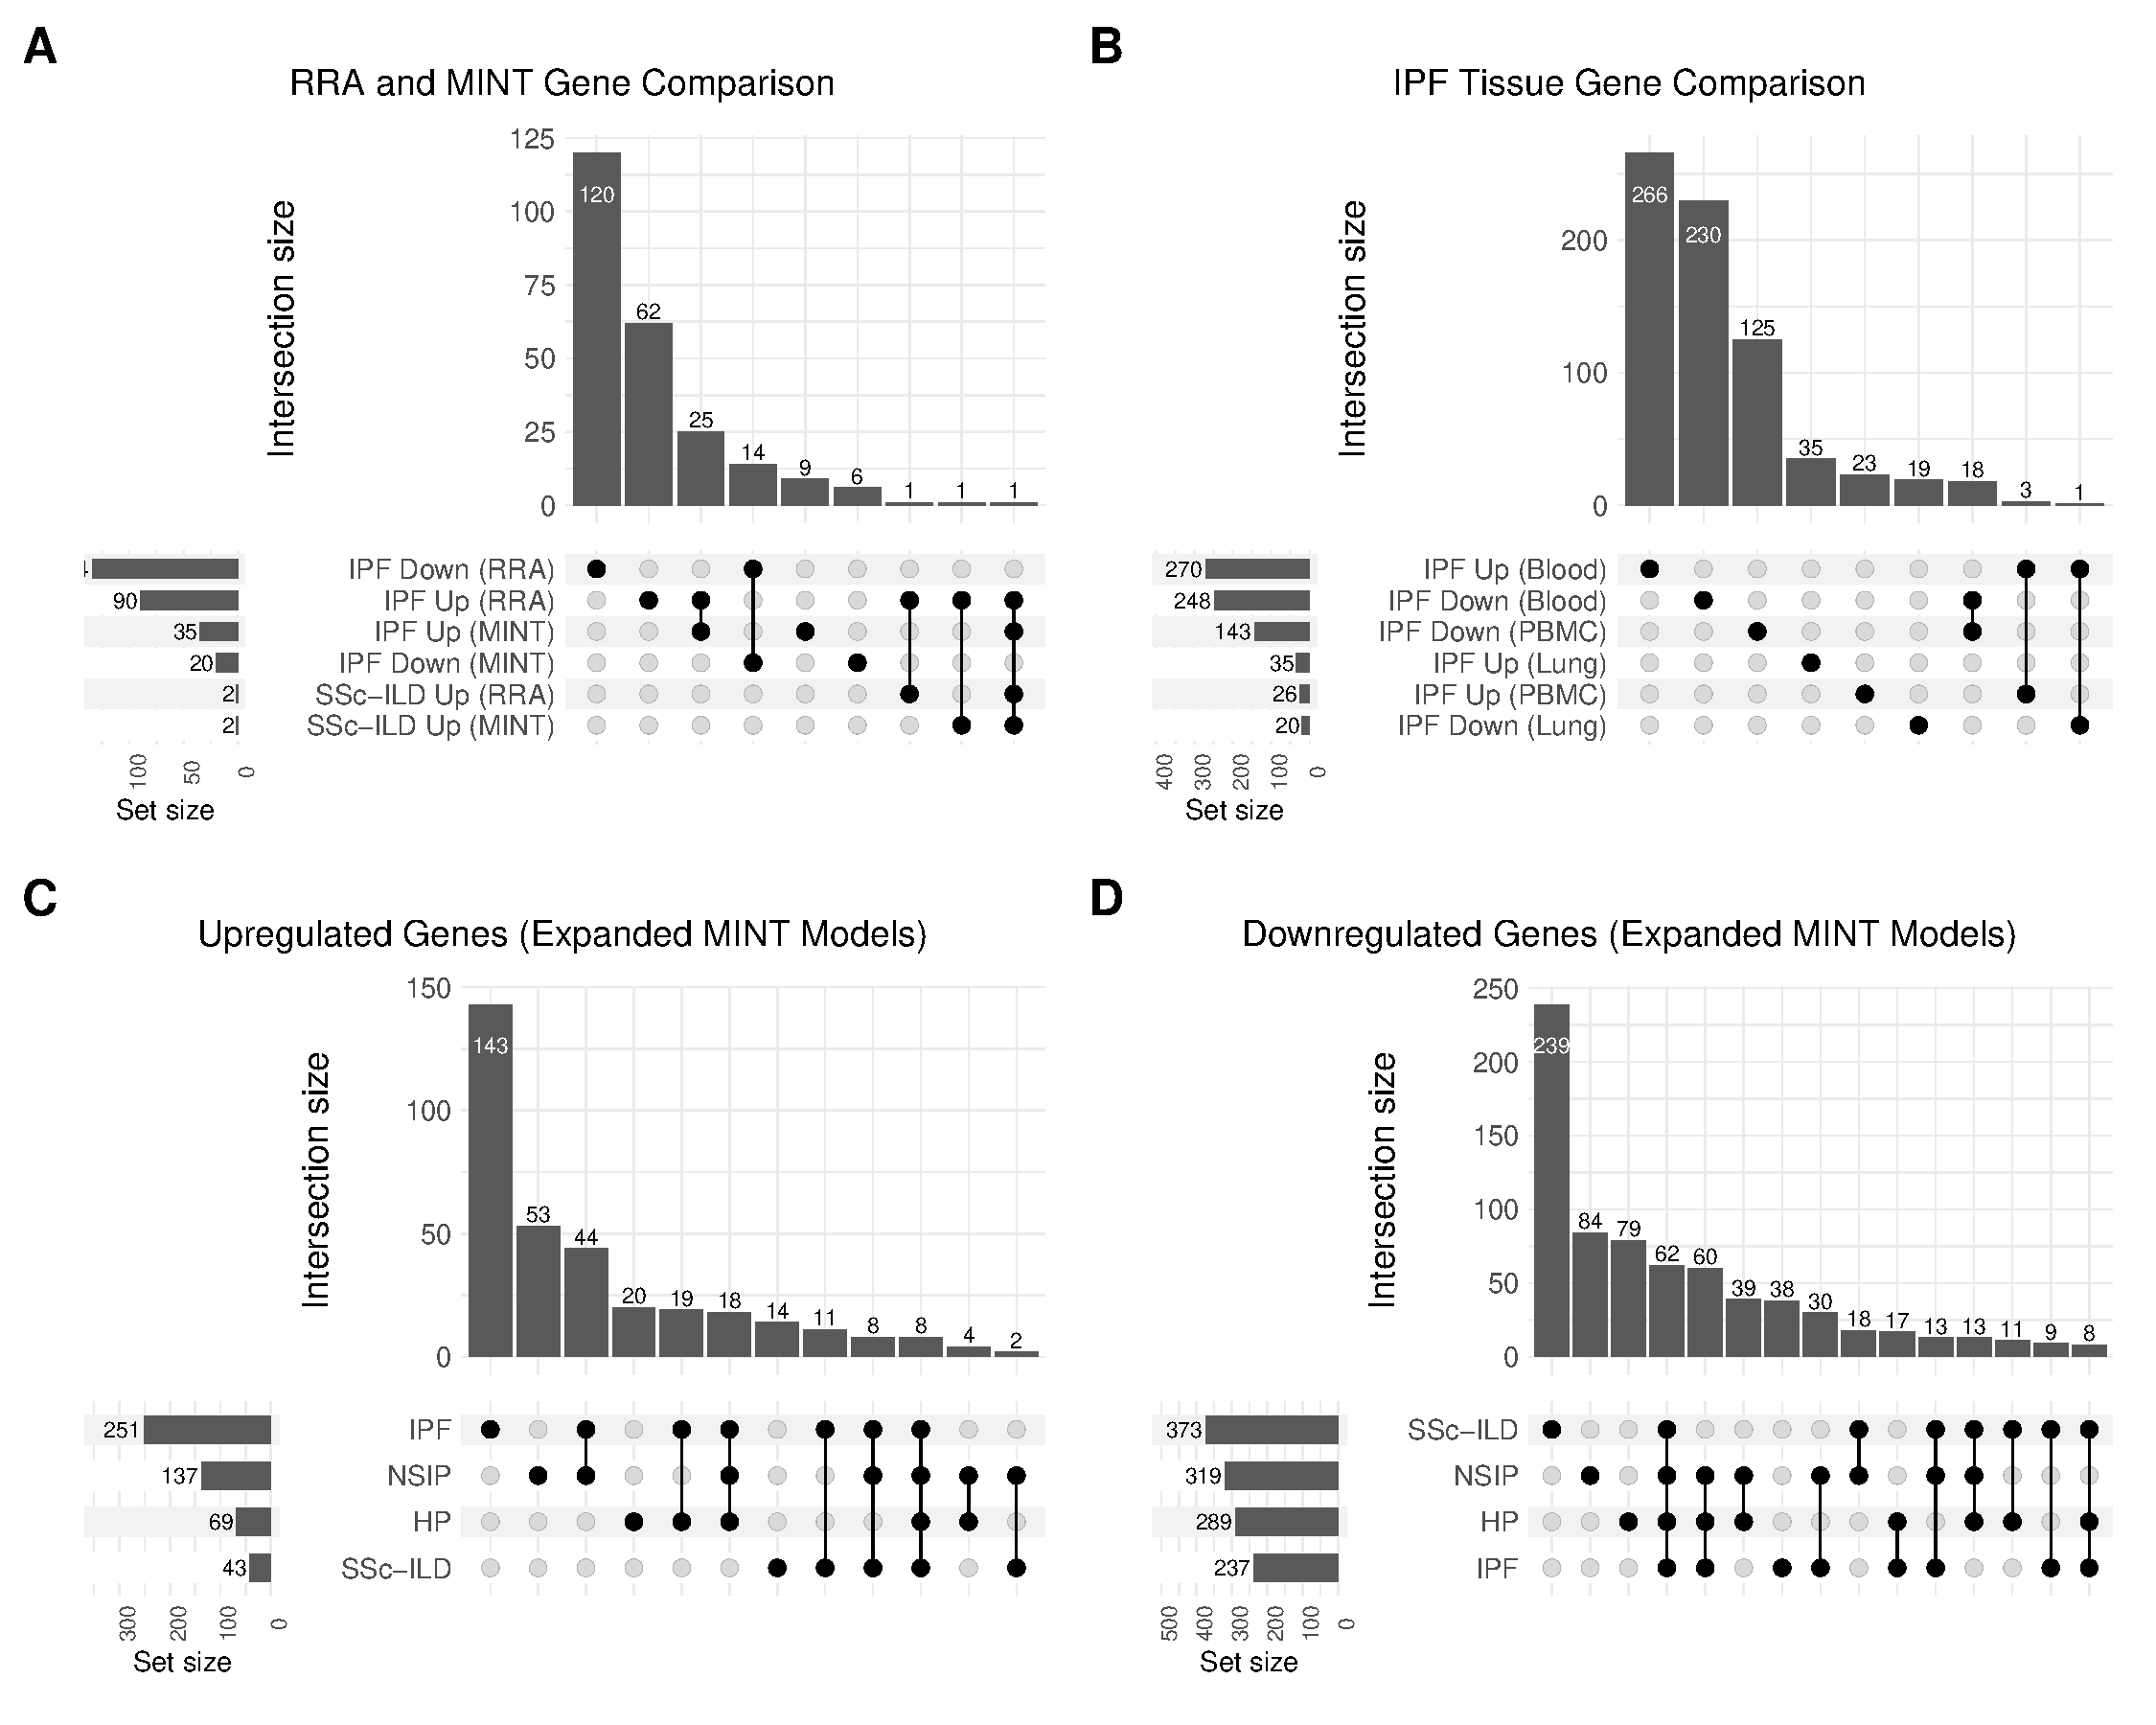
\includegraphics[width=1\linewidth,]{./Figures/SysReview/FigE3_upset} 

}

\caption[Upset plot of models]{\textbf{Upset plots of ILD vs. Control gene signatures generated by MINT.} A) Comparison of the robust rank aggregation (RRA) generated up- and down-regulated genes with MINT gene signatures. Common upregulated genes include \textit{COMP}, \textit{DIO2}, \textit{FHL2}, \textit{COL17A1}, and \textit{MMP7}, and common downregulated genes include \textit{CA4}, \textit{CRTAC1}, \textit{FAM167A}, \textit{FZD5}, \textit{MYRF}, and \textit{PLLP}. For RRA, only IPF and SSc-ILD consensus gene lists were identified. B) Comparison of gene signatures of IPF vs Control in lung, blood, and PBMC samples. C,D) Comparison of up- and down-regulated genes found in each expanded ILD subtype model again controls.}\label{fig:modelUpset}
\end{figure}



\begin{figure}

{\centering 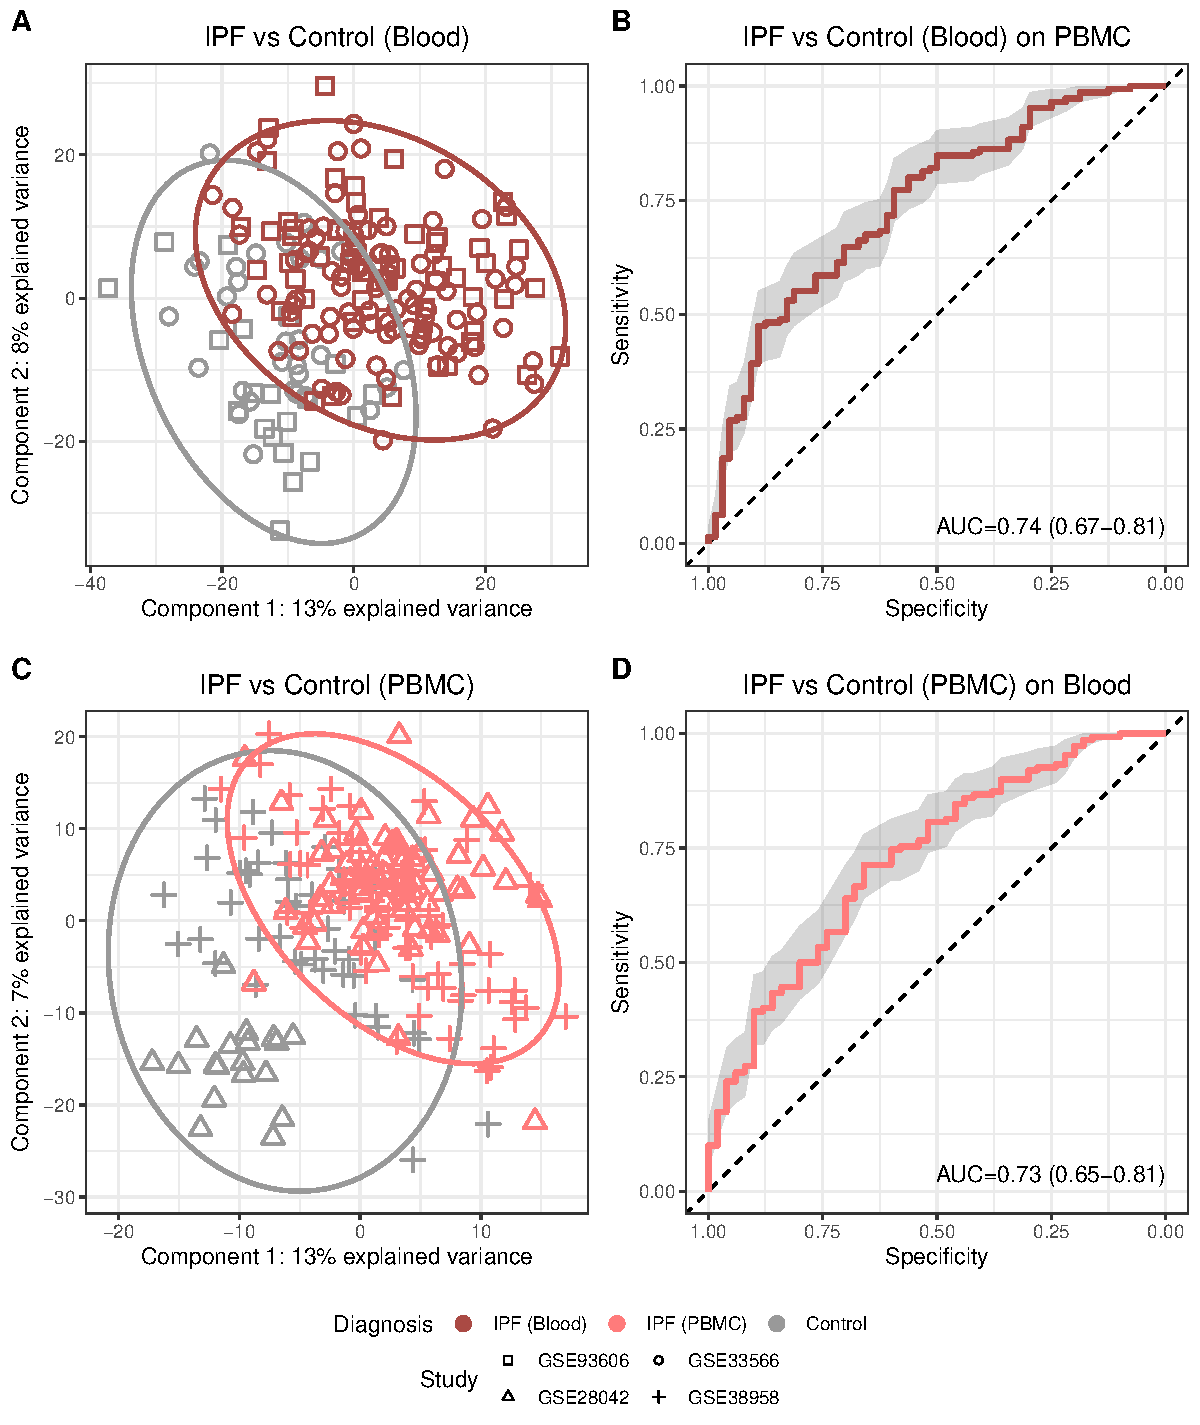
\includegraphics[width=1\linewidth,]{./Figures/SysReview/FigE4_blood} 

}

\caption[Upset plot of models]{\textbf{Classification models using IPF peripheral transcriptomics.} PLS projections of MINT classification models for IPF vs Control using whole blood (A) and PBMC (C) datasets. AUC performance of the whole blood model on the PBMC datasets (B) and PBMC model on blood datasets (D).}\label{fig:bloodmodel}
\end{figure}

\newpage

\captionsetup{width=6.5in}



\begin{table}[!h]
\centering\centering
\caption{\label{tab:modelPerf}\textbf{Summary of ILD MINT model performance on indicated test sets.} Area under receiver operating curve (AUC), balanced error rate (BER), sensitivity, and specificity were calculated using the `auroc.mint.splsda' function from mixOmics. 95\% confidence intervals (95\% C.I.) were determined via bootstrapping.}
\centering
\begin{tabu} to \linewidth {>{\raggedright\arraybackslash}p{1.75in}>{\centering\arraybackslash}p{0.5in}>{\centering\arraybackslash}p{0.7in}>{\centering\arraybackslash}p{1.25in}>{\centering\arraybackslash}p{1.25in}}
\toprule
Model & Genes & Test Sets & AUC [95\% C.I.] & BER [95\% C.I.]\\
\midrule
IPF vs Control & 55 & 8 & 0.99 [0.99-1.00] & 0.06 [0.03-0.08]\\
HP vs Control & 235 & 3 & 0.91 [0.84-0.99] & 0.13 [0.05-0.23]\\
NSIP vs Control & 378 & 4 & 0.94 [0.88-0.99] & 0.18 [0.08-0.28]\\
SSc-ILD vs Control & 52 & 1 & 0.98 [0.93-1.00] & 0.11 [0.00-0.25]\\
IPF vs nonIPF & 57 & 6 & 0.71 [0.63-0.79] & 0.35 [0.28-0.43]\\
HP vs nonHP & 132 & 2 & 0.76 [0.63-0.89] & 0.30 [0.18-0.44]\\
NSIP vs nonNSIP & 174 & 4 & 0.60 [0.49-0.72] & 0.46 [0.34-0.58]\\
IPF vs HP & 95 & 3 & 0.76 [0.64-0.87] & 0.28 [0.19-0.39]\\
IPF vs NSIP & 67 & 4 & 0.76 [0.64-0.88] & 0.32 [0.21-0.45]\\
HP vs NSIP & 153 & 2 & 0.74 [0.51-0.96] & 0.37 [0.16-0.60]\\
IPF vs Control (Blood) & 518 & 2* & 0.74 [0.67-0.81] & 0.34 [0.28-0.42]\\
IPF vs Control (PBMC) & 169 & 2** & 0.73 [0.65-0.81] & 0.33 [0.26-0.42]\\
\bottomrule
\multicolumn{5}{l}{\rule{0pt}{1em}* Performance on PBMC datasets}\\
\multicolumn{5}{l}{\rule{0pt}{1em}** Performance on whole blood datasets}\\
\end{tabu}
\end{table}



\begin{table}[!h]
\centering\centering
\caption{\label{tab:sexModel}\textbf{Summary of ILD sex-specific model performance on indicated test sets.} Area under receiver operating curve (AUC), balanced error rate (BER), sensitivity, and specificity were calculated using the `auroc.mint.splsda' function from mixOmics. 95\% confidence intervals (95\% C.I.) were determined via bootstrapping.}
\centering
\begin{tabu} to \linewidth {>{\raggedright}X>{\centering}X>{\centering}X>{\centering}X}
\toprule
Model & Test Datasets & AUC & BER\\
\midrule
IPFmale & Male & 0.98 [0.97-1.00] & 0.08 [0.05-0.13]\\
IPFmale & Female & 0.94 [0.92-0.96] & 0.09 [0.06-0.11]\\
IPFfemale & Female & 0.99 [0.96-1.00] & 0.04 [0.00-0.09]\\
IPFfemale & Male & 0.93 [0.91-0.95] & 0.06 [0.04-0.07]\\
HPmale & Male & 0.96 [0.89-1.00] & 0.11 [0.02-0.20]\\
HPmale & Female & 0.90 [0.84-0.95] & 0.15 [0.10-0.21]\\
HPfemale & Female & 0.88 [0.75-1.00] & 0.20 [0.07-0.35]\\
HPfemale & Male & 0.96 [0.93-0.99] & 0.10 [0.05-0.15]\\
NSIPmale & Male & 0.98 [0.93-1.00] & 0.15 [0.06-0.24]\\
NSIPmale & Female & 0.79 [0.68-0.90] & 0.26 [0.17-0.35]\\
NSIPfemale & Female & 0.88 [0.77-1.00] & 0.15 [0.05-0.27]\\
NSIPfemale & Male & 0.89 [0.78-0.99] & 0.18 [0.08-0.29]\\
\bottomrule
\end{tabu}
\end{table}

\pagebreak

\begin{singlespace}



\begingroup\fontsize{8}{10}\selectfont

\begin{longtable}[t]{lccc}
\caption{\label{tab:ipfgenes}\textbf{Gene weights for IPF vs Control (Lung) classification model.}}\\
\toprule
EnsemblID & Gene & Weight & Expression\\
\midrule
\endfirsthead
\caption[]{\label{tab:ipfgenes}\textbf{Gene weights for IPF vs Control (Lung) classification model.} \textit{(continued)}}\\
\toprule
EnsemblID & Gene & Weight & Expression\\
\midrule
\endhead

\endfoot
\bottomrule
\endlastfoot
ENSG00000065618 & COL17A1 & 0.3298 & IPF Upregulated\\
ENSG00000137673 & MMP7 & 0.3164 & IPF Upregulated\\
ENSG00000105664 & COMP & 0.3154 & IPF Upregulated\\
ENSG00000211448 & DIO2 & 0.3072 & IPF Upregulated\\
ENSG00000166922 & SCG5 & 0.2716 & IPF Upregulated\\
\addlinespace
ENSG00000123496 & IL13RA2 & 0.2616 & IPF Upregulated\\
ENSG00000167434 & CA4 & -0.1977 & IPF Downregulated\\
ENSG00000143320 & CRABP2 & 0.1778 & IPF Upregulated\\
ENSG00000123119 & NECAB1 & -0.1655 & IPF Downregulated\\
ENSG00000171004 & HS6ST2 & 0.1651 & IPF Upregulated\\
\addlinespace
ENSG00000164932 & CTHRC1 & 0.1539 & IPF Upregulated\\
ENSG00000115756 & HPCAL1 & -0.1454 & IPF Downregulated\\
ENSG00000115641 & FHL2 & 0.1438 & IPF Upregulated\\
ENSG00000145423 & SFRP2 & 0.1363 & IPF Upregulated\\
ENSG00000158764 & ITLN2 & -0.1320 & IPF Downregulated\\
\addlinespace
ENSG00000099953 & MMP11 & 0.1263 & IPF Upregulated\\
ENSG00000124920 & MYRF & -0.1181 & IPF Downregulated\\
ENSG00000133083 & DCLK1 & 0.1167 & IPF Upregulated\\
ENSG00000137573 & SULF1 & 0.1158 & IPF Upregulated\\
ENSG00000187955 & COL14A1 & 0.1123 & IPF Upregulated\\
\addlinespace
ENSG00000102934 & PLLP & -0.1073 & IPF Downregulated\\
ENSG00000055813 & CCDC85A & -0.1050 & IPF Downregulated\\
ENSG00000135052 & GOLM1 & 0.1027 & IPF Upregulated\\
ENSG00000105339 & DENND3 & -0.1000 & IPF Downregulated\\
ENSG00000204866 & IGFL2 & 0.0987 & IPF Upregulated\\
\addlinespace
ENSG00000105227 & PRX & -0.0978 & IPF Downregulated\\
ENSG00000155066 & PROM2 & 0.0948 & IPF Upregulated\\
ENSG00000165810 & BTNL9 & -0.0936 & IPF Downregulated\\
ENSG00000128422 & KRT17 & 0.0906 & IPF Upregulated\\
ENSG00000154319 & FAM167A & -0.0893 & IPF Downregulated\\
\addlinespace
ENSG00000127329 & PTPRB & -0.0880 & IPF Downregulated\\
ENSG00000164694 & FNDC1 & 0.0879 & IPF Upregulated\\
ENSG00000204305 & AGER & -0.0803 & IPF Downregulated\\
ENSG00000198682 & PAPSS2 & -0.0803 & IPF Downregulated\\
ENSG00000170558 & CDH2 & 0.0689 & IPF Upregulated\\
\addlinespace
ENSG00000138271 & GPR87 & 0.0670 & IPF Upregulated\\
ENSG00000204291 & COL15A1 & 0.0655 & IPF Upregulated\\
ENSG00000163251 & FZD5 & -0.0632 & IPF Downregulated\\
ENSG00000184254 & ALDH1A3 & 0.0617 & IPF Upregulated\\
ENSG00000128606 & LRRC17 & 0.0558 & IPF Upregulated\\
\addlinespace
ENSG00000196611 & MMP1 & 0.0375 & IPF Upregulated\\
ENSG00000099284 & MACROH2A2 & 0.0358 & IPF Upregulated\\
ENSG00000133019 & CHRM3 & -0.0351 & IPF Downregulated\\
ENSG00000205403 & CFI & 0.0347 & IPF Upregulated\\
ENSG00000113805 & CNTN3 & 0.0319 & IPF Upregulated\\
\addlinespace
ENSG00000123500 & COL10A1 & 0.0305 & IPF Upregulated\\
ENSG00000168952 & STXBP6 & -0.0290 & IPF Downregulated\\
ENSG00000106819 & ASPN & 0.0249 & IPF Upregulated\\
ENSG00000111666 & CHPT1 & -0.0241 & IPF Downregulated\\
ENSG00000145569 & OTULINL & -0.0134 & IPF Downregulated\\
\addlinespace
ENSG00000175928 & LRRN1 & 0.0092 & IPF Upregulated\\
ENSG00000171877 & FRMD5 & 0.0083 & IPF Upregulated\\
ENSG00000109654 & TRIM2 & 0.0054 & IPF Upregulated\\
ENSG00000135643 & KCNMB4 & -0.0037 & IPF Downregulated\\
ENSG00000182463 & TSHZ2 & 0.0014 & IPF Upregulated\\*
\end{longtable}
\endgroup{}



\begingroup\fontsize{8}{10}\selectfont

\begin{longtable}[t]{lccc}
\caption{\label{tab:ipfgenesblood}\textbf{Gene weights for IPF vs Control (Blood) classification model.}}\\
\toprule
EnsemblID & Gene & Weight & Expression\\
\midrule
\endfirsthead
\caption[]{\label{tab:ipfgenesblood}\textbf{Gene weights for IPF vs Control (Blood) classification model.} \textit{(continued)}}\\
\toprule
EnsemblID & Gene & Weight & Expression\\
\midrule
\endhead

\endfoot
\bottomrule
\endlastfoot
ENSG00000113441 & LNPEP & -0.1316 & IPF Blood Downregulated\\
ENSG00000115828 & QPCT & 0.1226 & IPF Blood Upregulated\\
ENSG00000275736 & OSCAR & 0.1221 & IPF Blood Upregulated\\
ENSG00000100985 & MMP9 & 0.1160 & IPF Blood Upregulated\\
ENSG00000100504 & PYGL & 0.1156 & IPF Blood Upregulated\\
\addlinespace
ENSG00000143569 & UBAP2L & -0.1114 & IPF Blood Downregulated\\
ENSG00000159128 & IFNGR2 & 0.1020 & IPF Blood Upregulated\\
ENSG00000136026 & CKAP4 & 0.1010 & IPF Blood Upregulated\\
ENSG00000167434 & CA4 & 0.0998 & IPF Blood Upregulated\\
ENSG00000107771 & CCSER2 & -0.0995 & IPF Blood Downregulated\\
\addlinespace
ENSG00000196177 & ACADSB & -0.0978 & IPF Blood Downregulated\\
ENSG00000121316 & PLBD1 & 0.0933 & IPF Blood Upregulated\\
ENSG00000026025 & VIM & 0.0899 & IPF Blood Upregulated\\
ENSG00000162894 & FCMR & -0.0888 & IPF Blood Downregulated\\
ENSG00000008438 & PGLYRP1 & 0.0878 & IPF Blood Upregulated\\
\addlinespace
ENSG00000161010 & MRNIP & -0.0871 & IPF Blood Downregulated\\
ENSG00000196352 & CD55 & 0.0860 & IPF Blood Upregulated\\
ENSG00000134198 & TSPAN2 & 0.0840 & IPF Blood Upregulated\\
ENSG00000112182 & BACH2 & -0.0830 & IPF Blood Downregulated\\
ENSG00000005810 & MYCBP2 & -0.0826 & IPF Blood Downregulated\\
\addlinespace
ENSG00000182866 & LCK & -0.0814 & IPF Blood Downregulated\\
ENSG00000113269 & RNF130 & 0.0798 & IPF Blood Upregulated\\
ENSG00000176463 & SLCO3A1 & 0.0795 & IPF Blood Upregulated\\
ENSG00000111371 & SLC38A1 & -0.0794 & IPF Blood Downregulated\\
ENSG00000198734 & F5 & 0.0794 & IPF Blood Upregulated\\
\addlinespace
ENSG00000136810 & TXN & 0.0777 & IPF Blood Upregulated\\
ENSG00000221869 & CEBPD & 0.0774 & IPF Blood Upregulated\\
ENSG00000197208 & SLC22A4 & 0.0770 & IPF Blood Upregulated\\
ENSG00000186205 & MTARC1 & 0.0755 & IPF Blood Upregulated\\
ENSG00000197296 & FITM2 & -0.0753 & IPF Blood Downregulated\\
\addlinespace
ENSG00000173114 & LRRN3 & -0.0747 & IPF Blood Downregulated\\
ENSG00000206650 & SNORA70G & -0.0747 & IPF Blood Downregulated\\
ENSG00000142405 & NLRP12 & 0.0740 & IPF Blood Upregulated\\
ENSG00000163221 & S100A12 & 0.0729 & IPF Blood Upregulated\\
ENSG00000148180 & GSN & 0.0728 & IPF Blood Upregulated\\
\addlinespace
ENSG00000157106 & SMG1 & -0.0726 & IPF Blood Downregulated\\
ENSG00000120306 & CYSTM1 & 0.0721 & IPF Blood Upregulated\\
ENSG00000145491 & ROPN1L & 0.0720 & IPF Blood Upregulated\\
ENSG00000170525 & PFKFB3 & 0.0700 & IPF Blood Upregulated\\
ENSG00000277846 & SNORD30 & -0.0699 & IPF Blood Downregulated\\
\addlinespace
ENSG00000099204 & ABLIM1 & -0.0682 & IPF Blood Downregulated\\
ENSG00000274544 & SNORD28 & -0.0678 & IPF Blood Downregulated\\
ENSG00000106348 & IMPDH1 & 0.0677 & IPF Blood Upregulated\\
ENSG00000172216 & CEBPB & 0.0672 & IPF Blood Upregulated\\
ENSG00000012779 & ALOX5 & 0.0669 & IPF Blood Upregulated\\
\addlinespace
ENSG00000140743 & CDR2 & -0.0663 & IPF Blood Downregulated\\
ENSG00000115507 & OTX1 & 0.0661 & IPF Blood Upregulated\\
ENSG00000151150 & ANK3 & -0.0656 & IPF Blood Downregulated\\
ENSG00000116717 & GADD45A & 0.0651 & IPF Blood Upregulated\\
ENSG00000146021 & KLHL3 & -0.0644 & IPF Blood Downregulated\\
\addlinespace
ENSG00000276776 & TC2N & -0.0637 & IPF Blood Downregulated\\
ENSG00000118508 & RAB32 & 0.0637 & IPF Blood Upregulated\\
ENSG00000183762 & KREMEN1 & 0.0632 & IPF Blood Upregulated\\
ENSG00000182568 & SATB1 & -0.0629 & IPF Blood Downregulated\\
ENSG00000127946 & HIP1 & 0.0628 & IPF Blood Upregulated\\
\addlinespace
ENSG00000160703 & NLRX1 & 0.0625 & IPF Blood Upregulated\\
ENSG00000135636 & DYSF & 0.0613 & IPF Blood Upregulated\\
ENSG00000136709 & WDR33 & -0.0603 & IPF Blood Downregulated\\
ENSG00000135334 & AKIRIN2 & 0.0595 & IPF Blood Upregulated\\
ENSG00000151623 & NR3C2 & -0.0592 & IPF Blood Downregulated\\
\addlinespace
ENSG00000139132 & FGD4 & 0.0591 & IPF Blood Upregulated\\
ENSG00000162735 & PEX19 & -0.0584 & IPF Blood Downregulated\\
ENSG00000204577 & LILRB3 & 0.0578 & IPF Blood Upregulated\\
ENSG00000274914 & LILRA5 & 0.0576 & IPF Blood Upregulated\\
ENSG00000166326 & TRIM44 & -0.0572 & IPF Blood Downregulated\\
\addlinespace
ENSG00000158825 & CDA & 0.0572 & IPF Blood Upregulated\\
ENSG00000186431 & FCAR & 0.0568 & IPF Blood Upregulated\\
ENSG00000113263 & ITK & -0.0566 & IPF Blood Downregulated\\
ENSG00000175806 & MSRA & 0.0566 & IPF Blood Upregulated\\
ENSG00000144134 & RABL2A & -0.0562 & IPF Blood Downregulated\\
\addlinespace
ENSG00000130714 & POMT1 & -0.0562 & IPF Blood Downregulated\\
ENSG00000090861 & AARS1 & -0.0553 & IPF Blood Downregulated\\
ENSG00000158711 & ELK4 & -0.0552 & IPF Blood Downregulated\\
ENSG00000151651 & ADAM8 & 0.0551 & IPF Blood Upregulated\\
ENSG00000110931 & CAMKK2 & 0.0549 & IPF Blood Upregulated\\
\addlinespace
ENSG00000109743 & BST1 & 0.0547 & IPF Blood Upregulated\\
ENSG00000154814 & OXNAD1 & -0.0547 & IPF Blood Downregulated\\
ENSG00000229314 & ORM1 & 0.0545 & IPF Blood Upregulated\\
ENSG00000139178 & C1RL & 0.0544 & IPF Blood Upregulated\\
ENSG00000011295 & TTC19 & -0.0544 & IPF Blood Downregulated\\
\addlinespace
ENSG00000070540 & WIPI1 & 0.0543 & IPF Blood Upregulated\\
ENSG00000162231 & NXF1 & -0.0536 & IPF Blood Downregulated\\
ENSG00000172575 & RASGRP1 & -0.0535 & IPF Blood Downregulated\\
ENSG00000238597 & SNORD4B & -0.0535 & IPF Blood Downregulated\\
ENSG00000261984 & TAS2R14 & -0.0533 & IPF Blood Downregulated\\
\addlinespace
ENSG00000159339 & PADI4 & 0.0532 & IPF Blood Upregulated\\
ENSG00000079974 & RABL2B & -0.0522 & IPF Blood Downregulated\\
ENSG00000138433 & CIR1 & 0.0520 & IPF Blood Upregulated\\
ENSG00000162444 & RBP7 & 0.0518 & IPF Blood Upregulated\\
ENSG00000111261 & MANSC1 & 0.0514 & IPF Blood Upregulated\\
\addlinespace
ENSG00000115129 & TP53I3 & 0.0510 & IPF Blood Upregulated\\
ENSG00000104870 & FCGRT & 0.0509 & IPF Blood Upregulated\\
ENSG00000118520 & ARG1 & 0.0507 & IPF Blood Upregulated\\
ENSG00000166527 & CLEC4D & 0.0505 & IPF Blood Upregulated\\
ENSG00000198821 & CD247 & -0.0504 & IPF Blood Downregulated\\
\addlinespace
ENSG00000204936 & CD177 & 0.0502 & IPF Blood Upregulated\\
ENSG00000103490 & PYCARD & 0.0501 & IPF Blood Upregulated\\
ENSG00000184613 & NELL2 & -0.0493 & IPF Blood Downregulated\\
ENSG00000074966 & TXK & -0.0490 & IPF Blood Downregulated\\
ENSG00000169635 & HIC2 & -0.0489 & IPF Blood Downregulated\\
\addlinespace
ENSG00000138772 & ANXA3 & 0.0488 & IPF Blood Upregulated\\
ENSG00000138678 & GPAT3 & 0.0487 & IPF Blood Upregulated\\
ENSG00000074696 & HACD3 & -0.0482 & IPF Blood Downregulated\\
ENSG00000112053 & SLC26A8 & 0.0477 & IPF Blood Upregulated\\
ENSG00000148926 & ADM & 0.0476 & IPF Blood Upregulated\\
\addlinespace
ENSG00000101474 & APMAP & 0.0476 & IPF Blood Upregulated\\
ENSG00000243943 & ZNF512 & -0.0473 & IPF Blood Downregulated\\
ENSG00000166881 & NEMP1 & -0.0472 & IPF Blood Downregulated\\
ENSG00000146828 & SLC12A9 & 0.0471 & IPF Blood Upregulated\\
ENSG00000133256 & PDE6B & -0.0471 & IPF Blood Downregulated\\
\addlinespace
ENSG00000206760 & SNORA6 & -0.0462 & IPF Blood Downregulated\\
ENSG00000132953 & XPO4 & -0.0459 & IPF Blood Downregulated\\
ENSG00000136717 & BIN1 & -0.0457 & IPF Blood Downregulated\\
ENSG00000178814 & OPLAH & 0.0456 & IPF Blood Upregulated\\
ENSG00000128739 & SNRPN & -0.0455 & IPF Blood Downregulated\\
\addlinespace
ENSG00000127152 & BCL11B & -0.0454 & IPF Blood Downregulated\\
ENSG00000181722 & ZBTB20 & -0.0454 & IPF Blood Downregulated\\
ENSG00000171861 & MRM3 & -0.0453 & IPF Blood Downregulated\\
ENSG00000163754 & GYG1 & 0.0452 & IPF Blood Upregulated\\
ENSG00000120129 & DUSP1 & 0.0451 & IPF Blood Upregulated\\
\addlinespace
ENSG00000203710 & CR1 & 0.0450 & IPF Blood Upregulated\\
ENSG00000155657 & TTN & -0.0448 & IPF Blood Downregulated\\
ENSG00000173614 & NMNAT1 & 0.0448 & IPF Blood Upregulated\\
ENSG00000148841 & ITPRIP & 0.0447 & IPF Blood Upregulated\\
ENSG00000169914 & OTUD3 & -0.0446 & IPF Blood Downregulated\\
\addlinespace
ENSG00000129351 & ILF3 & -0.0445 & IPF Blood Downregulated\\
ENSG00000084090 & STARD7 & -0.0443 & IPF Blood Downregulated\\
ENSG00000262612 & TAS2R43 & -0.0442 & IPF Blood Downregulated\\
ENSG00000136111 & TBC1D4 & -0.0438 & IPF Blood Downregulated\\
ENSG00000118922 & KLF12 & -0.0437 & IPF Blood Downregulated\\
\addlinespace
ENSG00000127334 & DYRK2 & -0.0436 & IPF Blood Downregulated\\
ENSG00000167874 & TMEM88 & 0.0436 & IPF Blood Upregulated\\
ENSG00000167664 & TMIGD2 & -0.0434 & IPF Blood Downregulated\\
ENSG00000197006 & METTL9 & 0.0427 & IPF Blood Upregulated\\
ENSG00000176225 & RTTN & -0.0425 & IPF Blood Downregulated\\
\addlinespace
ENSG00000181274 & FRAT2 & 0.0424 & IPF Blood Upregulated\\
ENSG00000171456 & ASXL1 & -0.0424 & IPF Blood Downregulated\\
ENSG00000275043 & SNORD25 & -0.0423 & IPF Blood Downregulated\\
ENSG00000135905 & DOCK10 & -0.0422 & IPF Blood Downregulated\\
ENSG00000182022 & CHST15 & 0.0421 & IPF Blood Upregulated\\
\addlinespace
ENSG00000142409 & ZNF787 & 0.0421 & IPF Blood Upregulated\\
ENSG00000101493 & ZNF516 & 0.0419 & IPF Blood Upregulated\\
ENSG00000189077 & TMEM120A & 0.0418 & IPF Blood Upregulated\\
ENSG00000164104 & HMGB2 & 0.0417 & IPF Blood Upregulated\\
ENSG00000154310 & TNIK & -0.0413 & IPF Blood Downregulated\\
\addlinespace
ENSG00000177191 & B3GNT8 & 0.0411 & IPF Blood Upregulated\\
ENSG00000111424 & VDR & 0.0411 & IPF Blood Upregulated\\
ENSG00000080561 & MID2 & -0.0407 & IPF Blood Downregulated\\
ENSG00000111885 & MAN1A1 & 0.0406 & IPF Blood Upregulated\\
ENSG00000116260 & QSOX1 & 0.0404 & IPF Blood Upregulated\\
\addlinespace
ENSG00000105501 & SIGLEC5 & 0.0399 & IPF Blood Upregulated\\
ENSG00000160883 & HK3 & 0.0396 & IPF Blood Upregulated\\
ENSG00000130844 & ZNF331 & -0.0396 & IPF Blood Downregulated\\
ENSG00000130684 & ZNF337 & -0.0391 & IPF Blood Downregulated\\
ENSG00000196663 & TECPR2 & 0.0390 & IPF Blood Upregulated\\
\addlinespace
ENSG00000109016 & DHRS7B & 0.0390 & IPF Blood Upregulated\\
ENSG00000197063 & MAFG & 0.0389 & IPF Blood Upregulated\\
ENSG00000168297 & PXK & 0.0388 & IPF Blood Upregulated\\
ENSG00000117174 & ZNHIT6 & -0.0385 & IPF Blood Downregulated\\
ENSG00000183696 & UPP1 & 0.0385 & IPF Blood Upregulated\\
\addlinespace
ENSG00000166523 & CLEC4E & 0.0380 & IPF Blood Upregulated\\
ENSG00000162777 & DENND2D & -0.0377 & IPF Blood Downregulated\\
ENSG00000112159 & MDN1 & -0.0371 & IPF Blood Downregulated\\
ENSG00000228502 & EEF1A1P11 & -0.0369 & IPF Blood Downregulated\\
ENSG00000118058 & KMT2A & -0.0368 & IPF Blood Downregulated\\
\addlinespace
ENSG00000069667 & RORA & -0.0366 & IPF Blood Downregulated\\
ENSG00000277377 & SERPINA1 & 0.0365 & IPF Blood Upregulated\\
ENSG00000113916 & BCL6 & 0.0364 & IPF Blood Upregulated\\
ENSG00000157551 & KCNJ15 & 0.0361 & IPF Blood Upregulated\\
ENSG00000170876 & TMEM43 & 0.0360 & IPF Blood Upregulated\\
\addlinespace
ENSG00000141480 & ARRB2 & 0.0358 & IPF Blood Upregulated\\
ENSG00000178562 & CD28 & -0.0357 & IPF Blood Downregulated\\
ENSG00000116991 & SIPA1L2 & 0.0355 & IPF Blood Upregulated\\
ENSG00000215252 & GOLGA8B & -0.0354 & IPF Blood Downregulated\\
ENSG00000051620 & HEBP2 & 0.0354 & IPF Blood Upregulated\\
\addlinespace
ENSG00000033327 & GAB2 & 0.0352 & IPF Blood Upregulated\\
ENSG00000155561 & NUP205 & -0.0349 & IPF Blood Downregulated\\
ENSG00000050426 & LETMD1 & -0.0345 & IPF Blood Downregulated\\
ENSG00000125245 & GPR18 & -0.0344 & IPF Blood Downregulated\\
ENSG00000133561 & GIMAP6 & -0.0342 & IPF Blood Downregulated\\
\addlinespace
ENSG00000275342 & PRAG1 & -0.0342 & IPF Blood Downregulated\\
ENSG00000156239 & N6AMT1 & -0.0340 & IPF Blood Downregulated\\
ENSG00000007237 & GAS7 & 0.0337 & IPF Blood Upregulated\\
ENSG00000152795 & HNRNPDL & -0.0336 & IPF Blood Downregulated\\
ENSG00000134987 & WDR36 & -0.0335 & IPF Blood Downregulated\\
\addlinespace
ENSG00000197321 & SVIL & 0.0329 & IPF Blood Upregulated\\
ENSG00000168758 & SEMA4C & -0.0328 & IPF Blood Downregulated\\
ENSG00000111052 & LIN7A & 0.0328 & IPF Blood Upregulated\\
ENSG00000123810 & B9D2 & 0.0327 & IPF Blood Upregulated\\
ENSG00000072401 & UBE2D1 & 0.0327 & IPF Blood Upregulated\\
\addlinespace
ENSG00000168685 & IL7R & -0.0327 & IPF Blood Downregulated\\
ENSG00000184677 & ZBTB40 & -0.0327 & IPF Blood Downregulated\\
ENSG00000164023 & SGMS2 & 0.0325 & IPF Blood Upregulated\\
ENSG00000122642 & FKBP9 & 0.0325 & IPF Blood Upregulated\\
ENSG00000189079 & ARID2 & -0.0324 & IPF Blood Downregulated\\
\addlinespace
ENSG00000167995 & BEST1 & 0.0323 & IPF Blood Upregulated\\
ENSG00000035862 & TIMP2 & 0.0322 & IPF Blood Upregulated\\
ENSG00000165801 & ARHGEF40 & 0.0322 & IPF Blood Upregulated\\
ENSG00000152642 & GPD1L & -0.0321 & IPF Blood Downregulated\\
ENSG00000176845 & METRNL & 0.0321 & IPF Blood Upregulated\\
\addlinespace
ENSG00000170345 & FOS & 0.0321 & IPF Blood Upregulated\\
ENSG00000147274 & RBMX & -0.0316 & IPF Blood Downregulated\\
ENSG00000148824 & MTG1 & -0.0313 & IPF Blood Downregulated\\
ENSG00000196411 & EPHB4 & 0.0307 & IPF Blood Upregulated\\
ENSG00000143409 & MINDY1 & 0.0305 & IPF Blood Upregulated\\
\addlinespace
ENSG00000196405 & EVL & -0.0305 & IPF Blood Downregulated\\
ENSG00000027075 & PRKCH & -0.0300 & IPF Blood Downregulated\\
ENSG00000188315 & C3orf62 & 0.0299 & IPF Blood Upregulated\\
ENSG00000122224 & LY9 & -0.0299 & IPF Blood Downregulated\\
ENSG00000121310 & ECHDC2 & -0.0299 & IPF Blood Downregulated\\
\addlinespace
ENSG00000115590 & IL1R2 & 0.0297 & IPF Blood Upregulated\\
ENSG00000164713 & BRI3 & 0.0296 & IPF Blood Upregulated\\
ENSG00000180316 & PNPLA1 & 0.0296 & IPF Blood Upregulated\\
ENSG00000025039 & RRAGD & 0.0295 & IPF Blood Upregulated\\
ENSG00000175676 & GOLGA8DP & -0.0293 & IPF Blood Downregulated\\
\addlinespace
ENSG00000102580 & DNAJC3 & 0.0293 & IPF Blood Upregulated\\
ENSG00000100218 & RSPH14 & 0.0293 & IPF Blood Upregulated\\
ENSG00000275996 & SNORD27 & -0.0292 & IPF Blood Downregulated\\
ENSG00000152495 & CAMK4 & -0.0289 & IPF Blood Downregulated\\
ENSG00000174197 & MGA & -0.0288 & IPF Blood Downregulated\\
\addlinespace
ENSG00000021355 & SERPINB1 & 0.0286 & IPF Blood Upregulated\\
ENSG00000171488 & LRRC8C & -0.0283 & IPF Blood Downregulated\\
ENSG00000134852 & CLOCK & -0.0280 & IPF Blood Downregulated\\
ENSG00000139746 & RBM26 & -0.0278 & IPF Blood Downregulated\\
ENSG00000100228 & RAB36 & 0.0275 & IPF Blood Upregulated\\
\addlinespace
ENSG00000161381 & PLXDC1 & -0.0271 & IPF Blood Downregulated\\
ENSG00000276788 & SNORD26 & -0.0271 & IPF Blood Downregulated\\
ENSG00000161040 & FBXL13 & 0.0270 & IPF Blood Upregulated\\
ENSG00000197956 & S100A6 & 0.0268 & IPF Blood Upregulated\\
ENSG00000215788 & TNFRSF25 & -0.0265 & IPF Blood Downregulated\\
\addlinespace
ENSG00000114423 & CBLB & -0.0262 & IPF Blood Downregulated\\
ENSG00000143167 & GPA33 & -0.0262 & IPF Blood Downregulated\\
ENSG00000162702 & ZNF281 & 0.0260 & IPF Blood Upregulated\\
ENSG00000099622 & CIRBP & -0.0259 & IPF Blood Downregulated\\
ENSG00000215196 & BASP1-AS1 & 0.0259 & IPF Blood Upregulated\\
\addlinespace
ENSG00000100316 & RPL3 & -0.0258 & IPF Blood Downregulated\\
ENSG00000177156 & TALDO1 & 0.0257 & IPF Blood Upregulated\\
ENSG00000197603 & CPLANE1 & -0.0256 & IPF Blood Downregulated\\
ENSG00000188786 & MTF1 & 0.0256 & IPF Blood Upregulated\\
ENSG00000107679 & PLEKHA1 & -0.0256 & IPF Blood Downregulated\\
\addlinespace
ENSG00000145982 & FARS2 & -0.0255 & IPF Blood Downregulated\\
ENSG00000181827 & RFX7 & -0.0255 & IPF Blood Downregulated\\
ENSG00000179862 & CITED4 & 0.0254 & IPF Blood Upregulated\\
ENSG00000128594 & LRRC4 & 0.0254 & IPF Blood Upregulated\\
ENSG00000119977 & TCTN3 & -0.0254 & IPF Blood Downregulated\\
\addlinespace
ENSG00000134686 & PHC2 & 0.0253 & IPF Blood Upregulated\\
ENSG00000167106 & EEIG1 & -0.0250 & IPF Blood Downregulated\\
ENSG00000079277 & MKNK1 & 0.0250 & IPF Blood Upregulated\\
ENSG00000164180 & TMEM161B & -0.0250 & IPF Blood Downregulated\\
ENSG00000136444 & RSAD1 & -0.0250 & IPF Blood Downregulated\\
\addlinespace
ENSG00000021776 & AQR & -0.0248 & IPF Blood Downregulated\\
ENSG00000087903 & RFX2 & 0.0248 & IPF Blood Upregulated\\
ENSG00000154473 & BUB3 & -0.0244 & IPF Blood Downregulated\\
ENSG00000237808 & NCR3 & -0.0244 & IPF Blood Downregulated\\
ENSG00000260916 & CCPG1 & 0.0243 & IPF Blood Upregulated\\
\addlinespace
ENSG00000135678 & CPM & 0.0243 & IPF Blood Upregulated\\
ENSG00000128311 & TST & 0.0242 & IPF Blood Upregulated\\
ENSG00000154027 & AK5 & -0.0240 & IPF Blood Downregulated\\
ENSG00000189159 & JPT1 & 0.0240 & IPF Blood Upregulated\\
ENSG00000131067 & GGT7 & -0.0240 & IPF Blood Downregulated\\
\addlinespace
ENSG00000169508 & GPR183 & -0.0239 & IPF Blood Downregulated\\
ENSG00000173083 & HPSE & 0.0234 & IPF Blood Upregulated\\
ENSG00000150403 & TMCO3 & 0.0233 & IPF Blood Upregulated\\
ENSG00000091106 & NLRC4 & 0.0233 & IPF Blood Upregulated\\
ENSG00000011523 & CEP68 & -0.0230 & IPF Blood Downregulated\\
\addlinespace
ENSG00000008516 & MMP25 & 0.0229 & IPF Blood Upregulated\\
ENSG00000169896 & ITGAM & 0.0228 & IPF Blood Upregulated\\
ENSG00000164047 & CAMP & 0.0226 & IPF Blood Upregulated\\
ENSG00000145191 & EIF2B5 & -0.0226 & IPF Blood Downregulated\\
ENSG00000011422 & PLAUR & 0.0226 & IPF Blood Upregulated\\
\addlinespace
ENSG00000090316 & MAEA & 0.0225 & IPF Blood Upregulated\\
ENSG00000104731 & KLHDC4 & -0.0225 & IPF Blood Downregulated\\
ENSG00000183336 & BOLA2 & -0.0224 & IPF Blood Downregulated\\
ENSG00000085415 & SEH1L & -0.0224 & IPF Blood Downregulated\\
ENSG00000257335 & MGAM & 0.0222 & IPF Blood Upregulated\\
\addlinespace
ENSG00000013810 & TACC3 & 0.0221 & IPF Blood Upregulated\\
ENSG00000105514 & RAB3D & 0.0221 & IPF Blood Upregulated\\
ENSG00000137880 & GCHFR & -0.0220 & IPF Blood Downregulated\\
ENSG00000064763 & FAR2 & 0.0219 & IPF Blood Upregulated\\
ENSG00000163932 & PRKCD & 0.0219 & IPF Blood Upregulated\\
\addlinespace
ENSG00000284387 & MIR24-2 & 0.0219 & IPF Blood Upregulated\\
ENSG00000111796 & KLRB1 & -0.0218 & IPF Blood Downregulated\\
ENSG00000145833 & DDX46 & -0.0217 & IPF Blood Downregulated\\
ENSG00000058272 & PPP1R12A & 0.0217 & IPF Blood Upregulated\\
ENSG00000197324 & LRP10 & 0.0217 & IPF Blood Upregulated\\
\addlinespace
ENSG00000070731 & ST6GALNAC2 & 0.0217 & IPF Blood Upregulated\\
ENSG00000133422 & MORC2 & -0.0215 & IPF Blood Downregulated\\
ENSG00000100003 & SEC14L2 & -0.0214 & IPF Blood Downregulated\\
ENSG00000173281 & PPP1R3B & 0.0213 & IPF Blood Upregulated\\
ENSG00000175003 & SLC22A1 & 0.0212 & IPF Blood Upregulated\\
\addlinespace
ENSG00000089505 & CMTM1 & 0.0209 & IPF Blood Upregulated\\
ENSG00000030066 & NUP160 & -0.0208 & IPF Blood Downregulated\\
ENSG00000138463 & SLC49A4 & 0.0207 & IPF Blood Upregulated\\
ENSG00000143546 & S100A8 & 0.0207 & IPF Blood Upregulated\\
ENSG00000167280 & ENGASE & -0.0204 & IPF Blood Downregulated\\
\addlinespace
ENSG00000055130 & CUL1 & -0.0204 & IPF Blood Downregulated\\
ENSG00000180747 & SMG1P3 & -0.0202 & IPF Blood Downregulated\\
ENSG00000168421 & RHOH & -0.0201 & IPF Blood Downregulated\\
ENSG00000085185 & BCORL1 & 0.0201 & IPF Blood Upregulated\\
ENSG00000062282 & DGAT2 & 0.0199 & IPF Blood Upregulated\\
\addlinespace
ENSG00000153283 & CD96 & -0.0198 & IPF Blood Downregulated\\
ENSG00000119471 & HSDL2 & 0.0198 & IPF Blood Upregulated\\
ENSG00000140471 & LINS1 & -0.0196 & IPF Blood Downregulated\\
ENSG00000136404 & TM6SF1 & 0.0196 & IPF Blood Upregulated\\
ENSG00000197162 & ZNF785 & -0.0195 & IPF Blood Downregulated\\
\addlinespace
ENSG00000090376 & IRAK3 & 0.0194 & IPF Blood Upregulated\\
ENSG00000140932 & CMTM2 & 0.0194 & IPF Blood Upregulated\\
ENSG00000138795 & LEF1 & -0.0192 & IPF Blood Downregulated\\
ENSG00000119285 & HEATR1 & -0.0190 & IPF Blood Downregulated\\
ENSG00000067082 & KLF6 & 0.0189 & IPF Blood Upregulated\\
\addlinespace
ENSG00000165650 & PDZD8 & 0.0187 & IPF Blood Upregulated\\
ENSG00000135108 & FBXO21 & -0.0186 & IPF Blood Downregulated\\
ENSG00000262599 & DENND11 & -0.0183 & IPF Blood Downregulated\\
ENSG00000151948 & GLT1D1 & 0.0182 & IPF Blood Upregulated\\
ENSG00000276358 & PLEKHM1 & 0.0182 & IPF Blood Upregulated\\
\addlinespace
ENSG00000196329 & GIMAP5 & -0.0181 & IPF Blood Downregulated\\
ENSG00000097033 & SH3GLB1 & 0.0181 & IPF Blood Upregulated\\
ENSG00000197457 & STMN3 & -0.0181 & IPF Blood Downregulated\\
ENSG00000018280 & SLC11A1 & 0.0180 & IPF Blood Upregulated\\
ENSG00000134954 & ETS1 & -0.0180 & IPF Blood Downregulated\\
\addlinespace
ENSG00000213999 & MEF2B & 0.0180 & IPF Blood Upregulated\\
ENSG00000171777 & RASGRP4 & 0.0180 & IPF Blood Upregulated\\
ENSG00000186204 & CYP4F12 & 0.0180 & IPF Blood Upregulated\\
ENSG00000181016 & LSMEM1 & 0.0179 & IPF Blood Upregulated\\
ENSG00000282953 & MUC20-OT1 & -0.0175 & IPF Blood Downregulated\\
\addlinespace
ENSG00000110048 & OSBP & -0.0173 & IPF Blood Downregulated\\
ENSG00000177663 & IL17RA & 0.0170 & IPF Blood Upregulated\\
ENSG00000163820 & FYCO1 & -0.0169 & IPF Blood Downregulated\\
ENSG00000168906 & MAT2A & -0.0168 & IPF Blood Downregulated\\
ENSG00000114857 & NKTR & -0.0168 & IPF Blood Downregulated\\
\addlinespace
ENSG00000153560 & UBP1 & -0.0166 & IPF Blood Downregulated\\
ENSG00000169045 & HNRNPH1 & -0.0166 & IPF Blood Downregulated\\
ENSG00000205765 & RIMOC1 & -0.0164 & IPF Blood Downregulated\\
ENSG00000276935 & MBOAT7 & 0.0162 & IPF Blood Upregulated\\
ENSG00000174007 & CEP19 & 0.0160 & IPF Blood Upregulated\\
\addlinespace
ENSG00000156398 & SFXN2 & -0.0160 & IPF Blood Downregulated\\
ENSG00000171236 & LRG1 & 0.0160 & IPF Blood Upregulated\\
ENSG00000159720 & ATP6V0D1 & 0.0158 & IPF Blood Upregulated\\
ENSG00000131759 & RARA & 0.0158 & IPF Blood Upregulated\\
ENSG00000110446 & SLC15A3 & 0.0156 & IPF Blood Upregulated\\
\addlinespace
ENSG00000089775 & ZBTB25 & -0.0155 & IPF Blood Downregulated\\
ENSG00000197043 & ANXA6 & -0.0153 & IPF Blood Downregulated\\
ENSG00000134243 & SORT1 & 0.0153 & IPF Blood Upregulated\\
ENSG00000133246 & PRAM1 & 0.0152 & IPF Blood Upregulated\\
ENSG00000185262 & UBALD2 & 0.0149 & IPF Blood Upregulated\\
\addlinespace
ENSG00000070061 & ELP1 & -0.0146 & IPF Blood Downregulated\\
ENSG00000181666 & ZNF875 & -0.0145 & IPF Blood Downregulated\\
ENSG00000158470 & B4GALT5 & 0.0143 & IPF Blood Upregulated\\
ENSG00000115761 & NOL10 & -0.0142 & IPF Blood Downregulated\\
ENSG00000106771 & TMEM245 & -0.0141 & IPF Blood Downregulated\\
\addlinespace
ENSG00000100612 & DHRS7 & 0.0139 & IPF Blood Upregulated\\
ENSG00000108984 & MAP2K6 & 0.0138 & IPF Blood Upregulated\\
ENSG00000105355 & PLIN3 & 0.0138 & IPF Blood Upregulated\\
ENSG00000076356 & PLXNA2 & 0.0136 & IPF Blood Upregulated\\
ENSG00000144741 & SLC25A26 & -0.0135 & IPF Blood Downregulated\\
\addlinespace
ENSG00000081059 & TCF7 & -0.0134 & IPF Blood Downregulated\\
ENSG00000085662 & AKR1B1 & -0.0133 & IPF Blood Downregulated\\
ENSG00000163803 & PLB1 & 0.0133 & IPF Blood Upregulated\\
ENSG00000163812 & ZDHHC3 & 0.0132 & IPF Blood Upregulated\\
ENSG00000121552 & CSTA & 0.0132 & IPF Blood Upregulated\\
\addlinespace
ENSG00000107738 & VSIR & 0.0132 & IPF Blood Upregulated\\
ENSG00000150995 & ITPR1 & -0.0131 & IPF Blood Downregulated\\
ENSG00000137767 & SQOR & 0.0131 & IPF Blood Upregulated\\
ENSG00000204568 & MRPS18B & -0.0131 & IPF Blood Downregulated\\
ENSG00000160208 & RRP1B & -0.0128 & IPF Blood Downregulated\\
\addlinespace
ENSG00000233382 & NKAPP1 & -0.0128 & IPF Blood Downregulated\\
ENSG00000007255 & TRAPPC6A & -0.0127 & IPF Blood Downregulated\\
ENSG00000103064 & SLC7A6 & -0.0126 & IPF Blood Downregulated\\
ENSG00000069399 & BCL3 & 0.0125 & IPF Blood Upregulated\\
ENSG00000129355 & CDKN2D & 0.0123 & IPF Blood Upregulated\\
\addlinespace
ENSG00000146094 & DOK3 & 0.0121 & IPF Blood Upregulated\\
ENSG00000172340 & SUCLG2 & -0.0121 & IPF Blood Downregulated\\
ENSG00000120915 & EPHX2 & -0.0119 & IPF Blood Downregulated\\
ENSG00000166825 & ANPEP & 0.0119 & IPF Blood Upregulated\\
ENSG00000120696 & KBTBD7 & 0.0119 & IPF Blood Upregulated\\
\addlinespace
ENSG00000202363 & SNORA62 & -0.0119 & IPF Blood Downregulated\\
ENSG00000102678 & FGF9 & -0.0118 & IPF Blood Downregulated\\
ENSG00000213593 & TMX2 & -0.0109 & IPF Blood Downregulated\\
ENSG00000186350 & RXRA & 0.0108 & IPF Blood Upregulated\\
ENSG00000070718 & AP3M2 & -0.0105 & IPF Blood Downregulated\\
\addlinespace
ENSG00000112062 & MAPK14 & 0.0104 & IPF Blood Upregulated\\
ENSG00000140848 & CPNE2 & 0.0103 & IPF Blood Upregulated\\
ENSG00000187554 & TLR5 & 0.0103 & IPF Blood Upregulated\\
ENSG00000170956 & CEACAM3 & 0.0103 & IPF Blood Upregulated\\
ENSG00000206909 & SNORA70J & -0.0101 & IPF Blood Downregulated\\
\addlinespace
ENSG00000163900 & TMEM41A & -0.0100 & IPF Blood Downregulated\\
ENSG00000152684 & PELO & 0.0099 & IPF Blood Upregulated\\
ENSG00000167658 & EEF2 & -0.0099 & IPF Blood Downregulated\\
ENSG00000163811 & WDR43 & -0.0099 & IPF Blood Downregulated\\
ENSG00000141560 & FN3KRP & -0.0099 & IPF Blood Downregulated\\
\addlinespace
ENSG00000172292 & CERS6 & -0.0098 & IPF Blood Downregulated\\
ENSG00000120253 & NUP43 & -0.0098 & IPF Blood Downregulated\\
ENSG00000213463 & SYNJ2BP & -0.0097 & IPF Blood Downregulated\\
ENSG00000126759 & CFP & 0.0097 & IPF Blood Upregulated\\
ENSG00000188917 & TRMT2B & -0.0097 & IPF Blood Downregulated\\
\addlinespace
ENSG00000033867 & SLC4A7 & -0.0097 & IPF Blood Downregulated\\
ENSG00000256235 & SMIM3 & 0.0096 & IPF Blood Upregulated\\
ENSG00000138185 & ENTPD1 & 0.0094 & IPF Blood Upregulated\\
ENSG00000131116 & ZNF428 & -0.0093 & IPF Blood Downregulated\\
ENSG00000217644 &  & -0.0093 & IPF Blood Downregulated\\
\addlinespace
ENSG00000168569 & TMEM223 & -0.0093 & IPF Blood Downregulated\\
ENSG00000063127 & SLC6A16 & -0.0093 & IPF Blood Downregulated\\
ENSG00000136630 & HLX & 0.0092 & IPF Blood Upregulated\\
ENSG00000265156 & SNORD52 & -0.0091 & IPF Blood Downregulated\\
ENSG00000167395 & ZNF646 & 0.0088 & IPF Blood Upregulated\\
\addlinespace
ENSG00000112941 & TENT4A & -0.0086 & IPF Blood Downregulated\\
ENSG00000165030 & NFIL3 & 0.0085 & IPF Blood Upregulated\\
ENSG00000205352 & PRR13 & 0.0082 & IPF Blood Upregulated\\
ENSG00000168495 & POLR3D & -0.0079 & IPF Blood Downregulated\\
ENSG00000267796 & LIN37 & 0.0078 & IPF Blood Upregulated\\
\addlinespace
ENSG00000143486 & EIF2D & -0.0078 & IPF Blood Downregulated\\
ENSG00000138613 & APH1B & 0.0076 & IPF Blood Upregulated\\
ENSG00000134463 & ECHDC3 & 0.0076 & IPF Blood Upregulated\\
ENSG00000176826 & FKBP9P1 & 0.0075 & IPF Blood Upregulated\\
ENSG00000112561 & TFEB & 0.0075 & IPF Blood Upregulated\\
\addlinespace
ENSG00000144535 & DIS3L2 & -0.0075 & IPF Blood Downregulated\\
ENSG00000149016 & TUT1 & -0.0075 & IPF Blood Downregulated\\
ENSG00000189306 & RRP7A & -0.0073 & IPF Blood Downregulated\\
ENSG00000112303 & VNN2 & 0.0070 & IPF Blood Upregulated\\
ENSG00000162520 & SYNC & -0.0068 & IPF Blood Downregulated\\
\addlinespace
ENSG00000181984 & GOLGA8CP & -0.0067 & IPF Blood Downregulated\\
ENSG00000212866 & HSPA1B & 0.0067 & IPF Blood Upregulated\\
ENSG00000100523 & DDHD1 & -0.0067 & IPF Blood Downregulated\\
ENSG00000009790 & TRAF3IP3 & -0.0066 & IPF Blood Downregulated\\
ENSG00000162413 & KLHL21 & 0.0066 & IPF Blood Upregulated\\
\addlinespace
ENSG00000131373 & HACL1 & -0.0066 & IPF Blood Downregulated\\
ENSG00000161533 & ACOX1 & 0.0065 & IPF Blood Upregulated\\
ENSG00000214182 & PTMAP5 & -0.0065 & IPF Blood Downregulated\\
ENSG00000143862 & ARL8A & 0.0064 & IPF Blood Upregulated\\
ENSG00000005020 & SKAP2 & 0.0061 & IPF Blood Upregulated\\
\addlinespace
ENSG00000084731 & KIF3C & 0.0061 & IPF Blood Upregulated\\
ENSG00000101425 & BPI & 0.0060 & IPF Blood Upregulated\\
ENSG00000103507 & BCKDK & 0.0059 & IPF Blood Upregulated\\
ENSG00000072858 & SIDT1 & -0.0059 & IPF Blood Downregulated\\
ENSG00000269404 & SPIB & -0.0059 & IPF Blood Downregulated\\
\addlinespace
ENSG00000134827 & TCN1 & 0.0058 & IPF Blood Upregulated\\
ENSG00000091409 & ITGA6 & -0.0058 & IPF Blood Downregulated\\
ENSG00000013364 & MVP & 0.0057 & IPF Blood Upregulated\\
ENSG00000196923 & PDLIM7 & 0.0056 & IPF Blood Upregulated\\
ENSG00000131779 & PEX11B & -0.0056 & IPF Blood Downregulated\\
\addlinespace
ENSG00000123146 & ADGRE5 & 0.0054 & IPF Blood Upregulated\\
ENSG00000165688 & PMPCA & -0.0053 & IPF Blood Downregulated\\
ENSG00000198932 & GPRASP1 & -0.0053 & IPF Blood Downregulated\\
ENSG00000197872 & CYRIA & 0.0052 & IPF Blood Upregulated\\
ENSG00000257017 & HP & 0.0052 & IPF Blood Upregulated\\
\addlinespace
ENSG00000132300 & PTCD3 & -0.0051 & IPF Blood Downregulated\\
ENSG00000035115 & SH3YL1 & -0.0050 & IPF Blood Downregulated\\
ENSG00000117360 & PRPF3 & -0.0050 & IPF Blood Downregulated\\
ENSG00000100300 & TSPO & 0.0050 & IPF Blood Upregulated\\
ENSG00000167895 & TMC8 & -0.0049 & IPF Blood Downregulated\\
\addlinespace
ENSG00000168461 & RAB31 & 0.0048 & IPF Blood Upregulated\\
ENSG00000110080 & ST3GAL4 & 0.0047 & IPF Blood Upregulated\\
ENSG00000030419 & IKZF2 & -0.0047 & IPF Blood Downregulated\\
ENSG00000111670 & GNPTAB & -0.0045 & IPF Blood Downregulated\\
ENSG00000125900 & SIRPD & 0.0042 & IPF Blood Upregulated\\
\addlinespace
ENSG00000130956 & HABP4 & -0.0042 & IPF Blood Downregulated\\
ENSG00000145287 & PLAC8 & -0.0042 & IPF Blood Downregulated\\
ENSG00000197405 & C5AR1 & 0.0042 & IPF Blood Upregulated\\
ENSG00000112195 & TREML2 & 0.0041 & IPF Blood Upregulated\\
ENSG00000120318 & ARAP3 & 0.0041 & IPF Blood Upregulated\\
\addlinespace
ENSG00000120594 & PLXDC2 & 0.0040 & IPF Blood Upregulated\\
ENSG00000127948 & POR & 0.0039 & IPF Blood Upregulated\\
ENSG00000126353 & CCR7 & -0.0039 & IPF Blood Downregulated\\
ENSG00000106133 & NSUN5P2 & -0.0039 & IPF Blood Downregulated\\
ENSG00000163421 & PROK2 & 0.0038 & IPF Blood Upregulated\\
\addlinespace
ENSG00000058091 & CDK14 & 0.0038 & IPF Blood Upregulated\\
ENSG00000111676 & ATN1 & -0.0037 & IPF Blood Downregulated\\
ENSG00000066336 & SPI1 & 0.0037 & IPF Blood Upregulated\\
ENSG00000135378 & PRRG4 & 0.0036 & IPF Blood Upregulated\\
ENSG00000118960 & HS1BP3 & 0.0035 & IPF Blood Upregulated\\
\addlinespace
ENSG00000186265 & BTLA & -0.0035 & IPF Blood Downregulated\\
ENSG00000011454 & RABGAP1 & -0.0033 & IPF Blood Downregulated\\
ENSG00000125877 & ITPA & -0.0033 & IPF Blood Downregulated\\
ENSG00000078687 & TNRC6C & -0.0033 & IPF Blood Downregulated\\
ENSG00000198851 & CD3E & -0.0031 & IPF Blood Downregulated\\
\addlinespace
ENSG00000198874 & TYW1 & -0.0030 & IPF Blood Downregulated\\
ENSG00000149311 & ATM & -0.0028 & IPF Blood Downregulated\\
ENSG00000114779 & ABHD14B & -0.0028 & IPF Blood Downregulated\\
ENSG00000173930 & SLCO4C1 & 0.0028 & IPF Blood Upregulated\\
ENSG00000125744 & RTN2 & 0.0027 & IPF Blood Upregulated\\
\addlinespace
ENSG00000197852 & INKA2 & 0.0026 & IPF Blood Upregulated\\
ENSG00000173334 & TRIB1 & 0.0025 & IPF Blood Upregulated\\
ENSG00000113749 & HRH2 & 0.0023 & IPF Blood Upregulated\\
ENSG00000158079 & PTPDC1 & -0.0022 & IPF Blood Downregulated\\
ENSG00000063587 & ZNF275 & -0.0022 & IPF Blood Downregulated\\
\addlinespace
ENSG00000134215 & VAV3 & 0.0019 & IPF Blood Upregulated\\
ENSG00000106070 & GRB10 & 0.0018 & IPF Blood Upregulated\\
ENSG00000115594 & IL1R1 & 0.0017 & IPF Blood Upregulated\\
ENSG00000255769 & GOLGA2P10 & -0.0017 & IPF Blood Downregulated\\
ENSG00000169891 & REPS2 & 0.0016 & IPF Blood Upregulated\\
\addlinespace
ENSG00000119707 & RBM25 & -0.0016 & IPF Blood Downregulated\\
ENSG00000035664 & DAPK2 & 0.0015 & IPF Blood Upregulated\\
ENSG00000183688 & RFLNB & 0.0015 & IPF Blood Upregulated\\
ENSG00000117643 & MAN1C1 & -0.0015 & IPF Blood Downregulated\\
ENSG00000198909 & MAP3K3 & 0.0015 & IPF Blood Upregulated\\
\addlinespace
ENSG00000159348 & CYB5R1 & 0.0014 & IPF Blood Upregulated\\
ENSG00000197381 & ADARB1 & -0.0013 & IPF Blood Downregulated\\
ENSG00000068024 & HDAC4 & 0.0013 & IPF Blood Upregulated\\
ENSG00000151353 & TMEM18 & -0.0012 & IPF Blood Downregulated\\
ENSG00000008130 & NADK & 0.0012 & IPF Blood Upregulated\\
\addlinespace
ENSG00000100823 & APEX1 & -0.0012 & IPF Blood Downregulated\\
ENSG00000146592 & CREB5 & 0.0012 & IPF Blood Upregulated\\
ENSG00000105607 & GCDH & -0.0011 & IPF Blood Downregulated\\
ENSG00000132906 & CASP9 & 0.0011 & IPF Blood Upregulated\\
ENSG00000141076 & UTP4 & -0.0009 & IPF Blood Downregulated\\
\addlinespace
ENSG00000172594 & SMPDL3A & 0.0007 & IPF Blood Upregulated\\
ENSG00000196912 & ANKRD36B & -0.0007 & IPF Blood Downregulated\\
ENSG00000132182 & NUP210 & -0.0007 & IPF Blood Downregulated\\
ENSG00000161944 & ASGR2 & 0.0006 & IPF Blood Upregulated\\
ENSG00000162551 & ALPL & 0.0006 & IPF Blood Upregulated\\
\addlinespace
ENSG00000187514 & PTMA & -0.0006 & IPF Blood Downregulated\\
ENSG00000138767 & CNOT6L & -0.0005 & IPF Blood Downregulated\\
ENSG00000196954 & CASP4 & 0.0004 & IPF Blood Upregulated\\
ENSG00000059804 & SLC2A3 & 0.0004 & IPF Blood Upregulated\\
ENSG00000010810 & FYN & -0.0003 & IPF Blood Downregulated\\
\addlinespace
ENSG00000187954 & ZFTRAF1 & 0.0003 & IPF Blood Upregulated\\
ENSG00000105723 & GSK3A & 0.0002 & IPF Blood Upregulated\\
ENSG00000056277 & ZNF280C & -0.0001 & IPF Blood Downregulated\\*
\end{longtable}
\endgroup{}



\begingroup\fontsize{8}{10}\selectfont

\begin{longtable}[t]{lccc}
\caption{\label{tab:ipfgenespbmc}\textbf{Gene weights for IPF vs Control (PBMC) classification model.}}\\
\toprule
EnsemblID & Gene & Weight & Expression\\
\midrule
\endfirsthead
\caption[]{\label{tab:ipfgenespbmc}\textbf{Gene weights for IPF vs Control (PBMC) classification model.} \textit{(continued)}}\\
\toprule
EnsemblID & Gene & Weight & Expression\\
\midrule
\endhead

\endfoot
\bottomrule
\endlastfoot
ENSG00000144290 & SLC4A10 & -0.2574 & IPF PBMC Downregulated\\
ENSG00000186812 & ZNF397 & -0.2259 & IPF PBMC Downregulated\\
ENSG00000153064 & BANK1 & -0.2050 & IPF PBMC Downregulated\\
ENSG00000172915 & NBEA & -0.1853 & IPF PBMC Downregulated\\
ENSG00000148411 & NACC2 & 0.1802 & IPF PBMC Upregulated\\
\addlinespace
ENSG00000082512 & TRAF5 & -0.1737 & IPF PBMC Downregulated\\
ENSG00000135318 & NT5E & -0.1736 & IPF PBMC Downregulated\\
ENSG00000112182 & BACH2 & -0.1735 & IPF PBMC Downregulated\\
ENSG00000162630 & B3GALT2 & -0.1726 & IPF PBMC Downregulated\\
ENSG00000147180 & ZNF711 & -0.1679 & IPF PBMC Downregulated\\
\addlinespace
ENSG00000137502 & RAB30 & -0.1674 & IPF PBMC Downregulated\\
ENSG00000125245 & GPR18 & -0.1631 & IPF PBMC Downregulated\\
ENSG00000165209 & STRBP & -0.1518 & IPF PBMC Downregulated\\
ENSG00000104290 & FZD3 & -0.1489 & IPF PBMC Downregulated\\
ENSG00000160883 & HK3 & 0.1478 & IPF PBMC Upregulated\\
\addlinespace
ENSG00000157404 & KIT & -0.1443 & IPF PBMC Downregulated\\
ENSG00000146054 & TRIM7 & 0.1418 & IPF PBMC Upregulated\\
ENSG00000116191 & RALGPS2 & -0.1309 & IPF PBMC Downregulated\\
ENSG00000181690 & PLAG1 & -0.1238 & IPF PBMC Downregulated\\
ENSG00000149308 & NPAT & -0.1194 & IPF PBMC Downregulated\\
\addlinespace
ENSG00000151743 & AMN1 & -0.1178 & IPF PBMC Downregulated\\
ENSG00000127334 & DYRK2 & -0.1169 & IPF PBMC Downregulated\\
ENSG00000162594 & IL23R & -0.1120 & IPF PBMC Downregulated\\
ENSG00000164114 & MAP9 & -0.1100 & IPF PBMC Downregulated\\
ENSG00000173114 & LRRN3 & -0.1080 & IPF PBMC Downregulated\\
\addlinespace
ENSG00000122435 & TRMT13 & -0.1077 & IPF PBMC Downregulated\\
ENSG00000256771 & ZNF253 & -0.1069 & IPF PBMC Downregulated\\
ENSG00000198730 & CTR9 & -0.1032 & IPF PBMC Downregulated\\
ENSG00000171817 & ZNF540 & -0.0930 & IPF PBMC Downregulated\\
ENSG00000142733 & MAP3K6 & 0.0929 & IPF PBMC Upregulated\\
\addlinespace
ENSG00000133740 & E2F5 & -0.0908 & IPF PBMC Downregulated\\
ENSG00000256223 & ZNF10 & -0.0849 & IPF PBMC Downregulated\\
ENSG00000091409 & ITGA6 & -0.0848 & IPF PBMC Downregulated\\
ENSG00000124104 & SNX21 & 0.0846 & IPF PBMC Upregulated\\
ENSG00000147905 & ZCCHC7 & -0.0841 & IPF PBMC Downregulated\\
\addlinespace
ENSG00000136861 & CDK5RAP2 & -0.0839 & IPF PBMC Downregulated\\
ENSG00000169026 & SLC49A3 & 0.0834 & IPF PBMC Upregulated\\
ENSG00000185482 & STAC3 & 0.0829 & IPF PBMC Upregulated\\
ENSG00000108950 & FAM20A & 0.0810 & IPF PBMC Upregulated\\
ENSG00000166432 & ZMAT1 & -0.0806 & IPF PBMC Downregulated\\
\addlinespace
ENSG00000105497 & ZNF175 & -0.0803 & IPF PBMC Downregulated\\
ENSG00000148700 & ADD3 & -0.0791 & IPF PBMC Downregulated\\
ENSG00000112486 & CCR6 & -0.0783 & IPF PBMC Downregulated\\
ENSG00000163751 & CPA3 & -0.0769 & IPF PBMC Downregulated\\
ENSG00000168813 & ZNF507 & -0.0763 & IPF PBMC Downregulated\\
\addlinespace
ENSG00000156738 & MS4A1 & -0.0748 & IPF PBMC Downregulated\\
ENSG00000172244 & C5orf34 & -0.0729 & IPF PBMC Downregulated\\
ENSG00000113240 & CLK4 & -0.0728 & IPF PBMC Downregulated\\
ENSG00000078589 & P2RY10 & -0.0724 & IPF PBMC Downregulated\\
ENSG00000124813 & RUNX2 & -0.0719 & IPF PBMC Downregulated\\
\addlinespace
ENSG00000121895 & TMEM156 & -0.0715 & IPF PBMC Downregulated\\
ENSG00000134709 & HOOK1 & -0.0707 & IPF PBMC Downregulated\\
ENSG00000205268 & PDE7A & -0.0706 & IPF PBMC Downregulated\\
ENSG00000182568 & SATB1 & -0.0705 & IPF PBMC Downregulated\\
ENSG00000136014 & USP44 & -0.0675 & IPF PBMC Downregulated\\
\addlinespace
ENSG00000236901 & MIR600HG & -0.0672 & IPF PBMC Downregulated\\
ENSG00000046651 & OFD1 & -0.0672 & IPF PBMC Downregulated\\
ENSG00000115419 & GLS & -0.0670 & IPF PBMC Downregulated\\
ENSG00000184557 & SOCS3 & 0.0652 & IPF PBMC Upregulated\\
ENSG00000125354 & SEPTIN6 & -0.0645 & IPF PBMC Downregulated\\
\addlinespace
ENSG00000170242 & USP47 & -0.0636 & IPF PBMC Downregulated\\
ENSG00000198589 & LRBA & -0.0631 & IPF PBMC Downregulated\\
ENSG00000104660 & LEPROTL1 & -0.0627 & IPF PBMC Downregulated\\
ENSG00000164877 & MICALL2 & 0.0614 & IPF PBMC Upregulated\\
ENSG00000152465 & NMT2 & -0.0603 & IPF PBMC Downregulated\\
\addlinespace
ENSG00000170456 & DENND5B & -0.0583 & IPF PBMC Downregulated\\
ENSG00000119285 & HEATR1 & -0.0575 & IPF PBMC Downregulated\\
ENSG00000197969 & VPS13A & -0.0573 & IPF PBMC Downregulated\\
ENSG00000120694 & HSPH1 & -0.0571 & IPF PBMC Downregulated\\
ENSG00000167850 & CD300C & 0.0570 & IPF PBMC Upregulated\\
\addlinespace
ENSG00000167232 & ZNF91 & -0.0546 & IPF PBMC Downregulated\\
ENSG00000135913 & USP37 & -0.0537 & IPF PBMC Downregulated\\
ENSG00000118922 & KLF12 & -0.0532 & IPF PBMC Downregulated\\
ENSG00000173451 & THAP2 & -0.0517 & IPF PBMC Downregulated\\
ENSG00000071794 & HLTF & -0.0509 & IPF PBMC Downregulated\\
\addlinespace
ENSG00000120800 & UTP20 & -0.0505 & IPF PBMC Downregulated\\
ENSG00000165169 & DYNLT3 & -0.0490 & IPF PBMC Downregulated\\
ENSG00000154269 & ENPP3 & -0.0485 & IPF PBMC Downregulated\\
ENSG00000076554 & TPD52 & -0.0485 & IPF PBMC Downregulated\\
ENSG00000116984 & MTR & -0.0480 & IPF PBMC Downregulated\\
\addlinespace
ENSG00000165512 & ZNF22 & -0.0474 & IPF PBMC Downregulated\\
ENSG00000101213 & PTK6 & 0.0464 & IPF PBMC Upregulated\\
ENSG00000175711 & B3GNTL1 & 0.0454 & IPF PBMC Upregulated\\
ENSG00000174791 & RIN1 & 0.0450 & IPF PBMC Upregulated\\
ENSG00000082438 & COBLL1 & -0.0440 & IPF PBMC Downregulated\\
\addlinespace
ENSG00000141505 & ASGR1 & 0.0434 & IPF PBMC Upregulated\\
ENSG00000213626 & LBH & -0.0433 & IPF PBMC Downregulated\\
ENSG00000165886 & UBTD1 & 0.0425 & IPF PBMC Upregulated\\
ENSG00000197046 & SIGLEC15 & 0.0425 & IPF PBMC Upregulated\\
ENSG00000101745 & ANKRD12 & -0.0422 & IPF PBMC Downregulated\\
\addlinespace
ENSG00000186020 & ZNF529 & -0.0418 & IPF PBMC Downregulated\\
ENSG00000103657 & HERC1 & -0.0415 & IPF PBMC Downregulated\\
ENSG00000091490 & SEL1L3 & -0.0408 & IPF PBMC Downregulated\\
ENSG00000174307 & PHLDA3 & 0.0405 & IPF PBMC Upregulated\\
ENSG00000152689 & RASGRP3 & -0.0393 & IPF PBMC Downregulated\\
\addlinespace
ENSG00000151623 & NR3C2 & -0.0388 & IPF PBMC Downregulated\\
ENSG00000130948 & HSD17B3 & -0.0387 & IPF PBMC Downregulated\\
ENSG00000089335 & ZNF302 & -0.0386 & IPF PBMC Downregulated\\
ENSG00000257103 & LSM14A & -0.0384 & IPF PBMC Downregulated\\
ENSG00000023516 & AKAP11 & -0.0373 & IPF PBMC Downregulated\\
\addlinespace
ENSG00000146670 & CDCA5 & 0.0362 & IPF PBMC Upregulated\\
ENSG00000126353 & CCR7 & -0.0355 & IPF PBMC Downregulated\\
ENSG00000150995 & ITPR1 & -0.0352 & IPF PBMC Downregulated\\
ENSG00000198707 & CEP290 & -0.0348 & IPF PBMC Downregulated\\
ENSG00000166405 & RIC3 & -0.0341 & IPF PBMC Downregulated\\
\addlinespace
ENSG00000186106 & ANKRD46 & -0.0335 & IPF PBMC Downregulated\\
ENSG00000197020 & ZNF100 & -0.0333 & IPF PBMC Downregulated\\
ENSG00000250510 & GPR162 & 0.0323 & IPF PBMC Upregulated\\
ENSG00000123505 & AMD1 & -0.0320 & IPF PBMC Downregulated\\
ENSG00000080546 & SESN1 & -0.0313 & IPF PBMC Downregulated\\
\addlinespace
ENSG00000134744 & TUT4 & -0.0307 & IPF PBMC Downregulated\\
ENSG00000186260 & MRTFB & -0.0307 & IPF PBMC Downregulated\\
ENSG00000132704 & FCRL2 & -0.0304 & IPF PBMC Downregulated\\
ENSG00000197937 & ZNF347 & -0.0301 & IPF PBMC Downregulated\\
ENSG00000204252 & HLA-DOA & -0.0288 & IPF PBMC Downregulated\\
\addlinespace
ENSG00000150593 & PDCD4 & -0.0285 & IPF PBMC Downregulated\\
ENSG00000137760 & ALKBH8 & -0.0284 & IPF PBMC Downregulated\\
ENSG00000130826 & DKC1 & -0.0279 & IPF PBMC Downregulated\\
ENSG00000105708 & ZNF14 & -0.0274 & IPF PBMC Downregulated\\
ENSG00000064703 & DDX20 & -0.0273 & IPF PBMC Downregulated\\
\addlinespace
ENSG00000118620 & ZNF430 & -0.0265 & IPF PBMC Downregulated\\
ENSG00000151287 & TEX30 & -0.0257 & IPF PBMC Downregulated\\
ENSG00000138381 & ASNSD1 & -0.0230 & IPF PBMC Downregulated\\
ENSG00000107679 & PLEKHA1 & -0.0230 & IPF PBMC Downregulated\\
ENSG00000107771 & CCSER2 & -0.0230 & IPF PBMC Downregulated\\
\addlinespace
ENSG00000183691 & NOG & -0.0226 & IPF PBMC Downregulated\\
ENSG00000009790 & TRAF3IP3 & -0.0224 & IPF PBMC Downregulated\\
ENSG00000096746 & HNRNPH3 & -0.0223 & IPF PBMC Downregulated\\
ENSG00000165929 & TC2N & -0.0221 & IPF PBMC Downregulated\\
ENSG00000111615 & KRR1 & -0.0212 & IPF PBMC Downregulated\\
\addlinespace
ENSG00000111196 & MAGOHB & -0.0203 & IPF PBMC Downregulated\\
ENSG00000083520 & DIS3 & -0.0198 & IPF PBMC Downregulated\\
ENSG00000134602 & STK26 & -0.0186 & IPF PBMC Downregulated\\
ENSG00000105926 & PALS2 & -0.0182 & IPF PBMC Downregulated\\
ENSG00000103479 & RBL2 & -0.0165 & IPF PBMC Downregulated\\
\addlinespace
ENSG00000182903 & ZNF721 & -0.0163 & IPF PBMC Downregulated\\
ENSG00000018280 & SLC11A1 & 0.0153 & IPF PBMC Upregulated\\
ENSG00000144645 & OSBPL10 & -0.0152 & IPF PBMC Downregulated\\
ENSG00000184205 & TSPYL2 & -0.0149 & IPF PBMC Downregulated\\
ENSG00000085224 & ATRX & -0.0141 & IPF PBMC Downregulated\\
\addlinespace
ENSG00000168564 & CDKN2AIP & -0.0132 & IPF PBMC Downregulated\\
ENSG00000196268 & ZNF493 & -0.0126 & IPF PBMC Downregulated\\
ENSG00000187790 & FANCM & -0.0113 & IPF PBMC Downregulated\\
ENSG00000198040 & ZNF84 & -0.0113 & IPF PBMC Downregulated\\
ENSG00000177272 & KCNA3 & -0.0112 & IPF PBMC Downregulated\\
\addlinespace
ENSG00000138182 & KIF20B & -0.0106 & IPF PBMC Downregulated\\
ENSG00000165359 & INTS6L & -0.0105 & IPF PBMC Downregulated\\
ENSG00000121406 & ZNF549 & -0.0099 & IPF PBMC Downregulated\\
ENSG00000173674 & EIF1AX & -0.0096 & IPF PBMC Downregulated\\
ENSG00000111371 & SLC38A1 & -0.0084 & IPF PBMC Downregulated\\
\addlinespace
ENSG00000184232 & OAF & 0.0080 & IPF PBMC Upregulated\\
ENSG00000198919 & DZIP3 & -0.0072 & IPF PBMC Downregulated\\
ENSG00000067533 & RRP15 & -0.0069 & IPF PBMC Downregulated\\
ENSG00000115129 & TP53I3 & 0.0066 & IPF PBMC Upregulated\\
ENSG00000159556 & ISL2 & 0.0050 & IPF PBMC Upregulated\\
\addlinespace
ENSG00000196247 & ZNF107 & -0.0048 & IPF PBMC Downregulated\\
ENSG00000135185 & TMEM243 & -0.0046 & IPF PBMC Downregulated\\
ENSG00000118412 & CASP8AP2 & -0.0044 & IPF PBMC Downregulated\\
ENSG00000054967 & RELT & 0.0041 & IPF PBMC Upregulated\\
ENSG00000152193 & OBI1 & -0.0039 & IPF PBMC Downregulated\\
\addlinespace
ENSG00000188822 & CNR2 & -0.0039 & IPF PBMC Downregulated\\
ENSG00000158417 & EIF5B & -0.0031 & IPF PBMC Downregulated\\
ENSG00000196646 & ZNF136 & -0.0030 & IPF PBMC Downregulated\\
ENSG00000186265 & BTLA & -0.0029 & IPF PBMC Downregulated\\
ENSG00000130921 & MTRFR & -0.0018 & IPF PBMC Downregulated\\
\addlinespace
ENSG00000029993 & HMGB3 & 0.0013 & IPF PBMC Upregulated\\
ENSG00000167555 & ZNF528 & -0.0013 & IPF PBMC Downregulated\\
ENSG00000132300 & PTCD3 & -0.0008 & IPF PBMC Downregulated\\
ENSG00000080608 & PUM3 & -0.0005 & IPF PBMC Downregulated\\*
\end{longtable}
\endgroup{}



\begingroup\fontsize{8}{10}\selectfont

\begin{longtable}[t]{lccc}
\caption{\label{tab:hpgenes}\textbf{Gene weights for HP vs Control classification model.}}\\
\toprule
EnsemblID & Gene & Weight & Expression\\
\midrule
\endfirsthead
\caption[]{\label{tab:hpgenes}\textbf{Gene weights for HP vs Control classification model.} \textit{(continued)}}\\
\toprule
EnsemblID & Gene & Weight & Expression\\
\midrule
\endhead

\endfoot
\bottomrule
\endlastfoot
ENSG00000111052 & LIN7A & -0.1674 & HP Downregulated\\
ENSG00000135925 & WNT10A & 0.1661 & HP Upregulated\\
ENSG00000168952 & STXBP6 & -0.1517 & HP Downregulated\\
ENSG00000124440 & HIF3A & -0.1517 & HP Downregulated\\
ENSG00000165810 & BTNL9 & -0.1470 & HP Downregulated\\
\addlinespace
ENSG00000055813 & CCDC85A & -0.1461 & HP Downregulated\\
ENSG00000165197 & VEGFD & -0.1410 & HP Downregulated\\
ENSG00000204301 & NOTCH4 & -0.1373 & HP Downregulated\\
ENSG00000116016 & EPAS1 & -0.1335 & HP Downregulated\\
ENSG00000183036 & PCP4 & 0.1326 & HP Upregulated\\
\addlinespace
ENSG00000137878 & GCOM1 & -0.1301 & HP Downregulated\\
ENSG00000105339 & DENND3 & -0.1293 & HP Downregulated\\
ENSG00000137673 & MMP7 & 0.1266 & HP Upregulated\\
ENSG00000196549 & MME & -0.1258 & HP Downregulated\\
ENSG00000186891 & TNFRSF18 & 0.1244 & HP Upregulated\\
\addlinespace
ENSG00000263155 & MYZAP & -0.1234 & HP Downregulated\\
ENSG00000133121 & STARD13 & -0.1230 & HP Downregulated\\
ENSG00000164741 & DLC1 & -0.1206 & HP Downregulated\\
ENSG00000185950 & IRS2 & -0.1192 & HP Downregulated\\
ENSG00000127329 & PTPRB & -0.1143 & HP Downregulated\\
\addlinespace
ENSG00000167434 & CA4 & -0.1140 & HP Downregulated\\
ENSG00000135643 & KCNMB4 & -0.1131 & HP Downregulated\\
ENSG00000102760 & RGCC & -0.1122 & HP Downregulated\\
ENSG00000162367 & TAL1 & -0.1113 & HP Downregulated\\
ENSG00000168497 & CAVIN2 & -0.1087 & HP Downregulated\\
\addlinespace
ENSG00000111961 & SASH1 & -0.1085 & HP Downregulated\\
ENSG00000136826 & KLF4 & -0.1042 & HP Downregulated\\
ENSG00000198576 & ARC & -0.1041 & HP Downregulated\\
ENSG00000198682 & PAPSS2 & -0.1039 & HP Downregulated\\
ENSG00000133116 & KL & -0.1020 & HP Downregulated\\
\addlinespace
ENSG00000100234 & TIMP3 & -0.1006 & HP Downregulated\\
ENSG00000046653 & GPM6B & -0.0988 & HP Downregulated\\
ENSG00000104059 & ENTREP2 & -0.0985 & HP Downregulated\\
ENSG00000120156 & TEK & -0.0969 & HP Downregulated\\
ENSG00000140945 & CDH13 & -0.0969 & HP Downregulated\\
\addlinespace
ENSG00000092421 & SEMA6A & -0.0947 & HP Downregulated\\
ENSG00000170989 & S1PR1 & -0.0944 & HP Downregulated\\
ENSG00000139112 & GABARAPL1 & -0.0940 & HP Downregulated\\
ENSG00000113594 & LIFR & -0.0921 & HP Downregulated\\
ENSG00000099953 & MMP11 & 0.0909 & HP Upregulated\\
\addlinespace
ENSG00000169860 & P2RY1 & -0.0877 & HP Downregulated\\
ENSG00000204866 & IGFL2 & 0.0875 & HP Upregulated\\
ENSG00000130158 & DOCK6 & -0.0873 & HP Downregulated\\
ENSG00000136160 & EDNRB & -0.0846 & HP Downregulated\\
ENSG00000103034 & NDRG4 & -0.0836 & HP Downregulated\\
\addlinespace
ENSG00000154319 & FAM167A & -0.0834 & HP Downregulated\\
ENSG00000164161 & HHIP & -0.0819 & HP Downregulated\\
ENSG00000177303 & CASKIN2 & -0.0819 & HP Downregulated\\
ENSG00000157510 & AFAP1L1 & -0.0817 & HP Downregulated\\
ENSG00000168067 & MAP4K2 & -0.0806 & HP Downregulated\\
\addlinespace
ENSG00000176771 & NCKAP5 & -0.0801 & HP Downregulated\\
ENSG00000067082 & KLF6 & -0.0800 & HP Downregulated\\
ENSG00000180879 & SSR4 & 0.0798 & HP Upregulated\\
ENSG00000137393 & RNF144B & -0.0793 & HP Downregulated\\
ENSG00000277494 & GPIHBP1 & -0.0792 & HP Downregulated\\
\addlinespace
ENSG00000130052 & STARD8 & -0.0779 & HP Downregulated\\
ENSG00000131370 & SH3BP5 & -0.0774 & HP Downregulated\\
ENSG00000182118 & FAM89A & -0.0771 & HP Downregulated\\
ENSG00000114812 & VIPR1 & -0.0770 & HP Downregulated\\
ENSG00000076067 & RBMS2 & -0.0760 & HP Downregulated\\
\addlinespace
ENSG00000187678 & SPRY4 & -0.0745 & HP Downregulated\\
ENSG00000189367 & KIAA0408 & -0.0738 & HP Downregulated\\
ENSG00000198075 & SULT1C4 & -0.0738 & HP Downregulated\\
ENSG00000211445 & GPX3 & -0.0732 & HP Downregulated\\
ENSG00000169252 & ADRB2 & -0.0729 & HP Downregulated\\
\addlinespace
ENSG00000211448 & DIO2 & 0.0723 & HP Upregulated\\
ENSG00000130396 & AFDN & -0.0718 & HP Downregulated\\
ENSG00000118263 & KLF7 & -0.0707 & HP Downregulated\\
ENSG00000103241 & FOXF1 & -0.0707 & HP Downregulated\\
ENSG00000146950 & SHROOM2 & -0.0703 & HP Downregulated\\
\addlinespace
ENSG00000213886 & UBD & 0.0692 & HP Upregulated\\
ENSG00000144655 & CSRNP1 & -0.0678 & HP Downregulated\\
ENSG00000106258 & CYP3A5 & -0.0675 & HP Downregulated\\
ENSG00000031081 & ARHGAP31 & -0.0671 & HP Downregulated\\
ENSG00000145147 & SLIT2 & -0.0668 & HP Downregulated\\
\addlinespace
ENSG00000166398 & GARRE1 & -0.0665 & HP Downregulated\\
ENSG00000133019 & CHRM3 & -0.0661 & HP Downregulated\\
ENSG00000172059 & KLF11 & -0.0654 & HP Downregulated\\
ENSG00000125266 & EFNB2 & -0.0647 & HP Downregulated\\
ENSG00000149564 & ESAM & -0.0643 & HP Downregulated\\
\addlinespace
ENSG00000169418 & NPR1 & -0.0638 & HP Downregulated\\
ENSG00000161647 & MPP3 & -0.0636 & HP Downregulated\\
ENSG00000102934 & PLLP & -0.0634 & HP Downregulated\\
ENSG00000183317 & EPHA10 & 0.0632 & HP Upregulated\\
ENSG00000078114 & NEBL & -0.0622 & HP Downregulated\\
\addlinespace
ENSG00000138772 & ANXA3 & -0.0619 & HP Downregulated\\
ENSG00000071991 & CDH19 & -0.0617 & HP Downregulated\\
ENSG00000065618 & COL17A1 & 0.0609 & HP Upregulated\\
ENSG00000173517 & PEAK1 & -0.0609 & HP Downregulated\\
ENSG00000113070 & HBEGF & -0.0608 & HP Downregulated\\
\addlinespace
ENSG00000120318 & ARAP3 & -0.0606 & HP Downregulated\\
ENSG00000006831 & ADIPOR2 & -0.0598 & HP Downregulated\\
ENSG00000169291 & SHE & -0.0575 & HP Downregulated\\
ENSG00000111666 & CHPT1 & -0.0572 & HP Downregulated\\
ENSG00000161896 & IP6K3 & -0.0571 & HP Downregulated\\
\addlinespace
ENSG00000133401 & PDZD2 & -0.0571 & HP Downregulated\\
ENSG00000156234 & CXCL13 & 0.0563 & HP Upregulated\\
ENSG00000165626 & BEND7 & -0.0558 & HP Downregulated\\
ENSG00000104783 & KCNN4 & 0.0557 & HP Upregulated\\
ENSG00000171132 & PRKCE & -0.0556 & HP Downregulated\\
\addlinespace
ENSG00000165312 & OTUD1 & -0.0542 & HP Downregulated\\
ENSG00000108576 & SLC6A4 & -0.0535 & HP Downregulated\\
ENSG00000180537 & RNF182 & -0.0534 & HP Downregulated\\
ENSG00000132031 & MATN3 & -0.0532 & HP Downregulated\\
ENSG00000101665 & SMAD7 & -0.0517 & HP Downregulated\\
\addlinespace
ENSG00000072134 & EPN2 & -0.0514 & HP Downregulated\\
ENSG00000155511 & GRIA1 & -0.0506 & HP Downregulated\\
ENSG00000185666 & SYN3 & -0.0499 & HP Downregulated\\
ENSG00000168309 & FAM107A & -0.0495 & HP Downregulated\\
ENSG00000110328 & GALNT18 & -0.0486 & HP Downregulated\\
\addlinespace
ENSG00000064999 & ANKS1A & -0.0486 & HP Downregulated\\
ENSG00000102683 & SGCG & -0.0473 & HP Downregulated\\
ENSG00000175445 & LPL & -0.0468 & HP Downregulated\\
ENSG00000119280 & C1orf198 & -0.0465 & HP Downregulated\\
ENSG00000069702 & TGFBR3 & -0.0464 & HP Downregulated\\
\addlinespace
ENSG00000164442 & CITED2 & -0.0463 & HP Downregulated\\
ENSG00000167476 & JSRP1 & 0.0460 & HP Upregulated\\
ENSG00000158764 & ITLN2 & -0.0447 & HP Downregulated\\
ENSG00000118526 & TCF21 & -0.0441 & HP Downregulated\\
ENSG00000206052 & DOK6 & -0.0440 & HP Downregulated\\
\addlinespace
ENSG00000180440 & SERTM1 & -0.0436 & HP Downregulated\\
ENSG00000173166 & RAPH1 & -0.0435 & HP Downregulated\\
ENSG00000037280 & FLT4 & -0.0432 & HP Downregulated\\
ENSG00000187243 & MAGED4B & 0.0432 & HP Upregulated\\
ENSG00000105227 & PRX & -0.0424 & HP Downregulated\\
\addlinespace
ENSG00000150625 & GPM6A & -0.0422 & HP Downregulated\\
ENSG00000143367 & TUFT1 & -0.0420 & HP Downregulated\\
ENSG00000198369 & SPRED2 & -0.0410 & HP Downregulated\\
ENSG00000206538 & VGLL3 & -0.0408 & HP Downregulated\\
ENSG00000157077 & ZFYVE9 & -0.0407 & HP Downregulated\\
\addlinespace
ENSG00000079308 & TNS1 & -0.0407 & HP Downregulated\\
ENSG00000176490 & DIRAS1 & 0.0397 & HP Upregulated\\
ENSG00000170476 & MZB1 & 0.0389 & HP Upregulated\\
ENSG00000163923 & RPL39L & 0.0388 & HP Upregulated\\
ENSG00000149968 & MMP3 & 0.0379 & HP Upregulated\\
\addlinespace
ENSG00000143157 & POGK & -0.0377 & HP Downregulated\\
ENSG00000181617 & FDCSP & 0.0375 & HP Upregulated\\
ENSG00000128917 & DLL4 & -0.0372 & HP Downregulated\\
ENSG00000133169 & BEX1 & -0.0371 & HP Downregulated\\
ENSG00000132744 & ACY3 & 0.0369 & HP Upregulated\\
\addlinespace
ENSG00000139946 & PELI2 & -0.0361 & HP Downregulated\\
ENSG00000258947 & TUBB3 & 0.0349 & HP Upregulated\\
ENSG00000276644 & DACH1 & -0.0349 & HP Downregulated\\
ENSG00000139567 & ACVRL1 & -0.0346 & HP Downregulated\\
ENSG00000185736 & ADARB2 & -0.0341 & HP Downregulated\\
\addlinespace
ENSG00000105369 & CD79A & 0.0333 & HP Upregulated\\
ENSG00000171509 & RXFP1 & -0.0332 & HP Downregulated\\
ENSG00000145569 & OTULINL & -0.0322 & HP Downregulated\\
ENSG00000166292 & TMEM100 & -0.0320 & HP Downregulated\\
ENSG00000162817 & C1orf115 & -0.0319 & HP Downregulated\\
\addlinespace
ENSG00000170369 & CST2 & 0.0318 & HP Upregulated\\
ENSG00000135111 & TBX3 & -0.0312 & HP Downregulated\\
ENSG00000156675 & RAB11FIP1 & -0.0307 & HP Downregulated\\
ENSG00000243649 & CFB & 0.0305 & HP Upregulated\\
ENSG00000254959 & INMT-MINDY4 & -0.0304 & HP Downregulated\\
\addlinespace
ENSG00000105538 & RASIP1 & -0.0302 & HP Downregulated\\
ENSG00000113389 & NPR3 & -0.0300 & HP Downregulated\\
ENSG00000173482 & PTPRM & -0.0298 & HP Downregulated\\
ENSG00000183287 & CCBE1 & -0.0277 & HP Downregulated\\
ENSG00000120129 & DUSP1 & -0.0277 & HP Downregulated\\
\addlinespace
ENSG00000117114 & ADGRL2 & -0.0273 & HP Downregulated\\
ENSG00000115109 & EPB41L5 & -0.0271 & HP Downregulated\\
ENSG00000154229 & PRKCA & -0.0262 & HP Downregulated\\
ENSG00000159433 & STARD9 & -0.0261 & HP Downregulated\\
ENSG00000104067 & TJP1 & -0.0255 & HP Downregulated\\
\addlinespace
ENSG00000109756 & RAPGEF2 & -0.0239 & HP Downregulated\\
ENSG00000165495 & PKNOX2 & -0.0238 & HP Downregulated\\
ENSG00000166922 & SCG5 & 0.0238 & HP Upregulated\\
ENSG00000099284 & MACROH2A2 & 0.0235 & HP Upregulated\\
ENSG00000154678 & PDE1C & -0.0233 & HP Downregulated\\
\addlinespace
ENSG00000106688 & SLC1A1 & -0.0223 & HP Downregulated\\
ENSG00000047644 & WWC3 & -0.0221 & HP Downregulated\\
ENSG00000186994 & KANK3 & -0.0221 & HP Downregulated\\
ENSG00000129473 & BCL2L2 & -0.0219 & HP Downregulated\\
ENSG00000150457 & LATS2 & -0.0218 & HP Downregulated\\
\addlinespace
ENSG00000139874 & SSTR1 & -0.0208 & HP Downregulated\\
ENSG00000033327 & GAB2 & -0.0206 & HP Downregulated\\
ENSG00000158813 & EDA & -0.0201 & HP Downregulated\\
ENSG00000113555 & PCDH12 & -0.0200 & HP Downregulated\\
ENSG00000117758 & STX12 & -0.0189 & HP Downregulated\\
\addlinespace
ENSG00000113296 & THBS4 & 0.0179 & HP Upregulated\\
ENSG00000174804 & FZD4 & -0.0175 & HP Downregulated\\
ENSG00000123496 & IL13RA2 & 0.0175 & HP Upregulated\\
ENSG00000029153 & BMAL2 & 0.0174 & HP Upregulated\\
ENSG00000123500 & COL10A1 & 0.0173 & HP Upregulated\\
\addlinespace
ENSG00000204305 & AGER & -0.0172 & HP Downregulated\\
ENSG00000164694 & FNDC1 & 0.0170 & HP Upregulated\\
ENSG00000168874 & ATOH8 & -0.0170 & HP Downregulated\\
ENSG00000187800 & PEAR1 & -0.0170 & HP Downregulated\\
ENSG00000135604 & STX11 & -0.0166 & HP Downregulated\\
\addlinespace
ENSG00000262209 & PCDHGB3 & -0.0156 & HP Downregulated\\
ENSG00000166900 & STX3 & -0.0154 & HP Downregulated\\
ENSG00000185483 & ROR1 & -0.0154 & HP Downregulated\\
ENSG00000079691 & CARMIL1 & -0.0150 & HP Downregulated\\
ENSG00000110841 & PPFIBP1 & -0.0148 & HP Downregulated\\
\addlinespace
ENSG00000003436 & TFPI & -0.0144 & HP Downregulated\\
ENSG00000075391 & RASAL2 & -0.0142 & HP Downregulated\\
ENSG00000142583 & SLC2A5 & 0.0137 & HP Upregulated\\
ENSG00000143320 & CRABP2 & 0.0135 & HP Upregulated\\
ENSG00000153157 & SYCP2L & -0.0133 & HP Downregulated\\
\addlinespace
ENSG00000102104 & RS1 & -0.0129 & HP Downregulated\\
ENSG00000153551 & CMTM7 & 0.0127 & HP Upregulated\\
ENSG00000140807 & NKD1 & -0.0126 & HP Downregulated\\
ENSG00000099954 & CECR2 & -0.0123 & HP Downregulated\\
ENSG00000135917 & SLC19A3 & -0.0110 & HP Downregulated\\
\addlinespace
ENSG00000119862 & LGALSL & -0.0101 & HP Downregulated\\
ENSG00000160867 & FGFR4 & -0.0101 & HP Downregulated\\
ENSG00000115602 & IL1RL1 & -0.0099 & HP Downregulated\\
ENSG00000127946 & HIP1 & -0.0095 & HP Downregulated\\
ENSG00000181072 & CHRM2 & -0.0093 & HP Downregulated\\
\addlinespace
ENSG00000157927 & RADIL & -0.0090 & HP Downregulated\\
ENSG00000131831 & RAI2 & -0.0087 & HP Downregulated\\
ENSG00000110492 & MDK & 0.0083 & HP Upregulated\\
ENSG00000124920 & MYRF & -0.0082 & HP Downregulated\\
ENSG00000143067 & ZNF697 & -0.0082 & HP Downregulated\\
\addlinespace
ENSG00000110777 & POU2AF1 & 0.0081 & HP Upregulated\\
ENSG00000134243 & SORT1 & -0.0081 & HP Downregulated\\
ENSG00000139517 & LNX2 & -0.0078 & HP Downregulated\\
ENSG00000167549 & CORO6 & -0.0072 & HP Downregulated\\
ENSG00000170836 & PPM1D & -0.0054 & HP Downregulated\\
\addlinespace
ENSG00000147206 & NXF3 & -0.0053 & HP Downregulated\\
ENSG00000134285 & FKBP11 & 0.0050 & HP Upregulated\\
ENSG00000198937 & CCDC167 & 0.0036 & HP Upregulated\\
ENSG00000196188 & CTSE & 0.0030 & HP Upregulated\\
ENSG00000163251 & FZD5 & -0.0027 & HP Downregulated\\
\addlinespace
ENSG00000111412 & SPRING1 & -0.0023 & HP Downregulated\\
ENSG00000132854 & KANK4 & -0.0022 & HP Downregulated\\
ENSG00000198756 & COLGALT2 & -0.0020 & HP Downregulated\\
ENSG00000133812 & SBF2 & -0.0018 & HP Downregulated\\
ENSG00000143851 & PTPN7 & 0.0017 & HP Upregulated\\
\addlinespace
ENSG00000101115 & SALL4 & 0.0016 & HP Upregulated\\
ENSG00000151790 & TDO2 & 0.0008 & HP Upregulated\\
ENSG00000117069 & ST6GALNAC5 & -0.0003 & HP Downregulated\\
ENSG00000131471 & AOC3 & -0.0003 & HP Downregulated\\
ENSG00000136158 & SPRY2 & -0.0002 & HP Downregulated\\*
\end{longtable}
\endgroup{}



\begingroup\fontsize{8}{10}\selectfont

\begin{longtable}[t]{lccc}
\caption{\label{tab:sscgenes}\textbf{Gene weights for SSc-ILD vs Control classification model.}}\\
\toprule
EnsemblID & Gene & Weight & Expression\\
\midrule
\endfirsthead
\caption[]{\label{tab:sscgenes}\textbf{Gene weights for SSc-ILD vs Control classification model.} \textit{(continued)}}\\
\toprule
EnsemblID & Gene & Weight & Expression\\
\midrule
\endhead

\endfoot
\bottomrule
\endlastfoot
ENSG00000062038 & CDH3 & -0.4295 & SSc-ILD Upregulated\\
ENSG00000124920 & MYRF & 0.3449 & SSc-ILD Downregulated\\
ENSG00000137673 & MMP7 & -0.3161 & SSc-ILD Upregulated\\
ENSG00000140945 & CDH13 & 0.2401 & SSc-ILD Downregulated\\
ENSG00000211445 & GPX3 & 0.2399 & SSc-ILD Downregulated\\
\addlinespace
ENSG00000065618 & COL17A1 & -0.2186 & SSc-ILD Upregulated\\
ENSG00000204305 & AGER & 0.2165 & SSc-ILD Downregulated\\
ENSG00000064886 & CHI3L2 & 0.1791 & SSc-ILD Downregulated\\
ENSG00000127329 & PTPRB & 0.1601 & SSc-ILD Downregulated\\
ENSG00000135643 & KCNMB4 & 0.1551 & SSc-ILD Downregulated\\
\addlinespace
ENSG00000106635 & BCL7B & 0.1515 & SSc-ILD Downregulated\\
ENSG00000101224 & CDC25B & 0.1479 & SSc-ILD Downregulated\\
ENSG00000160200 & CBS & 0.1475 & SSc-ILD Downregulated\\
ENSG00000102760 & RGCC & 0.1465 & SSc-ILD Downregulated\\
ENSG00000167434 & CA4 & 0.1451 & SSc-ILD Downregulated\\
\addlinespace
ENSG00000072163 & LIMS2 & 0.1373 & SSc-ILD Downregulated\\
ENSG00000136160 & EDNRB & 0.1355 & SSc-ILD Downregulated\\
ENSG00000139567 & ACVRL1 & 0.1219 & SSc-ILD Downregulated\\
ENSG00000110047 & EHD1 & 0.1216 & SSc-ILD Downregulated\\
ENSG00000150712 & MTMR12 & 0.1215 & SSc-ILD Downregulated\\
\addlinespace
ENSG00000046653 & GPM6B & 0.1088 & SSc-ILD Downregulated\\
ENSG00000166922 & SCG5 & -0.1075 & SSc-ILD Upregulated\\
ENSG00000100234 & TIMP3 & 0.0937 & SSc-ILD Downregulated\\
ENSG00000118785 & SPP1 & -0.0933 & SSc-ILD Upregulated\\
ENSG00000115457 & IGFBP2 & -0.0895 & SSc-ILD Upregulated\\
\addlinespace
ENSG00000115756 & HPCAL1 & 0.0863 & SSc-ILD Downregulated\\
ENSG00000114812 & VIPR1 & 0.0860 & SSc-ILD Downregulated\\
ENSG00000039523 & RIPOR1 & 0.0763 & SSc-ILD Downregulated\\
ENSG00000105227 & PRX & 0.0756 & SSc-ILD Downregulated\\
ENSG00000175600 & SUGCT & -0.0681 & SSc-ILD Upregulated\\
\addlinespace
ENSG00000121060 & TRIM25 & 0.0654 & SSc-ILD Downregulated\\
ENSG00000128294 & TPST2 & 0.0651 & SSc-ILD Downregulated\\
ENSG00000116016 & EPAS1 & 0.0619 & SSc-ILD Downregulated\\
ENSG00000197381 & ADARB1 & 0.0606 & SSc-ILD Downregulated\\
ENSG00000101187 & SLCO4A1 & 0.0593 & SSc-ILD Downregulated\\
\addlinespace
ENSG00000169252 & ADRB2 & 0.0533 & SSc-ILD Downregulated\\
ENSG00000118520 & ARG1 & 0.0512 & SSc-ILD Downregulated\\
ENSG00000087206 & UIMC1 & 0.0495 & SSc-ILD Downregulated\\
ENSG00000119535 & CSF3R & 0.0392 & SSc-ILD Downregulated\\
ENSG00000107742 & SPOCK2 & 0.0347 & SSc-ILD Downregulated\\
\addlinespace
ENSG00000088387 & DOCK9 & 0.0294 & SSc-ILD Downregulated\\
ENSG00000047644 & WWC3 & 0.0284 & SSc-ILD Downregulated\\
ENSG00000003436 & TFPI & 0.0283 & SSc-ILD Downregulated\\
ENSG00000108622 & ICAM2 & 0.0262 & SSc-ILD Downregulated\\
ENSG00000007384 & RHBDF1 & 0.0211 & SSc-ILD Downregulated\\
\addlinespace
ENSG00000169704 & GP9 & 0.0153 & SSc-ILD Downregulated\\
ENSG00000071242 & RPS6KA2 & 0.0131 & SSc-ILD Downregulated\\
ENSG00000068001 & HYAL2 & 0.0095 & SSc-ILD Downregulated\\
ENSG00000134470 & IL15RA & 0.0090 & SSc-ILD Downregulated\\
ENSG00000123496 & IL13RA2 & -0.0075 & SSc-ILD Upregulated\\
\addlinespace
ENSG00000126903 & SLC10A3 & 0.0025 & SSc-ILD Downregulated\\
ENSG00000115607 & IL18RAP & 0.0001 & SSc-ILD Downregulated\\*
\end{longtable}
\endgroup{}



\begingroup\fontsize{8}{10}\selectfont

\begin{longtable}[t]{lccc}
\caption{\label{tab:nsipgenes}\textbf{Gene weights for NSIP vs Control (Lung) classification model.}}\\
\toprule
EnsemblID & Gene & Weight & Expression\\
\midrule
\endfirsthead
\caption[]{\label{tab:nsipgenes}\textbf{Gene weights for NSIP vs Control (Lung) classification model.} \textit{(continued)}}\\
\toprule
EnsemblID & Gene & Weight & Expression\\
\midrule
\endhead

\endfoot
\bottomrule
\endlastfoot
ENSG00000185950 & IRS2 & -0.1481 & NSIP Downregulated\\
ENSG00000055813 & CCDC85A & -0.1463 & NSIP Downregulated\\
ENSG00000102760 & RGCC & -0.1368 & NSIP Downregulated\\
ENSG00000154319 & FAM167A & -0.1341 & NSIP Downregulated\\
ENSG00000102934 & PLLP & -0.1341 & NSIP Downregulated\\
\addlinespace
ENSG00000145569 & OTULINL & -0.1286 & NSIP Downregulated\\
ENSG00000111666 & CHPT1 & -0.1264 & NSIP Downregulated\\
ENSG00000211445 & GPX3 & -0.1229 & NSIP Downregulated\\
ENSG00000168309 & FAM107A & -0.1201 & NSIP Downregulated\\
ENSG00000168952 & STXBP6 & -0.1199 & NSIP Downregulated\\
\addlinespace
ENSG00000124920 & MYRF & -0.1150 & NSIP Downregulated\\
ENSG00000127329 & PTPRB & -0.1129 & NSIP Downregulated\\
ENSG00000123496 & IL13RA2 & 0.1113 & NSIP Upregulated\\
ENSG00000136826 & KLF4 & -0.1101 & NSIP Downregulated\\
ENSG00000204305 & AGER & -0.1098 & NSIP Downregulated\\
\addlinespace
ENSG00000198682 & PAPSS2 & -0.1096 & NSIP Downregulated\\
ENSG00000150625 & GPM6A & -0.1093 & NSIP Downregulated\\
ENSG00000087495 & PHACTR3 & -0.1028 & NSIP Downregulated\\
ENSG00000116016 & EPAS1 & -0.1021 & NSIP Downregulated\\
ENSG00000100234 & TIMP3 & -0.1013 & NSIP Downregulated\\
\addlinespace
ENSG00000166922 & SCG5 & 0.1010 & NSIP Upregulated\\
ENSG00000170989 & S1PR1 & -0.1009 & NSIP Downregulated\\
ENSG00000167434 & CA4 & -0.0974 & NSIP Downregulated\\
ENSG00000006831 & ADIPOR2 & -0.0967 & NSIP Downregulated\\
ENSG00000204291 & COL15A1 & 0.0965 & NSIP Upregulated\\
\addlinespace
ENSG00000138772 & ANXA3 & -0.0936 & NSIP Downregulated\\
ENSG00000168994 & PXDC1 & -0.0919 & NSIP Downregulated\\
ENSG00000105339 & DENND3 & -0.0918 & NSIP Downregulated\\
ENSG00000169860 & P2RY1 & -0.0914 & NSIP Downregulated\\
ENSG00000180440 & SERTM1 & -0.0904 & NSIP Downregulated\\
\addlinespace
ENSG00000143418 & CERS2 & -0.0889 & NSIP Downregulated\\
ENSG00000163251 & FZD5 & -0.0888 & NSIP Downregulated\\
ENSG00000144655 & CSRNP1 & -0.0886 & NSIP Downregulated\\
ENSG00000165197 & VEGFD & -0.0882 & NSIP Downregulated\\
ENSG00000111052 & LIN7A & -0.0874 & NSIP Downregulated\\
\addlinespace
ENSG00000134463 & ECHDC3 & -0.0871 & NSIP Downregulated\\
ENSG00000105538 & RASIP1 & -0.0868 & NSIP Downregulated\\
ENSG00000157445 & CACNA2D3 & -0.0859 & NSIP Downregulated\\
ENSG00000132031 & MATN3 & -0.0852 & NSIP Downregulated\\
ENSG00000168497 & CAVIN2 & -0.0851 & NSIP Downregulated\\
\addlinespace
ENSG00000135604 & STX11 & -0.0844 & NSIP Downregulated\\
ENSG00000157557 & ETS2 & -0.0839 & NSIP Downregulated\\
ENSG00000168542 & COL3A1 & 0.0835 & NSIP Upregulated\\
ENSG00000142748 & FCN3 & -0.0835 & NSIP Downregulated\\
ENSG00000170476 & MZB1 & 0.0833 & NSIP Upregulated\\
\addlinespace
ENSG00000139567 & ACVRL1 & -0.0830 & NSIP Downregulated\\
ENSG00000263155 & MYZAP & -0.0827 & NSIP Downregulated\\
ENSG00000164694 & FNDC1 & 0.0826 & NSIP Upregulated\\
ENSG00000140945 & CDH13 & -0.0825 & NSIP Downregulated\\
ENSG00000166292 & TMEM100 & -0.0824 & NSIP Downregulated\\
\addlinespace
ENSG00000114378 & HYAL1 & -0.0816 & NSIP Downregulated\\
ENSG00000143367 & TUFT1 & -0.0811 & NSIP Downregulated\\
ENSG00000010932 & FMO1 & 0.0802 & NSIP Upregulated\\
ENSG00000120129 & DUSP1 & -0.0798 & NSIP Downregulated\\
ENSG00000131370 & SH3BP5 & -0.0796 & NSIP Downregulated\\
\addlinespace
ENSG00000111412 & SPRING1 & -0.0791 & NSIP Downregulated\\
ENSG00000069702 & TGFBR3 & -0.0778 & NSIP Downregulated\\
ENSG00000031081 & ARHGAP31 & -0.0773 & NSIP Downregulated\\
ENSG00000152256 & PDK1 & 0.0761 & NSIP Upregulated\\
ENSG00000165810 & BTNL9 & -0.0755 & NSIP Downregulated\\
\addlinespace
ENSG00000114790 & ARHGEF26 & -0.0741 & NSIP Downregulated\\
ENSG00000177303 & CASKIN2 & -0.0740 & NSIP Downregulated\\
ENSG00000115756 & HPCAL1 & -0.0738 & NSIP Downregulated\\
ENSG00000169252 & ADRB2 & -0.0734 & NSIP Downregulated\\
ENSG00000133121 & STARD13 & -0.0734 & NSIP Downregulated\\
\addlinespace
ENSG00000117600 & PLPPR4 & 0.0730 & NSIP Upregulated\\
ENSG00000114812 & VIPR1 & -0.0725 & NSIP Downregulated\\
ENSG00000158764 & ITLN2 & -0.0715 & NSIP Downregulated\\
ENSG00000161647 & MPP3 & -0.0701 & NSIP Downregulated\\
ENSG00000180879 & SSR4 & 0.0696 & NSIP Upregulated\\
\addlinespace
ENSG00000124440 & HIF3A & -0.0696 & NSIP Downregulated\\
ENSG00000160200 & CBS & -0.0695 & NSIP Downregulated\\
ENSG00000158246 & TENT5B & -0.0692 & NSIP Downregulated\\
ENSG00000067082 & KLF6 & -0.0690 & NSIP Downregulated\\
ENSG00000101665 & SMAD7 & -0.0677 & NSIP Downregulated\\
\addlinespace
ENSG00000119138 & KLF9 & -0.0677 & NSIP Downregulated\\
ENSG00000143297 & FCRL5 & 0.0676 & NSIP Upregulated\\
ENSG00000156675 & RAB11FIP1 & -0.0670 & NSIP Downregulated\\
ENSG00000135916 & ITM2C & 0.0669 & NSIP Upregulated\\
ENSG00000091490 & SEL1L3 & 0.0660 & NSIP Upregulated\\
\addlinespace
ENSG00000108576 & SLC6A4 & -0.0656 & NSIP Downregulated\\
ENSG00000139517 & LNX2 & -0.0644 & NSIP Downregulated\\
ENSG00000120156 & TEK & -0.0643 & NSIP Downregulated\\
ENSG00000117069 & ST6GALNAC5 & -0.0641 & NSIP Downregulated\\
ENSG00000090530 & P3H2 & -0.0639 & NSIP Downregulated\\
\addlinespace
ENSG00000110328 & GALNT18 & -0.0638 & NSIP Downregulated\\
ENSG00000162878 & PKDCC & -0.0633 & NSIP Downregulated\\
ENSG00000179094 & PER1 & -0.0626 & NSIP Downregulated\\
ENSG00000166900 & STX3 & -0.0625 & NSIP Downregulated\\
ENSG00000137393 & RNF144B & -0.0620 & NSIP Downregulated\\
\addlinespace
ENSG00000154764 & WNT7A & -0.0618 & NSIP Downregulated\\
ENSG00000137673 & MMP7 & 0.0596 & NSIP Upregulated\\
ENSG00000106258 & CYP3A5 & -0.0595 & NSIP Downregulated\\
ENSG00000064999 & ANKS1A & -0.0594 & NSIP Downregulated\\
ENSG00000095585 & BLNK & 0.0594 & NSIP Upregulated\\
\addlinespace
ENSG00000113389 & NPR3 & -0.0594 & NSIP Downregulated\\
ENSG00000033170 & FUT8 & 0.0591 & NSIP Upregulated\\
ENSG00000206538 & VGLL3 & -0.0590 & NSIP Downregulated\\
ENSG00000133116 & KL & -0.0580 & NSIP Downregulated\\
ENSG00000046653 & GPM6B & -0.0573 & NSIP Downregulated\\
\addlinespace
ENSG00000116748 & AMPD1 & 0.0568 & NSIP Upregulated\\
ENSG00000128602 & SMO & 0.0568 & NSIP Upregulated\\
ENSG00000119280 & C1orf198 & -0.0562 & NSIP Downregulated\\
ENSG00000211448 & DIO2 & 0.0562 & NSIP Upregulated\\
ENSG00000168874 & ATOH8 & -0.0555 & NSIP Downregulated\\
\addlinespace
ENSG00000196549 & MME & -0.0552 & NSIP Downregulated\\
ENSG00000151689 & INPP1 & -0.0552 & NSIP Downregulated\\
ENSG00000155511 & GRIA1 & -0.0551 & NSIP Downregulated\\
ENSG00000168003 & SLC3A2 & -0.0544 & NSIP Downregulated\\
ENSG00000103241 & FOXF1 & -0.0542 & NSIP Downregulated\\
\addlinespace
ENSG00000187955 & COL14A1 & 0.0541 & NSIP Upregulated\\
ENSG00000101230 & ISM1 & 0.0538 & NSIP Upregulated\\
ENSG00000103034 & NDRG4 & -0.0534 & NSIP Downregulated\\
ENSG00000143320 & CRABP2 & 0.0530 & NSIP Upregulated\\
ENSG00000116285 & ERRFI1 & -0.0528 & NSIP Downregulated\\
\addlinespace
ENSG00000128606 & LRRC17 & 0.0527 & NSIP Upregulated\\
ENSG00000172345 & STARD5 & 0.0523 & NSIP Upregulated\\
ENSG00000141744 & PNMT & -0.0518 & NSIP Downregulated\\
ENSG00000105664 & COMP & 0.0512 & NSIP Upregulated\\
ENSG00000177464 & GPR4 & -0.0510 & NSIP Downregulated\\
\addlinespace
ENSG00000139112 & GABARAPL1 & -0.0507 & NSIP Downregulated\\
ENSG00000111859 & NEDD9 & -0.0503 & NSIP Downregulated\\
ENSG00000135643 & KCNMB4 & -0.0500 & NSIP Downregulated\\
ENSG00000106688 & SLC1A1 & -0.0499 & NSIP Downregulated\\
ENSG00000048462 & TNFRSF17 & 0.0492 & NSIP Upregulated\\
\addlinespace
ENSG00000127528 & KLF2 & -0.0492 & NSIP Downregulated\\
ENSG00000141448 & GATA6 & -0.0490 & NSIP Downregulated\\
ENSG00000151790 & TDO2 & 0.0487 & NSIP Upregulated\\
ENSG00000105369 & CD79A & 0.0481 & NSIP Upregulated\\
ENSG00000148498 & PARD3 & -0.0479 & NSIP Downregulated\\
\addlinespace
ENSG00000136158 & SPRY2 & -0.0478 & NSIP Downregulated\\
ENSG00000182463 & TSHZ2 & 0.0468 & NSIP Upregulated\\
ENSG00000078114 & NEBL & -0.0468 & NSIP Downregulated\\
ENSG00000113070 & HBEGF & -0.0464 & NSIP Downregulated\\
ENSG00000155066 & PROM2 & 0.0452 & NSIP Upregulated\\
\addlinespace
ENSG00000221968 & FADS3 & -0.0452 & NSIP Downregulated\\
ENSG00000099860 & GADD45B & -0.0449 & NSIP Downregulated\\
ENSG00000135749 & PCNX2 & 0.0449 & NSIP Upregulated\\
ENSG00000169418 & NPR1 & -0.0448 & NSIP Downregulated\\
ENSG00000026751 & SLAMF7 & 0.0446 & NSIP Upregulated\\
\addlinespace
ENSG00000113296 & THBS4 & 0.0446 & NSIP Upregulated\\
ENSG00000171132 & PRKCE & -0.0432 & NSIP Downregulated\\
ENSG00000111961 & SASH1 & -0.0432 & NSIP Downregulated\\
ENSG00000214756 & CSKMT & 0.0431 & NSIP Upregulated\\
ENSG00000198794 & SCAMP5 & 0.0425 & NSIP Upregulated\\
\addlinespace
ENSG00000136160 & EDNRB & -0.0425 & NSIP Downregulated\\
ENSG00000109846 & CRYAB & -0.0422 & NSIP Downregulated\\
ENSG00000101187 & SLCO4A1 & -0.0421 & NSIP Downregulated\\
ENSG00000145147 & SLIT2 & -0.0421 & NSIP Downregulated\\
ENSG00000161896 & IP6K3 & -0.0417 & NSIP Downregulated\\
\addlinespace
ENSG00000110777 & POU2AF1 & 0.0417 & NSIP Upregulated\\
ENSG00000118263 & KLF7 & -0.0417 & NSIP Downregulated\\
ENSG00000138821 & SLC39A8 & -0.0417 & NSIP Downregulated\\
ENSG00000144354 & CDCA7 & 0.0414 & NSIP Upregulated\\
ENSG00000204301 & NOTCH4 & -0.0410 & NSIP Downregulated\\
\addlinespace
ENSG00000178585 & CTNNBIP1 & -0.0409 & NSIP Downregulated\\
ENSG00000165312 & OTUD1 & -0.0407 & NSIP Downregulated\\
ENSG00000145088 & EAF2 & 0.0406 & NSIP Upregulated\\
ENSG00000187243 & MAGED4B & 0.0403 & NSIP Upregulated\\
ENSG00000198756 & COLGALT2 & -0.0403 & NSIP Downregulated\\
\addlinespace
ENSG00000123178 & SPRYD7 & -0.0402 & NSIP Downregulated\\
ENSG00000133019 & CHRM3 & -0.0397 & NSIP Downregulated\\
ENSG00000178726 & THBD & -0.0392 & NSIP Downregulated\\
ENSG00000136436 & CALCOCO2 & -0.0387 & NSIP Downregulated\\
ENSG00000152137 & HSPB8 & -0.0386 & NSIP Downregulated\\
\addlinespace
ENSG00000185666 & SYN3 & -0.0386 & NSIP Downregulated\\
ENSG00000134243 & SORT1 & -0.0381 & NSIP Downregulated\\
ENSG00000182871 & COL18A1 & 0.0375 & NSIP Upregulated\\
ENSG00000079691 & CARMIL1 & -0.0375 & NSIP Downregulated\\
ENSG00000213853 & EMP2 & -0.0375 & NSIP Downregulated\\
\addlinespace
ENSG00000154153 & RETREG1 & -0.0374 & NSIP Downregulated\\
ENSG00000183287 & CCBE1 & -0.0369 & NSIP Downregulated\\
ENSG00000176435 & CLEC14A & -0.0368 & NSIP Downregulated\\
ENSG00000117594 & HSD11B1 & -0.0368 & NSIP Downregulated\\
ENSG00000154133 & ROBO4 & -0.0362 & NSIP Downregulated\\
\addlinespace
ENSG00000177453 & NIM1K & -0.0360 & NSIP Downregulated\\
ENSG00000117758 & STX12 & -0.0358 & NSIP Downregulated\\
ENSG00000035664 & DAPK2 & -0.0358 & NSIP Downregulated\\
ENSG00000125266 & EFNB2 & -0.0350 & NSIP Downregulated\\
ENSG00000171509 & RXFP1 & -0.0350 & NSIP Downregulated\\
\addlinespace
ENSG00000112984 & KIF20A & 0.0346 & NSIP Upregulated\\
ENSG00000164619 & BMPER & -0.0337 & NSIP Downregulated\\
ENSG00000107562 & CXCL12 & 0.0334 & NSIP Upregulated\\
ENSG00000137878 & GCOM1 & -0.0331 & NSIP Downregulated\\
ENSG00000130052 & STARD8 & -0.0326 & NSIP Downregulated\\
\addlinespace
ENSG00000133083 & DCLK1 & 0.0320 & NSIP Upregulated\\
ENSG00000119866 & BCL11A & 0.0314 & NSIP Upregulated\\
ENSG00000109079 & TNFAIP1 & -0.0314 & NSIP Downregulated\\
ENSG00000123131 & PRDX4 & 0.0312 & NSIP Upregulated\\
ENSG00000277494 & GPIHBP1 & -0.0311 & NSIP Downregulated\\
\addlinespace
ENSG00000126458 & RRAS & -0.0309 & NSIP Downregulated\\
ENSG00000047644 & WWC3 & -0.0309 & NSIP Downregulated\\
ENSG00000088256 & GNA11 & -0.0308 & NSIP Downregulated\\
ENSG00000135111 & TBX3 & -0.0308 & NSIP Downregulated\\
ENSG00000108846 & ABCC3 & 0.0304 & NSIP Upregulated\\
\addlinespace
ENSG00000169291 & SHE & -0.0303 & NSIP Downregulated\\
ENSG00000115109 & EPB41L5 & -0.0302 & NSIP Downregulated\\
ENSG00000113594 & LIFR & -0.0290 & NSIP Downregulated\\
ENSG00000137265 & IRF4 & 0.0288 & NSIP Upregulated\\
ENSG00000164823 & OSGIN2 & -0.0288 & NSIP Downregulated\\
\addlinespace
ENSG00000166557 & TMED3 & 0.0286 & NSIP Upregulated\\
ENSG00000174640 & SLCO2A1 & -0.0286 & NSIP Downregulated\\
ENSG00000173482 & PTPRM & -0.0286 & NSIP Downregulated\\
ENSG00000027697 & IFNGR1 & -0.0284 & NSIP Downregulated\\
ENSG00000164932 & CTHRC1 & 0.0284 & NSIP Upregulated\\
\addlinespace
ENSG00000100906 & NFKBIA & -0.0284 & NSIP Downregulated\\
ENSG00000145990 & GFOD1 & -0.0282 & NSIP Downregulated\\
ENSG00000065618 & COL17A1 & 0.0278 & NSIP Upregulated\\
ENSG00000012171 & SEMA3B & -0.0277 & NSIP Downregulated\\
ENSG00000117724 & CENPF & 0.0276 & NSIP Upregulated\\
\addlinespace
ENSG00000103742 & IGDCC4 & 0.0269 & NSIP Upregulated\\
ENSG00000142733 & MAP3K6 & -0.0268 & NSIP Downregulated\\
ENSG00000106771 & TMEM245 & -0.0266 & NSIP Downregulated\\
ENSG00000165495 & PKNOX2 & -0.0266 & NSIP Downregulated\\
ENSG00000170558 & CDH2 & 0.0260 & NSIP Upregulated\\
\addlinespace
ENSG00000131080 & EDA2R & 0.0258 & NSIP Upregulated\\
ENSG00000176771 & NCKAP5 & -0.0257 & NSIP Downregulated\\
ENSG00000164683 & HEY1 & -0.0254 & NSIP Downregulated\\
ENSG00000196449 & YRDC & -0.0251 & NSIP Downregulated\\
ENSG00000118523 & CCN2 & -0.0247 & NSIP Downregulated\\
\addlinespace
ENSG00000105971 & CAV2 & -0.0242 & NSIP Downregulated\\
ENSG00000105227 & PRX & -0.0242 & NSIP Downregulated\\
ENSG00000137269 & LRRC1 & -0.0239 & NSIP Downregulated\\
ENSG00000170290 & SLN & 0.0239 & NSIP Upregulated\\
ENSG00000171502 & COL24A1 & 0.0239 & NSIP Upregulated\\
\addlinespace
ENSG00000157510 & AFAP1L1 & -0.0239 & NSIP Downregulated\\
ENSG00000104783 & KCNN4 & 0.0238 & NSIP Upregulated\\
ENSG00000164120 & HPGD & -0.0235 & NSIP Downregulated\\
ENSG00000128917 & DLL4 & -0.0233 & NSIP Downregulated\\
ENSG00000182118 & FAM89A & -0.0232 & NSIP Downregulated\\
\addlinespace
ENSG00000180537 & RNF182 & -0.0229 & NSIP Downregulated\\
ENSG00000148841 & ITPRIP & -0.0229 & NSIP Downregulated\\
ENSG00000149090 & PAMR1 & 0.0227 & NSIP Upregulated\\
ENSG00000131471 & AOC3 & -0.0227 & NSIP Downregulated\\
ENSG00000124772 & CPNE5 & 0.0225 & NSIP Upregulated\\
\addlinespace
ENSG00000124256 & ZBP1 & 0.0224 & NSIP Upregulated\\
ENSG00000105341 & DMAC2 & -0.0223 & NSIP Downregulated\\
ENSG00000135925 & WNT10A & 0.0222 & NSIP Upregulated\\
ENSG00000170381 & SEMA3E & -0.0221 & NSIP Downregulated\\
ENSG00000067606 & PRKCZ & -0.0218 & NSIP Downregulated\\
\addlinespace
ENSG00000117479 & SLC19A2 & -0.0217 & NSIP Downregulated\\
ENSG00000146648 & EGFR & -0.0217 & NSIP Downregulated\\
ENSG00000122188 & LAX1 & 0.0216 & NSIP Upregulated\\
ENSG00000160870 & CYP3A7 & -0.0215 & NSIP Downregulated\\
ENSG00000171004 & HS6ST2 & 0.0215 & NSIP Upregulated\\
\addlinespace
ENSG00000100221 & JOSD1 & -0.0214 & NSIP Downregulated\\
ENSG00000177283 & FZD8 & -0.0212 & NSIP Downregulated\\
ENSG00000165637 & VDAC2 & -0.0211 & NSIP Downregulated\\
ENSG00000128322 & IGLL1 & 0.0210 & NSIP Upregulated\\
ENSG00000164692 & COL1A2 & 0.0210 & NSIP Upregulated\\
\addlinespace
ENSG00000168081 & PNOC & 0.0207 & NSIP Upregulated\\
ENSG00000078401 & EDN1 & -0.0207 & NSIP Downregulated\\
ENSG00000129596 & CDO1 & -0.0201 & NSIP Downregulated\\
ENSG00000053747 & LAMA3 & -0.0197 & NSIP Downregulated\\
ENSG00000101608 & MYL12A & -0.0194 & NSIP Downregulated\\
\addlinespace
ENSG00000117791 & MTARC2 & -0.0192 & NSIP Downregulated\\
ENSG00000181634 & TNFSF15 & 0.0190 & NSIP Upregulated\\
ENSG00000170379 & TCAF2 & -0.0189 & NSIP Downregulated\\
ENSG00000132185 & FCRLA & 0.0188 & NSIP Upregulated\\
ENSG00000125354 & SEPTIN6 & 0.0187 & NSIP Upregulated\\
\addlinespace
ENSG00000139874 & SSTR1 & -0.0183 & NSIP Downregulated\\
ENSG00000165124 & SVEP1 & -0.0183 & NSIP Downregulated\\
ENSG00000149054 & ZNF215 & 0.0181 & NSIP Upregulated\\
ENSG00000165410 & CFL2 & -0.0181 & NSIP Downregulated\\
ENSG00000137507 & LRRC32 & -0.0180 & NSIP Downregulated\\
\addlinespace
ENSG00000150630 & VEGFC & -0.0179 & NSIP Downregulated\\
ENSG00000205403 & CFI & 0.0178 & NSIP Upregulated\\
ENSG00000169550 & MUC15 & -0.0178 & NSIP Downregulated\\
ENSG00000115602 & IL1RL1 & -0.0177 & NSIP Downregulated\\
ENSG00000168061 & SAC3D1 & 0.0171 & NSIP Upregulated\\
\addlinespace
ENSG00000196151 & WDSUB1 & -0.0171 & NSIP Downregulated\\
ENSG00000119862 & LGALSL & -0.0171 & NSIP Downregulated\\
ENSG00000134285 & FKBP11 & 0.0170 & NSIP Upregulated\\
ENSG00000106537 & TSPAN13 & -0.0170 & NSIP Downregulated\\
ENSG00000088882 & CPXM1 & 0.0169 & NSIP Upregulated\\
\addlinespace
ENSG00000149380 & P4HA3 & 0.0168 & NSIP Upregulated\\
ENSG00000100473 & COCH & 0.0168 & NSIP Upregulated\\
ENSG00000114113 & RBP2 & -0.0167 & NSIP Downregulated\\
ENSG00000164929 & BAALC & -0.0166 & NSIP Downregulated\\
ENSG00000099953 & MMP11 & 0.0163 & NSIP Upregulated\\
\addlinespace
ENSG00000136205 & TNS3 & -0.0161 & NSIP Downregulated\\
ENSG00000102683 & SGCG & -0.0160 & NSIP Downregulated\\
ENSG00000143751 & SDE2 & -0.0159 & NSIP Downregulated\\
ENSG00000171476 & HOPX & -0.0159 & NSIP Downregulated\\
ENSG00000125810 & CD93 & -0.0154 & NSIP Downregulated\\
\addlinespace
ENSG00000166923 & GREM1 & 0.0154 & NSIP Upregulated\\
ENSG00000095713 & CRTAC1 & -0.0152 & NSIP Downregulated\\
ENSG00000033327 & GAB2 & -0.0152 & NSIP Downregulated\\
ENSG00000204866 & IGFL2 & 0.0150 & NSIP Upregulated\\
ENSG00000170786 & SDR16C5 & -0.0148 & NSIP Downregulated\\
\addlinespace
ENSG00000125945 & ZNF436 & 0.0147 & NSIP Upregulated\\
ENSG00000164741 & DLC1 & -0.0143 & NSIP Downregulated\\
ENSG00000136546 & SCN7A & -0.0142 & NSIP Downregulated\\
ENSG00000109501 & WFS1 & -0.0140 & NSIP Downregulated\\
ENSG00000283154 & IQCJ-SCHIP1 & -0.0138 & NSIP Downregulated\\
\addlinespace
ENSG00000116005 & PCYOX1 & -0.0137 & NSIP Downregulated\\
ENSG00000169862 & CTNND2 & -0.0134 & NSIP Downregulated\\
ENSG00000108622 & ICAM2 & -0.0133 & NSIP Downregulated\\
ENSG00000110492 & MDK & 0.0133 & NSIP Upregulated\\
ENSG00000163464 & CXCR1 & -0.0132 & NSIP Downregulated\\
\addlinespace
ENSG00000132475 & H3-3B & -0.0132 & NSIP Downregulated\\
ENSG00000163421 & PROK2 & -0.0129 & NSIP Downregulated\\
ENSG00000137486 & ARRB1 & -0.0129 & NSIP Downregulated\\
ENSG00000001561 & ENPP4 & -0.0128 & NSIP Downregulated\\
ENSG00000118515 & SGK1 & -0.0127 & NSIP Downregulated\\
\addlinespace
ENSG00000133401 & PDZD2 & -0.0126 & NSIP Downregulated\\
ENSG00000182010 & RTKN2 & -0.0123 & NSIP Downregulated\\
ENSG00000164318 & EGFLAM & 0.0121 & NSIP Upregulated\\
ENSG00000087074 & PPP1R15A & -0.0121 & NSIP Downregulated\\
ENSG00000196329 & GIMAP5 & -0.0121 & NSIP Downregulated\\
\addlinespace
ENSG00000004468 & CD38 & 0.0120 & NSIP Upregulated\\
ENSG00000114019 & AMOTL2 & -0.0113 & NSIP Downregulated\\
ENSG00000101842 & VSIG1 & 0.0113 & NSIP Upregulated\\
ENSG00000151967 & SCHIP1 & -0.0111 & NSIP Downregulated\\
ENSG00000155508 & CNOT8 & -0.0109 & NSIP Downregulated\\
\addlinespace
ENSG00000092421 & SEMA6A & -0.0108 & NSIP Downregulated\\
ENSG00000187678 & SPRY4 & -0.0107 & NSIP Downregulated\\
ENSG00000129353 & SLC44A2 & -0.0107 & NSIP Downregulated\\
ENSG00000154734 & ADAMTS1 & -0.0102 & NSIP Downregulated\\
ENSG00000086544 & ITPKC & -0.0101 & NSIP Downregulated\\
\addlinespace
ENSG00000163221 & S100A12 & -0.0096 & NSIP Downregulated\\
ENSG00000129657 & SEC14L1 & -0.0092 & NSIP Downregulated\\
ENSG00000177455 & CD19 & 0.0090 & NSIP Upregulated\\
ENSG00000119969 & HELLS & 0.0089 & NSIP Upregulated\\
ENSG00000154342 & WNT3A & -0.0087 & NSIP Downregulated\\
\addlinespace
ENSG00000134686 & PHC2 & -0.0086 & NSIP Downregulated\\
ENSG00000145423 & SFRP2 & 0.0085 & NSIP Upregulated\\
ENSG00000162367 & TAL1 & -0.0084 & NSIP Downregulated\\
ENSG00000249948 & GBA3 & -0.0084 & NSIP Downregulated\\
ENSG00000144837 & PLA1A & -0.0083 & NSIP Downregulated\\
\addlinespace
ENSG00000114654 & EFCC1 & -0.0081 & NSIP Downregulated\\
ENSG00000070882 & OSBPL3 & 0.0079 & NSIP Upregulated\\
ENSG00000017427 & IGF1 & 0.0074 & NSIP Upregulated\\
ENSG00000119139 & TJP2 & -0.0073 & NSIP Downregulated\\
ENSG00000196814 & MVB12B & -0.0071 & NSIP Downregulated\\
\addlinespace
ENSG00000134986 & NREP & 0.0067 & NSIP Upregulated\\
ENSG00000185483 & ROR1 & -0.0067 & NSIP Downregulated\\
ENSG00000171243 & SOSTDC1 & -0.0067 & NSIP Downregulated\\
ENSG00000124191 & TOX2 & -0.0067 & NSIP Downregulated\\
ENSG00000150977 & RILPL2 & -0.0065 & NSIP Downregulated\\
\addlinespace
ENSG00000104447 & TRPS1 & 0.0062 & NSIP Upregulated\\
ENSG00000125968 & ID1 & -0.0060 & NSIP Downregulated\\
ENSG00000155011 & DKK2 & -0.0060 & NSIP Downregulated\\
ENSG00000179133 & C10orf67 & -0.0059 & NSIP Downregulated\\
ENSG00000120708 & TGFBI & 0.0058 & NSIP Upregulated\\
\addlinespace
ENSG00000106125 & MINDY4 & -0.0057 & NSIP Downregulated\\
ENSG00000197381 & ADARB1 & -0.0056 & NSIP Downregulated\\
ENSG00000125872 & LRRN4 & -0.0055 & NSIP Downregulated\\
ENSG00000132915 & PDE6A & -0.0053 & NSIP Downregulated\\
ENSG00000204262 & COL5A2 & 0.0051 & NSIP Upregulated\\
\addlinespace
ENSG00000184985 & SORCS2 & 0.0050 & NSIP Upregulated\\
ENSG00000099284 & MACROH2A2 & 0.0050 & NSIP Upregulated\\
ENSG00000086696 & HSD17B2 & -0.0050 & NSIP Downregulated\\
ENSG00000241106 & HLA-DOB & 0.0044 & NSIP Upregulated\\
ENSG00000061656 & SPAG4 & 0.0043 & NSIP Upregulated\\
\addlinespace
ENSG00000140092 & FBLN5 & -0.0043 & NSIP Downregulated\\
ENSG00000172005 & MAL & -0.0042 & NSIP Downregulated\\
ENSG00000132535 & DLG4 & 0.0035 & NSIP Upregulated\\
ENSG00000005102 & MEOX1 & 0.0035 & NSIP Upregulated\\
ENSG00000130164 & LDLR & -0.0034 & NSIP Downregulated\\
\addlinespace
ENSG00000145536 & ADAMTS16 & 0.0030 & NSIP Upregulated\\
ENSG00000013588 & GPRC5A & -0.0025 & NSIP Downregulated\\
ENSG00000100170 & SLC5A1 & -0.0025 & NSIP Downregulated\\
ENSG00000163909 & HEYL & -0.0022 & NSIP Downregulated\\
ENSG00000113805 & CNTN3 & 0.0021 & NSIP Upregulated\\
\addlinespace
ENSG00000196352 & CD55 & -0.0017 & NSIP Downregulated\\
ENSG00000117834 & SLC5A9 & -0.0015 & NSIP Downregulated\\
ENSG00000197121 & PGAP1 & -0.0015 & NSIP Downregulated\\
ENSG00000179604 & CDC42EP4 & -0.0014 & NSIP Downregulated\\
ENSG00000142583 & SLC2A5 & 0.0012 & NSIP Upregulated\\
\addlinespace
ENSG00000176697 & BDNF & -0.0011 & NSIP Downregulated\\
ENSG00000099204 & ABLIM1 & -0.0011 & NSIP Downregulated\\
ENSG00000113555 & PCDH12 & -0.0007 & NSIP Downregulated\\
ENSG00000156234 & CXCL13 & 0.0007 & NSIP Upregulated\\
ENSG00000119655 & NPC2 & 0.0006 & NSIP Upregulated\\
\addlinespace
ENSG00000104728 & ARHGEF10 & -0.0005 & NSIP Downregulated\\
ENSG00000183036 & PCP4 & 0.0000 & NSIP Upregulated\\*
\end{longtable}
\endgroup{}



\begingroup\fontsize{8}{10}\selectfont

\begin{longtable}[t]{lccc}
\caption{\label{tab:ipfnongenes}\textbf{Gene weights for IPF vs non-IPF ILD (Lung) classification model.}}\\
\toprule
EnsemblID & Gene & Weight & Expression\\
\midrule
\endfirsthead
\caption[]{\label{tab:ipfnongenes}\textbf{Gene weights for IPF vs non-IPF ILD (Lung) classification model.} \textit{(continued)}}\\
\toprule
EnsemblID & Gene & Weight & Expression\\
\midrule
\endhead

\endfoot
\bottomrule
\endlastfoot
ENSG00000121957 & GPSM2 & 0.5265 & IPF Upregulated (vs other ILD)\\
ENSG00000157214 & STEAP2 & 0.2360 & IPF Upregulated (vs other ILD)\\
ENSG00000175928 & LRRN1 & 0.2344 & IPF Upregulated (vs other ILD)\\
ENSG00000038427 & VCAN & 0.2214 & IPF Upregulated (vs other ILD)\\
ENSG00000262655 & SPON1 & 0.2124 & IPF Upregulated (vs other ILD)\\
\addlinespace
ENSG00000164647 & STEAP1 & 0.2096 & IPF Upregulated (vs other ILD)\\
ENSG00000134874 & DZIP1 & 0.2075 & IPF Upregulated (vs other ILD)\\
ENSG00000164070 & HSPA4L & 0.2057 & IPF Upregulated (vs other ILD)\\
ENSG00000049323 & LTBP1 & 0.1931 & IPF Upregulated (vs other ILD)\\
ENSG00000169902 & TPST1 & 0.1871 & IPF Upregulated (vs other ILD)\\
\addlinespace
ENSG00000198108 & CHSY3 & 0.1740 & IPF Upregulated (vs other ILD)\\
ENSG00000134121 & CHL1 & 0.1717 & IPF Upregulated (vs other ILD)\\
ENSG00000196136 & SERPINA3 & 0.1693 & IPF Upregulated (vs other ILD)\\
ENSG00000089123 & TASP1 & 0.1493 & IPF Upregulated (vs other ILD)\\
ENSG00000112183 & RBM24 & 0.1435 & IPF Upregulated (vs other ILD)\\
\addlinespace
ENSG00000154856 & APCDD1 & 0.1302 & IPF Upregulated (vs other ILD)\\
ENSG00000105664 & COMP & 0.1276 & IPF Upregulated (vs other ILD)\\
ENSG00000115594 & IL1R1 & 0.1249 & IPF Upregulated (vs other ILD)\\
ENSG00000084636 & COL16A1 & 0.1194 & IPF Upregulated (vs other ILD)\\
ENSG00000065154 & OAT & 0.1140 & IPF Upregulated (vs other ILD)\\
\addlinespace
ENSG00000204262 & COL5A2 & 0.1122 & IPF Upregulated (vs other ILD)\\
ENSG00000018625 & ATP1A2 & 0.0958 & IPF Upregulated (vs other ILD)\\
ENSG00000132386 & SERPINF1 & 0.0911 & IPF Upregulated (vs other ILD)\\
ENSG00000174705 & SH3PXD2B & 0.0905 & IPF Upregulated (vs other ILD)\\
ENSG00000163520 & FBLN2 & 0.0876 & IPF Upregulated (vs other ILD)\\
\addlinespace
ENSG00000083857 & FAT1 & 0.0853 & IPF Upregulated (vs other ILD)\\
ENSG00000108582 & CPD & 0.0788 & IPF Upregulated (vs other ILD)\\
ENSG00000102359 & SRPX2 & 0.0775 & IPF Upregulated (vs other ILD)\\
ENSG00000154269 & ENPP3 & 0.0758 & IPF Upregulated (vs other ILD)\\
ENSG00000067113 & PLPP1 & 0.0662 & IPF Upregulated (vs other ILD)\\
\addlinespace
ENSG00000166250 & CLMP & 0.0629 & IPF Upregulated (vs other ILD)\\
ENSG00000017427 & IGF1 & 0.0590 & IPF Upregulated (vs other ILD)\\
ENSG00000138271 & GPR87 & 0.0506 & IPF Upregulated (vs other ILD)\\
ENSG00000113805 & CNTN3 & 0.0492 & IPF Upregulated (vs other ILD)\\
ENSG00000164879 & CA3 & 0.0483 & IPF Upregulated (vs other ILD)\\
\addlinespace
ENSG00000186635 & ARAP1 & -0.0471 & IPF Downregulated (vs other ILD)\\
ENSG00000137501 & SYTL2 & 0.0465 & IPF Upregulated (vs other ILD)\\
ENSG00000102468 & HTR2A & 0.0441 & IPF Upregulated (vs other ILD)\\
ENSG00000166402 & TUB & 0.0424 & IPF Upregulated (vs other ILD)\\
ENSG00000106278 & PTPRZ1 & 0.0419 & IPF Upregulated (vs other ILD)\\
\addlinespace
ENSG00000113916 & BCL6 & 0.0373 & IPF Upregulated (vs other ILD)\\
ENSG00000065618 & COL17A1 & 0.0336 & IPF Upregulated (vs other ILD)\\
ENSG00000120820 & GLT8D2 & 0.0336 & IPF Upregulated (vs other ILD)\\
ENSG00000160145 & KALRN & 0.0328 & IPF Upregulated (vs other ILD)\\
ENSG00000205213 & LGR4 & 0.0307 & IPF Upregulated (vs other ILD)\\
\addlinespace
ENSG00000101447 & FAM83D & 0.0302 & IPF Upregulated (vs other ILD)\\
ENSG00000123496 & IL13RA2 & 0.0282 & IPF Upregulated (vs other ILD)\\
ENSG00000211448 & DIO2 & 0.0202 & IPF Upregulated (vs other ILD)\\
ENSG00000240065 & PSMB9 & -0.0167 & IPF Downregulated (vs other ILD)\\
ENSG00000070087 & PFN2 & 0.0148 & IPF Upregulated (vs other ILD)\\
\addlinespace
ENSG00000165731 & RET & 0.0136 & IPF Upregulated (vs other ILD)\\
ENSG00000171004 & HS6ST2 & 0.0131 & IPF Upregulated (vs other ILD)\\
ENSG00000175426 & PCSK1 & 0.0117 & IPF Upregulated (vs other ILD)\\
ENSG00000166263 & STXBP4 & 0.0094 & IPF Upregulated (vs other ILD)\\
ENSG00000118596 & SLC16A7 & 0.0055 & IPF Upregulated (vs other ILD)\\
\addlinespace
ENSG00000154146 & NRGN & -0.0031 & IPF Downregulated (vs other ILD)\\
ENSG00000197496 & SLC2A10 & 0.0018 & IPF Upregulated (vs other ILD)\\*
\end{longtable}
\endgroup{}



\begingroup\fontsize{8}{10}\selectfont

\begin{longtable}[t]{lccc}
\caption{\label{tab:hpnongenes}\textbf{Gene weights for HP vs non-HP ILD (Lung) classification model.}}\\
\toprule
EnsemblID & Gene & Weight & Expression\\
\midrule
\endfirsthead
\caption[]{\label{tab:hpnongenes}\textbf{Gene weights for HP vs non-HP ILD (Lung) classification model.} \textit{(continued)}}\\
\toprule
EnsemblID & Gene & Weight & Expression\\
\midrule
\endhead

\endfoot
\bottomrule
\endlastfoot
ENSG00000240065 & PSMB9 & -0.2624 & HP Upregulated (vs other ILD)\\
ENSG00000183734 & ASCL2 & -0.2570 & HP Upregulated (vs other ILD)\\
ENSG00000133321 & PLAAT4 & -0.2252 & HP Upregulated (vs other ILD)\\
ENSG00000038427 & VCAN & 0.2144 & HP Downregulated (vs other ILD)\\
ENSG00000090554 & FLT3LG & -0.2120 & HP Upregulated (vs other ILD)\\
\addlinespace
ENSG00000121957 & GPSM2 & 0.1989 & HP Downregulated (vs other ILD)\\
ENSG00000138755 & CXCL9 & -0.1960 & HP Upregulated (vs other ILD)\\
ENSG00000013725 & CD6 & -0.1849 & HP Upregulated (vs other ILD)\\
ENSG00000168899 & VAMP5 & -0.1771 & HP Upregulated (vs other ILD)\\
ENSG00000130303 & BST2 & -0.1642 & HP Upregulated (vs other ILD)\\
\addlinespace
ENSG00000092010 & PSME1 & -0.1640 & HP Upregulated (vs other ILD)\\
ENSG00000213886 & UBD & -0.1508 & HP Upregulated (vs other ILD)\\
ENSG00000157873 & TNFRSF14 & -0.1484 & HP Upregulated (vs other ILD)\\
ENSG00000186810 & CXCR3 & -0.1457 & HP Upregulated (vs other ILD)\\
ENSG00000213190 & MLLT11 & 0.1443 & HP Downregulated (vs other ILD)\\
\addlinespace
ENSG00000160145 & KALRN & 0.1424 & HP Downregulated (vs other ILD)\\
ENSG00000231925 & TAPBP & -0.1331 & HP Upregulated (vs other ILD)\\
ENSG00000115594 & IL1R1 & 0.1312 & HP Downregulated (vs other ILD)\\
ENSG00000243244 & STON1 & 0.1304 & HP Downregulated (vs other ILD)\\
ENSG00000174705 & SH3PXD2B & 0.1300 & HP Downregulated (vs other ILD)\\
\addlinespace
ENSG00000163156 & SCNM1 & -0.1293 & HP Upregulated (vs other ILD)\\
ENSG00000197496 & SLC2A10 & 0.1278 & HP Downregulated (vs other ILD)\\
ENSG00000204264 & PSMB8 & -0.1264 & HP Upregulated (vs other ILD)\\
ENSG00000188820 & CALHM6 & -0.1096 & HP Upregulated (vs other ILD)\\
ENSG00000128335 & APOL2 & -0.1073 & HP Upregulated (vs other ILD)\\
\addlinespace
ENSG00000198108 & CHSY3 & 0.1054 & HP Downregulated (vs other ILD)\\
ENSG00000130748 & TMEM160 & -0.1031 & HP Upregulated (vs other ILD)\\
ENSG00000111537 & IFNG & -0.1020 & HP Upregulated (vs other ILD)\\
ENSG00000170500 & LONRF2 & 0.1014 & HP Downregulated (vs other ILD)\\
ENSG00000156587 & UBE2L6 & -0.0947 & HP Upregulated (vs other ILD)\\
\addlinespace
ENSG00000169902 & TPST1 & 0.0944 & HP Downregulated (vs other ILD)\\
ENSG00000204262 & COL5A2 & 0.0921 & HP Downregulated (vs other ILD)\\
ENSG00000113916 & BCL6 & 0.0910 & HP Downregulated (vs other ILD)\\
ENSG00000165949 & IFI27 & -0.0907 & HP Upregulated (vs other ILD)\\
ENSG00000156535 & CD109 & 0.0905 & HP Downregulated (vs other ILD)\\
\addlinespace
ENSG00000102468 & HTR2A & 0.0899 & HP Downregulated (vs other ILD)\\
ENSG00000102359 & SRPX2 & 0.0897 & HP Downregulated (vs other ILD)\\
ENSG00000113083 & LOX & 0.0891 & HP Downregulated (vs other ILD)\\
ENSG00000068079 & IFI35 & -0.0885 & HP Upregulated (vs other ILD)\\
ENSG00000179921 & GPBAR1 & -0.0864 & HP Upregulated (vs other ILD)\\
\addlinespace
ENSG00000262655 & SPON1 & 0.0862 & HP Downregulated (vs other ILD)\\
ENSG00000189337 & KAZN & 0.0854 & HP Downregulated (vs other ILD)\\
ENSG00000154734 & ADAMTS1 & 0.0799 & HP Downregulated (vs other ILD)\\
ENSG00000103742 & IGDCC4 & 0.0793 & HP Downregulated (vs other ILD)\\
ENSG00000116824 & CD2 & -0.0779 & HP Upregulated (vs other ILD)\\
\addlinespace
ENSG00000167578 & RAB4B & -0.0772 & HP Upregulated (vs other ILD)\\
ENSG00000108582 & CPD & 0.0729 & HP Downregulated (vs other ILD)\\
ENSG00000165731 & RET & 0.0723 & HP Downregulated (vs other ILD)\\
ENSG00000166250 & CLMP & 0.0714 & HP Downregulated (vs other ILD)\\
ENSG00000152217 & SETBP1 & 0.0654 & HP Downregulated (vs other ILD)\\
\addlinespace
ENSG00000008517 & IL32 & -0.0640 & HP Upregulated (vs other ILD)\\
ENSG00000206503 & HLA-A & -0.0624 & HP Upregulated (vs other ILD)\\
ENSG00000143995 & MEIS1 & 0.0623 & HP Downregulated (vs other ILD)\\
ENSG00000067445 & TRO & 0.0609 & HP Downregulated (vs other ILD)\\
ENSG00000143341 & HMCN1 & 0.0600 & HP Downregulated (vs other ILD)\\
\addlinespace
ENSG00000067798 & NAV3 & 0.0550 & HP Downregulated (vs other ILD)\\
ENSG00000077063 & CTTNBP2 & 0.0540 & HP Downregulated (vs other ILD)\\
ENSG00000065154 & OAT & 0.0535 & HP Downregulated (vs other ILD)\\
ENSG00000100079 & LGALS2 & -0.0518 & HP Upregulated (vs other ILD)\\
ENSG00000006283 & CACNA1G & 0.0514 & HP Downregulated (vs other ILD)\\
\addlinespace
ENSG00000204257 & HLA-DMA & -0.0495 & HP Upregulated (vs other ILD)\\
ENSG00000135862 & LAMC1 & 0.0493 & HP Downregulated (vs other ILD)\\
ENSG00000140479 & PCSK6 & 0.0465 & HP Downregulated (vs other ILD)\\
ENSG00000163520 & FBLN2 & 0.0455 & HP Downregulated (vs other ILD)\\
ENSG00000254505 & CHMP4A & -0.0439 & HP Upregulated (vs other ILD)\\
\addlinespace
ENSG00000134874 & DZIP1 & 0.0432 & HP Downregulated (vs other ILD)\\
ENSG00000258315 & C17orf49 & -0.0429 & HP Upregulated (vs other ILD)\\
ENSG00000205213 & LGR4 & 0.0414 & HP Downregulated (vs other ILD)\\
ENSG00000164879 & CA3 & 0.0413 & HP Downregulated (vs other ILD)\\
ENSG00000112183 & RBM24 & 0.0409 & HP Downregulated (vs other ILD)\\
\addlinespace
ENSG00000084636 & COL16A1 & 0.0409 & HP Downregulated (vs other ILD)\\
ENSG00000142185 & TRPM2 & -0.0406 & HP Upregulated (vs other ILD)\\
ENSG00000151067 & CACNA1C & 0.0397 & HP Downregulated (vs other ILD)\\
ENSG00000196136 & SERPINA3 & 0.0390 & HP Downregulated (vs other ILD)\\
ENSG00000142156 & COL6A1 & 0.0372 & HP Downregulated (vs other ILD)\\
\addlinespace
ENSG00000221988 & PPT2 & 0.0360 & HP Downregulated (vs other ILD)\\
ENSG00000196935 & SRGAP1 & 0.0357 & HP Downregulated (vs other ILD)\\
ENSG00000179833 & SERTAD2 & 0.0351 & HP Downregulated (vs other ILD)\\
ENSG00000115657 & ABCB6 & 0.0344 & HP Downregulated (vs other ILD)\\
ENSG00000115170 & ACVR1 & 0.0341 & HP Downregulated (vs other ILD)\\
\addlinespace
ENSG00000147100 & SLC16A2 & 0.0331 & HP Downregulated (vs other ILD)\\
ENSG00000154856 & APCDD1 & 0.0326 & HP Downregulated (vs other ILD)\\
ENSG00000166402 & TUB & 0.0323 & HP Downregulated (vs other ILD)\\
ENSG00000019582 & CD74 & -0.0319 & HP Upregulated (vs other ILD)\\
ENSG00000128342 & LIF & 0.0310 & HP Downregulated (vs other ILD)\\
\addlinespace
ENSG00000153246 & PLA2R1 & 0.0308 & HP Downregulated (vs other ILD)\\
ENSG00000120709 & FAM53C & 0.0289 & HP Downregulated (vs other ILD)\\
ENSG00000139946 & PELI2 & 0.0268 & HP Downregulated (vs other ILD)\\
ENSG00000100092 & SH3BP1 & -0.0249 & HP Upregulated (vs other ILD)\\
ENSG00000179909 & ZNF154 & 0.0233 & HP Downregulated (vs other ILD)\\
\addlinespace
ENSG00000060491 & OGFR & -0.0231 & HP Upregulated (vs other ILD)\\
ENSG00000170128 & GPR25 & -0.0228 & HP Upregulated (vs other ILD)\\
ENSG00000160799 & CCDC12 & -0.0228 & HP Upregulated (vs other ILD)\\
ENSG00000145244 & CORIN & 0.0227 & HP Downregulated (vs other ILD)\\
ENSG00000018625 & ATP1A2 & 0.0226 & HP Downregulated (vs other ILD)\\
\addlinespace
ENSG00000017427 & IGF1 & 0.0223 & HP Downregulated (vs other ILD)\\
ENSG00000142546 & NOSIP & -0.0219 & HP Upregulated (vs other ILD)\\
ENSG00000145868 & FBXO38 & 0.0213 & HP Downregulated (vs other ILD)\\
ENSG00000114480 & GBE1 & 0.0210 & HP Downregulated (vs other ILD)\\
ENSG00000160185 & UBASH3A & -0.0208 & HP Upregulated (vs other ILD)\\
\addlinespace
ENSG00000101017 & CD40 & -0.0207 & HP Upregulated (vs other ILD)\\
ENSG00000158715 & SLC45A3 & 0.0203 & HP Downregulated (vs other ILD)\\
ENSG00000156140 & ADAMTS3 & 0.0201 & HP Downregulated (vs other ILD)\\
ENSG00000145623 & OSMR & 0.0196 & HP Downregulated (vs other ILD)\\
ENSG00000197536 & IRF1-AS1 & -0.0171 & HP Upregulated (vs other ILD)\\
\addlinespace
ENSG00000140105 & WARS1 & -0.0163 & HP Upregulated (vs other ILD)\\
ENSG00000180875 & GREM2 & 0.0161 & HP Downregulated (vs other ILD)\\
ENSG00000143851 & PTPN7 & -0.0160 & HP Upregulated (vs other ILD)\\
ENSG00000100911 & PSME2 & -0.0158 & HP Upregulated (vs other ILD)\\
ENSG00000171443 & ZNF524 & -0.0142 & HP Upregulated (vs other ILD)\\
\addlinespace
ENSG00000163735 & CXCL5 & 0.0134 & HP Downregulated (vs other ILD)\\
ENSG00000185187 & SIGIRR & -0.0131 & HP Upregulated (vs other ILD)\\
ENSG00000066855 & MTFR1 & 0.0119 & HP Downregulated (vs other ILD)\\
ENSG00000142627 & EPHA2 & 0.0114 & HP Downregulated (vs other ILD)\\
ENSG00000145423 & SFRP2 & 0.0114 & HP Downregulated (vs other ILD)\\
\addlinespace
ENSG00000164949 & GEM & 0.0100 & HP Downregulated (vs other ILD)\\
ENSG00000196428 & TSC22D2 & 0.0085 & HP Downregulated (vs other ILD)\\
ENSG00000212719 & LINC02693 & 0.0081 & HP Downregulated (vs other ILD)\\
ENSG00000120820 & GLT8D2 & 0.0076 & HP Downregulated (vs other ILD)\\
ENSG00000128606 & LRRC17 & 0.0069 & HP Downregulated (vs other ILD)\\
\addlinespace
ENSG00000182866 & LCK & -0.0068 & HP Upregulated (vs other ILD)\\
ENSG00000103888 & CEMIP & 0.0067 & HP Downregulated (vs other ILD)\\
ENSG00000132837 & DMGDH & 0.0066 & HP Downregulated (vs other ILD)\\
ENSG00000083857 & FAT1 & 0.0062 & HP Downregulated (vs other ILD)\\
ENSG00000177556 & ATOX1 & -0.0060 & HP Upregulated (vs other ILD)\\
\addlinespace
ENSG00000128284 & APOL3 & -0.0057 & HP Upregulated (vs other ILD)\\
ENSG00000198836 & OPA1 & 0.0048 & HP Downregulated (vs other ILD)\\
ENSG00000116717 & GADD45A & 0.0031 & HP Downregulated (vs other ILD)\\
ENSG00000135631 & RAB11FIP5 & 0.0027 & HP Downregulated (vs other ILD)\\
ENSG00000151917 & BEND6 & 0.0018 & HP Downregulated (vs other ILD)\\
\addlinespace
ENSG00000171502 & COL24A1 & 0.0006 & HP Downregulated (vs other ILD)\\
ENSG00000136011 & STAB2 & 0.0003 & HP Downregulated (vs other ILD)\\*
\end{longtable}
\endgroup{}



\begingroup\fontsize{8}{10}\selectfont

\begin{longtable}[t]{lccc}
\caption{\label{tab:ipfhpgenes}\textbf{Gene weights for IPF vs HP (Lung) classification model.}}\\
\toprule
EnsemblID & Gene & Weight & Expression\\
\midrule
\endfirsthead
\caption[]{\label{tab:ipfhpgenes}\textbf{Gene weights for IPF vs HP (Lung) classification model.} \textit{(continued)}}\\
\toprule
EnsemblID & Gene & Weight & Expression\\
\midrule
\endhead

\endfoot
\bottomrule
\endlastfoot
ENSG00000121957 & GPSM2 & 0.3194 & IPF Upregulated (vs HP)\\
ENSG00000038427 & VCAN & 0.2972 & IPF Upregulated (vs HP)\\
ENSG00000240065 & PSMB9 & -0.2519 & HP Upregulated (vs IPF)\\
ENSG00000183734 & ASCL2 & -0.2306 & HP Upregulated (vs IPF)\\
ENSG00000090554 & FLT3LG & -0.1841 & HP Upregulated (vs IPF)\\
\addlinespace
ENSG00000168899 & VAMP5 & -0.1806 & HP Upregulated (vs IPF)\\
ENSG00000133321 & PLAAT4 & -0.1775 & HP Upregulated (vs IPF)\\
ENSG00000198108 & CHSY3 & 0.1670 & IPF Upregulated (vs HP)\\
ENSG00000115594 & IL1R1 & 0.1615 & IPF Upregulated (vs HP)\\
ENSG00000130303 & BST2 & -0.1598 & HP Upregulated (vs IPF)\\
\addlinespace
ENSG00000169902 & TPST1 & 0.1516 & IPF Upregulated (vs HP)\\
ENSG00000213190 & MLLT11 & 0.1513 & IPF Upregulated (vs HP)\\
ENSG00000157873 & TNFRSF14 & -0.1453 & HP Upregulated (vs IPF)\\
ENSG00000262655 & SPON1 & 0.1442 & IPF Upregulated (vs HP)\\
ENSG00000204262 & COL5A2 & 0.1404 & IPF Upregulated (vs HP)\\
\addlinespace
ENSG00000130748 & TMEM160 & -0.1397 & HP Upregulated (vs IPF)\\
ENSG00000197496 & SLC2A10 & 0.1394 & IPF Upregulated (vs HP)\\
ENSG00000160145 & KALRN & 0.1357 & IPF Upregulated (vs HP)\\
ENSG00000174705 & SH3PXD2B & 0.1355 & IPF Upregulated (vs HP)\\
ENSG00000102468 & HTR2A & 0.1348 & IPF Upregulated (vs HP)\\
\addlinespace
ENSG00000138755 & CXCL9 & -0.1311 & HP Upregulated (vs IPF)\\
ENSG00000092010 & PSME1 & -0.1212 & HP Upregulated (vs IPF)\\
ENSG00000013725 & CD6 & -0.1196 & HP Upregulated (vs IPF)\\
ENSG00000243244 & STON1 & 0.1194 & IPF Upregulated (vs HP)\\
ENSG00000170500 & LONRF2 & 0.1138 & IPF Upregulated (vs HP)\\
\addlinespace
ENSG00000166250 & CLMP & 0.1121 & IPF Upregulated (vs HP)\\
ENSG00000152217 & SETBP1 & 0.1120 & IPF Upregulated (vs HP)\\
ENSG00000084636 & COL16A1 & 0.1084 & IPF Upregulated (vs HP)\\
ENSG00000134874 & DZIP1 & 0.1068 & IPF Upregulated (vs HP)\\
ENSG00000102359 & SRPX2 & 0.1040 & IPF Upregulated (vs HP)\\
\addlinespace
ENSG00000083857 & FAT1 & 0.1030 & IPF Upregulated (vs HP)\\
ENSG00000163520 & FBLN2 & 0.1015 & IPF Upregulated (vs HP)\\
ENSG00000103742 & IGDCC4 & 0.0929 & IPF Upregulated (vs HP)\\
ENSG00000157214 & STEAP2 & 0.0884 & IPF Upregulated (vs HP)\\
ENSG00000166402 & TUB & 0.0848 & IPF Upregulated (vs HP)\\
\addlinespace
ENSG00000113916 & BCL6 & 0.0844 & IPF Upregulated (vs HP)\\
ENSG00000113083 & LOX & 0.0843 & IPF Upregulated (vs HP)\\
ENSG00000165731 & RET & 0.0842 & IPF Upregulated (vs HP)\\
ENSG00000167578 & RAB4B & -0.0796 & HP Upregulated (vs IPF)\\
ENSG00000067445 & TRO & 0.0771 & IPF Upregulated (vs HP)\\
\addlinespace
ENSG00000196136 & SERPINA3 & 0.0762 & IPF Upregulated (vs HP)\\
ENSG00000164949 & GEM & 0.0734 & IPF Upregulated (vs HP)\\
ENSG00000189337 & KAZN & 0.0726 & IPF Upregulated (vs HP)\\
ENSG00000154856 & APCDD1 & 0.0721 & IPF Upregulated (vs HP)\\
ENSG00000163156 & SCNM1 & -0.0676 & HP Upregulated (vs IPF)\\
\addlinespace
ENSG00000142156 & COL6A1 & 0.0661 & IPF Upregulated (vs HP)\\
ENSG00000165949 & IFI27 & -0.0659 & HP Upregulated (vs IPF)\\
ENSG00000231925 & TAPBP & -0.0640 & HP Upregulated (vs IPF)\\
ENSG00000108582 & CPD & 0.0638 & IPF Upregulated (vs HP)\\
ENSG00000213886 & UBD & -0.0631 & HP Upregulated (vs IPF)\\
\addlinespace
ENSG00000143995 & MEIS1 & 0.0618 & IPF Upregulated (vs HP)\\
ENSG00000113805 & CNTN3 & 0.0617 & IPF Upregulated (vs HP)\\
ENSG00000154734 & ADAMTS1 & 0.0593 & IPF Upregulated (vs HP)\\
ENSG00000065154 & OAT & 0.0574 & IPF Upregulated (vs HP)\\
ENSG00000067798 & NAV3 & 0.0573 & IPF Upregulated (vs HP)\\
\addlinespace
ENSG00000017427 & IGF1 & 0.0519 & IPF Upregulated (vs HP)\\
ENSG00000120820 & GLT8D2 & 0.0503 & IPF Upregulated (vs HP)\\
ENSG00000128342 & LIF & 0.0501 & IPF Upregulated (vs HP)\\
ENSG00000186810 & CXCR3 & -0.0499 & HP Upregulated (vs IPF)\\
ENSG00000112183 & RBM24 & 0.0476 & IPF Upregulated (vs HP)\\
\addlinespace
ENSG00000204264 & PSMB8 & -0.0464 & HP Upregulated (vs IPF)\\
ENSG00000164879 & CA3 & 0.0428 & IPF Upregulated (vs HP)\\
ENSG00000018625 & ATP1A2 & 0.0424 & IPF Upregulated (vs HP)\\
ENSG00000143341 & HMCN1 & 0.0419 & IPF Upregulated (vs HP)\\
ENSG00000147100 & SLC16A2 & 0.0409 & IPF Upregulated (vs HP)\\
\addlinespace
ENSG00000068079 & IFI35 & -0.0388 & HP Upregulated (vs IPF)\\
ENSG00000205213 & LGR4 & 0.0371 & IPF Upregulated (vs HP)\\
ENSG00000128335 & APOL2 & -0.0365 & HP Upregulated (vs IPF)\\
ENSG00000135862 & LAMC1 & 0.0364 & IPF Upregulated (vs HP)\\
ENSG00000077063 & CTTNBP2 & 0.0354 & IPF Upregulated (vs HP)\\
\addlinespace
ENSG00000115170 & ACVR1 & 0.0334 & IPF Upregulated (vs HP)\\
ENSG00000006283 & CACNA1G & 0.0326 & IPF Upregulated (vs HP)\\
ENSG00000171443 & ZNF524 & -0.0318 & HP Upregulated (vs IPF)\\
ENSG00000179909 & ZNF154 & 0.0313 & IPF Upregulated (vs HP)\\
ENSG00000007866 & TEAD3 & 0.0275 & IPF Upregulated (vs HP)\\
\addlinespace
ENSG00000156140 & ADAMTS3 & 0.0269 & IPF Upregulated (vs HP)\\
ENSG00000156535 & CD109 & 0.0253 & IPF Upregulated (vs HP)\\
ENSG00000258315 & C17orf49 & -0.0209 & HP Upregulated (vs IPF)\\
ENSG00000115657 & ABCB6 & 0.0205 & IPF Upregulated (vs HP)\\
ENSG00000134121 & CHL1 & 0.0198 & IPF Upregulated (vs HP)\\
\addlinespace
ENSG00000166263 & STXBP4 & 0.0196 & IPF Upregulated (vs HP)\\
ENSG00000179921 & GPBAR1 & -0.0191 & HP Upregulated (vs IPF)\\
ENSG00000145423 & SFRP2 & 0.0173 & IPF Upregulated (vs HP)\\
ENSG00000132837 & DMGDH & 0.0161 & IPF Upregulated (vs HP)\\
ENSG00000151067 & CACNA1C & 0.0145 & IPF Upregulated (vs HP)\\
\addlinespace
ENSG00000156587 & UBE2L6 & -0.0141 & HP Upregulated (vs IPF)\\
ENSG00000135424 & ITGA7 & 0.0139 & IPF Upregulated (vs HP)\\
ENSG00000116717 & GADD45A & 0.0129 & IPF Upregulated (vs HP)\\
ENSG00000100092 & SH3BP1 & -0.0125 & HP Upregulated (vs IPF)\\
ENSG00000154269 & ENPP3 & 0.0123 & IPF Upregulated (vs HP)\\
\addlinespace
ENSG00000204257 & HLA-DMA & -0.0073 & HP Upregulated (vs IPF)\\
ENSG00000040608 & RTN4R & -0.0071 & HP Upregulated (vs IPF)\\
ENSG00000188820 & CALHM6 & -0.0044 & HP Upregulated (vs IPF)\\
ENSG00000168961 & LGALS9 & -0.0039 & HP Upregulated (vs IPF)\\
ENSG00000064313 & TAF2 & 0.0035 & IPF Upregulated (vs HP)\\*
\end{longtable}
\endgroup{}



\begingroup\fontsize{8}{10}\selectfont

\begin{longtable}[t]{lcccl}
\caption{\label{tab:ipfnsipgenes}\textbf{Gene weights for IPF vs NSIP (Lung) classification model.}}\\
\toprule
EnsemblID & Gene & Weight & Component & Expression\\
\midrule
\endfirsthead
\caption[]{\label{tab:ipfnsipgenes}\textbf{Gene weights for IPF vs NSIP (Lung) classification model.} \textit{(continued)}}\\
\toprule
EnsemblID & Gene & Weight & Component & Expression\\
\midrule
\endhead

\endfoot
\bottomrule
\endlastfoot
ENSG00000164070 & HSPA4L & 0.9982 & 1 & IPF Upregulated (vs NSIP)\\
ENSG00000076043 & REXO2 & 0.0483 & 1 & IPF Upregulated (vs NSIP)\\
ENSG00000165025 & SYK & -0.0366 & 1 & NSIP Upregulated (vs IPF)\\
ENSG00000112294 & ALDH5A1 & 0.3984 & 2 & NSIP Upregulated (vs IPF)\\
ENSG00000007933 & FMO3 & -0.3218 & 2 & IPF Upregulated (vs NSIP)\\
\addlinespace
ENSG00000239306 & RBM14 & 0.2950 & 2 & NSIP Upregulated (vs IPF)\\
ENSG00000164626 & KCNK5 & 0.2867 & 2 & NSIP Upregulated (vs IPF)\\
ENSG00000100234 & TIMP3 & -0.2437 & 2 & IPF Upregulated (vs NSIP)\\
ENSG00000164611 & PTTG1 & 0.2402 & 2 & NSIP Upregulated (vs IPF)\\
ENSG00000187554 & TLR5 & 0.2398 & 2 & NSIP Upregulated (vs IPF)\\
\addlinespace
ENSG00000166387 & PPFIBP2 & 0.1817 & 2 & NSIP Upregulated (vs IPF)\\
ENSG00000104081 & BMF & 0.1779 & 2 & NSIP Upregulated (vs IPF)\\
ENSG00000076826 & CAMSAP3 & 0.1703 & 2 & NSIP Upregulated (vs IPF)\\
ENSG00000173083 & HPSE & 0.1658 & 2 & NSIP Upregulated (vs IPF)\\
ENSG00000067177 & PHKA1 & 0.1642 & 2 & NSIP Upregulated (vs IPF)\\
\addlinespace
ENSG00000006756 & ARSD & 0.1524 & 2 & NSIP Upregulated (vs IPF)\\
ENSG00000001626 & CFTR & 0.1443 & 2 & NSIP Upregulated (vs IPF)\\
ENSG00000064270 & ATP2C2 & 0.1396 & 2 & NSIP Upregulated (vs IPF)\\
ENSG00000171425 & ZNF581 & 0.1324 & 2 & NSIP Upregulated (vs IPF)\\
ENSG00000120915 & EPHX2 & 0.1302 & 2 & NSIP Upregulated (vs IPF)\\
\addlinespace
ENSG00000087510 & TFAP2C & 0.1183 & 2 & NSIP Upregulated (vs IPF)\\
ENSG00000168309 & FAM107A & -0.1139 & 2 & IPF Upregulated (vs NSIP)\\
ENSG00000164619 & BMPER & -0.1064 & 2 & IPF Upregulated (vs NSIP)\\
ENSG00000108179 & PPIF & 0.1027 & 2 & NSIP Upregulated (vs IPF)\\
ENSG00000117139 & KDM5B & 0.0973 & 2 & NSIP Upregulated (vs IPF)\\
\addlinespace
ENSG00000099977 & DDT & 0.0946 & 2 & NSIP Upregulated (vs IPF)\\
ENSG00000119138 & KLF9 & -0.0832 & 2 & IPF Upregulated (vs NSIP)\\
ENSG00000131323 & TRAF3 & 0.0821 & 2 & NSIP Upregulated (vs IPF)\\
ENSG00000163050 & COQ8A & 0.0811 & 2 & NSIP Upregulated (vs IPF)\\
ENSG00000160570 & DEDD2 & 0.0798 & 2 & NSIP Upregulated (vs IPF)\\
\addlinespace
ENSG00000164176 & EDIL3 & -0.0792 & 2 & IPF Upregulated (vs NSIP)\\
ENSG00000124107 & SLPI & 0.0726 & 2 & NSIP Upregulated (vs IPF)\\
ENSG00000166140 & ZFYVE19 & 0.0683 & 2 & NSIP Upregulated (vs IPF)\\
ENSG00000133805 & AMPD3 & 0.0610 & 2 & NSIP Upregulated (vs IPF)\\
ENSG00000189334 & S100A14 & 0.0592 & 2 & NSIP Upregulated (vs IPF)\\
\addlinespace
ENSG00000177508 & IRX3 & 0.0559 & 2 & NSIP Upregulated (vs IPF)\\
ENSG00000149418 & ST14 & 0.0531 & 2 & NSIP Upregulated (vs IPF)\\
ENSG00000124608 & AARS2 & 0.0530 & 2 & NSIP Upregulated (vs IPF)\\
ENSG00000095585 & BLNK & 0.0525 & 2 & NSIP Upregulated (vs IPF)\\
ENSG00000189292 & ALKAL2 & -0.0520 & 2 & IPF Upregulated (vs NSIP)\\
\addlinespace
ENSG00000069702 & TGFBR3 & -0.0515 & 2 & IPF Upregulated (vs NSIP)\\
ENSG00000167333 & TRIM68 & 0.0440 & 2 & NSIP Upregulated (vs IPF)\\
ENSG00000177051 & FBXO46 & 0.0432 & 2 & NSIP Upregulated (vs IPF)\\
ENSG00000243056 & EIF4EBP3 & 0.0393 & 2 & NSIP Upregulated (vs IPF)\\
ENSG00000054356 & PTPRN & 0.0364 & 2 & NSIP Upregulated (vs IPF)\\
\addlinespace
ENSG00000189377 & CXCL17 & 0.0356 & 2 & NSIP Upregulated (vs IPF)\\
ENSG00000117724 & CENPF & 0.0324 & 2 & NSIP Upregulated (vs IPF)\\
ENSG00000117594 & HSD11B1 & -0.0275 & 2 & IPF Upregulated (vs NSIP)\\
ENSG00000068831 & RASGRP2 & -0.0255 & 2 & IPF Upregulated (vs NSIP)\\
ENSG00000135390 & ATP5MC2 & 0.0249 & 2 & NSIP Upregulated (vs IPF)\\
\addlinespace
ENSG00000166920 & C15orf48 & 0.0249 & 2 & NSIP Upregulated (vs IPF)\\
ENSG00000186417 & GLDN & -0.0190 & 2 & IPF Upregulated (vs NSIP)\\
ENSG00000155011 & DKK2 & -0.0169 & 2 & IPF Upregulated (vs NSIP)\\
ENSG00000132623 & ANKEF1 & 0.0166 & 2 & NSIP Upregulated (vs IPF)\\
ENSG00000105976 & MET & 0.0155 & 2 & NSIP Upregulated (vs IPF)\\
\addlinespace
ENSG00000027697 & IFNGR1 & -0.0128 & 2 & IPF Upregulated (vs NSIP)\\
ENSG00000206053 & JPT2 & 0.0124 & 2 & NSIP Upregulated (vs IPF)\\
ENSG00000170296 & GABARAP & 0.0123 & 2 & NSIP Upregulated (vs IPF)\\
ENSG00000221968 & FADS3 & -0.0123 & 2 & IPF Upregulated (vs NSIP)\\
ENSG00000154188 & ANGPT1 & -0.0111 & 2 & IPF Upregulated (vs NSIP)\\
\addlinespace
ENSG00000178726 & THBD & -0.0088 & 2 & IPF Upregulated (vs NSIP)\\
ENSG00000160014 & CALM3 & 0.0052 & 2 & NSIP Upregulated (vs IPF)\\
ENSG00000079819 & EPB41L2 & -0.0052 & 2 & IPF Upregulated (vs NSIP)\\
ENSG00000184221 & OLIG1 & 0.0030 & 2 & NSIP Upregulated (vs IPF)\\
ENSG00000162496 & DHRS3 & 0.0019 & 2 & NSIP Upregulated (vs IPF)\\
\addlinespace
ENSG00000163283 & ALPP & 0.0011 & 2 & NSIP Upregulated (vs IPF)\\
ENSG00000163482 & STK36 & 0.0006 & 2 & NSIP Upregulated (vs IPF)\\*
\end{longtable}
\endgroup{}



\begingroup\fontsize{8}{10}\selectfont

\begin{longtable}[t]{lccc}
\caption{\label{tab:hpnsipgenes}\textbf{Gene weights for HP vs NSIP (Lung) classification model.}}\\
\toprule
EnsemblID & Gene & Weight & Expression\\
\midrule
\endfirsthead
\caption[]{\label{tab:hpnsipgenes}\textbf{Gene weights for HP vs NSIP (Lung) classification model.} \textit{(continued)}}\\
\toprule
EnsemblID & Gene & Weight & Expression\\
\midrule
\endhead

\endfoot
\bottomrule
\endlastfoot
ENSG00000074356 & NCBP3 & -0.2668 & NSIP Upregulated (vs HP)\\
ENSG00000092068 & SLC7A8 & -0.2290 & NSIP Upregulated (vs HP)\\
ENSG00000104432 & IL7 & 0.2228 & HP Upregulated (vs NISP)\\
ENSG00000103485 & QPRT & -0.2161 & NSIP Upregulated (vs HP)\\
ENSG00000167910 & CYP7A1 & 0.2090 & HP Upregulated (vs NISP)\\
\addlinespace
ENSG00000120709 & FAM53C & -0.2055 & NSIP Upregulated (vs HP)\\
ENSG00000102172 & SMS & -0.2018 & NSIP Upregulated (vs HP)\\
ENSG00000169914 & OTUD3 & -0.1917 & NSIP Upregulated (vs HP)\\
ENSG00000136810 & TXN & 0.1801 & HP Upregulated (vs NISP)\\
ENSG00000029639 & TFB1M & 0.1752 & HP Upregulated (vs NISP)\\
\addlinespace
ENSG00000197555 & SIPA1L1 & 0.1732 & HP Upregulated (vs NISP)\\
ENSG00000127124 & HIVEP3 & 0.1613 & HP Upregulated (vs NISP)\\
ENSG00000108666 & C17orf75 & 0.1599 & HP Upregulated (vs NISP)\\
ENSG00000261857 & MIA & 0.1449 & HP Upregulated (vs NISP)\\
ENSG00000113070 & HBEGF & -0.1333 & NSIP Upregulated (vs HP)\\
\addlinespace
ENSG00000113384 & GOLPH3 & -0.1272 & NSIP Upregulated (vs HP)\\
ENSG00000138794 & CASP6 & 0.1242 & HP Upregulated (vs NISP)\\
ENSG00000179144 & GIMAP7 & 0.1234 & HP Upregulated (vs NISP)\\
ENSG00000170893 & TRH & -0.1225 & NSIP Upregulated (vs HP)\\
ENSG00000174946 & GPR171 & 0.1176 & HP Upregulated (vs NISP)\\
\addlinespace
ENSG00000198934 & MAGEE1 & -0.1142 & NSIP Upregulated (vs HP)\\
ENSG00000213886 & UBD & 0.1129 & HP Upregulated (vs NISP)\\
ENSG00000204681 & GABBR1 & 0.1129 & HP Upregulated (vs NISP)\\
ENSG00000231925 & TAPBP & 0.1118 & HP Upregulated (vs NISP)\\
ENSG00000120738 & EGR1 & -0.1059 & NSIP Upregulated (vs HP)\\
\addlinespace
ENSG00000125740 & FOSB & -0.1057 & NSIP Upregulated (vs HP)\\
ENSG00000131018 & SYNE1 & 0.1011 & HP Upregulated (vs NISP)\\
ENSG00000100453 & GZMB & 0.0993 & HP Upregulated (vs NISP)\\
ENSG00000182378 & PLCXD1 & -0.0983 & NSIP Upregulated (vs HP)\\
ENSG00000051128 & HOMER3 & -0.0973 & NSIP Upregulated (vs HP)\\
\addlinespace
ENSG00000101639 & CEP192 & 0.0964 & HP Upregulated (vs NISP)\\
ENSG00000123106 & CCDC91 & 0.0915 & HP Upregulated (vs NISP)\\
ENSG00000176907 & TCIM & -0.0893 & NSIP Upregulated (vs HP)\\
ENSG00000138755 & CXCL9 & 0.0830 & HP Upregulated (vs NISP)\\
ENSG00000128016 & ZFP36 & -0.0825 & NSIP Upregulated (vs HP)\\
\addlinespace
ENSG00000135336 & ORC3 & 0.0805 & HP Upregulated (vs NISP)\\
ENSG00000162976 & SLC66A3 & 0.0786 & HP Upregulated (vs NISP)\\
ENSG00000167565 & SERTAD3 & -0.0764 & NSIP Upregulated (vs HP)\\
ENSG00000105717 & PBX4 & 0.0756 & HP Upregulated (vs NISP)\\
ENSG00000167604 & NFKBID & -0.0737 & NSIP Upregulated (vs HP)\\
\addlinespace
ENSG00000147231 & RADX & 0.0737 & HP Upregulated (vs NISP)\\
ENSG00000167526 & RPL13 & -0.0733 & NSIP Upregulated (vs HP)\\
ENSG00000158773 & USF1 & -0.0729 & NSIP Upregulated (vs HP)\\
ENSG00000179833 & SERTAD2 & -0.0728 & NSIP Upregulated (vs HP)\\
ENSG00000116824 & CD2 & 0.0700 & HP Upregulated (vs NISP)\\
\addlinespace
ENSG00000123685 & BATF3 & 0.0699 & HP Upregulated (vs NISP)\\
ENSG00000159915 & ZNF233 & -0.0694 & NSIP Upregulated (vs HP)\\
ENSG00000170345 & FOS & -0.0687 & NSIP Upregulated (vs HP)\\
ENSG00000173334 & TRIB1 & -0.0684 & NSIP Upregulated (vs HP)\\
ENSG00000103888 & CEMIP & -0.0681 & NSIP Upregulated (vs HP)\\
\addlinespace
ENSG00000100567 & PSMA3 & 0.0679 & HP Upregulated (vs NISP)\\
ENSG00000221883 & ARIH2OS & 0.0668 & HP Upregulated (vs NISP)\\
ENSG00000145428 & RNF175 & -0.0664 & NSIP Upregulated (vs HP)\\
ENSG00000125821 & DTD1 & 0.0655 & HP Upregulated (vs NISP)\\
ENSG00000186470 & BTN3A2 & 0.0650 & HP Upregulated (vs NISP)\\
\addlinespace
ENSG00000119125 & GDA & 0.0642 & HP Upregulated (vs NISP)\\
ENSG00000156256 & USP16 & 0.0625 & HP Upregulated (vs NISP)\\
ENSG00000140332 & TLE3 & -0.0624 & NSIP Upregulated (vs HP)\\
ENSG00000100298 & APOBEC3H & 0.0618 & HP Upregulated (vs NISP)\\
ENSG00000144655 & CSRNP1 & -0.0613 & NSIP Upregulated (vs HP)\\
\addlinespace
ENSG00000185133 & INPP5J & 0.0605 & HP Upregulated (vs NISP)\\
ENSG00000119866 & BCL11A & -0.0600 & NSIP Upregulated (vs HP)\\
ENSG00000163734 & CXCL3 & -0.0586 & NSIP Upregulated (vs HP)\\
ENSG00000112599 & GUCA1B & -0.0583 & NSIP Upregulated (vs HP)\\
ENSG00000105520 & PLPPR2 & -0.0577 & NSIP Upregulated (vs HP)\\
\addlinespace
ENSG00000113263 & ITK & 0.0571 & HP Upregulated (vs NISP)\\
ENSG00000100505 & TRIM9 & -0.0547 & NSIP Upregulated (vs HP)\\
ENSG00000114204 & SERPINI2 & 0.0518 & HP Upregulated (vs NISP)\\
ENSG00000167874 & TMEM88 & -0.0512 & NSIP Upregulated (vs HP)\\
ENSG00000177030 & DEAF1 & -0.0491 & NSIP Upregulated (vs HP)\\
\addlinespace
ENSG00000196449 & YRDC & -0.0484 & NSIP Upregulated (vs HP)\\
ENSG00000160318 & CLDND2 & 0.0463 & HP Upregulated (vs NISP)\\
ENSG00000175505 & CLCF1 & -0.0455 & NSIP Upregulated (vs HP)\\
ENSG00000158796 & DEDD & -0.0449 & NSIP Upregulated (vs HP)\\
ENSG00000186810 & CXCR3 & 0.0436 & HP Upregulated (vs NISP)\\
\addlinespace
ENSG00000178075 & GRAMD1C & 0.0430 & HP Upregulated (vs NISP)\\
ENSG00000167748 & KLK1 & -0.0425 & NSIP Upregulated (vs HP)\\
ENSG00000027869 & SH2D2A & 0.0410 & HP Upregulated (vs NISP)\\
ENSG00000143971 & ETAA1 & 0.0403 & HP Upregulated (vs NISP)\\
ENSG00000139496 & NUP58 & -0.0381 & NSIP Upregulated (vs HP)\\
\addlinespace
ENSG00000180817 & PPA1 & 0.0376 & HP Upregulated (vs NISP)\\
ENSG00000120129 & DUSP1 & -0.0370 & NSIP Upregulated (vs HP)\\
ENSG00000169554 & ZEB2 & -0.0364 & NSIP Upregulated (vs HP)\\
ENSG00000110880 & CORO1C & -0.0363 & NSIP Upregulated (vs HP)\\
ENSG00000005075 & POLR2J & -0.0361 & NSIP Upregulated (vs HP)\\
\addlinespace
ENSG00000163328 & GPR155 & 0.0355 & HP Upregulated (vs NISP)\\
ENSG00000109625 & CPZ & -0.0351 & NSIP Upregulated (vs HP)\\
ENSG00000138385 & SSB & 0.0349 & HP Upregulated (vs NISP)\\
ENSG00000168542 & COL3A1 & -0.0339 & NSIP Upregulated (vs HP)\\
ENSG00000107672 & NSMCE4A & 0.0332 & HP Upregulated (vs NISP)\\
\addlinespace
ENSG00000139679 & LPAR6 & 0.0313 & HP Upregulated (vs NISP)\\
ENSG00000115947 & ORC4 & 0.0311 & HP Upregulated (vs NISP)\\
ENSG00000116337 & AMPD2 & -0.0303 & NSIP Upregulated (vs HP)\\
ENSG00000092010 & PSME1 & 0.0301 & HP Upregulated (vs NISP)\\
ENSG00000107821 & KAZALD1 & -0.0299 & NSIP Upregulated (vs HP)\\
\addlinespace
ENSG00000188820 & CALHM6 & 0.0297 & HP Upregulated (vs NISP)\\
ENSG00000004399 & PLXND1 & -0.0289 & NSIP Upregulated (vs HP)\\
ENSG00000204387 & SNHG32 & -0.0281 & NSIP Upregulated (vs HP)\\
ENSG00000115816 & CEBPZ & 0.0266 & HP Upregulated (vs NISP)\\
ENSG00000132005 & RFX1 & -0.0266 & NSIP Upregulated (vs HP)\\
\addlinespace
ENSG00000124216 & SNAI1 & -0.0265 & NSIP Upregulated (vs HP)\\
ENSG00000161048 & NAPEPLD & 0.0245 & HP Upregulated (vs NISP)\\
ENSG00000197958 & RPL12 & -0.0244 & NSIP Upregulated (vs HP)\\
ENSG00000117154 & IGSF21 & 0.0238 & HP Upregulated (vs NISP)\\
ENSG00000142871 & CCN1 & -0.0232 & NSIP Upregulated (vs HP)\\
\addlinespace
ENSG00000068323 & TFE3 & -0.0232 & NSIP Upregulated (vs HP)\\
ENSG00000184752 & NDUFA12 & 0.0228 & HP Upregulated (vs NISP)\\
ENSG00000133739 & LRRCC1 & 0.0227 & HP Upregulated (vs NISP)\\
ENSG00000100342 & APOL1 & 0.0225 & HP Upregulated (vs NISP)\\
ENSG00000181852 & RNF41 & -0.0220 & NSIP Upregulated (vs HP)\\
\addlinespace
ENSG00000204264 & PSMB8 & 0.0215 & HP Upregulated (vs NISP)\\
ENSG00000164442 & CITED2 & -0.0214 & NSIP Upregulated (vs HP)\\
ENSG00000178607 & ERN1 & -0.0212 & NSIP Upregulated (vs HP)\\
ENSG00000172239 & PAIP1 & 0.0205 & HP Upregulated (vs NISP)\\
ENSG00000107957 & SH3PXD2A & -0.0203 & NSIP Upregulated (vs HP)\\
\addlinespace
ENSG00000071082 & RPL31 & -0.0198 & NSIP Upregulated (vs HP)\\
ENSG00000172216 & CEBPB & -0.0197 & NSIP Upregulated (vs HP)\\
ENSG00000131373 & HACL1 & 0.0196 & HP Upregulated (vs NISP)\\
ENSG00000184574 & LPAR5 & 0.0194 & HP Upregulated (vs NISP)\\
ENSG00000171425 & ZNF581 & -0.0190 & NSIP Upregulated (vs HP)\\
\addlinespace
ENSG00000087470 & DNM1L & 0.0187 & HP Upregulated (vs NISP)\\
ENSG00000162645 & GBP2 & 0.0178 & HP Upregulated (vs NISP)\\
ENSG00000059804 & SLC2A3 & -0.0172 & NSIP Upregulated (vs HP)\\
ENSG00000177051 & FBXO46 & -0.0160 & NSIP Upregulated (vs HP)\\
ENSG00000105221 & AKT2 & -0.0146 & NSIP Upregulated (vs HP)\\
\addlinespace
ENSG00000160183 & TMPRSS3 & 0.0141 & HP Upregulated (vs NISP)\\
ENSG00000249948 & GBA3 & 0.0139 & HP Upregulated (vs NISP)\\
ENSG00000160654 & CD3G & 0.0137 & HP Upregulated (vs NISP)\\
ENSG00000171223 & JUNB & -0.0131 & NSIP Upregulated (vs HP)\\
ENSG00000123342 & MMP19 & -0.0129 & NSIP Upregulated (vs HP)\\
\addlinespace
ENSG00000010030 & ETV7 & 0.0123 & HP Upregulated (vs NISP)\\
ENSG00000111537 & IFNG & 0.0122 & HP Upregulated (vs NISP)\\
ENSG00000183520 & UTP11 & -0.0101 & NSIP Upregulated (vs HP)\\
ENSG00000165525 & NEMF & 0.0090 & HP Upregulated (vs NISP)\\
ENSG00000106665 & CLIP2 & -0.0078 & NSIP Upregulated (vs HP)\\
\addlinespace
ENSG00000137331 & IER3 & -0.0070 & NSIP Upregulated (vs HP)\\
ENSG00000129472 & RAB2B & 0.0065 & HP Upregulated (vs NISP)\\
ENSG00000058085 & LAMC2 & 0.0056 & HP Upregulated (vs NISP)\\
ENSG00000087074 & PPP1R15A & -0.0055 & NSIP Upregulated (vs HP)\\
ENSG00000205502 & C2CD4B & -0.0053 & NSIP Upregulated (vs HP)\\
\addlinespace
ENSG00000162374 & ELAVL4 & 0.0051 & HP Upregulated (vs NISP)\\
ENSG00000108405 & P2RX1 & -0.0046 & NSIP Upregulated (vs HP)\\
ENSG00000106367 & AP1S1 & -0.0044 & NSIP Upregulated (vs HP)\\
ENSG00000244754 & N4BP2L2 & 0.0040 & HP Upregulated (vs NISP)\\
ENSG00000086102 & NFX1 & 0.0027 & HP Upregulated (vs NISP)\\
\addlinespace
ENSG00000054219 & LY75 & 0.0026 & HP Upregulated (vs NISP)\\
ENSG00000125255 & SLC10A2 & -0.0025 & NSIP Upregulated (vs HP)\\
ENSG00000174748 & RPL15 & -0.0021 & NSIP Upregulated (vs HP)\\
ENSG00000143436 & MRPL9 & 0.0018 & HP Upregulated (vs NISP)\\
ENSG00000005249 & PRKAR2B & 0.0014 & HP Upregulated (vs NISP)\\
\addlinespace
ENSG00000078053 & AMPH & -0.0006 & NSIP Upregulated (vs HP)\\
ENSG00000143891 & GALM & 0.0004 & HP Upregulated (vs NISP)\\
ENSG00000140479 & PCSK6 & -0.0003 & NSIP Upregulated (vs HP)\\*
\end{longtable}
\endgroup{}

\end{singlespace}

\pagebreak

\newpage



\begin{figure}

{\centering 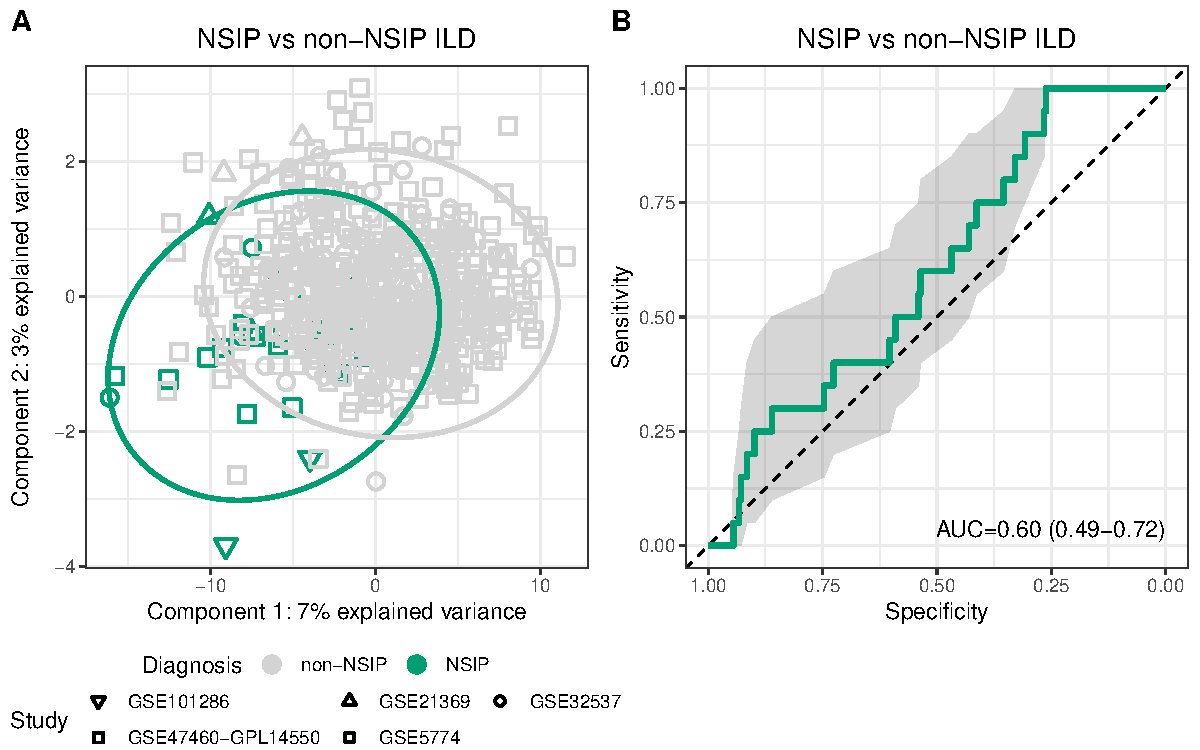
\includegraphics[width=0.9\linewidth,]{./Figures/SysReview/FigE5_NSIP} 

}

\caption[Model tuning]{\textbf{NSIP-specific classification model.} PLS projection of samples using the NSIP vs non-NSIP ILD model (A) and the AUC performance on held-out test datasets (B).}\label{fig:nsipmodel}
\end{figure}



\begin{figure}

{\centering 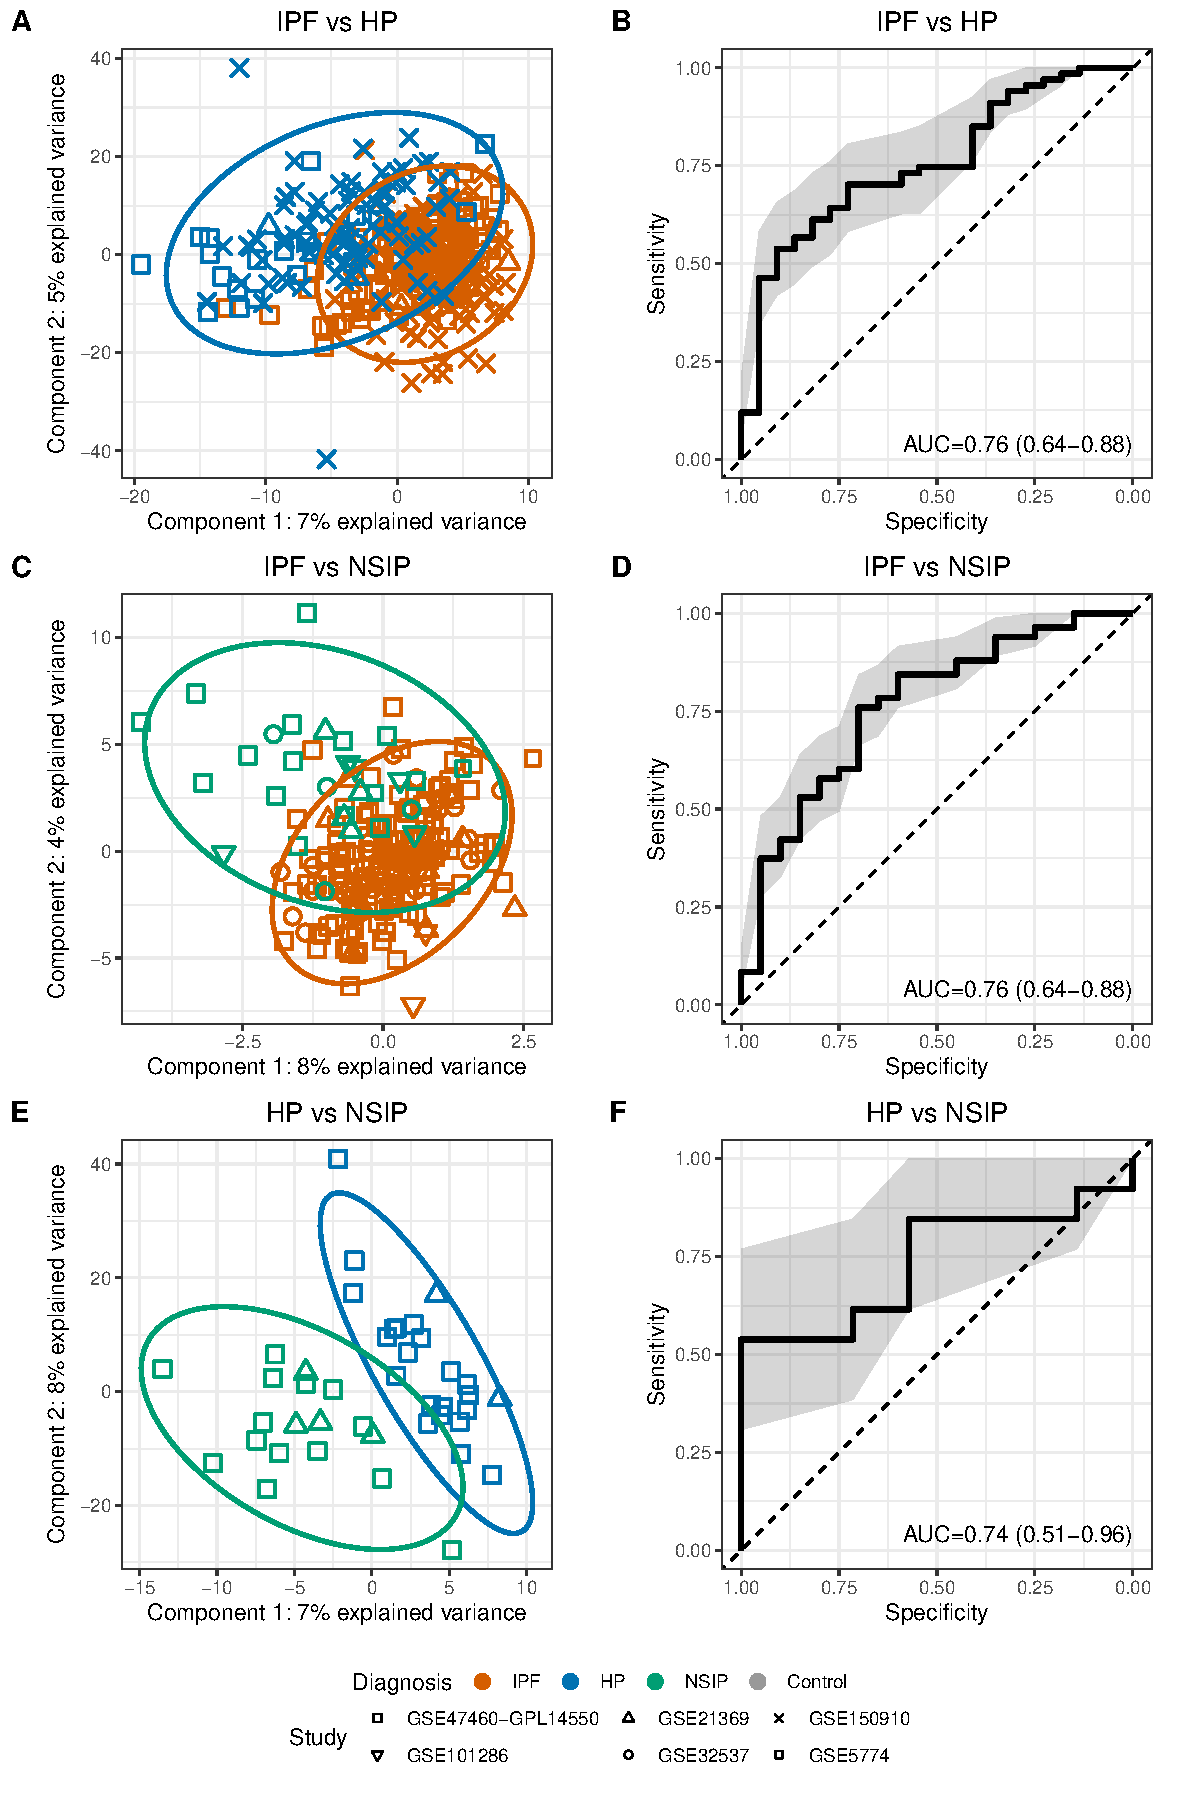
\includegraphics[width=0.8\linewidth,]{./Figures/SysReview/FigE6_ILDvsILD} 

}

\caption[Individual ILD vs ILD]{\textbf{Classification models differentiating between specific ILD subtypes.} PLS sample projections and held-out test set AUC performance for comparisons between IPF and HP (A, B), IPF and NSIP (C, D), and HP and NSIP (E, F).}\label{fig:ildvsildspecific}
\end{figure}

\newpage



\begin{figure}

{\centering 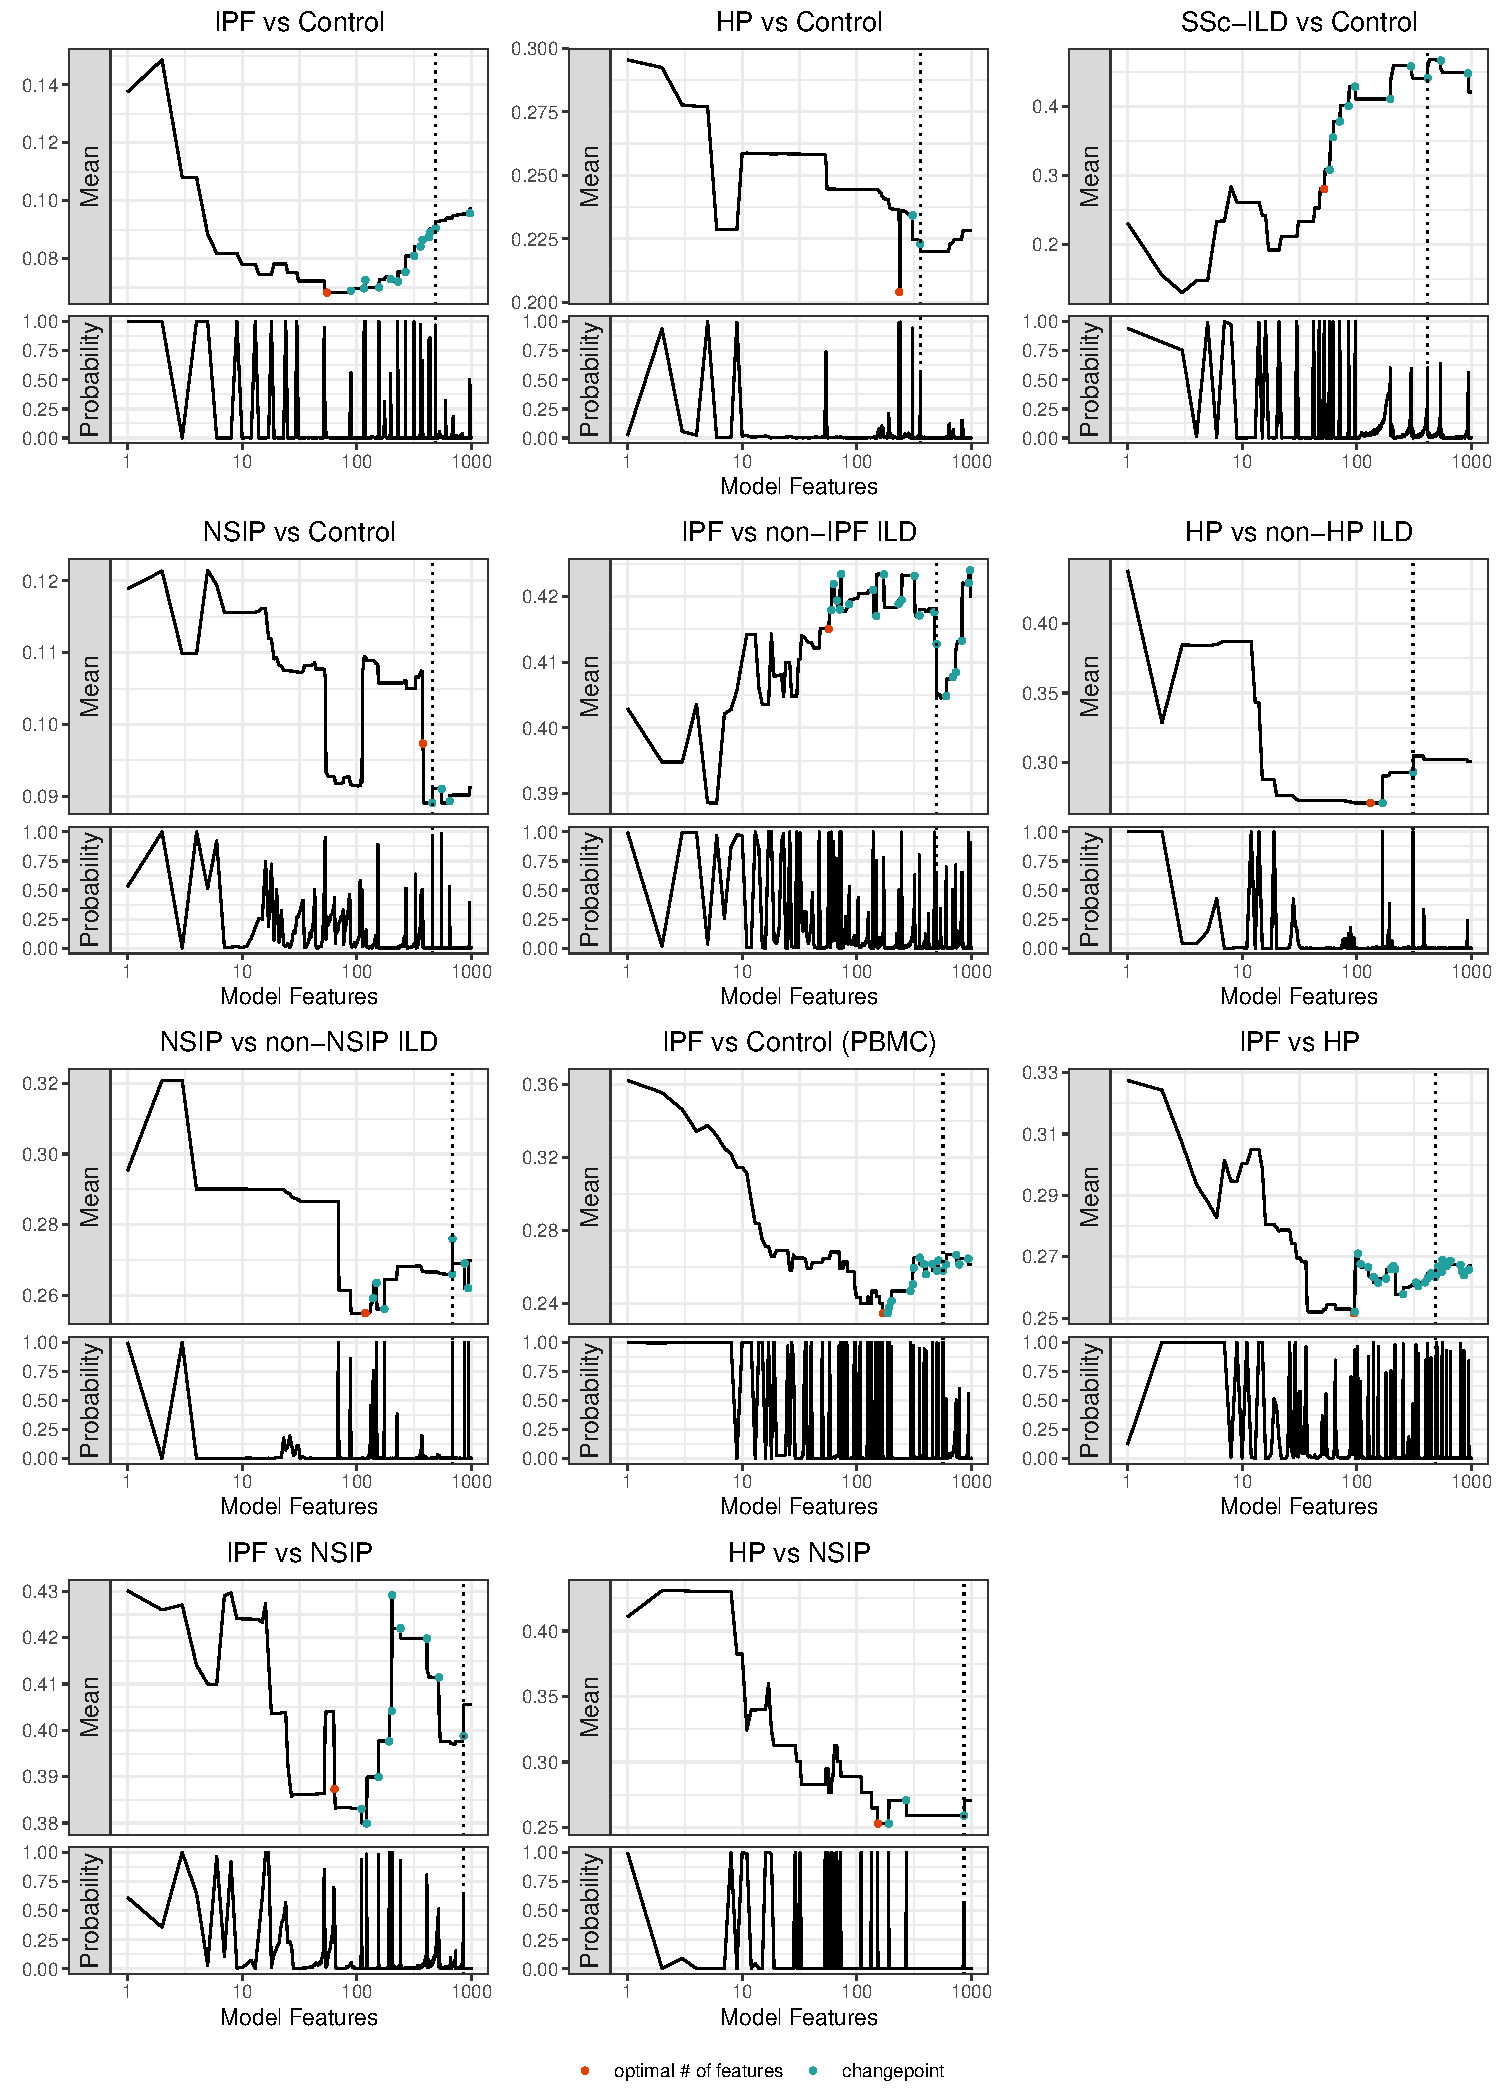
\includegraphics[width=0.8\linewidth,]{./Figures/SysReview/FigE7_bayes} 

}

\caption[Bayesian changepoint]{\textbf{Bayesian changepoint analysis to determine models with an ‘expanded’ number of features for the purpose of pathway analysis.} As the number of features is increased, the posterior mean (i.e.~an estimate of the BER given previous data and new data) is constant for certain ranges and does not increase until a threshold of features is passed; this is likely due to the addition of correlated features, which are not useful in the optimization of a classifier but are useful in strengthening the identification of relevant biological pathways. If we consider the BERs from the tuning grids to be a data series with an unknown number of blocks containing a constant mean, we can apply a Bayesian framework to determine `change points' (points likely to precede a change in BER) within the series, which were identified using a posterior probability threshold of 50\%.}\label{fig:bayes}
\end{figure}

\begin{singlespace}



\begingroup\fontsize{8}{10}\selectfont

\begin{longtable}[t]{>{\raggedright\arraybackslash}p{1.0in}>{\raggedright\arraybackslash}p{4.5in}c}
\caption{\label{tab:uppathways}\textbf{Top 10 up-regulated pathways in lung using genes from the expanded classification models for IPF, HP, NSIP, and SSc-ILD against Control.}}\\
\toprule
Direction & Pathway & FDR\\
\midrule
\endfirsthead
\caption[]{\label{tab:uppathways}\textbf{Top 10 up-regulated pathways in lung using genes from the expanded classification models for IPF, HP, NSIP, and SSc-ILD against Control.} \textit{(continued)}}\\
\toprule
Direction & Pathway & FDR\\
\midrule
\endhead

\endfoot
\bottomrule
\endlastfoot
IPF Up & REACTOME EXTRACELLULAR MATRIX ORGANIZATION & 1.81e-17\\
IPF Up & GOBP EXTERNAL ENCAPSULATING STRUCTURE ORGANIZATION & 1.16e-14\\
IPF Up & GOBP CELL ADHESION & 1.20e-14\\
IPF Up & REACTOME COLLAGEN DEGRADATION & 6.93e-13\\
IPF Up & REACTOME DEGRADATION OF THE EXTRACELLULAR MATRIX & 1.23e-12\\
\addlinespace
IPF Up & GOBP TISSUE MORPHOGENESIS & 1.38e-11\\
IPF Up & GOBP OSSIFICATION & 1.75e-10\\
IPF Up & GOBP ANIMAL ORGAN MORPHOGENESIS & 3.85e-10\\
IPF Up & GOBP GENERATION OF NEURONS & 4.57e-10\\
IPF Up & GOBP MESENCHYME DEVELOPMENT & 1.09e-09\\
\addlinespace
HP Up & GOBP POSITIVE REGULATION OF IMMUNE SYSTEM PROCESS & 1.43e-04\\
HP Up & REACTOME COLLAGEN DEGRADATION & 2.22e-04\\
HP Up & HALLMARK COAGULATION & 3.90e-04\\
HP Up & GOBP EXTERNAL ENCAPSULATING STRUCTURE ORGANIZATION & 2.05e-03\\
HP Up & GOBP TAXIS & 2.11e-03\\
\addlinespace
HP Up & GOBP MONONUCLEAR CELL DIFFERENTIATION & 2.65e-03\\
HP Up & GOBP IMMUNE EFFECTOR PROCESS & 2.66e-03\\
HP Up & GOBP REGULATION OF IMMUNE SYSTEM PROCESS & 3.26e-03\\
HP Up & REACTOME ASSEMBLY OF COLLAGEN FIBRILS AND OTHER MULTIMERIC STRUCTURES & 3.26e-03\\
HP Up & GOBP EXTRACELLULAR MATRIX DISASSEMBLY & 3.86e-03\\
\addlinespace
NSIP Up & GOBP EXTERNAL ENCAPSULATING STRUCTURE ORGANIZATION & 9.27e-15\\
NSIP Up & REACTOME COLLAGEN DEGRADATION & 1.19e-11\\
NSIP Up & REACTOME EXTRACELLULAR MATRIX ORGANIZATION & 1.40e-10\\
NSIP Up & REACTOME ASSEMBLY OF COLLAGEN FIBRILS AND OTHER MULTIMERIC STRUCTURES & 2.90e-10\\
NSIP Up & REACTOME COLLAGEN FORMATION & 3.21e-10\\
\addlinespace
NSIP Up & GOBP COLLAGEN FIBRIL ORGANIZATION & 4.52e-10\\
NSIP Up & REACTOME COLLAGEN BIOSYNTHESIS AND MODIFYING ENZYMES & 6.81e-10\\
NSIP Up & REACTOME COLLAGEN CHAIN TRIMERIZATION & 8.12e-10\\
NSIP Up & GOBP CELL DIVISION & 9.74e-10\\
NSIP Up & REACTOME DEGRADATION OF THE EXTRACELLULAR MATRIX & 1.13e-09\\
\addlinespace
SSc-ILD Up & GOBP EXTERNAL ENCAPSULATING STRUCTURE ORGANIZATION & 6.93e-11\\
SSc-ILD Up & HALLMARK EPITHELIAL MESENCHYMAL TRANSITION & 2.27e-08\\
SSc-ILD Up & REACTOME COLLAGEN DEGRADATION & 3.12e-08\\
SSc-ILD Up & REACTOME DEGRADATION OF THE EXTRACELLULAR MATRIX & 7.27e-08\\
SSc-ILD Up & REACTOME EXTRACELLULAR MATRIX ORGANIZATION & 3.59e-07\\
\addlinespace
SSc-ILD Up & REACTOME ASSEMBLY OF COLLAGEN FIBRILS AND OTHER MULTIMERIC STRUCTURES & 1.42e-06\\
SSc-ILD Up & GOBP EPITHELIUM DEVELOPMENT & 2.18e-06\\
SSc-ILD Up & GOBP CELL ADHESION & 2.45e-06\\
SSc-ILD Up & KEGG ECM RECEPTOR INTERACTION & 6.34e-06\\
SSc-ILD Up & GOBP CELL CELL SIGNALING & 6.34e-06\\*
\end{longtable}
\endgroup{}



\begingroup\fontsize{8}{10}\selectfont

\begin{longtable}[t]{>{\raggedright\arraybackslash}p{1.0in}>{\raggedright\arraybackslash}p{4.5in}c}
\caption{\label{tab:downpathways}\textbf{Top 10 down-regulated pathways in lung using genes from the expanded classification models for IPF, HP, NSIP, and SSc-ILD against Control.}}\\
\toprule
Direction & Pathway & FDR\\
\midrule
\endfirsthead
\caption[]{\label{tab:downpathways}\textbf{Top 10 down-regulated pathways in lung using genes from the expanded classification models for IPF, HP, NSIP, and SSc-ILD against Control.} \textit{(continued)}}\\
\toprule
Direction & Pathway & FDR\\
\midrule
\endhead

\endfoot
\bottomrule
\endlastfoot
IPF Down & GOBP TUBE MORPHOGENESIS & 2.19e-26\\
IPF Down & GOBP TUBE DEVELOPMENT & 1.25e-25\\
IPF Down & GOBP ANATOMICAL STRUCTURE FORMATION INVOLVED IN MORPHOGENESIS & 4.30e-25\\
IPF Down & GOBP BLOOD VESSEL MORPHOGENESIS & 5.06e-23\\
IPF Down & GOBP CIRCULATORY SYSTEM DEVELOPMENT & 5.82e-22\\
\addlinespace
IPF Down & GOBP VASCULATURE DEVELOPMENT & 8.67e-22\\
IPF Down & GOBP REGULATION OF CELL POPULATION PROLIFERATION & 1.01e-17\\
IPF Down & GOBP REGULATION OF LOCOMOTION & 1.28e-17\\
IPF Down & GOBP CELL MOTILITY & 6.52e-17\\
IPF Down & GOBP LOCOMOTION & 8.05e-15\\
\addlinespace
HP Down & GOBP TUBE MORPHOGENESIS & 2.60e-29\\
HP Down & GOBP TUBE DEVELOPMENT & 2.05e-28\\
HP Down & GOBP BLOOD VESSEL MORPHOGENESIS & 3.66e-26\\
HP Down & GOBP VASCULATURE DEVELOPMENT & 9.63e-25\\
HP Down & GOBP ANATOMICAL STRUCTURE FORMATION INVOLVED IN MORPHOGENESIS & 4.43e-24\\
\addlinespace
HP Down & GOBP CIRCULATORY SYSTEM DEVELOPMENT & 7.51e-22\\
HP Down & GOBP CELL MOTILITY & 1.31e-21\\
HP Down & GOBP REGULATION OF LOCOMOTION & 1.75e-18\\
HP Down & GOBP LOCOMOTION & 3.48e-17\\
HP Down & GOBP RESPONSE TO ENDOGENOUS STIMULUS & 5.28e-17\\
\addlinespace
NSIP Down & GOBP TUBE DEVELOPMENT & 1.08e-32\\
NSIP Down & GOBP TUBE MORPHOGENESIS & 1.06e-31\\
NSIP Down & GOBP BLOOD VESSEL MORPHOGENESIS & 9.59e-31\\
NSIP Down & GOBP VASCULATURE DEVELOPMENT & 3.12e-30\\
NSIP Down & GOBP CIRCULATORY SYSTEM DEVELOPMENT & 1.24e-29\\
\addlinespace
NSIP Down & GOBP ANATOMICAL STRUCTURE FORMATION INVOLVED IN MORPHOGENESIS & 4.54e-28\\
NSIP Down & GOBP REGULATION OF CELL POPULATION PROLIFERATION & 2.29e-20\\
NSIP Down & GOBP REGULATION OF MULTICELLULAR ORGANISMAL DEVELOPMENT & 1.28e-19\\
NSIP Down & GOBP CELL MOTILITY & 1.69e-19\\
NSIP Down & GOBP REGULATION OF LOCOMOTION & 4.61e-17\\
\addlinespace
SSc-ILD Down & GOBP TUBE DEVELOPMENT & 5.59e-18\\
SSc-ILD Down & GOBP VASCULATURE DEVELOPMENT & 9.46e-16\\
SSc-ILD Down & GOBP BLOOD VESSEL MORPHOGENESIS & 9.46e-16\\
SSc-ILD Down & GOBP RESPONSE TO ENDOGENOUS STIMULUS & 3.15e-15\\
SSc-ILD Down & GOBP CELL MOTILITY & 1.86e-14\\
\addlinespace
SSc-ILD Down & GOBP CIRCULATORY SYSTEM DEVELOPMENT & 4.92e-14\\
SSc-ILD Down & GOBP TUBE MORPHOGENESIS & 5.13e-14\\
SSc-ILD Down & GOBP LOCOMOTION & 7.41e-14\\
SSc-ILD Down & GOBP ANATOMICAL STRUCTURE FORMATION INVOLVED IN MORPHOGENESIS & 1.14e-13\\
SSc-ILD Down & GOBP POSITIVE REGULATION OF MULTICELLULAR ORGANISMAL PROCESS & 2.26e-13\\*
\end{longtable}
\endgroup{}



\begingroup\fontsize{8}{10}\selectfont

\begin{longtable}[t]{>{\raggedright\arraybackslash}p{1.0in}>{\raggedright\arraybackslash}p{4.5in}c}
\caption{\label{tab:ipfbloodpathways}\textbf{Top 10 up- and down-regulated pathways in IPF blood and PBMC using genes from the expanded classification models.}}\\
\toprule
Direction & Pathway & FDR\\
\midrule
\endfirsthead
\caption[]{\label{tab:ipfbloodpathways}\textbf{Top 10 up- and down-regulated pathways in IPF blood and PBMC using genes from the expanded classification models.} \textit{(continued)}}\\
\toprule
Direction & Pathway & FDR\\
\midrule
\endhead

\endfoot
\bottomrule
\endlastfoot
IPF Blood Up & REACTOME NEUTROPHIL DEGRANULATION & 6.87e-39\\
IPF Blood Up & REACTOME INNATE IMMUNE SYSTEM & 3.65e-34\\
IPF Blood Up & GOBP DEFENSE RESPONSE & 3.84e-19\\
IPF Blood Up & GOBP IMMUNE RESPONSE & 1.91e-14\\
IPF Blood Up & GOBP DEFENSE RESPONSE TO OTHER ORGANISM & 2.59e-13\\
\addlinespace
IPF Blood Up & GOBP INFLAMMATORY RESPONSE & 5.12e-13\\
IPF Blood Up & GOBP BIOLOGICAL PROCESS INVOLVED IN INTERSPECIES INTERACTION BETWEEN ORGANISMS & 8.43e-13\\
IPF Blood Up & GOBP REGULATION OF RESPONSE TO EXTERNAL STIMULUS & 1.10e-12\\
IPF Blood Up & GOBP INNATE IMMUNE RESPONSE & 3.03e-12\\
IPF Blood Up & GOBP POSITIVE REGULATION OF MULTICELLULAR ORGANISMAL PROCESS & 4.56e-11\\
\addlinespace
IPF PBMC Up & GOBP BIOLOGICAL PROCESS INVOLVED IN INTERSPECIES INTERACTION BETWEEN ORGANISMS & 2.05e-07\\
IPF PBMC Up & REACTOME NEUTROPHIL DEGRANULATION & 4.37e-07\\
IPF PBMC Up & GOBP DEFENSE RESPONSE & 1.89e-06\\
IPF PBMC Up & REACTOME INNATE IMMUNE SYSTEM & 1.10e-05\\
IPF PBMC Up & GOBP BONE RESORPTION & 1.89e-05\\
\addlinespace
IPF PBMC Up & GOBP REGULATION OF TRANSPORT & 2.99e-05\\
IPF PBMC Up & GOBP RESPONSE TO BACTERIUM & 3.56e-05\\
IPF PBMC Up & GOBP NEGATIVE REGULATION OF MULTICELLULAR ORGANISMAL PROCESS & 3.95e-05\\
IPF PBMC Up & GOBP DEFENSE RESPONSE TO OTHER ORGANISM & 7.56e-05\\
IPF PBMC Up & GOBP INNATE IMMUNE RESPONSE & 8.82e-05\\
\addlinespace
IPF Blood Down & GOBP T CELL DIFFERENTIATION & 4.02e-09\\
IPF Blood Down & GOBP RNA PROCESSING & 1.94e-08\\
IPF Blood Down & GOBP T CELL ACTIVATION & 7.68e-08\\
IPF Blood Down & GOBP MONONUCLEAR CELL DIFFERENTIATION & 2.57e-07\\
IPF Blood Down & GOBP LYMPHOCYTE ACTIVATION & 5.41e-07\\
\addlinespace
IPF Blood Down & GOBP ALPHA BETA T CELL ACTIVATION & 6.08e-07\\
IPF Blood Down & GOBP REGULATION OF IMMUNE SYSTEM PROCESS & 2.56e-06\\
IPF Blood Down & GOBP LEUKOCYTE DIFFERENTIATION & 6.59e-06\\
IPF Blood Down & REACTOME TRANSPORT OF MATURE MRNAS DERIVED FROM INTRONLESS TRANSCRIPTS & 1.17e-05\\
IPF Blood Down & GOBP ANTIGEN RECEPTOR MEDIATED SIGNALING PATHWAY & 1.62e-05\\
\addlinespace
IPF PBMC Down & REACTOME RNA POLYMERASE II TRANSCRIPTION & 6.53e-15\\
IPF PBMC Down & GOBP NEGATIVE REGULATION OF NUCLEOBASE CONTAINING COMPOUND METABOLIC PROCESS & 4.73e-07\\
IPF PBMC Down & GOBP NEGATIVE REGULATION OF RNA BIOSYNTHETIC PROCESS & 2.65e-06\\
IPF PBMC Down & GOBP NEGATIVE REGULATION OF BIOSYNTHETIC PROCESS & 3.90e-06\\
IPF PBMC Down & GOBP NCRNA METABOLIC PROCESS & 6.82e-06\\
\addlinespace
IPF PBMC Down & GOBP NCRNA PROCESSING & 1.32e-05\\
IPF PBMC Down & GOBP AMIDE BIOSYNTHETIC PROCESS & 1.25e-04\\
IPF PBMC Down & WP EXTRAFOLLICULAR AND FOLLICULAR B CELL ACTIVATION BY SARSCOV2 & 1.71e-04\\
IPF PBMC Down & GOBP ORGANONITROGEN COMPOUND BIOSYNTHETIC PROCESS & 2.81e-04\\
IPF PBMC Down & GOBP REGULATION OF CELLULAR MACROMOLECULE BIOSYNTHETIC PROCESS & 3.42e-04\\*
\end{longtable}
\endgroup{}



\begingroup\fontsize{8}{10}\selectfont

\begin{longtable}[t]{>{\raggedright\arraybackslash}p{1.0in}>{\raggedright\arraybackslash}p{4.5in}c}
\caption{\label{tab:ipfvsildpathways}\textbf{Top 25 up-regulated pathways using genes from the expanded IPF vs non-IPF ILD classification model.}}\\
\toprule
Direction & Pathway & FDR\\
\midrule
\endfirsthead
\caption[]{\label{tab:ipfvsildpathways}\textbf{Top 25 up-regulated pathways using genes from the expanded IPF vs non-IPF ILD classification model.} \textit{(continued)}}\\
\toprule
Direction & Pathway & FDR\\
\midrule
\endhead

\endfoot
\bottomrule
\endlastfoot
IPF vs ILD Up & GOBP CELL ADHESION & 2.28e-20\\
IPF vs ILD Up & REACTOME EXTRACELLULAR MATRIX ORGANIZATION & 2.65e-13\\
IPF vs ILD Up & HALLMARK EPITHELIAL MESENCHYMAL TRANSITION & 7.09e-13\\
IPF vs ILD Up & REACTOME COLLAGEN FORMATION & 2.95e-11\\
IPF vs ILD Up & GOBP EXTERNAL ENCAPSULATING STRUCTURE ORGANIZATION & 8.72e-11\\
\addlinespace
IPF vs ILD Up & GOBP CELL MOTILITY & 8.72e-11\\
IPF vs ILD Up & GOBP RESPONSE TO ENDOGENOUS STIMULUS & 2.92e-10\\
IPF vs ILD Up & REACTOME COLLAGEN BIOSYNTHESIS AND MODIFYING ENZYMES & 7.29e-10\\
IPF vs ILD Up & GOBP CELL CELL ADHESION & 5.89e-09\\
IPF vs ILD Up & REACTOME ASSEMBLY OF COLLAGEN FIBRILS AND OTHER MULTIMERIC STRUCTURES & 7.50e-09\\
\addlinespace
IPF vs ILD Up & GOBP COLLAGEN FIBRIL ORGANIZATION & 1.16e-08\\
IPF vs ILD Up & REACTOME COLLAGEN CHAIN TRIMERIZATION & 1.47e-08\\
IPF vs ILD Up & GOBP OSTEOBLAST DIFFERENTIATION & 2.05e-08\\
IPF vs ILD Up & GOBP ENZYME LINKED RECEPTOR PROTEIN SIGNALING PATHWAY & 2.05e-08\\
IPF vs ILD Up & GOBP OSSIFICATION & 4.63e-08\\
\addlinespace
IPF vs ILD Up & GOBP HOMEOSTATIC PROCESS & 6.20e-08\\
IPF vs ILD Up & GOBP TISSUE MORPHOGENESIS & 8.23e-08\\
IPF vs ILD Up & GOBP ANIMAL ORGAN MORPHOGENESIS & 1.40e-07\\
IPF vs ILD Up & GOBP CIRCULATORY SYSTEM DEVELOPMENT & 1.64e-07\\
IPF vs ILD Up & GOBP HEART DEVELOPMENT & 2.24e-07\\
\addlinespace
IPF vs ILD Up & REACTOME COLLAGEN DEGRADATION & 2.32e-07\\
IPF vs ILD Up & GOBP MUSCLE TISSUE DEVELOPMENT & 2.95e-07\\
IPF vs ILD Up & GOBP NEGATIVE REGULATION OF TRANSMEMBRANE RECEPTOR PROTEIN SERINE THREONINE KINASE SIGNALING PATHWAY & 2.99e-07\\
IPF vs ILD Up & GOBP LOCOMOTION & 4.04e-07\\
IPF vs ILD Up & GOBP MESENCHYME DEVELOPMENT & 4.08e-07\\*
\end{longtable}
\endgroup{}



\begingroup\fontsize{8}{10}\selectfont

\begin{longtable}[t]{>{\raggedright\arraybackslash}p{1.0in}>{\raggedright\arraybackslash}p{4.5in}c}
\caption{\label{tab:hpvsildpathways}\textbf{Top 25 up-regulated pathways using genes from the expanded HP vs non-HP ILD classification model.}}\\
\toprule
Direction & Pathway & FDR\\
\midrule
\endfirsthead
\caption[]{\label{tab:hpvsildpathways}\textbf{Top 25 up-regulated pathways using genes from the expanded HP vs non-HP ILD classification model.} \textit{(continued)}}\\
\toprule
Direction & Pathway & FDR\\
\midrule
\endhead

\endfoot
\bottomrule
\endlastfoot
HP vs ILD Up & HALLMARK INTERFERON GAMMA RESPONSE & 1.38e-36\\
HP vs ILD Up & HALLMARK INTERFERON ALPHA RESPONSE & 1.15e-22\\
HP vs ILD Up & GOBP DEFENSE RESPONSE & 1.15e-22\\
HP vs ILD Up & HALLMARK ALLOGRAFT REJECTION & 4.50e-22\\
HP vs ILD Up & REACTOME CYTOKINE SIGNALING IN IMMUNE SYSTEM & 3.55e-19\\
\addlinespace
HP vs ILD Up & GOBP IMMUNE RESPONSE & 5.59e-18\\
HP vs ILD Up & GOBP REGULATION OF T CELL ACTIVATION & 1.33e-15\\
HP vs ILD Up & GOBP REGULATION OF IMMUNE SYSTEM PROCESS & 1.65e-15\\
HP vs ILD Up & GOBP LEUKOCYTE CELL CELL ADHESION & 7.31e-15\\
HP vs ILD Up & GOBP POSITIVE REGULATION OF IMMUNE SYSTEM PROCESS & 1.16e-14\\
\addlinespace
HP vs ILD Up & GOBP REGULATION OF LYMPHOCYTE ACTIVATION & 1.32e-14\\
HP vs ILD Up & GOBP DEFENSE RESPONSE TO OTHER ORGANISM & 2.08e-14\\
HP vs ILD Up & GOBP CELL ACTIVATION & 4.62e-14\\
HP vs ILD Up & GOBP POSITIVE REGULATION OF CELL ACTIVATION & 4.70e-14\\
HP vs ILD Up & GOBP T CELL ACTIVATION & 7.82e-14\\
\addlinespace
HP vs ILD Up & GOBP REGULATION OF CELL ACTIVATION & 1.32e-13\\
HP vs ILD Up & GOBP BIOLOGICAL PROCESS INVOLVED IN INTERSPECIES INTERACTION BETWEEN ORGANISMS & 2.95e-13\\
HP vs ILD Up & GOBP LYMPHOCYTE ACTIVATION & 3.42e-13\\
HP vs ILD Up & GOBP POSITIVE REGULATION OF LYMPHOCYTE ACTIVATION & 6.79e-13\\
HP vs ILD Up & GOBP INNATE IMMUNE RESPONSE & 7.96e-13\\
\addlinespace
HP vs ILD Up & GOBP POSITIVE REGULATION OF LEUKOCYTE CELL CELL ADHESION & 9.34e-13\\
HP vs ILD Up & REACTOME ADAPTIVE IMMUNE SYSTEM & 1.01e-12\\
HP vs ILD Up & GOBP REGULATION OF CELL CELL ADHESION & 1.71e-12\\
HP vs ILD Up & GOBP INFLAMMATORY RESPONSE & 1.78e-12\\
HP vs ILD Up & REACTOME ANTIGEN PROCESSING CROSS PRESENTATION & 3.84e-12\\*
\end{longtable}
\endgroup{}



\begingroup\fontsize{8}{10}\selectfont

\begin{longtable}[t]{>{\raggedright\arraybackslash}p{0.8in}>{\raggedright\arraybackslash}p{4.5in}c}
\caption{\label{tab:upcell}\textbf{Top 10 up-regulated cell annotations in lung using genes from the expanded classification models for IPF, HP, NSIP, and SSc-ILD against Control.}}\\
\toprule
Direction & Cell & FDR\\
\midrule
\endfirsthead
\caption[]{\label{tab:upcell}\textbf{Top 10 up-regulated cell annotations in lung using genes from the expanded classification models for IPF, HP, NSIP, and SSc-ILD against Control.} \textit{(continued)}}\\
\toprule
Direction & Cell & FDR\\
\midrule
\endhead

\endfoot
\bottomrule
\endlastfoot
IPF Up & Basal Cells & 8.30e-32\\
IPF Up & Basal cells & 1.18e-20\\
IPF Up & HAY BONE MARROW STROMAL & 1.18e-20\\
IPF Up & AdvF (PI16+) & 8.46e-20\\
IPF Up & Myofibroblasts & 8.46e-20\\
\addlinespace
IPF Up & HE LIM SUN FETAL LUNG C1 SMG BASAL CELL & 2.28e-19\\
IPF Up & Fibroblasts & 2.40e-19\\
IPF Up & AdvF (SFRP2+) & 7.05e-19\\
IPF Up & Inflammatory fibroblast 3 & 7.05e-19\\
IPF Up & Inflammatory fibroblast 1 & 7.55e-18\\
\addlinespace
HP Up & Plasma cells & 4.54e-11\\
HP Up & Plasma & 8.02e-11\\
HP Up & Plasma Cells & 1.16e-08\\
HP Up & AIZARANI LIVER C38 RESIDENT B CELLS 3 & 3.47e-08\\
HP Up & AIZARANI LIVER C22 RESIDENT B CELLS 2 & 2.25e-07\\
\addlinespace
HP Up & AIZARANI LIVER C8 RESIDENT B CELLS 1 & 2.74e-07\\
HP Up & GAO LARGE INTESTINE ADULT CI MESENCHYMAL CELLS & 4.36e-07\\
HP Up & HAY BONE MARROW PLASMA CELL & 6.16e-07\\
HP Up & Melanocytes & 1.03e-06\\
HP Up & DURANTE ADULT OLFACTORY NEUROEPITHELIUM PLASMA CELLS & 1.14e-06\\
\addlinespace
NSIP Up & Plasma cells & 1.33e-25\\
NSIP Up & FAN EMBRYONIC CTX MICROGLIA 1 & 2.81e-23\\
NSIP Up & HE LIM SUN FETAL LUNG C2 PROMONOCYTE LIKE CELL & 5.51e-22\\
NSIP Up & ZHONG PFC C1 OPC & 4.32e-21\\
NSIP Up & MANNO MIDBRAIN NEUROTYPES HPROGFPM & 4.50e-20\\
\addlinespace
NSIP Up & MANNO MIDBRAIN NEUROTYPES HPROGFPL & 1.12e-19\\
NSIP Up & HE LIM SUN FETAL LUNG C5 PRO B CELL & 1.66e-19\\
NSIP Up & HE LIM SUN FETAL LUNG C4 CYCLING NK CELL & 8.34e-18\\
NSIP Up & FAN EMBRYONIC CTX NSC 2 & 3.45e-17\\
NSIP Up & HE LIM SUN FETAL LUNG C3 CYCLING DEFINITIVE ERYTHROBLAST & 1.41e-16\\
\addlinespace
SSc-ILD Up & Basal Cells & 3.07e-24\\
SSc-ILD Up & Basal cells & 1.40e-12\\
SSc-ILD Up & Myofibroblasts & 1.40e-12\\
SSc-ILD Up & Basal & 8.44e-12\\
SSc-ILD Up & TRAVAGLINI LUNG BASAL CELL & 2.25e-11\\
\addlinespace
SSc-ILD Up & Aberrant basaloid cells & 3.66e-11\\
SSc-ILD Up & TRAVAGLINI LUNG PROLIFERATING BASAL CELL & 4.71e-11\\
SSc-ILD Up & Proliferating Basal & 4.71e-11\\
SSc-ILD Up & Basal keratinocytes & 1.04e-09\\
SSc-ILD Up & Differentiating Basal & 1.47e-09\\*
\end{longtable}
\endgroup{}



\begingroup\fontsize{8}{10}\selectfont

\begin{longtable}[t]{>{\raggedright\arraybackslash}p{0.8in}>{\raggedright\arraybackslash}p{4.5in}c}
\caption{\label{tab:downcell}\textbf{Top 10 down-regulated cell annotations in lung using genes from the expanded classification models for IPF, HP, NSIP, and SSc-ILD against Control.}}\\
\toprule
Direction & Cell & FDR\\
\midrule
\endfirsthead
\caption[]{\label{tab:downcell}\textbf{Top 10 down-regulated cell annotations in lung using genes from the expanded classification models for IPF, HP, NSIP, and SSc-ILD against Control.} \textit{(continued)}}\\
\toprule
Direction & Cell & FDR\\
\midrule
\endhead

\endfoot
\bottomrule
\endlastfoot
IPF Down & Cap-B EC & 1.09e-58\\
IPF Down & Alveolar Epithelial Type 1 & 6.21e-54\\
IPF Down & TRAVAGLINI LUNG ALVEOLAR EPITHELIAL TYPE 1 CELL & 2.13e-53\\
IPF Down & Cap-A EC & 7.09e-44\\
IPF Down & AT1 Cells & 1.56e-42\\
\addlinespace
IPF Down & VE Capillary B & 1.93e-41\\
IPF Down & Alveolar cells type 1 & 2.90e-40\\
IPF Down & Art EC & 2.26e-38\\
IPF Down & MANNO MIDBRAIN NEUROTYPES HENDO & 2.40e-37\\
IPF Down & AT1 & 3.79e-37\\
\addlinespace
HP Down & Cap-B EC & 3.72e-60\\
HP Down & Cap-A EC & 6.01e-48\\
HP Down & MANNO MIDBRAIN NEUROTYPES HENDO & 8.09e-43\\
HP Down & VE Capillary A & 1.92e-41\\
HP Down & Ito cells & 8.16e-40\\
\addlinespace
HP Down & VE Capillary B & 1.34e-38\\
HP Down & Endothelial/Lymphatic Cells & 7.23e-38\\
HP Down & TRAVAGLINI LUNG ALVEOLAR EPITHELIAL TYPE 1 CELL & 2.81e-37\\
HP Down & Art EC & 4.02e-34\\
HP Down & Alveolar Epithelial Type 1 & 1.81e-32\\
\addlinespace
NSIP Down & Cap-B EC & 3.99e-75\\
NSIP Down & TRAVAGLINI LUNG ALVEOLAR EPITHELIAL TYPE 1 CELL & 5.22e-71\\
NSIP Down & Cap-A EC & 7.03e-64\\
NSIP Down & Alveolar Epithelial Type 1 & 2.49e-61\\
NSIP Down & Art EC & 6.05e-53\\
\addlinespace
NSIP Down & MANNO MIDBRAIN NEUROTYPES HENDO & 4.43e-52\\
NSIP Down & Endothelial/Lymphatic Cells & 8.04e-44\\
NSIP Down & Capillary Intermediate 1 & 9.40e-43\\
NSIP Down & Capillary & 8.06e-42\\
NSIP Down & AT1 Cells & 1.29e-39\\
\addlinespace
SSc-ILD Down & Cap-B EC & 8.98e-62\\
SSc-ILD Down & Cap-A EC & 1.13e-55\\
SSc-ILD Down & Capillary Intermediate 1 & 1.10e-43\\
SSc-ILD Down & Art EC & 2.13e-39\\
SSc-ILD Down & Endothelial/Lymphatic Cells & 2.87e-36\\
\addlinespace
SSc-ILD Down & Capillary & 1.82e-35\\
SSc-ILD Down & VE Capillary B & 2.24e-33\\
SSc-ILD Down & TRAVAGLINI LUNG CAPILLARY INTERMEDIATE 1 CELL & 1.64e-28\\
SSc-ILD Down & AIZARANI LIVER C10 MVECS 1 & 1.12e-27\\
SSc-ILD Down & VE Capillary A & 8.26e-27\\*
\end{longtable}
\endgroup{}

\end{singlespace}

\hypertarget{biclustering-1}{%
\subsection{Biclustering}\label{biclustering-1}}

In MoSBi (v1.4.0), biclusters are identified via biclustering algorithms (bimax, fabia, isa2, plaid, QUBIC) {[}\protect\hyperlink{ref-rose_mosbi_2022}{52}{]}. UnPaSt is an \href{https://github.com/ozolotareva/UnPaSt}{unconstrained version} of the method published in {[}\protect\hyperlink{ref-zolotareva_identification_2021}{53}{]}. Ensemble biclusters from the identified biclusters are determined through Louvain community aggregation, while a similar procedure was performed for UnPaSt biclusters using weighted gene co-expression network analysis. Biclusters were filtered to select for those enriched in specific lung disease groups (control, IPF, HP, NSIP, COPD). We also included CTD-ILD (including unspecified CTD-ILD subtypes, RA-ILD, SSc-ILD) and other ILD (acute interstitial pneumonia, COP, CPFE, DIP, IPF-acute exacerbation, RB-ILD, unknown fibrosis) samples in our biclustering analysis to increase the number of ILD samples; however, these were not used in filtering for biclusters enriched in specific disease groups. Final biclusters were named sequentially with an M- prefix if identified from MoSBi or a U- prefix if identified by UnPaSt.



\begin{figure}

{\centering \includegraphics[width=0.8\linewidth,]{./Figures/SysReview/FigE8_allbiclusters} 

}

\caption[All biclusters]{\textbf{Biclusters identified by MoSBi (A) and UnPaSt (B) unsupervised learning algorithms.} Displayed heatmaps show bicluster genes in the rows, with the columns showing separated bicluster and non-cluster samples.}\label{fig:biclusterall}
\end{figure}



\begin{figure}
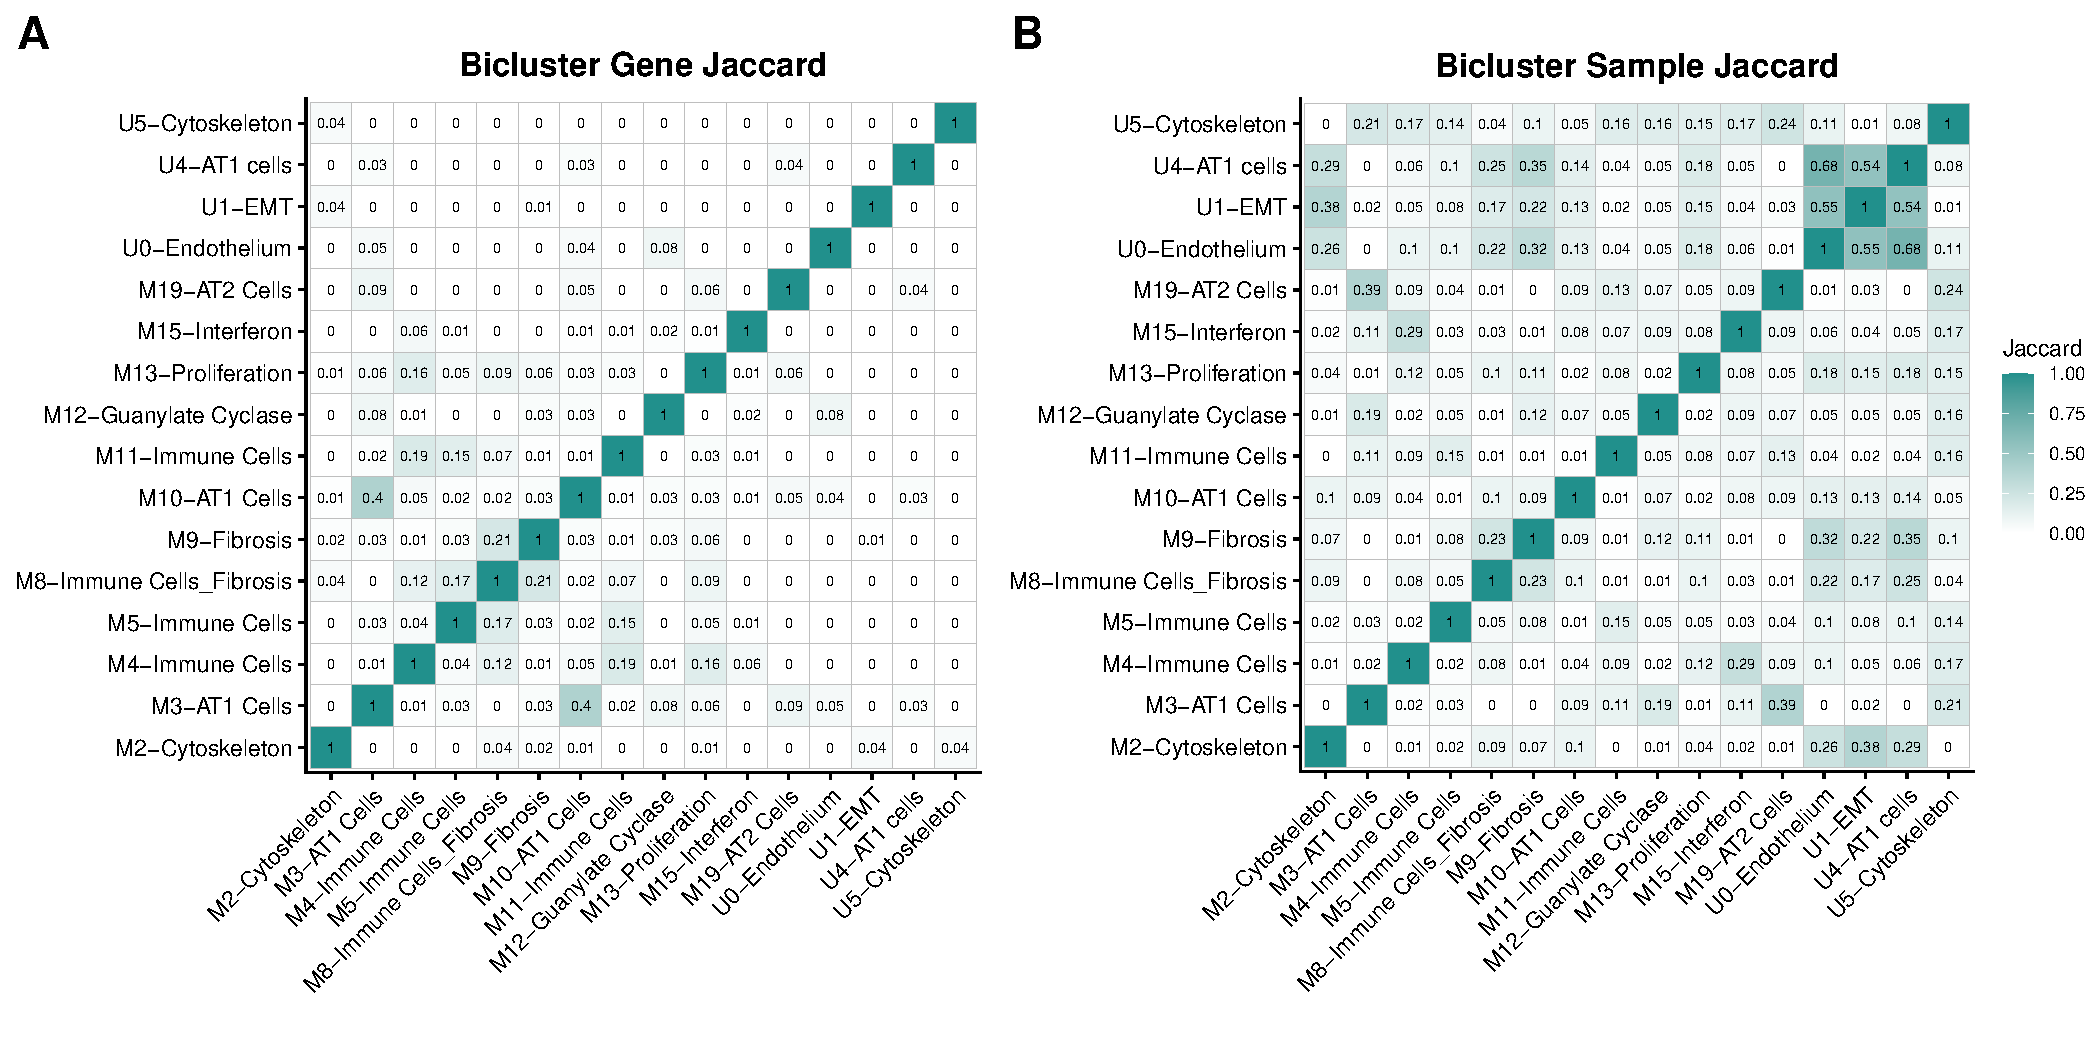
\includegraphics[width=1\linewidth,]{./Figures/SysReview/FigE9_biclusterjaccard} \caption[Bicluster similarity]{\textbf{Bicluster similarity scores.} Jaccard coefficients were calculated for genes (A) and samples (B) between each bicluster.}\label{fig:biclusterjaccard}
\end{figure}

\begin{singlespace}



\begingroup\fontsize{8}{10}\selectfont

\begin{longtable}[t]{>{\raggedright\arraybackslash}p{1in}>{\raggedright\arraybackslash}p{5in}}
\caption{\label{tab:biclusterGenes}\textbf{List of genes included in each bicluster.}}\\
\toprule
Bicluster & Genes\\
\midrule
\endfirsthead
\caption[]{\label{tab:biclusterGenes}\textbf{List of genes included in each bicluster.} \textit{(continued)}}\\
\toprule
Bicluster & Genes\\
\midrule
\endhead

\endfoot
\bottomrule
\endlastfoot
M2-Cytoskeleton & ABCC5, ABCD2, ABITRAM, ADORA2B, AHSA1, ALDH1A1, ALDH1L1, ALDH3A1, ALDH3B1, ALMS1, AMPD3, AP1M2, ARHGAP32, ATP12A, ATP2A2, ATP7B, ATP9A, B3GNT3, B4GALT4, B9D1, BAIAP3, BBS4, BBS9, BCAS1, BCAS3, BMPR1B, BPHL, C17orf75, C6, CCDC181, CCNO, CCP110, CDC14A, CDC14B, CDS1, CELSR1, CELSR2, CEP83, CERS6, CFAP20, CIB1, CLGN, CLMN, CLUAP1, CNTRL, CORO2B, CXCL6, CYP24A1, CYP2J2, DAPP1, DLEC1, DNAAF11, DNAH3, DNAH7, DNAH9, DNAI1, DNAJC10, DOC2A, DSP, DYNC2H1, DYNC2I1, DYNC2LI1, DYNLL1, DYNLT1, DZANK1, DZIP3, EFCAB2, EFHC1, EFNB3, EPB41L4B, EPHX2, ERBB2, ERBB4, FABP6, FAIM, FAM149A, FAM172A, FBXL2, FHOD3, FOXA1, FZD3, GALNS, GALNT3, GCLC, GET1, GNA14, GRAMD1C, GSTP1, H2BC5, HOOK1, HSP90AA1, HYDIN, IFT122, IFT140, IFT22, IFT56, IFT88, IGFBP2, IK, IL20RA, IL7, KATNIP, KCNN3, KIAA0319, KLF5, LGR4, LPAR3, LRBA, LRIG1, LRRC23, LTF, LZTFL1, MAK, MAP1A, MAPRE3, MATCAP2, MDM1, MIPEP, MOK, MORN1, MYB, NBEA, NEK1, NEK11, NEK2, NELL2, NET1, NME7, NUCB2, OSBPL3, P4HTM, PACRG, PASK, PCNX4, PHTF1, PIAS3, PIGR, PITPNM1, PLAAT2, PLAC8, PLPP2, PLS1, PRSS12, PSD3, PTPRF, PTPRN2, PTPRZ1, PZP, RARB, RCAN3, REEP1, RFX2, RFX3, RIPK4, RUVBL1, RUVBL2, SCPEP1, SIDT1, SLC22A4, SLC27A2, SLC2A1, SLC4A4, SLC4A8, SLC6A16, SMPD2, SNCAIP, SORBS2, SPA17, SPACA9, SPAG1, SPAG6, SPEF1, SPTBN2, SRGAP3, SRI, SSBP2, ST14, STAG3, STEAP3, STYK1, TASP1, TAX1BP1, TEKT2, TP53BP1, TP63, TP73, TPPP3, TRIM2, TRIM29, TRIM68, TRPV4, TSPAN1, TSPAN8, TSPYL4, TUBB4B, UFC1, USP2, USP21, VILL, WRAP53, XPNPEP3, ZDHHC13, ZMYND10, ZNF214\\
M3-AT1 Cells & AASS, AATK, ABCA3, ABCC8, ABHD6, ABLIM1, ACAT1, ACVRL1, ADARB1, ADGRL2, ADH1A, AGER, AGTPBP1, AGTR1, AJAP1, AKT3, ALDH1L1, ALDH6A1, AMOTL2, ANGPT1, ANKRA2, ANKS1A, ANXA3, AOC3, APC, APH1A, APLNR, APOL3, AQP4, ARHGAP44, ARHGEF12, ARHGEF17, ARPP19, ARRB1, ASAP2, ATP1A1, B3GALNT1, B3GNT2, BCAT2, BFAR, BMP6, BTN3A1, C1orf21, C21orf91, CA2, CA4, CACNA1D, CACNA2D2, CACNA2D3, CACNG4, CALCOCO1, CALCOCO2, CAMK2N1, CARMIL1, CAT, CAV2, CAVIN2, CCDC68, CCN5, CCNB1IP1, CCND3, CD247, CD36, CD55, CD93, CDC42BPA, CDH19, CDO1, CERS2, CETP, CFLAR, CHPT1, CHST1, CITED2, CLEC4M, CLIC5, CMKLR1, CNNM4, CNOT8, COLGALT2, COX7A1, CPT1A, CRIM1, CRMP1, CRTAC1, CRYAB, CST6, CTH, CTNNAL1, CTNNBIP1, CX3CR1, CXADR, CYP26B1, CYP3A5, CYP4B1, DAPK2, DCHS1, DDX60, DENND3, DHCR24, DLC1, DMPK, DNM2, DNM3, DNPEP, DOCK4, DOCK9, DPEP2, DST, DUOX1, DUSP7, EDIL3, EDN1, EDNRA, EDNRB, EFNA1, EGFL7, EGFR, ELMO1, ELOA, EML1, EMP2, ENG, ENTREP1, EPAS1, EPB41L2, EPB41L5, EPHB4, ERG, ERMP1, ETV1, ETV5, EXPH5, EZH1, F10, FADS3, FANCC, FAXDC2, FBLN5, FBXL4, FCHSD2, FEZ1, FGFR4, FHOD1, FLI1, FMO5, FOXO3, FRAS1, FRMD4A, FRY, FYN, FZD4, FZD5, GAB1, GAB2, GAL3ST1, GARRE1, GAS6, GCNT2, GFOD1, GHR, GIMAP4, GJA4, GLO1, GNLY, GPD1L, GPM6A, GRIA1, GSE1, GSTA4, GUCY1A2, GYPE, HEY1, HHEX, HIP1, HLX, HMGCS1, HOPX, HPCAL1, HPGD, HPS5, HSD11B2, HSD17B6, HSPA2, HYAL2, IFIT1, IL18R1, IL33, INPP5A, ITPKB, ITPRID2, JUP, KAT6B, KCNA4, KCNJ8, KCNS3, KDR, KLF11, KLF13, KLF2, KLRD1, LAMA3, LAMA5, LANCL1, LGR5, LHFPL6, LIFR, LLGL2, LMAN2L, LPIN2, LRCH1, LRRC1, LRRC32, LRRC36, LRRN3, MAL, MAPRE2, MATN3, MBIP, MCCC1, MFAP4, MFNG, MGLL, MINDY2, MKNK2, MME, MMUT, MOCS1, MPP3, MTSS1, MVB12B, MXD4, MYCT1, MYO5C, MYO9A, MYRF, NCALD, NCOA3, NDRG1, NDRG4, NEBL, NEDD4, NEDD4L, NEDD9, NEK7, NETO2, NHERF2, NINJ2, NOS1, NOTCH4, NPR1, NPR3, NR3C2, NRGN, NRN1, NRP1, OLFML2A, OSGIN2, P3H2, PAFAH1B1, PAPSS2, PARD3, PATJ, PCDH1, PCDH12, PCTP, PDCL, PDE1C, PDE8B, PDGFB, PDGFRA, PDK2, PDK4, PDZD2, PGAP2, PGC, PGM1, PGR, PHACTR2, PHLDB1, PIK3C2B, PIK3IP1, PIK3R1, PIP5K1B, PKIA, PKN1, PLA1A, PLA2G4C, PLAAT3, PLAG1, PLCE1, PLEKHA1, PLLP, PLXNA2, PLXND1, PMM1, PNMT, PON2, PPFIBP1, PPL, PPP2R5A, PRDX6, PRKAR2B, PRKCZ, PRKD1, PRX, PTGDR, PTH1R, PTPN12, PTPRB, PXMP4, QKI, RAB17, RALA, RAMP2, RAMP3, RAPGEF4, RASSF8, RBMS2, RBMS3, RECK, RFC1, RGS9, RIDA, RIN2, RMND5A, RNF144A, ROBO4, ROR1, RRAS, RUNX1T1, RUSC2, RXRG, S1PR1, SACM1L, SASH1, SCNN1A, SECISBP2L, SEMA3B, SEMA3E, SEMA3G, SENP7, SEPTIN4, SGCG, SLC12A4, SLC1A1, SLC35A1, SLC39A8, SLCO2A1, SLCO4A1, SLIT2, SMPD1, SOX13, SPRED2, SPRY2, SPRYD7, SPTBN1, SREBF2, ST7, STARD13, STX12, STX3, STXBP6, SVEP1, SYNE1, SYT17, TACC1, TACC2, TAL1, TBC1D4, TBX2, TBX3, TBX5, TCF21, TEAD1, TEK, TGFBR3, THBD, TIE1, TIMP4, TJP2, TLE1, TMEM100, TMEM109, TMEM140, TMEM41B, TMEM50B, TMEM74B, TMEM87A, TMEM97, TMOD1, TMOD2, TMT1A, TNFSF10, TNNC1, TNS1, TNS2, TOR1AIP2, TPST2, TRAK2, TRIB2, TRIM24, TRIP10, TSPAN12, TSPAN13, TSPAN15, TSPAN9, TTN, TUFT1, UBA7, UNC13B, USP13, UXS1, VAMP5, VEGFA, VEGFC, VGLL3, VIPR1, VWF, WASF3, WFDC1, WFS1, WWC1, YES1, ZBTB16, ZFYVE9, ZHX3, ZKSCAN3, ZNF106, ZNF135, ZNF22, ZSCAN31, ZXDC\\
M4-Immune Cells & ABCC3, ABCG1, ACAA1, ACAP1, ACO1, ACOT13, ACOT7, ACP2, ACP5, ADA, ADAM17, ADAP2, ADCY7, ADGRE2, ADSL, ADTRP, AGA, AGPS, AIM2, AKR1A1, AKR1B1, ALAS1, ALOX5, ALOX5AP, ANPEP, AOAH, APBB1IP, APH1A, APMAP, APOL1, APOL2, APOL3, AQP9, ARAP1, ARHGAP25, ARHGDIB, ARHGEF1, ARL6IP5, ARRB2, ASF1B, ASPM, ATG3, ATG7, ATIC, ATP2C1, ATP6V0B, ATP6V0D1, ATP6V1B2, ATP6V1C1, ATP6V1E1, ATP6V1F, AURKA, AVPI1, BAX, BCL11B, BCL2A1, BHLHE41, BIN2, BLM, BLNK, BLVRA, BMP2K, BST1, BTN2A2, BTN3A1, BUB1, C1QB, C3AR1, CASP1, CASP4, CASP5, CAT, CCDC88A, CCL19, CCNA2, CCR1, CCRL2, CD163, CD247, CD300A, CD3E, CD4, CD47, CD48, CD52, CD6, CD83, CD84, CD8A, CEP55, CHST11, CIITA, CLCN7, CLEC2D, CLEC7A, CLIP4, CMKLR1, COMMD9, CORO1A, CORO1B, CORO1C, CPVL, CR1, CRLF3, CSF1R, CTSC, CTSL, CTSS, CXCL10, CXCL9, CYRIA, CYRIB, CYTH4, DAPP1, DCK, DCSTAMP, DENND5A, DIAPH1, DLGAP5, DNASE2, DOK2, DPEP2, DRAP1, DUSP10, ECHDC1, EDEM2, EIF4E2, ELOVL1, EML4, EPB41L3, ERO1A, ETHE1, EVI2B, FAR2, FBP1, FCER1G, FIG4, FLOT2, FMNL1, FUCA1, FUT7, FXYD5, GAA, GALE, GALNT12, GCHFR, GGA2, GLB1, GLRX, GLUL, GM2A, GMIP, GNA15, GNG5, GNPDA1, GPA33, GPNMB, GPR132, GPR137B, GPR171, GPR18, GPR65, GPSM3, GSAP, GSTO1, GUSB, GYG1, HERC5, HEXB, HK3, HLA-DMB, HLA-G, HMGCL, HMOX1, HNMT, HPS5, HSD17B14, HSD17B4, HTATIP2, IDH2, IFFO1, IFI35, IFI6, IL12RB1, IL17RA, IL18, IL21R, IL2RB, IL32, INPP5B, INPP5D, IRAK4, IRF1, ITGAE, ITGAL, ITGAM, ITGB2, ITGB7, ITPK1, JAK3, JPT1, KCNAB2, KIF11, KIFC1, KYNU, LACTB2, LAP3, LAPTM5, LASP1, LAT2, LCP1, LGALS3, LGALS3BP, LGALS9, LGMN, LHFPL2, LILRB2, LILRB5, LIMK1, LIPA, LPCAT1, LRP1, LSM6, LTA4H, LY6E, LY9, LY96, MAFB, MAN2B1, MANBA, MAP4K1, MAPK13, MAPK14, MAPKAPK3, MARCO, MCM5, MDH1, ME2, MEFV, MELK, MFNG, MGAT1, MGAT4A, MICAL1, MICB, MITF, MKI67, MLX, MMD, MR1, MREG, MRPS15, MS4A4A, MSR1, MTMR14, MX1, MYD88, MYO5A, NAAA, NAGA, NAPA, NCF2, NCKAP1L, NEU1, NFE2L3, NFYC, NOP10, NPC1, NPC2, NUP210, OAS1, OAS2, OASL, OSTF1, PADI2, PARP12, PCK2, PCMT1, PCOLCE2, PDCD1LG2, PDE1B, PEPD, PFKFB4, PGD, PIK3CD, PLA2G7, PLAAT4, PLCL2, PLD3, PLEKHB2, PLIN2, PLK1, PLOD3, PLXNC1, PNPLA6, POP4, PPARG, PPT1, PRIM1, PRKAG1, PRKCD, PRSS21, PSD4, PSMA4, PSMA5, PSMB8, PSTPIP2, PTAFR, PTGER2, PTGER4, PTPN22, PTPN6, PTPRC, PTPRO, PXMP4, PYCARD, PYGL, RAB20, RAB32, RAD51AP1, RBP4, RFX5, RMC1, RMDN3, RNFT1, RNH1, RPS6KA1, RRAGC, RRAGD, RRM2, SCCPDH, SCP2, SCPEP1, SDHB, SECTM1, SELPLG, SEMA4A, SEMA4D, SERPINA1, SHTN1, SIGLEC7, SIRPG, SKAP1, SLA, SLAMF7, SLAMF8, SLC16A3, SLC16A6, SLC25A20, SLC31A2, SLC47A1, SLC50A1, SLC7A7, SLC9A1, SLCO2B1, SNX10, SP110, SP140, SP140L, ST3GAL6, STAC, STAT1, SYK, TAPBP, TBC1D31, TBXAS1, TGFBI, THEMIS2, TKT, TLR1, TLR4, TMEM104, TMEM140, TNF, TNFAIP2, TNFRSF1B, TPK1, TPP1, TPX2, TRAF1, TREM1, TREM2, TRIM14, TRIM21, TRPM2, TRPV2, UBA7, UTP18, VAMP8, VASH1, VASP, VAT1, VAV1, VPS26C, VPS37C, VPS8, WARS1, WIPF1, XRCC4, ZCCHC2, ZNF589\\
M5-Immune Cells & ABCE1, ABCF2, ADA, ADAM17, ADAM19, ADAM8, ADAMTS1, ADAMTS3, ADGRE2, ADGRE3, ADGRG1, ADM, AKAP12, AMD1, AMPD2, ANK2, ANXA1, AP1AR, APOBEC3B, AQP9, ARC, ARFGAP3, ARG2, ARHGDIA, ARID5B, ARPC5L, ATF3, ATG101, ATP1B3, B4GALT5, BACH1, BAHD1, BAZ1A, BCL2A1, BCL2L1, BHLHE40, BIRC3, BTG3, BYSL, BZW2, CASP4, CASP5, CBLB, CCDC59, CCNH, CCNL1, CCR1, CCT2, CCT5, CD83, CD93, CDA, CDC37L1, CDC42EP4, CEACAM1, CEBPB, CFLAR, CH25H, CHD1, CHD7, CHIC2, CHSY1, CRY1, CSF3, CSRP2, CST7, CX3CL1, CXCL1, CXCL2, CXCL8, CYRIA, DACT1, DENND5A, DEPP1, DGKD, DIAPH1, DLC1, DNAJB1, DNAJB5, DPH2, DSE, DUSP2, DUSP4, DUSP5, DUSP7, DYRK3, E2F3, EIF1B, EIF2S2, EIF3B, EML4, EPHA2, ETF1, FAM135A, FAS, FES, FFAR2, FGA, FJX1, FKBP1A, FLOT1, FNDC4, FOSB, FST, FURIN, GABPB1, GADD45A, GARS1, GATA6, GCA, GEM, GJA1, GNA15, GNL2, GPR132, GPR183, HAL, HAT1, HIVEP1, HIVEP2, HMOX1, HSPA9, HSPB8, IER3, IL10, IL18R1, IL18RAP, IL1R1, IL1R2, IL1RAP, IL4R, IL6, IL6ST, IRAK3, IRF1, ITGA2, ITGA5, ITPKC, IVNS1ABP, JMJD1C, JOSD1, KCNK1, KDM6B, KLHL2, KPNA2, KPNA4, KRAS, LAMC2, LDLR, LIF, LILRB2, LIMK2, LRRC32, LRRC59, MAFF, MAFG, MAK16, MAP3K8, MAPK1IP1L, MAT2A, MGAM, MMP19, MPHOSPH6, MTMR6, MX2, MYC, NAB1, NAT10, NDRG1, NDUFAF4, NDUFS2, NFATC1, NFIL3, NFKB1, NNMT, NOL11, NOLC1, NOP2, NOP56, NPC1, NRIP1, NXT1, ODC1, OSGIN2, OSMR, OTUD4, PADI4, PAFAH1B1, PAK1IP1, PDE4B, PER2, PEX5, PFKFB3, PGM3, PHC2, PHLDA1, PHLDA2, PI3, PIM1, PISD, PLIN2, PLPP3, PLSCR1, POP1, PPIF, PPP1R10, PPRC1, PRDM1, PSME3, PSME4, PTGER2, PTGS2, PTPN12, PUM3, PUS7, PVR, RAB27A, RAPGEF4, RBM28, RCAN1, RELB, RGS16, RHOH, RIPK2, RIPOR2, RND1, RND3, RRAD, RRAGC, RRP12, RRP9, RRS1, RUNX1, S100A12, S100A8, S1PR1, SAMD4A, SAMSN1, SEC24A, SELE, SEMA4A, SEMA7A, SERPINB1, SERPINB8, SERPINB9, SERPINE1, SERTAD2, SGK1, SKIL, SLC16A3, SLC16A6, SLC19A2, SLC25A32, SLC25A44, SLC39A14, SLC3A2, SLC7A1, SLCO4A1, SOCS1, SOCS2, SOCS3, SOX17, SPRY2, SPSB1, SRF, SRSF7, SSH1, ST3GAL1, STAT4, STRAP, STX12, SYNJ2, TANK, TBK1, TEAD4, TES, TEX30, TFPI2, THBD, TIMM17A, TIPARP, TJP2, TLR4, TNFAIP2, TNFAIP3, TNFAIP6, TNFRSF10B, TNFRSF10C, TNFRSF11B, TNFRSF12A, TNFRSF1B, TNIP2, TOP1, TP53BP2, TRIB1, TRIP10, TUBB2A, UAP1, UGCG, USP10, USP15, UTP11, UTP18, UTP20, UTP3, VASP, VCPKMT, VDR, VEGFC, VNN2, WDR74, YBX3, YES1, YRDC, ZFAND5, ZFC3H1, ZNF267\\
M8-Immune Cells\_Fibrosis & AARS1, ABCD2, ACAP1, ADA, ADAM12, ADAM19, ADAM23, ADAM8, ADAMTS1, ADRA2A, AGA, AIM2, AKAP12, ALDH1A3, ALDH1B1, ALG6, ALG8, AMPD3, ANK2, ANKRD49, AOC1, ARC, ARFGAP3, ARG2, ARHGAP25, ARHGDIB, ARID5B, ARPC5L, ASCC3, ASPM, ATF7IP, ATG101, ATP1B2, ATP1B3, ATP2A3, AURKA, B4GALT5, BACE2, BCL11A, BCL11B, BHLHE41, BIRC3, BLM, BLNK, BMP2K, BRCA2, BTN2A2, BTN3A1, BUB1, BYSL, C11orf24, C15orf39, C1S, C3, C7, CADPS, CARD8, CASP3, CBLB, CCDC69, CCL19, CCL7, CCL8, CCNA2, CCNB1, CCND2, CCNH, CD19, CD247, CD27, CD3E, CD48, CD6, CD69, CD79A, CD79B, CD84, CD8A, CDC20, CDK14, CDKN2A, CDKN3, CENPF, CEP55, CH25H, CHD1, CHD7, CHL1, CHST15, CHSY1, CKAP2, CLEC2D, CLSTN3, CLU, CNTRL, COCH, COL15A1, COL18A1, CORO1A, CR1, CRLF3, CSF3, CSGALNACT1, CST7, CSTF2T, CTSK, CXCL1, CXCL12, CXCL13, CXCL6, CXCR4, CYP24A1, CYRIA, CYTH4, CYTIP, CYTL1, DAPP1, DCLK1, DENND1B, DGKA, DIO2, DKK1, DLGAP5, DNAJB5, DNAJC10, DOK5, DUSP2, DUSP4, DUSP5, DYRK3, E2F3, E2F5, EAF2, EDEM1, EHMT1, ELK3, ESR2, EVI2B, EXO1, FAM98A, FAN1, FBL, FBLN1, FBLN2, FBXW7, FHL2, FICD, FILIP1L, FJX1, FMNL1, FMO1, FNDC4, FOSB, FOXM1, FRZB, FST, FUT7, FUT8, FXYD5, FZD10, FZD3, GADD45A, GARS1, GEM, GMDS, GMIP, GNAO1, GP1BA, GPR132, GPR171, GPR18, GPR183, GPSM3, GPX7, GRAMD4, H1-10, H2BC5, HAAO, HDAC9, HERPUD1, HIVEP1, HIVEP2, HYOU1, IARS1, ICAM3, IDE, IDH2, IER3, IGF1, IGFBP5, IL10, IL12RB1, IL21R, IL2RA, IL2RB, IL6, INPP5D, IPCEF1, IRAK4, IRF4, ITGA6, ITGA7, ITGAL, ITGB7, ITPKC, JAK3, JMJD1C, JOSD1, KCND3, KCNN3, KDM6B, KIF11, KIF20A, KIF20B, KIFC1, KLF12, KNTC1, KPNA2, LAMP5, LAX1, LEF1, LIF, LIMK1, LOXL2, LTBP1, LTF, LY9, LY96, MAFF, MAK16, MANF, MAP4K1, MAPK1IP1L, MAT2A, MATN2, MCM5, MCM6, MDM1, MEF2C, MELK, MEOX1, METTL18, MIEF1, MKI67, MLEC, MMP10, MMP11, MMP19, MMP7, MMP9, MX2, MYC, MYO5A, MYRIP, MZB1, NAP1L4, NCOA3, NEK2, NFATC1, NFE2L3, NFIL3, NFKB1, NNMT, NOL8, NOLC1, NOP2, NOP56, NPAT, NR4A3, NRIP1, NT5E, NUCB2, NUP210, NXT1, OSBPL3, OSMR, OXCT1, P2RX1, PACS1, PAICS, PASK, PCNX2, PCSK1, PDE1A, PDE2A, PDE4B, PDGFRL, PDIA4, PDIA6, PDK1, PDLIM3, PFKFB3, PHLDA1, PHTF2, PI3, PIK3CD, PIM1, PLA2G2A, PLAU, PLCG2, PLCL2, PLK1, PLPP3, PLVAP, PLXDC1, PLXNC1, PMEPA1, PNOC, PPAT, PPIF, PPRC1, PRDM1, PRKACB, PRKD2, PSD4, PTGDR, PTP4A3, PTPN22, PTPRC, PYGM, RAD17, RANBP6, RARRES1, RASGRP3, RASSF2, RCAN1, RELB, RELN, RFX5, RGS1, RHOH, ROBO1, RPL3, RPL36, RPL5, RPS6, RRM2, RRP12, RRS1, SACS, SAMSN1, SCARA3, SCG5, SDC1, SDF2L1, SDK2, SEC24A, SEC24D, SEC61B, SEL1L, SEL1L3, SELE, SEMA4D, SEMA7A, SERPINA5, SERPINB9, SERPINE1, SERPINI1, SERTAD2, SFRP1, SHMT2, SIDT1, SIRPG, SKAP1, SLAMF7, SLC1A4, SLC25A12, SLC25A32, SLC25A44, SLC26A4, SLC2A1, SLC35B1, SLC38A1, SLC39A14, SLC50A1, SLC7A1, SLN, SMO, SND1, SOCS1, SOCS3, SOS1, SP110, SP140, SP140L, SPP1, SPRY1, SPSB1, SPTBN2, SRF, SRM, SRPRB, SSPN, SSR3, ST3GAL1, ST6GAL1, ST8SIA1, STAB2, STAG3, STAT4, STIL, SULF1, SV2B, SYK, SYNJ2, TATDN2, TCN1, TDO2, TF, THEMIS2, TMEM176A, TMEM208, TNFAIP6, TNFRSF10B, TNFRSF17, TNFRSF1B, TNN, TOP2A, TP63, TPX2, TRAF1, TRAF3, TRAF5, TRAM2, TRIB1, TRPM2, TTC3, TTK, TUBB2A, TUT4, TWIST1, TYMS, UAP1, UGCG, UGT8, UTP3, VAV1, VILL, VPS13C, WDR74, WIPF1, YRDC, ZBTB24, ZNF107, ZNF580, ZNF671\\
\addlinespace
M9-Fibrosis & AARS1, ABCA8, ABLIM3, ACOX2, ACTN1, ADA, ADAM12, ADAM19, ADAM23, ADAMTS1, ADAMTS12, ADAMTS2, ADAMTS3, ADCY2, ADCY3, ADD2, ADGRL3, ADRA2A, ADRA2C, ALDH1A2, ALDH1A3, ALDH1B1, ANK2, ANTXR1, ANXA6, AOPEP, APLNR, AQP7, ARID5B, ARL1, ASPN, ATP1A2, ATP1B2, ATP2A2, BACE2, BAX, BCHE, BCL9, BMP1, BMP4, BNC1, BNC2, C11orf24, C1R, C1S, C3, C7, CA11, CA3, CADPS, CALB2, CASQ2, CCN3, CCN5, CCND2, CD19, CD27, CD34, CD4, CD79A, CD79B, CDH2, CDH6, CDK4, CDKN2A, CDON, CEMIP, CEP68, CFI, CHRNB1, CHST15, CKMT2, CLDN1, CLDN15, CLSTN3, CLTCL1, CLU, CNTFR, COCH, COL15A1, COL18A1, COL4A2, COL5A2, COMP, COX7A1, CREB3L1, CRYAB, CSGALNACT1, CSPG4, CSRP1, CSRP2, CST5, CTSF, CTSK, CUL7, CXCL12, CXCL13, CYP1B1, CYP24A1, CYP26B1, CYTL1, DAAM2, DACT1, DCBLD2, DCHS1, DCLK1, DCN, DDB2, DDR2, DGKA, DIO2, DKK3, DMPK, DNAJB5, DOCK3, DOK5, DPT, DPYSL3, DST, DTNA, DZIP1, ECM1, ECM2, EDIL3, EIF5A2, ELN, ENAH, ENPP2, EPHA3, ESR1, ESR2, EXTL2, F10, F13A1, FADS2, FAM98A, FAP, FAT1, FBLN1, FBLN2, FBN2, FBXW7, FEZ1, FHL2, FILIP1L, FJX1, FKBP14, FMO1, FNDC4, FOLR2, FRZB, FST, FUT8, FZD10, FZD7, GADD45A, GALNT1, GARS1, GAS1, GAS6, GEM, GHR, GLT8D2, GMDS, GNAO1, GPI, GPSM2, GPX7, GREB1, GSN, GUCY1A1, GUCY1B1, HAAO, HDAC9, HEY2, HSPA12A, HSPB7, HTR2B, IGF1, IGFBP2, IGFBP3, IGFBP5, IL1R1, IRF4, ISLR, ITGA6, ITGA7, ITGAV, ITGBL1, ITIH5, JAG1, JPH2, KALRN, KAT2A, KCNA5, KCND3, KCNMA1, KCNN3, KDELR3, KLF12, KLHL3, LAMP5, LAX1, LEF1, LHX6, LILRB5, LIMA1, LIMK1, LOXL2, LRP1, LRRC17, LTBP1, MACROH2A2, MAF, MAN1C1, MANF, MAP1A, MAP4K4, MATN2, MCAM, MCM6, MEF2C, MEGF8, MEOX1, MEST, MFAP2, MFAP4, MLXIP, MMD, MMP10, MMP11, MMP14, MMP7, MOXD1, MSX2, MYLK, MYO1D, MYRIP, MZB1, NAV3, NDRG3, NET1, NFIB, NIBAN1, NID2, NLGN1, NMNAT2, NNMT, NOVA1, NOX4, NR2F2, NR5A2, NT5DC3, NT5E, NTRK3, NUAK1, OAT, OLFM1, OMD, OXCT1, P4HA2, PACS1, PALLD, PAMR1, PBX1, PCNX2, PCSK1, PDE10A, PDE1A, PDE1C, PDE2A, PDGFC, PDGFD, PDGFRL, PDIA4, PDIA6, PDK1, PDLIM3, PDLIM5, PDLIM7, PDZRN3, PDZRN4, PGR, PIGK, PKD2, PLA2G2A, PLA2R1, PLAU, PLIN1, PLIN3, PLN, PLOD1, PLOD3, PLPP1, PLPPR4, PLVAP, PLXDC1, PMEPA1, PNOC, PPFIA2, PPIC, PPP1R12B, PRCP, PRKAA2, PRKAB2, PRKAR2B, PRKG1, PRSS23, PTBP2, PTGIS, PTGS1, PTK7, PTP4A3, PYGM, RABGAP1, RAPGEF3, RARRES1, RASL12, RBMS3, REEP1, RELN, REM1, REXO2, RNF121, ROBO1, ROR2, RPL3, RPP40, RUNX1, RUNX1T1, RUSC2, RWDD2B, SACS, SBSPON, SCARA3, SCG5, SCN2B, SDC1, SDK2, SEC24D, SELP, SEMA3C, SEMA4C, SEMA7A, SERPINA5, SERPING1, SERPINI1, SEZ6L2, SFRP1, SHMT2, SLAMF7, SLC16A7, SLC1A4, SLC24A3, SLC25A12, SLC39A14, SLC6A1, SLITRK3, SLN, SMO, SMPD1, SMPDL3A, SNAI2, SNCAIP, SND1, SOBP, SORBS1, SORBS2, SOX12, SOX9, SPOCK1, SPON2, SPRY1, SPSB1, SRM, SRPRB, SSBP2, SSPN, ST3GAL2, ST6GAL1, STAB2, STK38L, SULF1, SV2B, SVIL, SYNM, SYT11, SYTL2, TAGLN, TCF4, TDO2, TF, TFPI2, THBS3, TIMP4, TLE1, TMED3, TMEM147, TMEM14A, TMEM176A, TMEM208, TMOD1, TNFAIP6, TNFRSF11B, TNFRSF17, TNN, TPST1, TRAF5, TRAM2, TRPC1, TRPS1, TSPAN2, TTC3, TUBB2A, TWIST1, TWSG1, TYMS, UCHL1, UFSP2, UGGT2, VCAN, VCL, VIPR2, VLDLR, WFDC1, XYLT1, YIF1A, YKT6, ZFP37, ZHX3, ZNF135, ZNF423, ZNHIT6\\
M10-AT1 Cells & AASS, AATK, ABCA1, ABCA8, ABCB8, ABCC5, ABLIM1, ACOX2, ADARB1, ADCY7, ADGRL2, ADNP, AGER, AGPAT4, AGTPBP1, AHCYL2, AJAP1, ALOX5, ANK3, ANKRA2, ANKRD11, ANKRD49, ANKS1A, ANXA3, APBB3, APC, APOL3, AQP4, ARHGAP44, ARHGEF1, ARHGEF12, ARHGEF17, ARHGEF2, ARPP19, ARRB1, ASAP2, B3GALNT1, B3GNT2, BMP1, BRWD1, BTN2A2, BTN3A1, C1GALT1, C4BPB, CA2, CA4, CACNA1D, CACNA2D2, CACNA2D3, CACNB1, CACNG4, CALCOCO1, CALCOCO2, CARD8, CARMIL1, CAV2, CAVIN2, CCDC186, CCDC68, CCNL1, CCNL2, CD247, CD36, CD47, CD55, CDADC1, CDC42BPA, CENPC, CEP192, CEP57, CETP, CFLAR, CHKA, CIITA, CITED2, CLCN6, CLCN7, CLDN15, CLEC2D, CLEC4M, CLEC7A, CLIC5, CLIP4, CLK1, CLK4, CLN8, CLTCL1, CNNM4, CNOT8, COX11, CRTAC1, CTNNBIP1, CX3CR1, CXADR, CYP3A5, CYP4B1, DAPK2, DCSTAMP, DCUN1D4, DDB2, DDX60, DENND3, DET1, DGKD, DLC1, DMPK, DMTF1, DNAJB14, DNM3, DOCK4, DOCK9, DPEP2, DROSHA, DST, DUOX1, ECHDC2, EDN1, EDNRB, EFNA1, EGFL7, EGFR, EIF2AK2, EML1, EMP2, ENPP4, ENTREP1, EPAS1, EPB41L2, EPB41L5, ERG, ERMP1, ETAA1, ETFDH, ETV1, ETV5, EXPH5, EZH1, FADS3, FAM111A, FAN1, FANCC, FAXDC2, FBXL4, FER, FHOD1, FKTN, FMO5, FNBP4, FRAS1, FRMD4A, FRY, FZD4, FZD5, GAB1, GABBR1, GARRE1, GCNT2, GFOD1, GGA2, GLS, GMFB, GNLY, GNPTAB, GP1BA, GPA33, GPD1L, GPM6A, GRAMD1C, GRB14, GRB7, GRIA1, GSAP, GSE1, GSTA4, GYPE, HERC4, HEY1, HIP1, HMGCS1, HNRNPH3, HOOK2, HPCAL1, HPGD, HPN, HPS5, HSD17B6, IFFO1, IFI44, IFI44L, IGSF3, IL18, IL18R1, IL20RA, INPP5B, INSIG2, INTS3, IRAK3, IRAK4, ITGAL, ITIH4, ITPR3, ITPRID2, ITSN2, KAT2A, KAT6B, KCNA4, KCNJ15, KCNS3, KHDC4, KLF13, KLHL3, KLRD1, LAMA3, LAMA5, LANCL1, LGR5, LIAS, LIFR, LLGL2, LPIN2, LRCH1, LRP2BP, LRRC1, LRRC36, LRRN3, LTA4H, LUC7L, MAN2C1, MATN3, MBIP, MGAT4A, MICAL1, MINDY2, MKNK2, MME, MORC3, MPP3, MRE11, MTMR4, MTMR9, MTRF1, MTSS1, MVB12B, MXD4, MYO5C, MYO9A, MYRF, N4BP2L2, NAALAD2, NBN, NCOA3, NDRG4, NEBL, NEDD4, NEDD4L, NEDD9, NEK7, NEMP1, NFE2L3, NHERF2, NINJ2, NLRP1, NMRK1, NOS1, NOTCH4, NPAT, NPR3, NPRL2, NR3C2, NRG1, NSD3, NUP107, OLFML2A, ORC4, OSGIN2, P3H2, PAFAH1B1, PAPSS2, PARP12, PATJ, PAXBP1, PCDH12, PDE1B, PDE1C, PDE8B, PDPR, PDZD2, PER2, PGAP2, PGM1, PHACTR2, PHLDB1, PIAS3, PIP5K1B, PKIA, PLA2G4C, PLAG1, PLCE1, PLEKHA1, PLLP, PLPPR1, PMM1, PNISR, PNMT, PNPLA6, PPARGC1A, PPFIBP1, PPIP5K2, PPP2R5A, PREPL, PRKAB2, PRKCZ, PRKD1, PRKD3, PRX, PTBP2, PTGDR, PTPN13, PTPRB, PTPRO, PXMP4, QKI, QRICH1, RAB17, RABGAP1, RAMP2, RAMP3, RAPGEF3, RAPGEF4, RAPGEFL1, RASSF8, RBM26, RBM28, RBM6, RBMS2, RBMS3, RCBTB1, REEP1, RFC1, RGS9, RIN2, RNF144A, RNFT1, RNMT, ROBO4, ROR1, RPS6KA5, RUNX1T1, RUSC2, RXRG, SACM1L, SASH1, SCTR, SECISBP2L, SEMA3B, SEMA3E, SEMA3G, SEMA4G, SENP7, SEPTIN4, SGCG, SHANK2, SHC3, SHTN1, SLC12A4, SLC1A1, SLC25A36, SLC35A1, SLC39A8, SLC47A1, SLC5A1, SLC6A1, SLC6A16, SLF2, SLIT2, SLTM, SOS1, SOX13, SP140L, SPG7, SPRED2, SPRYD7, SPTBN1, SRSF7, ST3GAL6, STAG3, STARD13, STX2, STX3, STXBP6, SUN1, SYCP2, SYNE1, SYT17, TAL1, TARBP1, TBC1D4, TBX2, TEAD1, TEK, TES, TFCP2L1, TGM1, THBS3, TIE1, TMEM100, TMEM41B, TMEM50B, TMEM74B, TMEM87A, TMOD2, TNFAIP2, TNFSF10, TNNC1, TNS1, TNS2, TOR1AIP2, TRAF1, TRAK2, TRIM13, TRIM23, TRIM24, TRMT13, TRPC1, TSPAN12, TSPAN13, TTN, TUBD1, TUFT1, TUT4, UBA7, UNC13B, USP13, USP21, USP4, UXS1, VASH1, VCPKMT, VEGFA, VIPR1, VPS13A, VPS8, WASF3, WBP4, WFS1, WIF1, WNT2B, WRN, XAF1, ZBED5, ZBTB16, ZBTB24, ZC2HC1A, ZFC3H1, ZFYVE9, ZKSCAN3, ZMYND8, ZNF106, ZNF135, ZNF14, ZNF189, ZNF195, ZNF211, ZNF248, ZNF280D, ZNF302, ZNF334, ZNF45, ZNF510, ZNF580, ZNF589, ZNF671, ZSCAN31, ZXDC\\
M11-Immune Cells & ACAP1, ADA, ADAM8, ADAP2, ADGRE2, ADM, AGTPBP1, ALOX5, ALOX5AP, AMPD2, ANPEP, AOAH, APBB1IP, AQP9, ARHGAP25, ARHGDIB, ARRB2, ATG3, ATP6V1B2, BACH1, BCL2A1, BIN2, BPI, BST1, C15orf39, C3AR1, CASP4, CASP5, CCR1, CCRL2, CD163, CD177, CD300A, CDA, CEACAM1, CEBPB, CHI3L2, CHST15, CLEC7A, CNN2, CORO1A, CPD, CR1, CRLF3, CST7, CXCL8, CYC1, CYRIA, CYRIB, CYTH4, DENND3, DNM2, DPYD, E2F3, EIF1B, ELOVL6, EVI2B, FCER1G, FES, FFAR2, FLOT1, FLOT2, FMNL1, FURIN, FUT7, GAB2, GCA, GLUL, GMIP, GPR132, GPR65, GPSM3, GYG1, HAL, HK3, HMOX1, ICAM3, IL17RA, IL18R1, IL18RAP, IL1R2, IL4R, INKA2, INPP5D, IRAK3, ITGAM, ITGB2, JAK3, KLHL2, LAT2, LCP1, LILRB2, LIMK2, LRP10, LRRC32, MAFB, MAP3K8, MAPK14, MEFV, MGAM, MMP8, MMP9, MPO, MX2, MYD88, NCF2, NFE2, NIBAN1, OLFM4, OSTF1, P2RX1, PADI2, PADI4, PFKFB3, PFKFB4, PGD, PHC2, PI3, PIK3CD, PISD, PKN1, PLCG2, PLEKHM1, PLSCR1, PLXNC1, PRKCD, PSTPIP2, PTAFR, PTGER2, PTPN6, PTPRC, PYGL, QPCT, RAB32, RASSF2, RIPOR2, RPS6KA1, S100A12, S100A8, SAMSN1, SECTM1, SELPLG, SEMA4A, SEMA4D, SERPINB1, SIGLEC7, SLA, SLC16A3, SLC16A6, SLCO4A1, SORL1, STX3, SYK, TBXAS1, THEMIS2, TLN1, TLR1, TLR4, TNFRSF10C, TNFRSF1B, TPK1, TRPM2, USP15, USP4, VASP, VAV1, VNN2, WIPF1, ZNF267\\
M12-Guanylate Cyclase & ACVRL1, ADGRL2, ANGPT1, ANO3, ANTXR1, APLNR, ARHGEF17, BMP6, CDH6, CLEC4M, COL4A2, CRMP1, DCHS1, DPT, ECM2, EDNRA, ENG, EPB41L2, ESM1, F2R, FRAS1, FRMD4A, GUCY1A1, GUCY1A2, GUCY1B1, HPGD, IL21R, ITGBL1, KCNN2, LHFPL6, MAPRE2, NETO2, NRCAM, OAS2, PCDH12, PDCL, PDE8B, PDGFB, PGR, PKD2, PLA2G4C, PRKG1, RALA, RAMP3, RFTN1, RGS9, ROBO4, SEMA3G, SEPTIN4, SLC12A2, SYT11, TBX2, TBX3, TBX5, TMEM140, TRIB2, TSPAN12, WARS1, ZEB2\\
M13-Proliferation & AARS1, ABCA3, ABCB8, ABCF2, ACAA1, ACOT13, ACOT7, ACP2, ACSM3, ADAMTS2, ADAP2, ADK, ADSL, AIP, AKR1A1, AKR1B1, ALDH6A1, ALG3, ALG8, ALOX15B, ALPL, AMPD2, ANP32B, AP1M2, APMAP, APOBEC3B, APOL2, ARAP1, ARHGDIA, ARPC5L, ASF1B, ASPM, ATG101, ATIC, ATP1A1, ATP5F1A, ATP5F1B, ATP6V0B, ATP6V0D1, ATP6V1E1, ATP6V1F, AURKA, BAG1, BANF1, BAX, BCAT2, BCL2L1, BFAR, BLM, BLVRA, BMP1, BOLA1, BRCA1, BRCA2, BUB1, BYSL, BZW2, C11orf24, C1QBP, C1R, CACNB1, CASP6, CCDC85B, CCNA2, CCNB1, CCND3, CCT5, CD163, CDC20, CDK1, CDK4, CDKN3, CENPF, CENPN, CEP15, CEP55, CERS2, CHCHD3, CHD1L, CHP1, CIAO2B, CKAP2, CKS2, CLCN7, CLPP, CNIH4, COL5A2, COMMD9, CORO1B, COX7A1, CREB3L1, CRTAC1, CSPG5, CTH, CYC1, DCLRE1A, DHCR24, DLGAP5, DNAJC8, DNM2, DOK4, DRAP1, DTL, DTNB, DUOX1, ECHDC1, ECM1, EDEM2, EGF, EIF2S2, EIF3B, EIF4E2, EIF5B, ELOA, ELOVL1, ELOVL6, ENO1, ESRRA, ETHE1, ETV5, EXO1, FADS1, FADS2, FAH, FAM98A, FBL, FES, FIS1, FKBP1A, FKBP4, FLOT1, FLOT2, FOXM1, FURIN, FXYD5, FZD5, GALE, GARS1, GCHFR, GFUS, GLO1, GNA15, GNG5, GNPDA1, GOT1, GPI, GPSM2, GSTA4, GSTO1, GSTP1, GTF2IRD1, H1-10, HDDC2, HDHD3, HLX, HMGCL, HMGCS1, HMOX1, HOPX, HPCAL1, HPN, HSD17B14, HSD17B4, HTATIP2, HYOU1, IARS1, IARS2, IDH2, IDI1, IFI35, IMP3, IMPA2, INTS7, INTS9, ITPK1, ITPR3, JPT1, KCNQ3, KDELR3, KIF11, KIF20A, KIF20B, KIF23, KIFC1, KPNA2, LACTB2, LAMTOR5, LASP1, LGALS9, LIMK1, LLGL2, LMO3, LPCAT1, LRP10, LRRC59, LY6E, LYPLA2, MANF, MAPK13, MAPKAPK3, MCCC1, MCM4, MCM5, MCM6, ME1, ME2, MEGF9, MELK, MGAT1, MKI67, MLX, MMP14, MMUT, MPDU1, MRPL18, MRPL49, MRPL58, MRPS15, MRPS18B, MRPS35, MSMO1, MVD, NAPA, NAT10, NDC1, NDUFAB1, NDUFB2, NDUFC1, NDUFS2, NDUFS5, NEK2, NEU1, NOP10, NPC2, NPRL2, NQO1, NR1H2, NRGN, NUP37, OXCT1, P3H2, PAICS, PCK2, PDIA4, PDIA6, PECR, PEG10, PEPD, PEX5, PFDN5, PGD, PHLDA2, PIP5K1B, PKN1, PLA2G10, PLAAT4, PLD3, PLIN3, PLK1, PLK4, PLLP, PLOD1, PLOD3, PMM1, POP1, POP4, PPL, PRDX6, PRKAG1, PRKCZ, PRMT5, PRR16, PSMA3, PSMA4, PSMA5, PSMB8, PSMC5, PSMD14, PSMD5, PSME3, PTK7, PXMP4, PYCARD, QSOX1, RAB17, RAB20, RAB27B, RAB32, RAD51AP1, RANBP1, RARS1, RCC1, RIDA, RNF121, RNH1, RPL11, RPL3, RPL36, RPL5, RPS6, RPS6KA1, RRAS, RRM1, RRM2, RRP9, RUVBL2, RWDD2B, S100A13, S100A14, SCNN1A, SCTR, SDF2L1, SDHB, SEC61B, SEC61G, SERPINA1, SERPINF2, SEZ6L2, SHMT2, SLC35B1, SLC35C1, SLC3A2, SLC50A1, SLC5A6, SLC7A8, SLC9A1, SMPD1, SMPDL3A, SND1, SNRPD2, SOCS1, SOX12, SPON2, SPRYD7, SQLE, SREBF1, SREBF2, SRM, SRPRB, SSNA1, SSR2, SSR3, SSRP1, ST7, STIL, STIP1, STOML2, STX8, TACC2, TAPBP, TATDN2, TBRG4, TBXAS1, TFCP2L1, THOC5, TIMM10, TIMM17A, TIMM44, TIMM9, TIMP4, TK1, TKT, TM7SF2, TMED3, TMEM104, TMEM147, TMEM208, TMEM41B, TMEM87A, TMEM97, TNIP2, TOM1L1, TOP2A, TP53I3, TPX2, TRPM2, TTK, TUSC2, TYMS, UCHL1, UQCR10, UQCRC1, USP5, VAMP5, VAMP8, VAT1, VDR, VPS26C, WDR74, WSB2, YARS1, YIF1A, YKT6, ZNF32, ZNF580\\
\addlinespace
M15-Interferon & APOL1, APOL2, CASP1, CHMP5, CXCL10, DDX60, EIF2AK2, HERC5, IFI35, IFI44, IFI44L, IFI6, IFIT1, IFIT5, LAP3, LGALS3BP, LGALS9, LY6E, MX1, MX2, OAS1, OAS2, OASL, PARP12, PLSCR1, PML, PSMB8, SP110, STAT1, TRIM14, TRIM21, TRIM5, WARS1, XAF1, ZCCHC2\\
M19-AT2 Cells & ADH1A, ALDH6A1, BCAT2, BFAR, C1orf21, CRTAC1, CTNNBIP1, DHCR24, DUOX1, ELOA, EPB41L5, EPHX1, FADS1, FHOD1, FMO5, FZD5, GPD1L, GSTA4, GYPE, HMGCS1, HSD17B6, IRX5, LRRC36, MCCC1, MTUS1, P3H2, PID1, PIP5K1B, PLLP, PLPPR1, PMM1, PNMT, PPP2R5A, PRKD1, RAB17, RIDA, RPL11, SCIN, ST7, TACC2, TM7SF2, TMEM41B, TMEM87A, TMEM97, TTN, UNC13B, UXS1\\
U0-Endothelium & ACVRL1, ADGRL2, CA4, DLC1, EPAS1, GRIA1, HPCAL1, HPGD, MATN3, NPR1, PAPSS2, PCDH12, PRX, PTPRB, ROBO4, RRAS, SEMA3G, STARD13, STXBP6, TAL1, TEK, TMEM100, VIPR1\\
U1-EMT & B3GNT3, BMPR1B, CYP24A1, FOXA1, IGFBP2, MAP1A, MMP10, PLPP2, RUVBL2, TSPAN1\\
U4-AT1 cells & AATK, AGER, ARRB1, CA2, CAV2, CLIC5, EMP2, LAMA3, MYRF, P3H2, PLLP, SLC39A8\\
\addlinespace
U5-Cytoskeleton & CCNO, CYP2J2, DLEC1, DNAH7, DNAH9, DNAI1, HYDIN, SLC27A2, SPAG6\\*
\end{longtable}
\endgroup{}

\newpage



\begingroup\fontsize{8}{10}\selectfont

\begin{longtable}[t]{>{\raggedright\arraybackslash}p{1.4in}>{\raggedright\arraybackslash}p{4.5in}c}
\caption{\label{tab:biclusterPathways}\textbf{List of pathways associated with each bicluster as determined by overrepresentation analysis.}}\\
\toprule
Bicluster & Pathway & FDR\\
\midrule
\endfirsthead
\caption[]{\label{tab:biclusterPathways}\textbf{List of pathways associated with each bicluster as determined by overrepresentation analysis.} \textit{(continued)}}\\
\toprule
Bicluster & Pathway & FDR\\
\midrule
\endhead

\endfoot
\bottomrule
\endlastfoot
M2-Cytoskeleton & TRAVAGLINI LUNG CILIATED CELL & 5.16e-138\\
M2-Cytoskeleton & TRAVAGLINI LUNG PROXIMAL CILIATED CELL & 2.00e-133\\
M2-Cytoskeleton & DESCARTES MAIN FETAL CILIATED EPITHELIAL CELLS & 1.41e-69\\
M2-Cytoskeleton & GAO ESOPHAGUS 25W C1 CILIATED EPITHELIAL CELLS & 1.10e-44\\
M2-Cytoskeleton & DESCARTES FETAL LUNG CILIATED EPITHELIAL CELLS & 1.01e-30\\
\addlinespace
M2-Cytoskeleton & GOBP MICROTUBULE BASED PROCESS & 8.59e-28\\
M2-Cytoskeleton & GOBP CELL PROJECTION ASSEMBLY & 3.44e-26\\
M2-Cytoskeleton & GOBP CILIUM ORGANIZATION & 1.95e-25\\
M2-Cytoskeleton & GOBP CELL PROJECTION ORGANIZATION & 8.82e-25\\
M2-Cytoskeleton & GOBP ORGANELLE ASSEMBLY & 2.50e-24\\
\addlinespace
M2-Cytoskeleton & DURANTE ADULT OLFACTORY NEUROEPITHELIUM RESPIRATORY CILIATED CELLS & 5.23e-24\\
M2-Cytoskeleton & GOBP MICROTUBULE BASED MOVEMENT & 6.24e-22\\
M2-Cytoskeleton & DESCARTES FETAL STOMACH CILIATED EPITHELIAL CELLS & 1.02e-19\\
M2-Cytoskeleton & REACTOME CILIUM ASSEMBLY & 1.95e-17\\
M2-Cytoskeleton & GOBP MICROTUBULE BASED TRANSPORT & 1.78e-14\\
\addlinespace
M2-Cytoskeleton & GOBP MICROTUBULE CYTOSKELETON ORGANIZATION & 1.78e-14\\
M2-Cytoskeleton & REACTOME ORGANELLE BIOGENESIS AND MAINTENANCE & 1.90e-14\\
M2-Cytoskeleton & GOBP CYTOSKELETON ORGANIZATION & 1.76e-13\\
M2-Cytoskeleton & GOBP CILIUM MOVEMENT & 1.24e-12\\
M2-Cytoskeleton & MANNO MIDBRAIN NEUROTYPES HRGL3 & 7.32e-12\\
\addlinespace
M2-Cytoskeleton & GOBP INTRACILIARY TRANSPORT & 1.43e-11\\
M2-Cytoskeleton & REACTOME INTRAFLAGELLAR TRANSPORT & 5.04e-11\\
M2-Cytoskeleton & BUSSLINGER GASTRIC ISTHMUS CELLS & 8.89e-10\\
M2-Cytoskeleton & HE LIM SUN FETAL LUNG C2 HSC CELL & 9.15e-10\\
M2-Cytoskeleton & MANNO MIDBRAIN NEUROTYPES HRGL2A & 9.56e-10\\
\addlinespace
M3-AT1 Cells & MANNO MIDBRAIN NEUROTYPES HENDO & 5.28e-71\\
M3-AT1 Cells & TRAVAGLINI LUNG ALVEOLAR EPITHELIAL TYPE 1 CELL & 4.18e-70\\
M3-AT1 Cells & FAN EMBRYONIC CTX BRAIN ENDOTHELIAL 1 & 8.52e-53\\
M3-AT1 Cells & FAN EMBRYONIC CTX BIG GROUPS BRAIN ENDOTHELIAL & 7.59e-49\\
M3-AT1 Cells & AIZARANI LIVER C10 MVECS 1 & 6.89e-47\\
\addlinespace
M3-AT1 Cells & TRAVAGLINI LUNG CAPILLARY INTERMEDIATE 1 CELL & 5.74e-42\\
M3-AT1 Cells & AIZARANI LIVER C13 LSECS 2 & 2.18e-40\\
M3-AT1 Cells & MURARO PANCREAS ENDOTHELIAL CELL & 5.05e-39\\
M3-AT1 Cells & GOBP TUBE DEVELOPMENT & 9.66e-39\\
M3-AT1 Cells & GAO LARGE INTESTINE ADULT CJ IMMUNE CELLS & 1.22e-38\\
\addlinespace
M3-AT1 Cells & GOBP TUBE MORPHOGENESIS & 1.65e-37\\
M3-AT1 Cells & GOBP CIRCULATORY SYSTEM DEVELOPMENT & 1.00e-36\\
M3-AT1 Cells & GOBP ANATOMICAL STRUCTURE FORMATION INVOLVED IN MORPHOGENESIS & 4.72e-35\\
M3-AT1 Cells & GOBP VASCULATURE DEVELOPMENT & 5.40e-35\\
M3-AT1 Cells & AIZARANI LIVER C29 MVECS 2 & 2.30e-33\\
\addlinespace
M3-AT1 Cells & GOBP BLOOD VESSEL MORPHOGENESIS & 7.72e-33\\
M3-AT1 Cells & GOBP CELL MOTILITY & 1.76e-32\\
M3-AT1 Cells & DESCARTES FETAL CEREBELLUM VASCULAR ENDOTHELIAL CELLS & 5.15e-32\\
M3-AT1 Cells & GOBP REGULATION OF MULTICELLULAR ORGANISMAL DEVELOPMENT & 5.24e-32\\
M3-AT1 Cells & GOBP RESPONSE TO ENDOGENOUS STIMULUS & 6.54e-32\\
\addlinespace
M3-AT1 Cells & AIZARANI LIVER C9 LSECS 1 & 1.64e-31\\
M3-AT1 Cells & GOBP CELL ADHESION & 1.50e-29\\
M3-AT1 Cells & GOBP LOCOMOTION & 2.65e-29\\
M3-AT1 Cells & HAY BONE MARROW STROMAL & 3.74e-29\\
M3-AT1 Cells & FAN EMBRYONIC CTX OLIG & 1.28e-28\\
\addlinespace
M4-Immune Cells & TRAVAGLINI LUNG TREM2 DENDRITIC CELL & 1.93e-121\\
M4-Immune Cells & TRAVAGLINI LUNG PROLIFERATING MACROPHAGE CELL & 5.55e-118\\
M4-Immune Cells & MANNO MIDBRAIN NEUROTYPES HMGL & 8.79e-87\\
M4-Immune Cells & GAO LARGE INTESTINE 24W C11 PANETH LIKE CELL & 5.68e-86\\
M4-Immune Cells & Monocyte CD14+ & 1.96e-83\\
\addlinespace
M4-Immune Cells & DESCARTES FETAL CEREBELLUM MICROGLIA & 2.37e-76\\
M4-Immune Cells & DC Immature & 4.09e-73\\
M4-Immune Cells & FAN EMBRYONIC CTX BIG GROUPS MICROGLIA & 6.75e-72\\
M4-Immune Cells & Macrophage & 1.47e-71\\
M4-Immune Cells & CUI DEVELOPING HEART C8 MACROPHAGE & 5.63e-71\\
\addlinespace
M4-Immune Cells & ZHONG PFC MAJOR TYPES MICROGLIA & 1.04e-70\\
M4-Immune Cells & AIZARANI LIVER C6 KUPFFER CELLS 2 & 4.43e-67\\
M4-Immune Cells & GOBP IMMUNE RESPONSE & 9.39e-67\\
M4-Immune Cells & TRAVAGLINI LUNG MACROPHAGE CELL & 4.41e-64\\
M4-Immune Cells & HU FETAL RETINA MICROGLIA & 7.18e-64\\
\addlinespace
M4-Immune Cells & Myeloid CD33+ & 6.72e-60\\
M4-Immune Cells & BUSSLINGER GASTRIC IMMUNE CELLS & 8.74e-60\\
M4-Immune Cells & FAN OVARY CL13 MONOCYTE MACROPHAGE & 1.05e-59\\
M4-Immune Cells & GOBP REGULATION OF IMMUNE SYSTEM PROCESS & 4.89e-59\\
M4-Immune Cells & GOBP DEFENSE RESPONSE & 5.03e-59\\
\addlinespace
M4-Immune Cells & DC LPS 48h & 2.32e-58\\
M4-Immune Cells & REACTOME INNATE IMMUNE SYSTEM & 2.95e-56\\
M4-Immune Cells & GOBP POSITIVE REGULATION OF IMMUNE SYSTEM PROCESS & 5.12e-55\\
M4-Immune Cells & DESCARTES FETAL CEREBRUM MICROGLIA & 6.48e-55\\
M4-Immune Cells & GOBP CELL ACTIVATION & 6.20e-54\\
\addlinespace
M5-Immune Cells & TRAVAGLINI LUNG OLR1 CLASSICAL MONOCYTE CELL & 2.91e-102\\
M5-Immune Cells & HALLMARK TNFA SIGNALING VIA NFKB & 3.74e-74\\
M5-Immune Cells & TRAVAGLINI LUNG EREG DENDRITIC CELL & 3.58e-66\\
M5-Immune Cells & MURARO PANCREAS DUCTAL CELL & 1.81e-41\\
M5-Immune Cells & TRAVAGLINI LUNG BRONCHIAL VESSEL 2 CELL & 1.81e-41\\
\addlinespace
M5-Immune Cells & AIZARANI LIVER C20 LSECS 3 & 2.04e-41\\
M5-Immune Cells & GOBP NEGATIVE REGULATION OF RESPONSE TO STIMULUS & 3.16e-35\\
M5-Immune Cells & GOBP RESPONSE TO CYTOKINE & 3.16e-35\\
M5-Immune Cells & GOBP DEFENSE RESPONSE & 6.69e-35\\
M5-Immune Cells & MANNO MIDBRAIN NEUROTYPES HENDO & 8.28e-35\\
\addlinespace
M5-Immune Cells & GOBP BIOLOGICAL PROCESS INVOLVED IN INTERSPECIES INTERACTION BETWEEN ORGANISMS & 3.49e-33\\
M5-Immune Cells & REACTOME CYTOKINE SIGNALING IN IMMUNE SYSTEM & 1.04e-32\\
M5-Immune Cells & GOBP NEGATIVE REGULATION OF SIGNALING & 1.57e-32\\
M5-Immune Cells & AIZARANI LIVER C29 MVECS 2 & 3.18e-32\\
M5-Immune Cells & MURARO PANCREAS MESENCHYMAL STROMAL CELL & 3.18e-32\\
\addlinespace
M5-Immune Cells & HALLMARK INFLAMMATORY RESPONSE & 1.54e-31\\
M5-Immune Cells & GOBP REGULATION OF IMMUNE SYSTEM PROCESS & 1.81e-31\\
M5-Immune Cells & TRAVAGLINI LUNG LIPOFIBROBLAST CELL & 7.25e-31\\
M5-Immune Cells & GOBP REGULATION OF RESPONSE TO EXTERNAL STIMULUS & 3.60e-30\\
M5-Immune Cells & GOBP IMMUNE RESPONSE & 3.95e-30\\
\addlinespace
M5-Immune Cells & Neutrophils & 1.25e-29\\
M5-Immune Cells & REACTOME SIGNALING BY INTERLEUKINS & 3.35e-29\\
M5-Immune Cells & FAN OVARY CL1 GPRC5A TNFRS12A HIGH SELECTABLE FOLLICLE STROMAL CELL & 3.70e-29\\
M5-Immune Cells & GOBP INFLAMMATORY RESPONSE & 9.88e-29\\
M5-Immune Cells & GOBP POSITIVE REGULATION OF MULTICELLULAR ORGANISMAL PROCESS & 9.88e-29\\
\addlinespace
M8-Immune Cells\_Fibrosis & GAO LARGE INTESTINE ADULT CI MESENCHYMAL CELLS & 3.72e-64\\
M8-Immune Cells\_Fibrosis & BUSSLINGER GASTRIC IMMUNE CELLS & 6.44e-62\\
M8-Immune Cells\_Fibrosis & Th1 & 3.61e-55\\
M8-Immune Cells\_Fibrosis & Tonsils CD4+ T cells & 4.25e-51\\
M8-Immune Cells\_Fibrosis & T cells CD57+ & 4.25e-51\\
\addlinespace
M8-Immune Cells\_Fibrosis & Th2 & 4.25e-51\\
M8-Immune Cells\_Fibrosis & B cells CD19+ & 2.73e-45\\
M8-Immune Cells\_Fibrosis & T cells central memory & 2.73e-45\\
M8-Immune Cells\_Fibrosis & Treg & 2.73e-45\\
M8-Immune Cells\_Fibrosis & Peripheral naive CD4+ T cells & 5.76e-44\\
\addlinespace
M8-Immune Cells\_Fibrosis & Peripheral CD8+ T cells & 5.76e-44\\
M8-Immune Cells\_Fibrosis & Thymic CD4+CD8+CD3+ & 5.76e-44\\
M8-Immune Cells\_Fibrosis & GOBP REGULATION OF IMMUNE SYSTEM PROCESS & 1.81e-42\\
M8-Immune Cells\_Fibrosis & BUSSLINGER DUODENAL IMMUNE CELLS & 1.35e-41\\
M8-Immune Cells\_Fibrosis & B cells immature & 3.98e-41\\
\addlinespace
M8-Immune Cells\_Fibrosis & T cells effector memory & 3.98e-41\\
M8-Immune Cells\_Fibrosis & Thymic CD34+CD38+ CD1A- & 2.68e-38\\
M8-Immune Cells\_Fibrosis & GOBP CELL ACTIVATION & 8.82e-38\\
M8-Immune Cells\_Fibrosis & GOBP POSITIVE REGULATION OF IMMUNE SYSTEM PROCESS & 8.82e-38\\
M8-Immune Cells\_Fibrosis & GOBP LYMPHOCYTE ACTIVATION & 4.98e-37\\
\addlinespace
M8-Immune Cells\_Fibrosis & GOBP IMMUNE RESPONSE & 9.27e-37\\
M8-Immune Cells\_Fibrosis & GOBP HEMOPOIESIS & 2.69e-36\\
M8-Immune Cells\_Fibrosis & Thymic SP CD8+ T cells & 1.48e-35\\
M8-Immune Cells\_Fibrosis & T cells gammadelta & 1.48e-35\\
M8-Immune Cells\_Fibrosis & GOBP POSITIVE REGULATION OF MULTICELLULAR ORGANISMAL PROCESS & 4.57e-35\\
\addlinespace
M9-Fibrosis & HAY BONE MARROW STROMAL & 3.23e-86\\
M9-Fibrosis & MURARO PANCREAS MESENCHYMAL STROMAL CELL & 6.29e-66\\
M9-Fibrosis & GAO LARGE INTESTINE ADULT CJ IMMUNE CELLS & 4.11e-60\\
M9-Fibrosis & MANNO MIDBRAIN NEUROTYPES HPERIC & 1.95e-52\\
M9-Fibrosis & HALLMARK EPITHELIAL MESENCHYMAL TRANSITION & 1.05e-46\\
\addlinespace
M9-Fibrosis & GOBP CELL ADHESION & 1.03e-44\\
M9-Fibrosis & TRAVAGLINI LUNG ADVENTITIAL FIBROBLAST CELL & 7.45e-42\\
M9-Fibrosis & GOBP CELL MOTILITY & 8.15e-41\\
M9-Fibrosis & GOBP CIRCULATORY SYSTEM DEVELOPMENT & 9.07e-35\\
M9-Fibrosis & GOBP ANIMAL ORGAN MORPHOGENESIS & 5.57e-34\\
\addlinespace
M9-Fibrosis & FAN EMBRYONIC CTX BRAIN ENDOTHELIAL 2 & 1.14e-33\\
M9-Fibrosis & HE LIM SUN FETAL LUNG C3 OMD POS ENDOTHELIAL CELL & 3.76e-33\\
M9-Fibrosis & AIZARANI LIVER C21 STELLATE CELLS 1 & 4.58e-31\\
M9-Fibrosis & HU FETAL RETINA FIBROBLAST & 1.55e-30\\
M9-Fibrosis & MANNO MIDBRAIN NEUROTYPES HRGL2A & 2.32e-30\\
\addlinespace
M9-Fibrosis & CUI DEVELOPING HEART C5 VALVAR CELL & 2.50e-30\\
M9-Fibrosis & GOBP TUBE DEVELOPMENT & 3.06e-30\\
M9-Fibrosis & REACTOME EXTRACELLULAR MATRIX ORGANIZATION & 4.61e-29\\
M9-Fibrosis & GOBP ANATOMICAL STRUCTURE FORMATION INVOLVED IN MORPHOGENESIS & 4.90e-29\\
M9-Fibrosis & GOBP RESPONSE TO ENDOGENOUS STIMULUS & 1.46e-28\\
\addlinespace
M9-Fibrosis & CUI DEVELOPING HEART C3 FIBROBLAST LIKE CELL & 1.55e-28\\
M9-Fibrosis & GOBP LOCOMOTION & 2.81e-28\\
M9-Fibrosis & GOBP REGULATION OF LOCOMOTION & 2.81e-28\\
M9-Fibrosis & TRAVAGLINI LUNG AIRWAY SMOOTH MUSCLE CELL & 4.15e-28\\
M9-Fibrosis & FAN OVARY CL6 PUTATIVE EARLY ATRETIC FOLLICLE THECAL CELL 2 & 4.28e-28\\
\addlinespace
M10-AT1 Cells & TRAVAGLINI LUNG ALVEOLAR EPITHELIAL TYPE 1 CELL & 2.18e-58\\
M10-AT1 Cells & MANNO MIDBRAIN NEUROTYPES HENDO & 2.03e-37\\
M10-AT1 Cells & FAN EMBRYONIC CTX BRAIN ENDOTHELIAL 1 & 3.91e-29\\
M10-AT1 Cells & BUSSLINGER GASTRIC IMMUNE CELLS & 3.40e-24\\
M10-AT1 Cells & MANNO MIDBRAIN NEUROTYPES HGABA & 3.40e-24\\
\addlinespace
M10-AT1 Cells & HE LIM SUN FETAL LUNG C0 MID MESOTHELIAL CELL & 2.85e-21\\
M10-AT1 Cells & MURARO PANCREAS ENDOTHELIAL CELL & 2.85e-21\\
M10-AT1 Cells & TRAVAGLINI LUNG CAPILLARY INTERMEDIATE 1 CELL & 8.41e-21\\
M10-AT1 Cells & GOBP PHOSPHORYLATION & 2.03e-19\\
M10-AT1 Cells & FAN EMBRYONIC CTX BIG GROUPS BRAIN ENDOTHELIAL & 3.11e-19\\
\addlinespace
M10-AT1 Cells & AIZARANI LIVER C10 MVECS 1 & 4.33e-18\\
M10-AT1 Cells & GOBP REGULATION OF MULTICELLULAR ORGANISMAL DEVELOPMENT & 8.78e-18\\
M10-AT1 Cells & GOBP TUBE MORPHOGENESIS & 8.78e-18\\
M10-AT1 Cells & GOBP REGULATION OF INTRACELLULAR SIGNAL TRANSDUCTION & 1.41e-17\\
M10-AT1 Cells & AIZARANI LIVER C13 LSECS 2 & 1.49e-17\\
\addlinespace
M10-AT1 Cells & HE LIM SUN FETAL LUNG C0 LATE MESOTHELIAL CELL & 1.49e-17\\
M10-AT1 Cells & GOBP POSITIVE REGULATION OF MOLECULAR FUNCTION & 1.84e-17\\
M10-AT1 Cells & AIZARANI LIVER C9 LSECS 1 & 9.75e-17\\
M10-AT1 Cells & GOBP TUBE DEVELOPMENT & 1.95e-16\\
M10-AT1 Cells & GOBP NEUROGENESIS & 4.38e-16\\
\addlinespace
M10-AT1 Cells & GOBP REGULATION OF CELL POPULATION PROLIFERATION & 2.45e-15\\
M10-AT1 Cells & GOBP REGULATION OF PROTEIN MODIFICATION PROCESS & 4.89e-15\\
M10-AT1 Cells & GOBP CIRCULATORY SYSTEM DEVELOPMENT & 4.91e-15\\
M10-AT1 Cells & GOBP POSITIVE REGULATION OF MULTICELLULAR ORGANISMAL PROCESS & 4.91e-15\\
M10-AT1 Cells & GOBP RESPONSE TO OXYGEN CONTAINING COMPOUND & 5.34e-15\\
\addlinespace
M11-Immune Cells & Blood & 3.36e-73\\
M11-Immune Cells & Neutrophils & 3.36e-73\\
M11-Immune Cells & Monocyte CD14+ & 2.75e-69\\
M11-Immune Cells & TRAVAGLINI LUNG OLR1 CLASSICAL MONOCYTE CELL & 6.28e-64\\
M11-Immune Cells & Myeloid CD33+ & 2.14e-63\\
\addlinespace
M11-Immune Cells & TRAVAGLINI LUNG NEUTROPHIL CELL & 6.71e-60\\
M11-Immune Cells & CUI DEVELOPING HEART C8 MACROPHAGE & 2.33e-59\\
M11-Immune Cells & GAO LARGE INTESTINE 24W C11 PANETH LIKE CELL & 2.33e-59\\
M11-Immune Cells & MANNO MIDBRAIN NEUROTYPES HMGL & 3.59e-53\\
M11-Immune Cells & DESCARTES FETAL CEREBELLUM MICROGLIA & 5.86e-52\\
\addlinespace
M11-Immune Cells & HU FETAL RETINA MICROGLIA & 2.42e-49\\
M11-Immune Cells & GOBP CELL ACTIVATION & 4.21e-49\\
M11-Immune Cells & GOBP IMMUNE RESPONSE & 4.21e-49\\
M11-Immune Cells & REACTOME INNATE IMMUNE SYSTEM & 7.02e-49\\
M11-Immune Cells & GOBP REGULATION OF IMMUNE SYSTEM PROCESS & 7.26e-49\\
\addlinespace
M11-Immune Cells & enriched in monocytes (II) (M11.0) & 9.37e-48\\
M11-Immune Cells & GOBP DEFENSE RESPONSE & 1.83e-47\\
M11-Immune Cells & TRAVAGLINI LUNG EREG DENDRITIC CELL & 8.91e-46\\
M11-Immune Cells & AIZARANI LIVER C23 KUPFFER CELLS 3 & 6.67e-44\\
M11-Immune Cells & GOBP POSITIVE REGULATION OF IMMUNE SYSTEM PROCESS & 2.06e-40\\
\addlinespace
M11-Immune Cells & GOBP INFLAMMATORY RESPONSE & 2.25e-39\\
M11-Immune Cells & GOBP REGULATION OF IMMUNE RESPONSE & 3.77e-39\\
M11-Immune Cells & REACTOME NEUTROPHIL DEGRANULATION & 4.84e-38\\
M11-Immune Cells & ZHONG PFC MAJOR TYPES MICROGLIA & 1.32e-37\\
M11-Immune Cells & TRAVAGLINI LUNG CLASSICAL MONOCYTE CELL & 1.84e-37\\
\addlinespace
M12-Guanylate Cyclase & FAN EMBRYONIC CTX BRAIN ENDOTHELIAL 2 & 5.36e-22\\
M12-Guanylate Cyclase & GAO LARGE INTESTINE ADULT CJ IMMUNE CELLS & 2.70e-18\\
M12-Guanylate Cyclase & MANNO MIDBRAIN NEUROTYPES HPERIC & 7.86e-18\\
M12-Guanylate Cyclase & TRAVAGLINI LUNG PERICYTE CELL & 1.60e-15\\
M12-Guanylate Cyclase & GOBP TUBE MORPHOGENESIS & 4.93e-15\\
\addlinespace
M12-Guanylate Cyclase & GOBP VASCULATURE DEVELOPMENT & 4.93e-15\\
M12-Guanylate Cyclase & GOBP TUBE DEVELOPMENT & 1.03e-13\\
M12-Guanylate Cyclase & GOBP CIRCULATORY SYSTEM DEVELOPMENT & 2.01e-13\\
M12-Guanylate Cyclase & FAN EMBRYONIC CTX BIG GROUPS BRAIN ENDOTHELIAL & 5.08e-13\\
M12-Guanylate Cyclase & HAY BONE MARROW STROMAL & 7.69e-13\\
\addlinespace
M12-Guanylate Cyclase & GOBP BLOOD VESSEL MORPHOGENESIS & 2.19e-12\\
M12-Guanylate Cyclase & GOBP CIRCULATORY SYSTEM PROCESS & 1.06e-10\\
M12-Guanylate Cyclase & MURARO PANCREAS ENDOTHELIAL CELL & 3.29e-10\\
M12-Guanylate Cyclase & DESCARTES FETAL CEREBELLUM VASCULAR ENDOTHELIAL CELLS & 4.23e-10\\
M12-Guanylate Cyclase & MURARO PANCREAS MESENCHYMAL STROMAL CELL & 7.53e-10\\
\addlinespace
M12-Guanylate Cyclase & AIZARANI LIVER C33 STELLATE CELLS 2 & 7.56e-10\\
M12-Guanylate Cyclase & GOBP ANATOMICAL STRUCTURE FORMATION INVOLVED IN MORPHOGENESIS & 7.62e-10\\
M12-Guanylate Cyclase & GOBP ENDOCARDIAL CUSHION DEVELOPMENT & 1.10e-09\\
M12-Guanylate Cyclase & TRAVAGLINI LUNG CAPILLARY INTERMEDIATE 1 CELL & 4.26e-09\\
M12-Guanylate Cyclase & GOBP MORPHOGENESIS OF AN EPITHELIUM & 5.76e-09\\
\addlinespace
M12-Guanylate Cyclase & LAKE ADULT KIDNEY C26 MESANGIAL CELLS & 9.67e-09\\
M12-Guanylate Cyclase & GOBP MESENCHYME DEVELOPMENT & 1.80e-08\\
M12-Guanylate Cyclase & GOBP EMBRYO DEVELOPMENT & 1.94e-08\\
M12-Guanylate Cyclase & GOBP ENDOCARDIAL CUSHION MORPHOGENESIS & 2.19e-08\\
M12-Guanylate Cyclase & GOBP EPITHELIAL TUBE MORPHOGENESIS & 2.19e-08\\
\addlinespace
M13-Proliferation & TRAVAGLINI LUNG PROLIFERATING MACROPHAGE CELL & 4.91e-69\\
M13-Proliferation & TRAVAGLINI LUNG PROLIFERATING BASAL CELL & 1.37e-59\\
M13-Proliferation & HAY BONE MARROW ERYTHROBLAST & 2.59e-58\\
M13-Proliferation & HE LIM SUN FETAL LUNG C5 LARGE PRE B CELL & 1.45e-52\\
M13-Proliferation & HE LIM SUN FETAL LUNG C2 CYCLING DC CELL & 3.62e-45\\
\addlinespace
M13-Proliferation & HE LIM SUN FETAL LUNG C3 CYCLING DEFINITIVE ERYTHROBLAST & 5.94e-41\\
M13-Proliferation & cell cycle (I) (M4.1) & 6.14e-40\\
M13-Proliferation & cell cycle and transcription (M4.0) & 7.78e-40\\
M13-Proliferation & GOBP SMALL MOLECULE METABOLIC PROCESS & 4.70e-39\\
M13-Proliferation & Th1 & 3.41e-38\\
\addlinespace
M13-Proliferation & Th2 & 3.41e-38\\
M13-Proliferation & BUSSLINGER GASTRIC ISTHMUS CELLS & 3.44e-38\\
M13-Proliferation & HE LIM SUN FETAL LUNG C4 CYCLING NK CELL & 1.61e-37\\
M13-Proliferation & HE LIM SUN FETAL LUNG C4 CYCLING T CELL & 5.92e-37\\
M13-Proliferation & HE LIM SUN FETAL LUNG C3 EARLY CAP CELL & 2.92e-35\\
\addlinespace
M13-Proliferation & HE LIM SUN FETAL LUNG C2 PROMONOCYTE LIKE CELL & 6.56e-34\\
M13-Proliferation & FAN EMBRYONIC CTX MICROGLIA 1 & 2.70e-33\\
M13-Proliferation & FAN EMBRYONIC CTX NSC 2 & 1.73e-32\\
M13-Proliferation & HE LIM SUN FETAL LUNG C5 PRO B CELL & 8.73e-32\\
M13-Proliferation & ZHONG PFC C1 OPC & 7.25e-31\\
\addlinespace
M13-Proliferation & HE LIM SUN FETAL LUNG C1 EARLY STALK CELL & 1.49e-29\\
M13-Proliferation & TRAVAGLINI LUNG TREM2 DENDRITIC CELL & 2.09e-29\\
M13-Proliferation & HE LIM SUN FETAL LUNG C7 PROLIFERATING SCHWANN CELL & 1.01e-28\\
M13-Proliferation & MANNO MIDBRAIN NEUROTYPES HPROGBP & 1.58e-28\\
M13-Proliferation & ZHONG PFC C1 MICROGLIA & 3.20e-27\\
\addlinespace
M15-Interferon & HALLMARK INTERFERON GAMMA RESPONSE & 1.14e-49\\
M15-Interferon & HALLMARK INTERFERON ALPHA RESPONSE & 1.75e-46\\
M15-Interferon & GOBP RESPONSE TO VIRUS & 4.01e-30\\
M15-Interferon & REACTOME INTERFERON SIGNALING & 5.66e-30\\
M15-Interferon & GOBP DEFENSE RESPONSE TO SYMBIONT & 1.40e-28\\
\addlinespace
M15-Interferon & GOBP BIOLOGICAL PROCESS INVOLVED IN INTERSPECIES INTERACTION BETWEEN ORGANISMS & 4.05e-26\\
M15-Interferon & REACTOME CYTOKINE SIGNALING IN IMMUNE SYSTEM & 1.05e-25\\
M15-Interferon & GOBP INNATE IMMUNE RESPONSE & 3.78e-25\\
M15-Interferon & GOBP DEFENSE RESPONSE TO OTHER ORGANISM & 9.20e-25\\
M15-Interferon & GOBP DEFENSE RESPONSE & 5.51e-24\\
\addlinespace
M15-Interferon & GOBP NEGATIVE REGULATION OF VIRAL PROCESS & 1.06e-23\\
M15-Interferon & REACTOME INTERFERON ALPHA BETA SIGNALING & 1.10e-22\\
M15-Interferon & GOBP REGULATION OF VIRAL PROCESS & 2.03e-22\\
M15-Interferon & GOBP IMMUNE RESPONSE & 7.69e-22\\
M15-Interferon & GOBP VIRAL PROCESS & 1.52e-18\\
\addlinespace
M15-Interferon & HE LIM SUN FETAL LUNG C2 CXCL9 POS MACROPHAGE CELL & 3.15e-17\\
M15-Interferon & GOBP VIRAL LIFE CYCLE & 1.77e-16\\
M15-Interferon & REACTOME ANTIVIRAL MECHANISM BY IFN STIMULATED GENES & 6.44e-15\\
M15-Interferon & HE LIM SUN FETAL LUNG C2 APOE POS M2 MACROPHAGE CELL & 1.75e-14\\
M15-Interferon & DC LPS 48h & 5.00e-14\\
\addlinespace
M15-Interferon & GOBP NEGATIVE REGULATION OF VIRAL GENOME REPLICATION & 7.80e-14\\
M15-Interferon & GOBP RESPONSE TO CYTOKINE & 1.45e-13\\
M15-Interferon & GOBP REGULATION OF VIRAL GENOME REPLICATION & 2.46e-12\\
M15-Interferon & GOBP INTERLEUKIN 27 MEDIATED SIGNALING PATHWAY & 3.01e-12\\
M15-Interferon & REACTOME INTERFERON GAMMA SIGNALING & 3.06e-12\\
\addlinespace
M19-AT2 Cells & TRAVAGLINI LUNG ALVEOLAR EPITHELIAL TYPE 2 CELL & 1.03e-09\\
M19-AT2 Cells & TRAVAGLINI LUNG SIGNALING ALVEOLAR EPITHELIAL TYPE 2 CELL & 1.03e-09\\
M19-AT2 Cells & DESCARTES FETAL PLACENTA AFP ALB POSITIVE CELLS & 4.77e-09\\
M19-AT2 Cells & DESCARTES FETAL SPLEEN AFP ALB POSITIVE CELLS & 3.27e-07\\
M19-AT2 Cells & GOBP SMALL MOLECULE METABOLIC PROCESS & 4.13e-07\\
\addlinespace
M19-AT2 Cells & GOBP LIPID METABOLIC PROCESS & 7.54e-07\\
M19-AT2 Cells & Adrenal gland & 6.62e-06\\
M19-AT2 Cells & KEGG VALINE LEUCINE AND ISOLEUCINE DEGRADATION & 3.17e-05\\
M19-AT2 Cells & HALLMARK ANDROGEN RESPONSE & 1.23e-04\\
M19-AT2 Cells & HALLMARK MTORC1 SIGNALING & 1.23e-04\\
\addlinespace
M19-AT2 Cells & AIZARANI LIVER C11 HEPATOCYTES 1 & 1.56e-04\\
M19-AT2 Cells & DESCARTES FETAL LIVER HEPATOBLASTS & 1.56e-04\\
M19-AT2 Cells & MURARO PANCREAS ACINAR CELL & 1.56e-04\\
M19-AT2 Cells & REACTOME METABOLISM OF AMINO ACIDS AND DERIVATIVES & 2.92e-04\\
M19-AT2 Cells & GOBP ORGANIC HYDROXY COMPOUND METABOLIC PROCESS & 3.88e-04\\
\addlinespace
M19-AT2 Cells & AIZARANI LIVER C14 HEPATOCYTES 2 & 5.33e-04\\
M19-AT2 Cells & GAUTAM EYE IRIS CILIARY BODY PIGMENTED CILIARY BODY CELLS & 1.19e-03\\
M19-AT2 Cells & HALLMARK CHOLESTEROL HOMEOSTASIS & 1.29e-03\\
M19-AT2 Cells & REACTOME BRANCHED CHAIN AMINO ACID CATABOLISM & 1.36e-03\\
M19-AT2 Cells & FAN EMBRYONIC CTX OLIG & 1.49e-03\\
\addlinespace
M19-AT2 Cells & REACTOME CHOLESTEROL BIOSYNTHESIS & 1.99e-03\\
M19-AT2 Cells & HE LIM SUN FETAL LUNG C2 DC1 CELL & 2.33e-03\\
M19-AT2 Cells & GOBP BRANCHED CHAIN AMINO ACID CATABOLIC PROCESS & 3.20e-03\\
M19-AT2 Cells & HALLMARK BILE ACID METABOLISM & 3.29e-03\\
M19-AT2 Cells & MANNO MIDBRAIN NEUROTYPES HOPC & 3.59e-03\\*
\end{longtable}
\endgroup{}

\newpage





\begingroup\fontsize{8}{10}\selectfont

\begin{longtable}[t]{>{\raggedright\arraybackslash}p{1.5in}>{\centering\arraybackslash}p{0.7in}>{\centering\arraybackslash}p{0.5in}>{\centering\arraybackslash}p{0.7in}>{\centering\arraybackslash}p{0.5in}>{\centering\arraybackslash}p{0.5in}}
\caption{\label{tab:biclusterIPF}\textbf{Association of bicluster IPF sample membership with predicted FVC\%, DLCO\%, and age.} Columns ‘Non-Cluster’ and ‘Bicluster’ indicate number of samples in each comparison.}\\
\toprule
Cluster & Non-Cluster & Bicluster & Outcome & Estimate & FDR\\
\midrule
\endfirsthead
\caption[]{\label{tab:biclusterIPF}\textbf{Association of bicluster IPF sample membership with predicted FVC\%, DLCO\%, and age.} Columns ‘Non-Cluster’ and ‘Bicluster’ indicate number of samples in each comparison. \textit{(continued)}}\\
\toprule
Cluster & Non-Cluster & Bicluster & Outcome & Estimate & FDR\\
\midrule
\endhead

\endfoot
\bottomrule
\endlastfoot
U4-AT1 cells & 67 & 114 & DLCO & -10.73 & 5.61e-03\\
M19-AT2 Cells & 177 & 4 & DLCO & 30.81 & 1.49e-02\\
M5-Immune Cells & 196 & 12 & FVC & -14.27 & 3.50e-02\\
M12-Guanylate Cyclase & 174 & 34 & FVC & 9.04 & 3.50e-02\\
U4-AT1 cells & 79 & 129 & FVC & -7.14 & 3.50e-02\\
\addlinespace
U1-EMT & 278 & 373 & age & 1.84 & 5.40e-02\\
M11-Immune Cells & 204 & 4 & FVC & -19.78 & 8.62e-02\\
M13-Proliferation & 155 & 53 & FVC & -6.29 & 8.62e-02\\
M5-Immune Cells & 572 & 79 & age & -2.24 & 9.82e-02\\
U5-Cytoskeleton & 512 & 139 & age & -1.87 & 9.82e-02\\
\addlinespace
U4-AT1 cells & 266 & 385 & age & 1.42 & 9.87e-02\\
M2-Cytoskeleton & 143 & 38 & DLCO & -8.42 & 1.03e-01\\
M19-AT2 Cells & 638 & 13 & age & -4.68 & 1.13e-01\\
M11-Immune Cells & 632 & 19 & age & -3.59 & 1.37e-01\\
M3-AT1 Cells & 174 & 7 & DLCO & 14.61 & 1.84e-01\\
\addlinespace
U0-Endothelium & 45 & 136 & DLCO & -6.45 & 1.84e-01\\
M3-AT1 Cells & 638 & 13 & age & 3.41 & 2.60e-01\\
M13-Proliferation & 535 & 116 & age & -1.18 & 2.60e-01\\
M13-Proliferation & 130 & 51 & DLCO & -5.41 & 2.60e-01\\
M15-Interferon & 592 & 59 & age & -1.51 & 2.60e-01\\
\addlinespace
U0-Endothelium & 182 & 469 & age & 0.97 & 2.60e-01\\
M9-Fibrosis & 414 & 237 & age & 0.82 & 2.74e-01\\
M10-AT1 Cells & 522 & 129 & age & 1.01 & 2.74e-01\\
M3-AT1 Cells & 199 & 9 & FVC & 9.84 & 2.77e-01\\
M2-Cytoskeleton & 161 & 47 & FVC & -4.49 & 2.91e-01\\
\addlinespace
M8-Immune Cells\_Fibrosis & 159 & 49 & FVC & -4.20 & 2.96e-01\\
M2-Cytoskeleton & 501 & 150 & age & 0.86 & 3.03e-01\\
M8-Immune Cells\_Fibrosis & 516 & 135 & age & 0.85 & 3.08e-01\\
M10-AT1 Cells & 172 & 36 & FVC & 4.38 & 3.19e-01\\
M12-Guanylate Cyclase & 549 & 102 & age & 0.84 & 3.45e-01\\
\addlinespace
M5-Immune Cells & 172 & 9 & DLCO & -8.75 & 3.74e-01\\
M12-Guanylate Cyclase & 152 & 29 & DLCO & 5.03 & 3.74e-01\\
M15-Interferon & 169 & 12 & DLCO & 8.08 & 3.74e-01\\
M9-Fibrosis & 115 & 93 & FVC & 2.88 & 3.93e-01\\
M11-Immune Cells & 177 & 4 & DLCO & -10.86 & 4.45e-01\\
\addlinespace
M8-Immune Cells\_Fibrosis & 139 & 42 & DLCO & -3.32 & 4.80e-01\\
M9-Fibrosis & 96 & 85 & DLCO & -2.38 & 4.80e-01\\
U1-EMT & 70 & 111 & DLCO & -2.45 & 4.80e-01\\
U5-Cytoskeleton & 150 & 31 & DLCO & 3.57 & 4.80e-01\\
U0-Endothelium & 53 & 155 & FVC & -2.50 & 5.50e-01\\
\addlinespace
M10-AT1 Cells & 151 & 30 & DLCO & 2.03 & 6.49e-01\\
U5-Cytoskeleton & 171 & 37 & FVC & 2.13 & 6.81e-01\\
M4-Immune Cells & 197 & 11 & FVC & -2.92 & 6.82e-01\\
M15-Interferon & 194 & 14 & FVC & -2.69 & 6.82e-01\\
M19-AT2 Cells & 204 & 4 & FVC & 3.92 & 7.07e-01\\
\addlinespace
M4-Immune Cells & 170 & 11 & DLCO & 0.82 & 8.94e-01\\
U1-EMT & 82 & 126 & FVC & 0.30 & 9.07e-01\\
M4-Immune Cells & 595 & 56 & age & 0.06 & 9.55e-01\\*
\end{longtable}
\endgroup{}

\newpage



\begingroup\fontsize{8}{10}\selectfont

\begin{longtable}[t]{>{\raggedright\arraybackslash}p{1.5in}>{\centering\arraybackslash}p{0.7in}>{\centering\arraybackslash}p{0.5in}>{\centering\arraybackslash}p{0.7in}>{\centering\arraybackslash}p{0.5in}>{\centering\arraybackslash}p{0.5in}}
\caption{\label{tab:biclusterILD}\textbf{Association of bicluster ILD sample membership with predicted FVC\%, DLCO\%, and age.} Columns ‘Non-Cluster’ and ‘Bicluster’ indicate number of samples in each comparison.}\\
\toprule
Cluster & Non-Cluster & Bicluster & Outcome & Estimate & FDR\\
\midrule
\endfirsthead
\caption[]{\label{tab:biclusterILD}\textbf{Association of bicluster ILD sample membership with predicted FVC\%, DLCO\%, and age.} Columns ‘Non-Cluster’ and ‘Bicluster’ indicate number of samples in each comparison. \textit{(continued)}}\\
\toprule
Cluster & Non-Cluster & Bicluster & Outcome & Estimate & FDR\\
\midrule
\endhead

\endfoot
\bottomrule
\endlastfoot
U4-AT1 cells & 119 & 140 & DLCO & -13.90 & 1.95e-06\\
U1-EMT & 398 & 454 & age & 2.90 & 2.68e-05\\
U4-AT1 cells & 398 & 454 & age & 2.92 & 2.68e-05\\
M19-AT2 Cells & 241 & 18 & DLCO & 22.41 & 8.66e-05\\
U0-Endothelium & 80 & 179 & DLCO & -12.40 & 8.66e-05\\
\addlinespace
M19-AT2 Cells & 816 & 36 & age & -6.42 & 1.77e-04\\
U5-Cytoskeleton & 647 & 205 & age & -2.83 & 4.01e-04\\
U0-Endothelium & 272 & 580 & age & 2.40 & 1.06e-03\\
M3-AT1 Cells & 246 & 13 & DLCO & 22.02 & 1.19e-03\\
M2-Cytoskeleton & 676 & 176 & age & 2.68 & 1.35e-03\\
\addlinespace
M2-Cytoskeleton & 211 & 48 & DLCO & -11.70 & 1.70e-03\\
U1-EMT & 123 & 136 & DLCO & -9.17 & 1.70e-03\\
M4-Immune Cells & 733 & 119 & age & -2.97 & 2.17e-03\\
M15-Interferon & 748 & 104 & age & -3.06 & 2.63e-03\\
M9-Fibrosis & 163 & 96 & DLCO & -8.65 & 3.93e-03\\
\addlinespace
M9-Fibrosis & 582 & 270 & age & 2.03 & 4.35e-03\\
M13-Proliferation & 686 & 166 & age & -2.18 & 9.17e-03\\
M10-AT1 Cells & 704 & 148 & age & 2.23 & 9.85e-03\\
M4-Immune Cells & 222 & 37 & DLCO & 10.40 & 1.15e-02\\
M15-Interferon & 226 & 33 & DLCO & 11.04 & 1.15e-02\\
\addlinespace
M13-Proliferation & 194 & 65 & DLCO & -7.95 & 1.59e-02\\
M5-Immune Cells & 288 & 21 & FVC & -13.06 & 1.61e-02\\
M13-Proliferation & 234 & 75 & FVC & -7.82 & 1.61e-02\\
U4-AT1 cells & 144 & 165 & FVC & -6.43 & 1.61e-02\\
M3-AT1 Cells & 294 & 15 & FVC & 13.35 & 3.21e-02\\
\addlinespace
M5-Immune Cells & 244 & 15 & DLCO & -12.75 & 3.80e-02\\
M11-Immune Cells & 826 & 26 & age & -3.77 & 5.03e-02\\
M2-Cytoskeleton & 250 & 59 & FVC & -6.46 & 6.10e-02\\
M12-Guanylate Cyclase & 212 & 47 & DLCO & 6.87 & 6.44e-02\\
U0-Endothelium & 96 & 213 & FVC & -5.15 & 7.44e-02\\
\addlinespace
U1-EMT & 147 & 162 & FVC & -4.44 & 9.38e-02\\
M5-Immune Cells & 755 & 97 & age & -1.72 & 9.41e-02\\
M8-Immune Cells\_Fibrosis & 692 & 160 & age & 1.39 & 9.41e-02\\
M12-Guanylate Cyclase & 253 & 56 & FVC & 5.31 & 1.19e-01\\
U5-Cytoskeleton & 197 & 62 & DLCO & 5.18 & 1.23e-01\\
\addlinespace
M8-Immune Cells\_Fibrosis & 246 & 63 & FVC & -4.25 & 2.05e-01\\
M8-Immune Cells\_Fibrosis & 206 & 53 & DLCO & -4.46 & 2.06e-01\\
M4-Immune Cells & 267 & 42 & FVC & 3.66 & 2.85e-01\\
M10-AT1 Cells & 263 & 46 & FVC & 3.85 & 2.85e-01\\
M11-Immune Cells & 302 & 7 & FVC & -9.60 & 2.85e-01\\
\addlinespace
M19-AT2 Cells & 287 & 22 & FVC & 4.99 & 2.85e-01\\
U5-Cytoskeleton & 234 & 75 & FVC & 3.15 & 2.85e-01\\
M11-Immune Cells & 253 & 6 & DLCO & -9.54 & 3.05e-01\\
M15-Interferon & 271 & 38 & FVC & 3.52 & 3.08e-01\\
M10-AT1 Cells & 221 & 38 & DLCO & -1.48 & 6.97e-01\\
\addlinespace
M12-Guanylate Cyclase & 723 & 129 & age & 0.13 & 9.39e-01\\
M3-AT1 Cells & 833 & 19 & age & 0.13 & 9.52e-01\\
M9-Fibrosis & 198 & 111 & FVC & 0.08 & 9.73e-01\\*
\end{longtable}
\endgroup{}

\end{singlespace}



\begin{figure}

{\centering 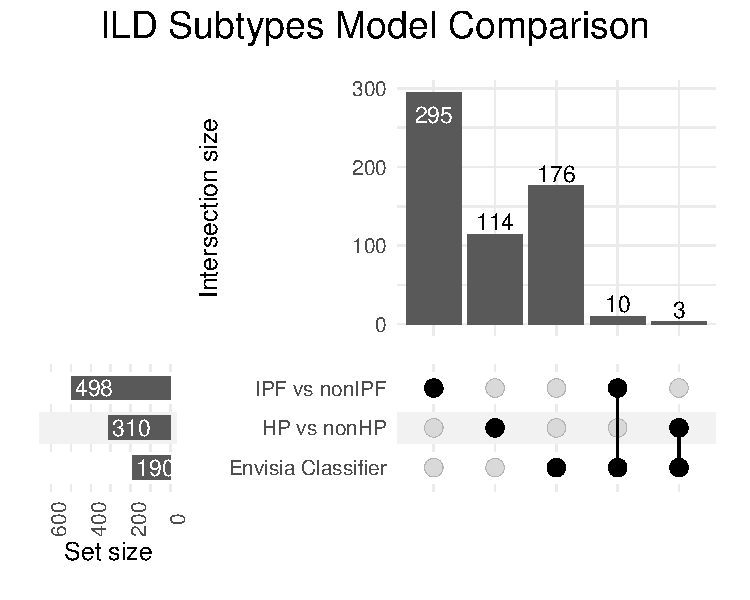
\includegraphics[width=0.6\linewidth,]{./Figures/SysReview/FigE10_Envisia} 

}

\caption[Envisia comparison]{\textbf{Upset plots of gene signatures featured in IPF vs non-IPF ILD and HP vs non-HP ILD expanded classifiers.} Genes from the Envisia classifier published in Choi et al.~(2017) are included as a comparison.}\label{fig:envisia}
\end{figure}

\clearpage

\hypertarget{appendix-b---supplementary-information-for-blood-biomarkers-pilot-study}{%
\subsection{Appendix B - Supplementary information for Blood Biomarkers Pilot Study}\label{appendix-b---supplementary-information-for-blood-biomarkers-pilot-study}}

\renewcommand{\thefigure}{A3.\arabic{figure}}
\setcounter{figure}{0}
\renewcommand{\thetable}{A3.\arabic{table}}
\setcounter{table}{0}
\renewcommand{\theequation}{A3.\arabic{equation}}
\setcounter{equation}{0}

\captionsetup{width=6.5in}

\hypertarget{differential-expression}{%
\subsection{Differential expression}\label{differential-expression}}



\begin{figure}

{\centering 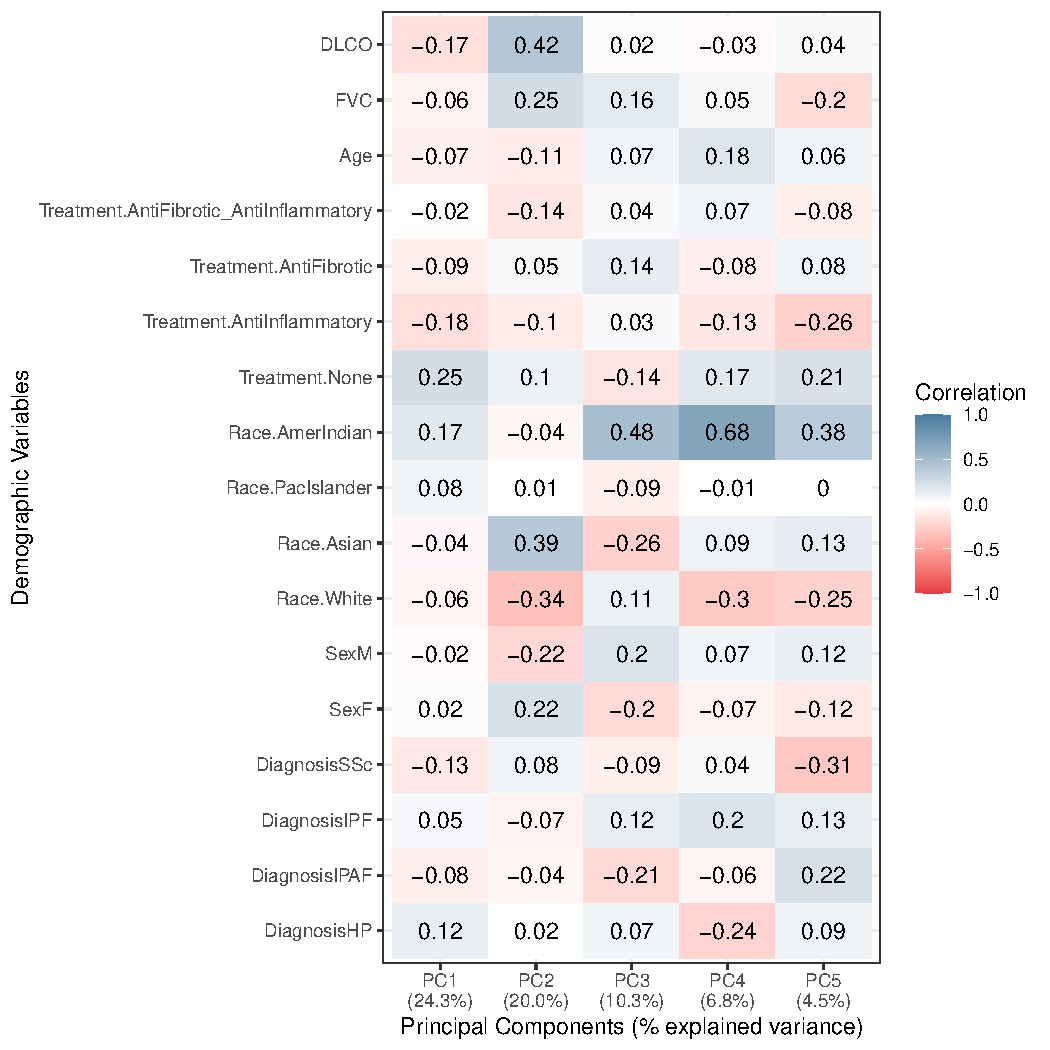
\includegraphics[width=0.8\linewidth,]{./Figures/BloodPilot/Figure E1 PCA metadata} 

}

\caption[Correlation of PCs with metadata (pilot study)]{\textbf{Correlation of principal component analysis (PCA) components (PCs) with demographic and clinical metadata.} Values shown are Pearson correlation coefficients.}\label{fig:pilotPCA}
\end{figure}



\begin{table}[!h]
\centering\centering
\caption{\label{tab:pilotpftdeg}\textbf{List of transcripts analyzed for differential expression with predicted forced vital capacity (FVC\%) and diffusing capacity of the lungs for carbon monoxide (DLCO\%).} Results shown are adjusted for using treatment status and race.}
\centering
\begin{tabu} to \linewidth {>{\raggedright\arraybackslash}p{0.8in}>{\raggedleft\arraybackslash}p{0.6in}>{\centering\arraybackslash}p{0.6in}>{\centering\arraybackslash}p{0.6in}>{\raggedright\arraybackslash}p{0.8in}>{\raggedleft\arraybackslash}p{0.6in}>{\centering\arraybackslash}p{0.6in}>{\centering\arraybackslash}p{0.6in}}
\toprule
\multicolumn{4}{c}{FVC\%} & \multicolumn{4}{c}{DLCO\%} \\
\cmidrule(l{3pt}r{3pt}){1-4} \cmidrule(l{3pt}r{3pt}){5-8}
Transcript & log\textsubscript{2}FC & \textit{p}-value & FDR & Transcript & log\textsubscript{2}FC & \textit{p}-value & FDR\\
\midrule
FOXJ1 & -0.013 & 0.001 & 0.106 & CD4 & 0.013 & 0.000 & 0.026\\
LTF & -0.022 & 0.004 & 0.106 & C9orf78 & -0.027 & 0.001 & 0.026\\
ITGA1 & -0.012 & 0.005 & 0.106 & ITGA1 & -0.016 & 0.001 & 0.026\\
PLA2G6 & -0.008 & 0.005 & 0.106 & DCAF6 & -0.013 & 0.001 & 0.026\\
TGFBI & 0.011 & 0.005 & 0.106 & CARM1 & -0.019 & 0.001 & 0.026\\
IRF2 & -0.007 & 0.005 & 0.106 & PLA2G6 & -0.011 & 0.001 & 0.026\\
IL1R1 & -0.011 & 0.007 & 0.106 & KLRF1 & -0.012 & 0.001 & 0.026\\
CECR1 & 0.010 & 0.007 & 0.106 & PLAGL2 & 0.008 & 0.001 & 0.026\\
SULT1A2 & -0.012 & 0.008 & 0.106 & SMAD2 & 0.007 & 0.002 & 0.039\\
CD4 & 0.009 & 0.008 & 0.106 & FOXJ1 & -0.014 & 0.003 & 0.039\\
RRAD & -0.014 & 0.008 & 0.106 & PSMF1 & -0.014 & 0.003 & 0.040\\
GBE1 & -0.007 & 0.008 & 0.106 & PPP3R1 & -0.012 & 0.004 & 0.048\\
LCN2 & -0.025 & 0.011 & 0.127 & SLC35E2B & 0.006 & 0.004 & 0.048\\
CYBB & 0.008 & 0.012 & 0.134 & FADD & -0.010 & 0.006 & 0.064\\
PDCD1 & -0.012 & 0.017 & 0.159 & ENTPD5 & -0.013 & 0.007 & 0.065\\
MAF & 0.008 & 0.018 & 0.159 & C1orf27 & 0.008 & 0.007 & 0.065\\
MPPED1 & -0.011 & 0.019 & 0.159 & IL1R1 & -0.012 & 0.009 & 0.081\\
FAM133B & -0.008 & 0.019 & 0.159 & TGFBI & 0.011 & 0.010 & 0.081\\
ENTPD5 & -0.010 & 0.022 & 0.173 & DAP & -0.008 & 0.010 & 0.081\\
KLRF1 & -0.008 & 0.023 & 0.173 & CHP1 & -0.010 & 0.011 & 0.081\\
GTF2H2 & -0.012 & 0.024 & 0.173 & RORC & 0.011 & 0.011 & 0.081\\
CMC1 & -0.007 & 0.026 & 0.177 & EWSR1 & 0.005 & 0.013 & 0.090\\
TEX261 & -0.006 & 0.027 & 0.180 & GTF2H2 & -0.015 & 0.014 & 0.096\\
BCL6 & -0.009 & 0.028 & 0.180 & IRF2 & -0.007 & 0.016 & 0.098\\
DCAF6 & -0.008 & 0.032 & 0.195 & CD59 & -0.008 & 0.016 & 0.098\\
\bottomrule
\end{tabu}
\end{table}

\newpage

\hypertarget{biomarker-panels}{%
\subsection{Biomarker panels}\label{biomarker-panels}}

\captionsetup{width=6.5in}



\begin{table}[!h]
\centering\centering
\caption{\label{tab:biomarkermodel}\textbf{Classification model performance on cross-validation for selected learning algorithms.} Data are reported as mean accuracy ± standard error.}
\centering
\begin{tabu} to \linewidth {>{\raggedright\arraybackslash}p{1.3in}>{\centering\arraybackslash}p{0.7in}>{\centering\arraybackslash}p{0.7in}>{\centering\arraybackslash}p{0.7in}}
\toprule
Comparison & sPLSDA & Elastic Net & Random Forest\\
\midrule
IPF vs non-IPF ILD & 0.62±0.01 & 0.70±0.02 & 0.65±0.02\\
IPF vs SSc-ILD & 0.74±0.01 & 0.80±0.02 & 0.65±0.02\\
IPF vs HP & 0.62±0.01 & 0.62±0.02 & 0.57±0.02\\
HP vs SSc-ILD & 0.60±0.01 & 0.68±0.02 & 0.64±0.02\\
\bottomrule
\end{tabu}
\end{table}

\newpage



\begin{table}[!h]
\centering\centering
\caption{\label{tab:biomarkerweight}\textbf{Coefficient weights of top 20 features (transcripts) of elastic net biomarker panels developed for each between-subtype comparison.}}
\centering
\begin{tabu} to \linewidth {>{\raggedright\arraybackslash}p{0.7in}>{\raggedleft\arraybackslash}p{0.6in}>{\raggedright\arraybackslash}p{0.7in}>{\raggedleft\arraybackslash}p{0.6in}>{\raggedright\arraybackslash}p{0.7in}>{\raggedleft\arraybackslash}p{0.6in}>{\raggedright\arraybackslash}p{0.7in}>{\raggedleft\arraybackslash}p{0.6in}}
\toprule
\multicolumn{2}{c}{IPF vs non-IPF} & \multicolumn{2}{c}{IPF vs SSc-ILD} & \multicolumn{2}{c}{IPF vs HP} & \multicolumn{2}{c}{HP vs SSc-ILD} \\
\cmidrule(l{3pt}r{3pt}){1-2} \cmidrule(l{3pt}r{3pt}){3-4} \cmidrule(l{3pt}r{3pt}){5-6} \cmidrule(l{3pt}r{3pt}){7-8}
Transcript & Weight & Transcript & Weight & Transcript & Weight & Transcript & Weight\\
\midrule
LTK & 0.484 & VCAN & -3.210 & CFD & 1.362 & GNLY & -1.400\\
VCAN & -0.412 & KLRF1 & -2.842 & HIP1 & -1.242 & RORC & 1.257\\
KLRF1 & -0.395 & DAP & 1.996 & LTK & -1.041 & CNTNAP3 & 0.838\\
CFD & -0.237 & LTK & 1.571 & CXCR6 & 0.963 & DAP & 0.764\\
LMBRD1 & 0.236 & FAM65B & -1.131 & RORC & 0.792 & HIP1 & -0.689\\
PLXNC1 & -0.235 & IL1R1 & -1.021 & VCAN & 0.703 & C9orf78 & 0.644\\
KRT23 & 0.225 & SCARNA5 & -0.977 & HLA-G & -0.556 & FCGR3A & 0.596\\
DAP & 0.163 & RORC & 0.863 & ITSN1 & 0.540 & KLRF1 & -0.592\\
C3AR1 & -0.140 & LMBRD1 & 0.811 & PTPN18 & 0.499 & CECR1 & 0.578\\
STAT6 & -0.137 & KRT23 & 0.810 & TNFRSF10C & 0.478 & SCARNA5 & -0.510\\
MAF & -0.112 & CTSS & 0.687 & MAP2K2 & 0.434 & SLC35E2B & 0.488\\
GATA3 & -0.107 & CECR1 & 0.656 & FCGR3A & 0.389 & VCAN & -0.459\\
SCARNA5 & -0.106 & FAM8A1 & 0.536 & PIK3CG & 0.373 & FADD & 0.456\\
TNFRSF10C & -0.104 & SEPT7 & -0.525 & GATA3 & 0.364 & MAF & 0.439\\
MAP2K2 & -0.104 & GNLY & -0.508 & CTDSP2 & 0.356 & PIK3CG & 0.430\\
CXCR6 & -0.088 & CISH & -0.439 & C3AR1 & 0.314 & ATP11A & 0.424\\
FAM8A1 & 0.069 & IL17A & -0.414 & MSN & 0.302 & RALGPS2 & -0.419\\
FAM65B & -0.060 & C3AR1 & -0.253 & STAT6 & 0.296 & LTK & -0.419\\
FUT7 & -0.055 & LILRA1 & 0.071 & SPARC & -0.284 & GATA3 & 0.418\\
GNLY & -0.040 & NAPA & -0.051 & HLA-A & 0.280 & GNAS & 0.405\\
\bottomrule
\end{tabu}
\end{table}

\clearpage

\hypertarget{appendix-c---supplementary-information-for-chapter-four}{%
\subsection{Appendix C - Supplementary information for Chapter Four}\label{appendix-c---supplementary-information-for-chapter-four}}

\renewcommand{\thefigure}{A4.\arabic{figure}}
\setcounter{figure}{0}
\renewcommand{\thetable}{A4.\arabic{table}}
\setcounter{table}{0}
\renewcommand{\theequation}{A4.\arabic{equation}}
\setcounter{equation}{0}

\end{document}
